\documentclass{BigNote}

\usetikzlibrary{arrows.meta}
\usetikzlibrary{calc}
\usetikzlibrary{braids}

\title{大笔记}
\author{我}

\addbibresource{BigNote.bib}
\usepackage{imakeidx}
\makeindex[columns=3, title=名词索引]

\begin{document}
    \maketitle

    \tableofcontents
    \newpage

    \chapter*{前言}
    
    此笔记意在记录学习中的一些命题证明以及想法.

    \chapter{基础知识}
    \section{逻辑}

断言 (statement) 是一类有明确真值 (T/F) 的语句, 我们定义如下运算:

\begin{definition}
    对于断言 \(A\) 定义其否定 (negation) 为 \(\neg A\), 满足如下真值表.
    \begin{center}
        \begin{tabular}{|c|c|}
            \hline
            \(A\) & \(\neg A\) \\
            \hline
            T & F \\
            \hline
            F & T \\
            \hline
        \end{tabular}
    \end{center}

    对于断言 \(A, B\) 定义其合取 (conjuction) 为 \(A \land B\), 其析取 (disjuction) 为 \(A \lor B\), 满足如下真值表.

    \begin{center}
        \begin{tabular}{|c|c|c|c|c|}
            \hline
            \(A\) & \(B\) & \(A \land B\) & \(A \lor B\) \\
            \hline
            T & T & T & T \\
            \hline
            T & F & F & T \\
            \hline
            F & T & F & T \\
            \hline
            F & F & F & F \\
            \hline
        \end{tabular}
    \end{center}
\end{definition}

\begin{definition}
    如果 \(E(x)\) 在 \(x\) 是某些对象时为断言, 则称 \(E(x)\) 为一个性质 (property).
\end{definition}

我们承认类 (class) 的概念如下, 若对象 \(x\) 属于类 \(A\), 则记为 \(x \in A\), 否则记为 \(x \notin A\).
我们用 \(\{x \in X; E(x)\}\) 表示 \(X\) 中所有满足性质 \(E\) 的对象组成的类.

\begin{definition}
    我们用 \(\exists\) 代表存在某个对象, 用 \(\forall\) 代表所有对象都满足某个性质.

    我们也用 \(\exists !\) 代表存在唯一一个对象.

    我们用 \(a := b\) 标记 \(a\) 由 \(b\) 定义, \(a = b\) 代表 \(a, b\) 仅仅是相同对象的两个表示 (集合论下会重新定义等于).
\end{definition}

我们有如下自明的公式.

\begin{theorem}
    \begin{align}
        \neg \neg A &:= \neg (\neg A) = A \\
        \neg (A \land B) &= \neg A \lor \neg B \\
        \neg (A \lor B) &= \neg A \land \neg B \\
        \neg (\forall x \in X : E(x)) &= \exists x \in X : \neg E(x) \\
        \neg (\exists x \in X : E(x)) &= \forall x \in X : \neg E(x) \\
        \neg (\forall x \in X : (\exists y \in Y : E(x, y))) &= \exists x \in X : (\forall y \in Y : \neg E(x, y)) \\
        \neg (\exists x \in X : (\forall y \in Y : E(x, y))) &= \forall x \in X : (\exists y \in Y : \neg E(x, y))
    \end{align}
\end{theorem}

\begin{definition}
    对于断言 \(A, B\), 我们记断言 \(A\) 能推出 \(B\) 为 \(A \implies B\), 代表
    \begin{equation}
        A \implies B := (\neg A) \lor B
    \end{equation}

    而断言 \(A, B\) 等价 (\(A \iff B\)) 意味着 \((A \implies B) \land (B \implies A)\).
\end{definition}

\begin{theorem}
    我们可以验证下述断言:
    \begin{align}
        (A \implies B) &\iff (\neg B \implies \neg A) \\
        (A \implies B) \land (B \implies C) &\implies (A \implies C)
    \end{align}
\end{theorem}

    \section{初等集合论}

朴素集合论认为

\begin{axiom}
    对于任意性质 \(P\) 均有 \(Y = \{x : P(x)\}\) 为集合.
\end{axiom}

然而随后提出的 Russell 悖论 (Russell's paradox) 给出了性质 \(X: X \notin X\) 对应的的集合不存在, 人们开始探索公理化集合论的道路. 

\subsection{von Neumann-Bernays-Gödel 公理}

von Neumann-Bernays-Gödel 公理系统的核心是类 (class) 与元素 (element), \(A\) 是 \(B\) 的元素用符号 \(A \in B\) 标记,
其否定自然使用 \(\notin\) 标记, 一个类可以作为另一个类的元素.

\begin{definition}
    两个类 \(A\) 与 \(B\) 相等, 记作 \(A = B\), 当且仅当 \(A\) 与 \(B\) 有相同的元素, 其否定记为 \(A \neq B\).

    \[
        (X = Y) := \forall Z (Z \in X \iff Z \in Y)
    \]
\end{definition}

\begin{corollary}
    显见以下公式:

    \begin{enumerate}
        \item \(\forall X (X = X)\)
        \item \(\forall X \forall Y (X = Y \implies Y = X)\)
        \item \(\forall X \forall Y \forall Z ((X = Y \land Y = Z) \implies X = Z)\)
    \end{enumerate}
\end{corollary}

\begin{definition}
    一个类 \(A\) 是另一个类 \(B\) 的子类, 记作 \(A \subseteq B\), 当且仅当 \(A\) 的所有元素都是 \(B\) 的元素, 其否定记为 \(A \nsubseteq B\).

    \[
        (X \subseteq Y) := \forall Z (Z \in X \implies Z \in Y)
    \]

    我们用 \(A \subset B\) 表示 \(A \subseteq B \land A \neq B\), 称非空 \(A \subset B\) 为真子类.
\end{definition}

\begin{corollary}
    \[
        (X \subseteq Y) \land (Y \subseteq X) \iff (X = Y)
    \]
\end{corollary}

\begin{axiom}[Axiom of Equality]
    \setlabel {Axiom of Equality}
    \label {axiom:NBG Axiom of Equality}
    \[
        \forall X \forall Y (X = Y \implies \forall Z (X \in Z \iff Y \in Z))
    \]
\end{axiom}

\begin{definition}[集合]
    一个类 \(X\) 称集合 (set), 当且仅当 \(\exists Y (X \in Y)\), 本节中我们用小写字母 \(x, y, z, \dots\) 表示集合, 用大写字母 \(X, Y, Z, \dots\) 表示类.
\end{definition}

\begin{definition}[真类]
    一个类 \(X\) 称真类 (proper class), 当且仅当 \(X\) 不是集合, 常用粗体字母 \(\mathbf{X}, \mathbf{Y}, \mathbf{Z}, \dots\) 表示真类.
\end{definition}

\begin{axiom}[Axiom of Pair]
    \setlabel {Axiom of Pair}
    \label {axiom:NBG Axiom of Pair}
    \[
        \forall x \forall y \exists z \forall u (u \in z \iff (u = x \lor u = y))
    \]
\end{axiom}

上述公理展开可得 \(\forall x \forall y ((\exists X \exists Y (x \in X \land y \in Y)) \implies \exists z \exists Z (z \in Z \land \forall u (u \in Z \iff (u = x \lor u = y))))\),
记集合 \(z = \{x,y\}\), 特别的, 当 \(x = y\) 时, 我们记 \(z = \{x\}\).

为了方便叙述, 我们常常忽略公式最前的 \(\forall\)

\begin{corollary}
    显见以下公式:

    \begin{enumerate}
        \item \(((x = u \land y = v) \implies \{x,y\} = \{u,v\})\)
        \item \(\{x,y\} = \{y,x\}\).
        \item \(x = y \iff \{x\} = \{y\}\).
        \item \(x = y \iff \forall Z (x \in Z \iff y \in Z)\).
    \end{enumerate}
\end{corollary}

\begin{definition}[有序对]
    \label {definition:Kuratowski ordered pair}
    有序对 (ordered pair) \((x,y)\) 定义为 \(\{\{x\},\{x,y\}\}\).
\end{definition}

\begin{lemma}
    有序对的有序体现在其性质 \((x,y) = (u,v) \iff (x = u \land y = v)\).

    \begin{proof}
        \((\impliedby)\) 显然.

        \((\implies)\) 若 \(x \neq u\), 则 \(\{x\} \neq \{u\}\), 依赖 \ref{axiom:NBG Axiom of Pair}
        \(\{x\} \in (x,y) = (u,v)\), 从而 \(u \in \{u, v\} = \{x\}\), 矛盾.

        若 \(x = u \land y \neq v\), 只需证明 \(a = b \iff \{c,a\} = \{c,b\}\), 
        由 \ref{axiom:NBG Axiom of Pair} 知 \(a \in \{c,a\} = \{c,b\}\) 从而 \(a = c\), 同理, 
        \(b = c\), 矛盾.
    \end{proof}
\end{lemma}

\begin{definition}[有序三元对]
    \label {definition:ordered triple}
    有序三元对 (ordered triple) \((x,y,z)\) 定义为有序对 \(((x,y),z)\).
\end{definition}

\begin{definition}[二元关系]
    \label {definition:binary relation}
    类 \(R\) 称二元关系 (binary relation), 当且仅当 \(R\) 是有序对的集合, 记作 \(\mathbf{isbinrel} (R)\).

    \[
        \mathbf{isbinrel} (R) \iff \forall z (z \in R \implies \exists x \exists y (z = (x,y)))
    \]
\end{definition}

在不久的将来, 我们将用二元关系定义映射.

\begin{axiom}[Axiom of Membership]
    \setlabel {Axiom of Membership}
    \label {axiom:NBG Axiom of Membership}
    \[
        \exists \mathfrak{E} \forall z (z \in \mathfrak{E} \iff \exists x \exists y (z = (x,y) \land x \in y))
    \]
\end{axiom}

\begin{axiom}[Axiom of Domain]
    \setlabel {Axiom of Domain}
    \label {axiom:NBG Axiom of Domain}
    \[
        \forall X \exists D \forall x (x \in D \iff \exists y ((x,y) \in X))
    \]
\end{axiom}

\begin{definition}
    \label {definition:domain}
    上述定义中类 \(D\) 称为 \(X\) 的定义域 (domain), 记作 \(\mathbf{dom} (X)\).
\end{definition}

\begin{definition}
    \label {definition:universe}
    定义 \(\mathfrak{U} := \mathbf{dom} (\mathfrak{E})\), 称为宇宙 (universe), 注意到 \(\forall x (x \in \{x\})\),
    从而 \(\forall x (x \in \mathfrak{U})\).
\end{definition}

\begin{corollary}
    \[
        \mathbf{dom} (\mathfrak{U}) = \mathfrak{U}
    \]
\end{corollary}

\begin{axiom}[Axiom of Difference]
    \setlabel {Axiom of Difference}
    \label {axiom:NBG Axiom of Difference}
    \[
        \forall X \forall Y \exists D \forall x (x \in D \iff (x \in X \land x \notin Y))
    \]
\end{axiom}

\begin{definition}
    \label {definition:difference of two classes}
    上述定义中类 \(D\) 称为 \(X\) 与 \(Y\) 的差集 (difference), 记作 \(X \setminus Y\).
\end{definition}

\begin{definition}
    \label {definition:intersection of two classes}
    定义 \(X \cap Y := X \setminus (X \setminus Y)\), 称为 \(X\) 与 \(Y\) 的交集 (intersection).
\end{definition}

\begin{definition}
    \label {definition:union of two classes}
    定义 \(X \cup Y := \mathfrak{U} \setminus ((\mathfrak{U} \setminus X) \cap (\mathfrak{U} \setminus Y))\), 称为 \(X\) 与 \(Y\) 的并集 (union).
\end{definition}

\begin{definition}
    \label {definition:symmetric difference of two classes}
    定义 \(X \triangle Y := (X \setminus Y) \cup (Y \setminus X)\), 称为 \(X\) 与 \(Y\) 的对称差 (symmetric difference).
\end{definition}

\begin{definition}
    \label {definition:empty class}
    定义 \(\varnothing := \mathfrak{U} \setminus \mathfrak{U}\), 称为空类 (empty class), 根据 \ref{axiom:ZF Axiom of Infinity} 空类是集合 (空集, empty set).
\end{definition}

\begin{corollary}
    \[
        \forall E (\varnothing = E \setminus E)
    \]

    \begin{proof}
        运用 \ref{axiom:NBG Axiom of Equality} 即可.
    \end{proof}
\end{corollary}

\begin{axiom}[Axiom of Product]
    \setlabel {Axiom of Product}
    \label {axiom:NBG Axiom of Product}
    \[
        \forall X \forall Y \exists P \forall z (z \in P \iff \exists x \exists y (z = (x,y) \land x \in X \land y \in Y))
    \]
\end{axiom}

\begin{definition}
    \label {definition:product of two classes}
    上述定义中类 \(P\) 称为 \(X\) 与 \(Y\) 的积 (product), 记作 \(X \times Y\).
\end{definition}

\begin{definition}
    定义宇宙的积 \(\mathfrak{U} \times \mathfrak{U} := \ddot {\mathfrak{U}}\),
    此时 \(\mathbf{isbinrel} (R) \iff R \subseteq \ddot {\mathfrak{U}}\).
\end{definition}

\begin{axiom}[Axiom of Inversion]
    \setlabel {Axiom of Inversion}
    \label {axiom:NBG Axiom of Inversion}
    \[
        \forall X \exists I \forall z (z \in I \iff \exists x \exists y (z = (x,y) \land (y,x) \in X))
    \]
\end{axiom}

\begin{axiom}[Axiom of Cycle]
    \setlabel {Axiom of Cycle}
    \label {axiom:NBG Axiom of Cycle}
    \[
        \forall X \exists C \forall t (t \in C \iff \exists x \exists y \exists z (t = (z,x,y) \land (x,y,z) \in X))
    \]
\end{axiom}

\begin{definition}
    由上述公理定义的 \(I\) 记作 \(X^{-1}\), 称为 \(X\) 的逆 (inverse), \(C\) 记作 \(X^{\circlearrowright}\), \(X^{\circlearrowleft} := {(X^{\circlearrowright})}^{\circlearrowright}\).
\end{definition}

\begin{definition}
    \label {definition:range}
    定义 \(\mathbf{ran} (X) := \mathbf{dom} (X^{-1})\), 称为 \(X\) 的值域 (range).
\end{definition}

\begin{definition}
    \label{definition:union of classes}
    定义类 \(X\) 的并 (union) \(\bigcup X := \{z : \exists y \in X (z \in y)\}\).
    \label{definition:intersection of classes}
    定义类 \(X\) 的交 (intersection) \(\bigcap X := \{z : \forall y \in X (z \in y)\}\).
    \label{definition:power class}
    定义类 \(X\) 的幂 (power) \(\mathcal{P} (X) := \{Y : Y \subseteq X\}\).

    这里用到对类的表示方法, \(\{x : \phi (x)\}\) 表示满足条件 \(\phi (x)\) 的所有元素的类.

    \begin{proof}
        存在性依次由以下三者给出:

        \[
            \bigcup X = \mathbf{dom} (\mathfrak{E} \cap (\mathfrak{U} \times X))
        \]

        \[
            \bigcap X = \mathfrak{U} \setminus \mathbf{dom} ((\ddot {\mathfrak{U}} \setminus \mathfrak{E}) \cap (\mathfrak{U} \times X))
        \]

        \[
            \mathcal{P} (X) = \mathfrak{U} \setminus \mathbf{dom} (\mathfrak{E}^{-1} \cap (\mathfrak{U} \times (\mathfrak{U} \setminus X)))
        \]
    \end{proof}
\end{definition}

\begin{corollary}
    \[
        \mathcal{P} (\mathfrak{U}) = \mathfrak{U}
    \]
\end{corollary}

\begin{definition}
    \label {definition:image of a class}
    给出类 \(X\) 与二元关系 \(R\), 定义 \(X\) 在 \(R\) 下的像 (image) \(R[X] := \{y : \exists x \in X ((x,y) \in R)\} = \mathbf{ran} [R \cap (X \times \mathfrak{U})]\).

    \label {definition:preimage of a class}
    同理定义其逆像 (preimage) \(R^{-1}[X]\).
\end{definition}

\begin{definition}
    \label {definition:composition of two classes}
    给出二元关系 \(F, G\), 定义 \(F\) 与 \(G\) 的复合 (composition) \(F \circ G := \{(x,z) : \exists y ((x,y) \in G \land (y,z) \in F)\}\).

    \begin{proof}
        \[
            F \circ G = \mathbf{dom} ({(G^{-1} \times \mathfrak{U})}^{\circlearrowleft} \cup {(F^{-1} \times \mathfrak{U})}^{\circlearrowright})
        \]
    \end{proof}
\end{definition}

\begin{definition}
    \label {definition:function (set)}
    映射 (function) \(f\) 定义为满足 \((x,y) \in f \land (x,y^\prime) \in f \implies y = y^\prime\) 的二元关系, 记作 \(\mathbf{isfunc} (f)\).

    在存在 \(y\) 的情况下我们记 \(f(x)\) 为唯一的 \(y\) 使得 \((x,y) \in f\), 称为 \(f\) 在 \(x\) 处的值 (value), 映射有时也称函数.
\end{definition}

\begin{definition}
    \label {definition:injective (set)}
    单射 (injective) 指代 \(f, f^{-1}\) 都是映射的二元关系 \(f\).
\end{definition}

\begin{corollary}
    给出映射 \(F, G\), \(F \circ G\) 也是映射.
\end{corollary}

接下来从类转向集合, 定义集合的操作与要求.

\begin{axiom}[Axiom of Replacement]
    \setlabel {Axiom of Replacement}
    \label {axiom:NBG Axiom of Replacement}
    \[
        \forall x \forall F (\mathbf{isfunc} (F) \implies \exists y (y = F[x]))
    \]
\end{axiom}

\begin{axiom}[Axiom of Union]
    \setlabel {Axiom of Union}
    \label {axiom:NBG Axiom of Union}
    \[
        \forall x \exists y (y = \bigcup x)
    \]
\end{axiom}

\begin{axiom}[Axiom of Power Set]
    \setlabel {Axiom of Power Set}
    \label {axiom:NBG Axiom of Power Set}
    \[
        \forall x \exists y (y = \mathcal{P} (x))
    \]
\end{axiom}

\begin{axiom}[Axiom of Infinity]
    \setlabel {Axiom of Infinity}
    \label {axiom:NBG Axiom of Infinity} (存在归纳集)
    \[
        \exists x (\varnothing \in x \land \forall y (y \in x \implies y \cup \{y\} \in x))
    \]
\end{axiom}

\begin{axiom}[Axiom of Foundation]
    \setlabel {Axiom of Foundation}
    \label {axiom:NBG Axiom of Foundation}
    \[
        \forall x (x \neq \varnothing \implies \exists y (y \in x \land y \cap x = \varnothing))
    \]
\end{axiom}

\begin{axiom}[Axiom of Global Choice]
    \setlabel {Axiom of Global Choice}
    \label {axiom:NBG Axiom of Global Choice}
    \[
        \exists f (\mathbf{isfunc} (f) \land \forall x (x \neq \varnothing \implies \exists y (y \in x \land (x,y) \in f)))
    \]
\end{axiom}

上述 \ref{axiom:NBG Axiom of Global Choice} 有个弱化版本如下:

\begin{axiom}[Axiom of Choice]
    \setlabel {Axiom of Choice}
    \label {axiom:NBG Axiom of Choice}
    \[
        \forall x \exists f (\mathbf{isfunc} (f) \land \forall y ((y \in x \land y \neq \varnothing) \implies \exists z ((y,z) \in f \land z \in y)))
    \]
\end{axiom}

称满足上述定理要求的映射 \(f\) 为 \(x\) 上的选择函数 (choice function).

NBG 公理 \cite{TarasBanakh:ClassicalSetTheory} 由以下 14 条公理组成:

\begin{enumerate}
    \item \ref{axiom:NBG Axiom of Equality}
    \[
        \forall X \forall Y (X = Y \implies \forall Z (X \in Z \iff Y \in Z))
    \]
    \item \ref{axiom:NBG Axiom of Pair}
    \[
        \forall x \forall y \exists z \forall u (u \in z \iff (u = x \lor u = y))
    \]
    \item \ref{axiom:NBG Axiom of Membership}
    \[
        \exists \mathfrak{E} \forall z (z \in \mathfrak{E} \iff \exists x \exists y (z = (x,y) \land x \in y))
    \]
    \item \ref{axiom:NBG Axiom of Domain}
    \[
        \forall X \exists D \forall x (x \in D \iff \exists y ((x,y) \in X))
    \]
    \item \ref{axiom:NBG Axiom of Difference}
    \[
        \forall X \forall Y \exists D \forall x (x \in D \iff (x \in X \land x \notin Y))
    \]
    \item \ref{axiom:NBG Axiom of Product}
    \[
        \forall X \forall Y \exists P \forall z (z \in P \iff \exists x \exists y (z = (x,y) \land x \in X \land y \in Y))
    \]
    \item \ref{axiom:NBG Axiom of Inversion}
    \[
        \forall X \exists I \forall z (z \in I \iff \exists x \exists y (z = (x,y) \land (y,x) \in X))
    \]
    \item \ref{axiom:NBG Axiom of Cycle}
    \[
        \forall X \exists C \forall t (t \in C \iff \exists x \exists y \exists z (t = (z,x,y) \land (x,y,z) \in X))
    \]
    \item \ref{axiom:NBG Axiom of Replacement}
    \[
        \forall x \forall F (\mathbf{isfunc} (F) \implies \exists y (y = F[x]))
    \]
    \item \ref{axiom:NBG Axiom of Union}
    \[
        \forall x \exists y (y = \bigcup x)
    \]
    \item \ref{axiom:NBG Axiom of Power Set}
    \[
        \forall x \exists y (y = \mathcal{P} (x))
    \]
    \item \ref{axiom:NBG Axiom of Infinity}
    \[
        \exists x (\varnothing \in x \land \forall y (y \in x \implies y \cup \{y\} \in x))
    \]
    \item \ref{axiom:NBG Axiom of Foundation}
    \[
        \forall x (x \neq \varnothing \implies \exists y (y \in x \land y \cap x = \varnothing))
    \]
    \item \ref{axiom:NBG Axiom of Global Choice}
    \[
        \exists f (\mathbf{isfunc} (f) \land \forall x (x \neq \varnothing \implies \exists y (y \in x \land (x,y) \in f)))
    \]
\end{enumerate}

我们借由 NBG 公理给出一些推论:

\begin{corollary}
    \label {corollary:no infinite descending chain}
    不存在无限降链 (infinite descending chain) \(x_0 \supset x_1 \supset x_2 \supset \dots\), 且不存在 \(x \in x\).

    \begin{proof}
        由 \ref{axiom:NBG Axiom of Foundation}.
    \end{proof}
\end{corollary}

\begin{corollary}
    \label {corollary:NBG every set can be separated by a class}
    集合的子集是集合, 从而集合 \(x\) 与类 \(C\) 的交 \(x \cap C\) 也是集合.

    这里的做法在于使用 \ref{axiom:NBG Axiom of Power Set} 并且意识到 \(y \subseteq x \implies y \in \mathcal{P} (x)\).
\end{corollary}

\begin{corollary}
    \label {corollary:NBG every property can be written as a class}
    我们说明如何把任何一个性质都写作类, 从而我们可以对一个集合进行分离操作, 也即我们给出类 \(\{x : \phi(x,p_1,p_2 \cdots p_n)\}\).

    \begin{proof}
        我们总是将 \(\forall x\) 认作 \(\neg \exists x\), 我们给出一种归纳方法,
        假定公式中有 \(n\) 个变元, 考察 \(\mathfrak{Un} := \mathfrak{U} \times \mathfrak{U} \times \dots \times \mathfrak{U}\) 上的类,
        并且已经将一部分的命题转为类 \(P\), 命题的否定无非是 \(\mathfrak{Un} \setminus P\), 命题的析取无非是 \(P_1 \cap P_2\),
        命题的合取无非是 \(P_1 \cup P_2\), 两个类属于引导出将 \(\mathfrak{E} \times \mathfrak{U} \times \mathfrak{U} \dots \mathfrak{U}\) 上多次施以
        \ref{axiom:NBG Axiom of Cycle} 与 \ref{axiom:NBG Axiom of Inversion} 的结果, 利用 \ref{axiom:NBG Axiom of Domain} 可以丢弃用完的变量.
        从而我们可以将任何命题转为类, 于是可以有集合 \(\{z \in x : P(z)\}\).
    \end{proof}
\end{corollary}

另外的, 将 NBG 公理中的 \ref{axiom:NBG Axiom of Membership}, \ref{axiom:NBG Axiom of Domain},
\ref{axiom:NBG Axiom of Difference}, \ref{axiom:NBG Axiom of Product}, \ref{axiom:NBG Axiom of Inversion},
\ref{axiom:NBG Axiom of Cycle} 替换为以下公理, 我们得到了 BGC 公理, 其与 NBG 等价:

\begin{axiom}[Axiom of Comprehension]
    \setlabel {Axiom of Comprehension}
    \label {axiom:BG Axiom of Comprehension}
    \[
        \forall X_1 \forall X_2 \dots \forall X_n \exists Y (Y = \{x : \phi (x,X_1,X_2, \dots,X_n)\})
    \]
\end{axiom}

更细致的讨论见本章末尾.

\subsection{基本构造}

\begin{corollary}
    集合的子类是集合.

    \begin{proof}
        对 \(X \subseteq y\) 有 \(X \in \mathcal{P} (y)\).
    \end{proof}
\end{corollary}

\begin{definition}
    \label {definition:union of two sets}
    集合 \(x\) 与 \(y\) 的并定义为 \(x \cup y := \bigcup \{x,y\}\).
\end{definition}

\begin{definition}
    \label {definition:intersection of two sets}
    集合 \(x\) 与 \(y\) 的交 \(x \cap y\) 也是集合.

    \begin{proof}
        根据 \ref{corollary:NBG every set can be separated by a class}.
    \end{proof}
\end{definition}

\begin{definition}
    \label {definition:difference of two sets}
    集合 \(x\) 与 \(y\) 的差集 \(x \setminus y\) 是一个集合.

    \begin{proof}
        对 \(x, \mathfrak{U} \setminus y\) 应用 \ref{corollary:NBG every set can be separated by a class}.
    \end{proof}
\end{definition}

\begin{definition}
    \label {definition:product of two sets}
    集合 \(x\) 与 \(y\) 的积 \(x \times y\) 是一个集合.

    \begin{proof}
        \(x \times y \subseteq \mathcal{P} \mathcal{P} (x \cup y)\), 从而是一个集合.
    \end{proof}
\end{definition}

\begin{definition}
    \label {definition:function from a set to a set}
    集合 \(x\) 到 \(y\) 的全体映射 \(y^x\) 构成一个集合.

    \begin{proof}
        \(f \subseteq x \times y\), 从而是一个集合.
    \end{proof}
\end{definition}

\begin{definition}
    \label {definition:surjective (set)}
    对于 \(x,y\) 与 \(f : x \to y\), \(f\) 是满射 (surjective), 当且仅当 \(f[x] = y\).
\end{definition}

\begin{definition}
    存在类 \(\mathfrak{Rel} := \{r : \mathbf{isbinrel} (r)\}\) 为全体二元关系集构成的类.

    \begin{proof}
        \[
            \mathfrak{Rel} = \mathfrak{U} \setminus \mathbf{dom} ((\mathfrak{E}^{-1} \setminus \mathfrak{U} \times (\mathfrak{U} \times \mathfrak{U})))
        \]
    \end{proof}
\end{definition}

以下证明写起来过于冗长, 读者可自行运用 \ref{theorem:Gödel class existence} 进行验证.

\begin{definition}
    存在类 \(\mathfrak{Func} := \{f : \mathbf{isfunc} (f)\}\) 为全体映射集构成的类.
\end{definition}

\begin{definition}
    对于类 \(A,X\) 亦定义 \(X^A\) 为 \(A\) 到 \(X\) 的全体映射构成的类.
\end{definition}

\begin{definition}
    对一个 \(X \subseteq A \times \mathfrak{U}\), 可以视作一组以 \(A\) 为指标的集合 \({(X_\alpha)}_{\alpha \in A}\).
    定义 \(\bigcup_{\alpha \in A} X_\alpha = \mathbf{ran} (X)\), \(\bigcap_{\alpha \in A} X_\alpha = \mathbf{dom} (X)\).

    也可以视作多值函数 (multifunction) \(X : A \multimap \mathfrak{U}\) 给 \(\alpha \in A\) 值 \(X[\{\alpha\}]\),
    并且对 \(B \subseteq A\) 给出 \(X[B] = \mathbf{ran} (X \cap (B \times \mathfrak{U}))\).
\end{definition}

\begin{definition}[笛卡尔积]
    \label {definition:cartesian product}
    对于类 \(A,X \subseteq A \times \mathfrak{U}\), 定义 \(\prod_{\alpha \in A} X_\alpha := \{f \in \mathfrak{Func} : \forall (\alpha \in A)(f(\alpha) \in X_\alpha) \land (\mathbf{dom} (f) = A)\}\), 称为 \(X = (X_\alpha)_{\alpha \in A}\) 的笛卡尔积 (cartesian product).
\end{definition}

真类 \(A\) 诱导出的笛卡尔积是空类.

\begin{definition}[无交并]
    \label {definition:disjoint union}
    对于类 \(A,X \subseteq A \times \mathfrak{U}\), 定义 \(\coprod_{\alpha \in A} X_\alpha := \{(x,y) \in \mathfrak{U} \times A : x \in X_y\}\), 称为 \(X = (X_\alpha)_{\alpha \in A}\) 的无交并 (disjoint union).
\end{definition}

\subsection{Zermelo-Fraenkel 公理}

与 NBG 公理思路不同的是 ZF 公理, ZF 公理体系没有 NBG 公理中类的概念, 或者说 ZF 公理体系中的类 \(C\) 代
指一个有单个自由变量的命题 \(x \in C := \phi(x, p_1, p_2 \dots)\), 其中 \(p_1, p_2 \dots\) 是给定参数.

相应的, 类的运算被视作逻辑命题的计算.

\begin{definition}
    \label {definition:ZF universe}
    定义 \(\mathfrak{U} := \{x : x = x\}\), 称为宇宙 (universe).
    \label {definition:ZF subclass}
    定义 \(X \subseteq Y := \forall x (x \in X \implies x \in Y)\), 称为 \(X\) 是 \(Y\) 的子类 (subclass).
    \label {definition:ZF class intersection}
    定义 \(\bigcap X := \{x : \forall y \in X (x \in y)\}\), 称为 \(X\) 的交集 (intersection).
    \label {definition:ZF class union}
    定义 \(\bigcup X := \{x : \exists y \in X (x \in y)\}\), 称为 \(X\) 的并集 (union).
    \label {definition:ZF power class}
    定义 \(\mathcal{P} (X) := \{Y : Y \subseteq X\}\), 称为 \(X\) 的幂 (power).
    \label {definition:ZF class difference}
    定义 \(X \setminus Y := \{x : x \in X \land x \notin Y\}\), 称为 \(X\) 与 \(Y\) 的差集 (difference).
\end{definition}

此意义上, 集合自然是类 \(\{x:x \in S\}\), ZF 公理包含 (本节大写字母亦表示集合):

\begin{axiom}[Axiom of Extensionality]
    \setlabel {ZFC Axiom of Extensionality}
    \label {axiom:ZF Axiom of Extensionality}
    \[
        \forall X \forall Y (\forall z (z \in X \iff z \in Y) \implies X = Y)
    \]
\end{axiom}

\begin{axiom}[Axiom of Pair]
    \setlabel {ZFC Axiom of Pair}
    \label {axiom:ZF Axiom of Pair}
    \[
        \forall X \forall Y \exists Z \forall U (U \in Z \iff (U = X \lor U = Y))
    \]
\end{axiom}

\begin{axiom}[Axiom of Union]
    \setlabel {ZFC Axiom of Union}
    \label {axiom:ZF Axiom of Union}
    \[
        \forall X \exists Y \forall z (z \in Y \iff \exists u \in X (z \in u))
    \]
\end{axiom}

\begin{axiom}[Axiom of Power Set]
    \setlabel {ZFC Axiom of Power Set}
    \label {axiom:ZF Axiom of Power Set}
    \[
        \forall X \exists Y \forall z (z \in Y \iff z \subseteq X)
    \]
\end{axiom}

\begin{axiom}[Axiom Schema of Separations]
    \setlabel {ZFC Axiom Schema of Separations}
    \label {axiom:ZF Axiom Schema of Separations}
    \[
        \forall X \exists Y \forall z (z \in Y \iff (z \in X \land \phi (z)))
    \]
\end{axiom}

寻此几条公理, 我们仍然可以仿照 NBG 公理进行一些定义, 不过我们要给一个集合作为基础:

\begin{definition}
    \label {definition:ZF empty set}
    空集 (empty set) 定义为 \(\varnothing := \{x \in X : x \neq x\}\), 此中要求至少存在一个集合.

    \label {definition:ZF ordered pair}
    有序对 (ordered pair) \((x,y)\) 定义为 \(\{\{x\},\{x,y\}\}\).

    \label {definition:ZF ordered triple}
    有序三元对 (ordered triple) \((x,y,z)\) 定义为 \(((x,y),z)\).

    \label {definition:ZF set product}
    集合 \(X\) 与 \(Y\) 的积 (product) 定义为 \(X \times Y := \{(x,y) : x \in X \land y \in Y\}\),
    可以由 \(\mathcal{P} (\mathcal{P} (X \cup Y))\) 上用分离公理给出.

    \label {definition:ZF binary relation}
    \(X\) 上的二元关系 (binary relation) 定义为 \(R \subseteq X \times X\).

    \label {definition:ZF function}
    映射 (function) 定义为一个有序对构成的类 \(f\), 且满足
    \(\forall x \forall y \forall z (((x,y) \in f \land (x,z) \in f) \implies (y = z))\).

    映射自然延拓至类, 定义为满足以上唯一性条件且每个元素都是有序对的类.

    \label {definition:ZF image}
    \(X\) 在 \(f\) 下的像 (image) 定义为 \(f[X] := \{y : \exists x \in X ((x,y) \in f)\}\).
\end{definition}

\begin{axiom}[Axiom of Infinity]
    \setlabel {ZFC Axiom of Infinity}
    \label {axiom:ZF Axiom of Infinity}
    \[
        \exists x (\varnothing \in x \land \forall y (y \in x \implies y \cup \{y\} \in x))
    \]
\end{axiom}

\begin{axiom}[Axiom Schema of Replacement]
    \setlabel {ZFC Axiom Schema of Replacement}
    \label {axiom:ZF Axiom Schema of Replacement}
    \[
        \forall f \forall x (\mathbf{isfunc} (f) \implies \exists y (y = f[x]))
    \]
\end{axiom}

\begin{axiom}[Axiom of Regularity]
    \setlabel {ZFC Axiom of Regularity}
    \label {axiom:ZF Axiom of Regularity}
    \[
        \forall x (x \neq \varnothing \implies \exists y (y \in x \land y \cap x = \varnothing))
    \]
\end{axiom}

ZF 公理 \cite{ThomasJech:SetTheory} 代指以下 8 条公理:

\begin{enumerate}
    \item \ref{axiom:ZF Axiom of Extensionality}
    \[
        \forall X \forall Y (\forall z (z \in X \iff z \in Y) \implies X = Y)
    \]
    \item \ref{axiom:ZF Axiom of Pair}
    \[
        \forall X \forall Y \exists Z \forall U (U \in Z \iff (U = X \lor U = Y))
    \]
    \item \ref{axiom:ZF Axiom of Union}
    \[
        \forall X \exists Y \forall z (z \in Y \iff \exists u \in X (z \in u))
    \]
    \item \ref{axiom:ZF Axiom of Power Set}
    \[
        \forall X \exists Y \forall z (z \in Y \iff z \subseteq X)
    \]
    \item \ref{axiom:ZF Axiom Schema of Separations}
    \[
        \forall X \exists Y \forall z (z \in Y \iff (z \in X \land \phi (z)))
    \]
    \item \ref{axiom:ZF Axiom of Infinity}
    \[
        \exists x (\varnothing \in x \land \forall y (y \in x \implies y \cup \{y\} \in x))
    \]
    \item \ref{axiom:ZF Axiom Schema of Replacement}
    \[
        \forall f \forall x (\mathbf{isfunc} (f) \implies \exists y (y = f[x]))
    \]
    \item \ref{axiom:ZF Axiom of Regularity}
    \[
        \forall x (x \neq \varnothing \implies \exists y (y \in x \land y \cap x = \varnothing))
    \]
\end{enumerate}

囊括以下选择公理的体系称为 ZFC 公理:

\begin{axiom}[Axiom of Choice]
    \setlabel {ZFC Axiom of Choice}
    \label {axiom:ZF Axiom of Choice}
    \[
        \forall x \exists f (\mathbf{isfunc} (f) \land \forall y (y \in x \implies \exists z ((y,z) \in f)))
    \]
\end{axiom}

可以发现, NBG 公理中对类操作的 \ref{axiom:NBG Axiom of Equality}, \ref{axiom:NBG Axiom of Membership},
\ref{axiom:NBG Axiom of Domain}, \ref{axiom:NBG Axiom of Difference}, \ref{axiom:NBG Axiom of Product},
\ref{axiom:NBG Axiom of Inversion}, \ref{axiom:NBG Axiom of Cycle}, 在 ZFC 下体现为类背后的逻辑命题的计算,
而 \ref{axiom:NBG Axiom of Pair}, \ref{axiom:NBG Axiom of Union}, \ref{axiom:NBG Axiom of Power Set},
\ref{axiom:NBG Axiom of Infinity}, \ref{axiom:NBG Axiom of Foundation}, \ref{axiom:NBG Axiom of Choice}
在 ZFC 下体现为集合的操作与要求.

可以证明在只考虑集合的情况下, ZFC 公理与 NBG 公理等价, 我们将选取 NBG 公理, 因为一定程度上 NBG 公理表述更加方便, 严格给出了 "类" 的概念, 而非 ZFC 公理中的一个 "语法糖".

\subsection{序数}

序数几乎是集合论上唯一的结构, 有必要对其进行研究.

\subsubsection{偏序}

\begin{definition}
    一个等价关系 \(\sim\) 是满足自反性 (reflexivity), 对称性 (symmetry), 传递性 (transitivity) 的二元关系.
    \begin{enumerate}
        \item 自反性 (reflexivity): \(x \sim x\).
        \item 对称性 (symmetry): \(x \sim y \implies y \sim x\).
        \item 传递性 (transitivity): \(x \sim y \land y \sim z \implies x \sim z\).
    \end{enumerate}


    等价关系给出了集合的一个划分, 也即对于定义于 \(X\) 上的等价关系 \(R \subseteq X \times X\), \(x \in X\) 的等价类 (equivalence class) 定义为

    \begin{equation}
        [x]_R := \{y \in X : x R y\}
    \end{equation}

    对 \(X\) 给出了拆分 \(A = \{S \in \mathcal{P} X : \exists x (S = [x]_R)\}\),
    而 \(X = \bigcup A\) 且 \(\forall S, T \in A : S \cap T = \varnothing \iff S \neq T\).

    同理, 对于一个划分 \(A\), 我们可以定义相应的等价关系 \(R\) 为 \(x R y \iff \exists S \in A (x \in S \land y \in S)\).
\end{definition}



\begin{definition}
    一个二元关系 \(\le\) 称偏序关系 (partial ordering) 若满足:

    \begin{enumerate}
        \item 自反性 (reflexivity): \(x \le x\).
        \item 反对称性 (antisymmetry): \(x \le y \land y \le x \implies x = y\).
        \item 传递性 (transitivity): \(x \le y \land y \le z \implies x \le z\).
    \end{enumerate}

    在只考虑集合 \(P\) 对情况下, 我们也称 \(\le\) 为 \(P\) 上的偏序, 代指 \((\le) \subseteq P \times P\).

    称 \(P\) 上线序则要求 \(\forall x \forall y (x \le y \lor y \le x)\).

    若偏序由 \(\le\) 给定, 我们也用 \(\ge, <, >\), 其意义是自明的.
\end{definition}

\begin{definition}
    对于偏序集 (partially ordered set) \((P, \le)\), 对于 \(X \subseteq P\) 定义:
    \begin{enumerate}
        \item 极大元 (maximal element): \(x \in X\) 为极大元, 若 \(\forall y \in X (x \le y \implies x = y)\).
        \item 极小元 (minimal element): \(x \in X\) 为极小元, 若 \(\forall y \in X (y \le x \implies x = y)\).
        \item 最大元 (greatest element): \(x \in X\) 为最大元, 若 \(\forall y \in X (y \le x)\).
        \item 最小元 (least element): \(x \in X\) 为最小元, 若 \(\forall y \in X (x \le y)\).
        \item 上界 (upper bound): \(x \in X\) 为上界, 若 \(\forall y \in X (y \le x)\).
        \item 下界 (lower bound): \(x \in X\) 为下界, 若 \(\forall y \in X (x \le y)\).
        \item 上确界 (supremum): \(x \in P\) 为上确界, 若 \(x\) 为上界且对于任意上界 \(y\) 有 \(x \le y\).
        \item 下确界 (infimum): \(x \in P\) 为下确界, 若 \(x\) 为下界且对于任意下界 \(y\) 有 \(y \le x\).
    \end{enumerate}
\end{definition}

\begin{definition}
    若偏序集 \((P, \le)\) 中任意两个元素均有上确界和下确界, 命之为格 (lattice), 格的理论将在后面几章叙述.
\end{definition}

\begin{definition}
    偏序是集合上的结构, 我们研究保持偏序结构的映射, 也即对于偏序集 \((P, \le)\) 和 \((Q, \le)\),
    若单射 \(f : P \to Q\) 满足 \(x \le y \implies f(x) \le f(y)\), 则称 \(f\) 为保序映射 (order-preserving map)
    线序间的保序映射也称增 (increasing).
\end{definition}

\begin{definition}
    对于偏序集 \((P, \le_P)\) 和 \((Q, \le_Q)\), 若存在保序双射 \(f : P \to Q\), 且其逆映射亦保序, 则称同构 (isomorphism), 记作 \(P \cong Q\).
\end{definition}

\subsubsection{良序}

\begin{definition}
    一个线序称为良序 (well-ordering), 若其任意非空类均有最小元.
\end{definition}

\begin{lemma}
    \label{lemma:well-ordering increasing map lemma}
    对于良序集 \((W, \le)\) 以及增映射 \(f : W \to W\), 则 \(\forall x (x \le f(x))\).

    \begin{proof}
        构造 \(W\) 子集 \(S = \{x \in W : x > f(x)\}\), \(S\) 有最小元 \(x\),
        而 \(x > f(x)\) 意味着 \(f(x) > f(f(x))\), 而 \(f(x) < x\) 与 \(x\) 最小矛盾.
    \end{proof}
\end{lemma}

\begin{corollary}
    良序集自同构 (automorphism) 必为恒等映射.
\end{corollary}

\begin{corollary}
    两个良序集间的同构存在则唯一.
\end{corollary}

\begin{definition}
    良序集的前段 (initial segment) 定义为 \(S \subseteq W\) 且 \(x \ge y \implies (x \in S \implies y \in S)\).
\end{definition}

\begin{lemma}
    \label{lemma:well-ordering segment is well-ordering lemma}
    前段是良序集, 序继承自原良序集, 并可写成 \(\{x \in W : x < u\}\) 的形式, 称为 \(u\) 的前段 \(W(u)\).

    \begin{proof}
        对于 \(S\) 子集, 取其在 \(W\) 中最小元 \(x\) 即可. 而 \(S\) 可以被写成 \(W \setminus S\) 最小元的前段.
    \end{proof}
\end{lemma}

\begin{lemma}
    \label{lemma:well-ordering segment unequal lemma}
    真前段必不同构于原良序集.

    \begin{proof}
        同构于前段违反 \ref{lemma:well-ordering increasing map lemma}.
    \end{proof}
\end{lemma}

\begin{theorem}
    \label{theorem:well-ordering segment equal theorem}
    任意两个良序集 \(W, W^\prime\) 一下三者成立其一:
    \begin{enumerate}
        \item \(W \cong W^\prime\).
        \item \(W\) 同构于 \(W^\prime\) 的真前段.
        \item \(W^\prime\) 同构于 \(W\) 的真前段.
    \end{enumerate}

    \begin{proof}
        构造 \(f = \{(x,y) \in W \times W^\prime : W(x) \cong W^\prime(y)\}\),
        根据 \ref{lemma:well-ordering segment unequal lemma} 有 \(\{(x,y) \in f \land (x,z) \in f \implies y = z\}\) 与
        \(\{(y,x) \in f \land (z,x) \in f \implies y=z\}\), 
        故 \(f\) 为 \(\mathbf{dom} (f)\) 与 \(\mathbf{ran} (f)\) 间的双射.

        注意到若 \(\mathbf{dom} (f) \neq W\), 且 \(\mathbf{ran} (f) \neq W^\prime\),
        则取最小元 \(x \in W \setminus \mathbf{dom} (f)\) 与 \(y \in W^\prime \setminus \mathbf{ran} (f)\),
        \(f\) 是 \(W(x)\) 与 \(W^\prime(y)\) 间同构故 \((x,y) \in f\), 与 \(x \in \mathbf{dom} (f)\) 矛盾.

        故 \((\mathbf{dom} (f) = W) \land (\mathbf{ran} (f) = W^\prime)\), \((\mathbf{dom} (f) = W) \land \neg(\mathbf{ran} (f) = W^\prime)\), 
        \(\neg(\mathbf{dom} (f) = W) \land (\mathbf{ran} (f) = W^\prime)\) 三者成立其一, 也即上述命题成立.
    \end{proof}
\end{theorem}

\begin{definition}
    同构的良序集称为有同样的序形 (order type), 序数是表示序形的集合.
\end{definition}

\subsubsection{序数}

\begin{definition}
    一个传递集 (transitive set) 定义为 \(\bigcup x \subseteq x\) 的集合 \(x\), 也即 \(x\) 的元素也都是 \(x\) 的子集, 传递类亦同理.
\end{definition}

\begin{definition}
    \label{definition:ordinal}
    一个序数 (ordinal numbers) 是一个传递的良序集, 偏序 \(<\) 由 \(\in\) 给出.
\end{definition}

我们用 \(\mathbf{On}\) 表示全体序数构成的类.

\begin{lemma}
    \label{lemma:ordinal numbers properties}
    序数满足如下性质:

    \begin{enumerate}
        \item \(\varnothing \in \mathbf{On}\) 
        \item \(\alpha \in \mathbf{On} \land \beta \in \alpha \implies \beta \in \mathbf{On}\)
        \item \(\alpha \in \mathbf{On} \land \beta \in \mathbf{On} \implies (\alpha \subset \beta \implies \alpha \in \beta)\)
        \item \(\alpha \in \mathbf{On} \land \beta \in \mathbf{On} \implies \alpha \subseteq \beta \lor \beta \subseteq \alpha\)
    \end{enumerate}

    \begin{proof}
        第一条是自明的. 第二条源于 \ref{lemma:well-ordering segment is well-ordering lemma} 和
        \(\forall x \in \tau \in \beta \implies x \in \beta\). 第三条可以取 \(\beta \setminus \alpha\) 的最小元 \(\gamma\),
        注意到 \(\gamma \in x \in \alpha \implies \gamma \in \alpha\), 故 \(\alpha = \beta(\gamma) = \gamma\) 而后面一个等号无非源自 \(\gamma \subseteq \beta\) 与 \(\gamma\) 的极小性.
        第四条只需注意到 \(\alpha \cap \beta \notin \alpha \cap \beta\) 即可.
    \end{proof}
\end{lemma}

由 \ref{lemma:ordinal numbers properties} 立得以下推论:

\begin{corollary}
    \label{corollary:ordinal numbers properties}
    首先, 我们将良序推广到类 \(\mathbf{On}\) 上, 也即 \(\alpha \le \beta \iff \alpha \subseteq \beta\),

    \begin{enumerate}
        \item 对于任意序数 \(\alpha\), 有 \(\alpha = \{\beta : \beta < \alpha\}\).
        \item 类 \(C \subseteq \mathbf{On}\), 则有 \(\mathrm{inf} C := \bigcap C\) 为序数.
        \item 集合 \(S \subseteq \mathbf{On}\), 则有 \(\mathrm{sup} S := \bigcup S\) 为序数.
    \end{enumerate}
\end{corollary}

\begin{lemma}
    任何良序集 \(W\) 都同构于某个序数.

    \begin{proof}
        定义类 \(F = \{u : \exists x \exists y(u=(x,y) \land x \in W \land W(x) \cong y \land y \in \mathbf{On})\}\), 
        考察 \(F \upharpoonright W\) 即可, 由 \ref{axiom:NBG Axiom of Replacement} 知 \(\mathbf{ran} (f)\) 是序数.
    \end{proof}
\end{lemma}

\begin{definition}
    对于序数 \(\alpha\), 定义 \(\alpha + 1 := \alpha \cup \{\alpha\}\), 称为 \(\alpha\) 的后继 (successor), 后继也是序数.
\end{definition}

\begin{corollary}
    \label{corollary:ordinal numbers are successors or limits}
    若一个非空序数不是后继, 则其为极限序数 (limit ordinal), 即 \(\alpha = \bigcup \alpha\).

    \begin{proof}
        若否, 有 \(\bigcup \alpha + 1 \in \alpha\) 故 \(\bigcup \alpha \in \bigcup \alpha\).
    \end{proof}
\end{corollary}

有了后继序数, 我们可以着手定义自然数.

\begin{definition}
    \label{definition:natural numbers}
    自然数 (natural numbers) 如此的定义:
    \begin{enumerate}
        \item \(0 := \varnothing\).
        \item \(n + 1 := n \cup \{n\}\).
    \end{enumerate}
\end{definition}

\subsection{归纳}

归纳的思想可以追溯到 Peano 公理.

\begin{example}
    \textbf{Peano 公理:} 自然数满足以下性质:
    \begin{enumerate}
        \item \(0\) 是自然数.
        \item 对于任意自然数 \(n\), 存在唯一自然数 \(n+1\) 使得 \(n+1\) 是 \(n\) 的后继.
        \item \(0\) 不是任何自然数的后继.
        \item 不同自然数的后继不同.
        \item \textbf{数学归纳法:} 若性质 \(P\) 满足 \(P(0) \land \forall n (P(n) \implies P(n+1))\), 则 \(P(n)\) 对于任意自然数 \(n\) 成立. 
    \end{enumerate}
\end{example}

在所述集合论中, 我们想要找到自然数集作为 Peano 公理的对应, 此时我们需要引入 \ref{axiom:NBG Axiom of Infinity}.

\begin{definition}
    \label{definition:omega}
    \(\omega\) 定义为归纳集中的最小元, 对于给定的归纳集 \(X\), 可以给出 \(\omega = \bigcap \{x : x \subseteq X \land \varnothing \in y \land \forall y \in x (y \cup \{y\}) \in x\}\).

    \begin{proof}
        集合的交可以用 \(\setminus, \bigcup\) 表示, 故成为一个集合.

        易证 \(\omega\) 归纳, 任取归纳集 \(Y\), 注意到 \(X \cap Y\) 也是归纳集, 故 \(\omega \subseteq Y\).
    \end{proof}
\end{definition}

\begin{corollary}
    极限序数都是归纳集, 故 \(\omega\) 是最小的极限序数.
\end{corollary}

\begin{theorem}[数学归纳法]
    \label{theorem:mathematical induction}
    称 \(\omega\) 为自然数集, \(\omega\) 中的元素称自然数, 若性质 \(P\) 对 \(0\) 成立, 且若对自然数 \(n\) 成立则对 \(n+1\) 成立, 则对任意自然数 \(n \in \omega\) 成立.
    
    \begin{proof}
        取不是自然数的最小元, 其是后继序数 \(n+1\), 而 \(n\) 是自然数.

        同理, 取不满足 \(P\)的最小元, 其是后继序数 \(n+1\), 而 \(n\) 满足 \(P\).
    \end{proof}
\end{theorem}

\begin{theorem}[超限归纳法]
    \label{theorem:transfinite induction}
    若性质 \(P\) 满足如下性质:
    \begin{enumerate}
        \item \(P(0)\) 成立.
        \item 若 \(\alpha\) 是极限序数 \((\forall \beta < \alpha (P(\beta)) \implies P(\alpha))\).
        \item 若 \(\alpha = \beta + 1\) 是后继序数 \(P(\beta) \implies P(\alpha)\).
    \end{enumerate}

    则对于任意序数 \(\alpha\), \(P(\alpha)\) 总成立.

    \begin{proof}
        若对于序数 \(\gamma\) 不成立, 有最小序数 \(\alpha\) 不成立, 而无论其是否是后继序数都矛盾了.
    \end{proof}
\end{theorem}

依赖于超限归纳法, 我们可以定义序数运算, 运算结果仍是序数.

\begin{definition}
    给定 \(\alpha\), 分别对于空集, 后继序数, 极限序数定义 \(\alpha + 0 := \alpha\), \(\alpha + (\beta + 1) := (\alpha + \beta) + 1\), \(\alpha + \gamma := \bigcup_{\beta < \gamma} (\alpha + \beta)\) 为序数的和.
\end{definition}

\begin{definition}
    给定 \(\alpha\), 分别对于空集, 后继序数, 极限序数定义 \(\alpha \cdot 0 := 0\), \(\alpha \cdot (\beta + 1) := (\alpha \cdot \beta) + \alpha\), \(\alpha \cdot \gamma := \bigcup_{\beta < \gamma} (\alpha \cdot \beta)\) 为序数的积.
\end{definition}

\begin{definition}
    给定 \(\alpha\), 分别对于空集, 后继序数, 极限序数定义 \(\alpha^0 := 1\), \(\alpha^{\beta + 1} := \alpha^\beta \cdot \alpha\), \(\alpha^\gamma := \bigcup_{\beta < \gamma} (\alpha^\beta)\) 为序数的幂.
\end{definition}

\begin{lemma}
    对于序数 \(\alpha, \beta, \gamma\), 有
    \begin{enumerate}
        \item \((\alpha + \beta) + \gamma = \alpha + (\beta + \gamma)\).
        \item \((\alpha \cdot \beta) \cdot \gamma = \alpha \cdot (\beta \cdot \gamma)\).
    \end{enumerate}

    \begin{proof}
        对 \(\gamma\) 进行超限归纳即可.
    \end{proof}
\end{lemma}

\begin{definition}
    对于线序集 \(A, B\), 定义线序集的积 \(A \times B\) 为 \(A \times B\) 上的线序 \((a,b) < (c,d)\) 当且仅当 \(b < d \lor (b = d \land a < c)\).

    定义线序集的和 \(A + B\) 为 \(A \times \{0\} \cup B \times \{1\}\) 上的线序, 其中 \((a,0) < (b,1)\) 对于任意 \(a \in A, b \in B\) 成立.
\end{definition}

\begin{definition}
    对于序数 \(\alpha, \beta\), 序数和同构于线序和 \(\alpha + \beta\), 序数积同构于线序积 \(\alpha \cdot \beta\).

    \begin{proof}
        对 \(\beta\) 归纳.
    \end{proof}
\end{definition}

\begin{lemma}
    加法乘法满足如下性质:

    \begin{enumerate}
        \item \(\beta < \gamma \implies \alpha + \beta < \alpha + \gamma\).
        \item \(\alpha < \beta \implies \exists ! \gamma (\beta = \alpha + \gamma)\).
        \item \(\beta < \gamma \implies \alpha \cdot \beta < \alpha \cdot \gamma\).
        \item \(\alpha > 0 \implies \forall \gamma \exists \beta \exists \rho (\gamma = \beta \cdot \alpha + \rho \land \rho < \alpha)\).
        \item \(\beta < \gamma \land \alpha > 1 \implies \alpha^\beta < \alpha^\gamma\).
    \end{enumerate}

    \begin{proof}
        一三五对 \(\gamma\) 归纳, 二则是 \(\{\chi : \alpha \le \chi < \beta\}\) 上的良序, 唯一性由第一条确保.
        四则取 \(\beta\) 为最大的 \(\alpha \cdot \beta \le \gamma\) 的序数.
    \end{proof}
\end{lemma}

\begin{theorem}
    [Cantor] 任意序数 \(\alpha > 0\) 可以被唯一的写作
    \(\alpha = \omega^{\beta_1} \cdot \gamma_1 + \omega^{\beta_2} \cdot \gamma_2 + \dots + \omega^{\beta_n} \cdot \gamma_n\),
    其中 \(\alpha \ge \beta_1 > \beta_2 > \dots > \beta_n\) 为序数, \(\gamma_1, \gamma_2, \dots, \gamma_n\) 为自然数.

    \begin{proof}
        注意到 \(1 = \omega^0\), 取极大 \(\beta_1\) 使得 \(\omega^{\beta_1} \le \alpha\), 有 \(\alpha = \omega^{\beta_1} \cdot \gamma_1 + \rho\),
        对 \(\rho\) 施以归纳即可, \(n\) 有限基于 \ref{axiom:NBG Axiom of Foundation}.
    \end{proof}
\end{theorem}

\begin{example}
    [Hydra 数] 对于一个有根树, 每次选取一个叶节点 \(p\) 以及一个自然数 \(n\).
    删去 \(p\) 寻求 \(p\) 的父节点, 若其不是根节点, 则将其父节点复制 \(n\) 份,
    连接到 \(p\) 的祖父节点处, 则不论如何操作, 最终都会到达只有根节点的树.

    \begin{proof}
        对每颗树 \(T\), 其根节点连结子树 \(T_1, T_2, \dots, T_n\), 定义 \(f(T) := \omega^{f(T_1)} + \omega^{f(T_2)} + \dots + \omega^{f(T_n)}\),
        则每步操作使 \(f\) 减小, 故有限步内必然到达 \(0\).
    \end{proof}
\end{example}

\begin{definition}
    良基关系是 \(P\) 上一二元关系 \(E (<)\), 使得 \(\forall X ((X \subseteq P \land X \neq \varnothing) \implies \exists a (a \in X \land \forall x \in X (\neg(x E a))))\).
\end{definition}

\begin{example}
    良序 \(<\) 是良基关系.
\end{example}

\begin{theorem}
    对于良基关系 \(E\), 有唯一 \(\rho : P \to \mathbf{On}\), 使得 \(\forall x \in P (\rho(x) = \mathrm{sup} \{\rho(y) + 1 : y E x\})\) (任意非空子集有极小元).

    \begin{proof}
        归纳定义一族集合 \(P_\theta\)

        \begin{enumerate}
            \item \(P_0 := \varnothing\).
            \item \(P_{\theta + 1} := \{x \in P : \forall y (y E x \implies y \in P_\theta)\}\).
            \item \(P_\theta := \bigcup_{\beta < \theta} P_\beta\).
        \end{enumerate}

        若有 \(P_\theta = P_{\theta + 1}\), 此时
        必然有 \(P_\theta = P\), 若否 \(P \setminus P_\theta\) 有极小元 \(x\), 有 \(x \in P_{\theta + 1} \setminus P_{\theta}\), 矛盾.
        定义 \(\rho(x) := \sup \{\alpha : x \notin P_{\alpha}\}\), 上述条件的验证是显然的.

        唯一性只需考虑 \(\{x \in P : \rho_1 (x) \neq \rho_2 (x)\}\) 的极小元即可.
    \end{proof}
\end{theorem}

\begin{definition}
    给出一个良基关系 \(E\), 定义一个元素的秩 (rank) 为 \(\rho(x)\), \(E\) 的高 (height) 为 \(\mathbf{ran} \rho\).
\end{definition}


\subsection{Zorn 引理}

这章我们来重温选择公理.

\begin{lemma}
    \label{lemma:On is not a set}
    \(\mathbf{On}\) 不是集合.

    \begin{proof}
        若是集合, 则 \(\mathbf{On} \in \mathbf{On}\), 矛盾.
    \end{proof}
\end{lemma}

\begin{theorem}
    [Zermelo 良序定理] \setlabel {Zermelo 良序定理} \label{theorem:well-ordering theorem} 
    任意集合都能被赋予良序, 此命题与 \ref{axiom:NBG Axiom of Choice} 等价.

    \begin{proof}
        我们证明以下两条等价
        \begin{enumerate}
            \item \(\mathbf{Wo} (x)\) : \(x\) 能被赋予良序.
            \item \(\mathbf{AC} (\mathcal{P} x)\) : \(\mathcal{P} x\) 有选择函数.
        \end{enumerate}

        \(\mathbf{Ac} (\mathcal{P}x) \implies \mathbf{Wo} (x)\) : 对于 \(\mathcal{P} (x)\) 上的选择函数 \(c : \mathcal{P}x \setminus {\varnothing} \to c\),
        根据超限归纳法开始定义 \(F_\alpha : \alpha \to x\) 如下, 若构造止于某一步, 则必然 \(\mathbf{ran} F_\alpha = x\), 若否, 构造必然可一直持续.

        \begin{enumerate}
            \item \(F_0 := \varnothing\).
            \item \(F_{\alpha + 1} := F_\alpha \cup \{(c (\alpha,x \setminus \mathbf{ran} F_\alpha))\}\).
            \item \(F_\alpha := \bigcup_{\beta < \alpha} F_\beta\).
        \end{enumerate}

        给出 \(F : \mathbf{On} \to x\) 的存在性考虑 \ref{axiom:NBG Axiom of Replacement} 和 \(F^{-1}\) 并根据 \ref{lemma:On is not a set} 即可知上述构造只能止于某个序数 \(\alpha\), 此即给出的良序.

        \(\mathbf{Wo} (x) \implies \mathbf{Ac} (\mathcal{P}x)\) : 取选择函数为最小值即可, 同理对于任意集合 \(S\) 可以考察 \(\bigcup S\) 上的良序, 从而构造出 \(S\) 上选择函数.

        等价性只需考虑到 \(x \subseteq \mathcal{P} \bigcup x\).
    \end{proof}
\end{theorem}

\begin{theorem}
    [Zorn 引理] \setlabel {Zorn 引理} \label{theorem:zorn's lemma} 
    若 \(P\) 是一个非空偏序集, 且任意非空线序子集都有上界, 则 \(P\) 有极大元.

    \begin{proof}
        给出 \(\mathcal{P}x\) 上选择函数 \(c\) , 同样根据 \ref{axiom:NBG Axiom of Replacement} 和 \ref{lemma:On is not a set} 知其成立.
        详述之, 若 \(P\) 无极大元, 可以归纳的进行构造映射:
        \begin{enumerate}
            \item \(F_0 := \{(\varnothing,c(x))\}\).
            \item \(F_{\alpha + 1} := F_\alpha \cup \{\alpha + 1, c (\{a \in x : a > F_\alpha (\alpha)\})\}\).
            \item \(F_\alpha := (\bigcup_{\beta < \alpha} F_\beta) \cup \{(\alpha, \mathbf{Upperbound} \bigcup_{\beta < \alpha} \mathbf{ran} F_\beta)\}\).
        \end{enumerate}
    \end{proof}

    同样, Zorn 引理与 \ref{axiom:NBG Axiom of Choice} 等价.

    \begin{proof}
        对任意集合 \(x\), 在全体 \((S,c)\), 其中 \(S \subseteq x\), \(c\) 是 \(S\) 上的选择函数,
        定义偏序 \((S_1, c_1) \le (S_2, c_2) \iff S_1 \subseteq S_2 \land c_2 \upharpoonright S_1 = c_1\),
        选取极大元便给出了选择函数.
    \end{proof}
\end{theorem}

\subsection{基数}

\begin{definition}
    两个集合 \(X, Y\) 有等势定义为存在双射 \(f : X \to Y\), 记作 \(\abs{X} = \abs{Y}\).
\end{definition}

等势自然是等价关系, 有限集意味着 \(\abs{X} = \abs{n}\) 为自然数, 可数集意味着 \(\abs{X} = \abs{\omega}\).

\begin{definition}
    基数 (cardinal numbers) 是一类序数, \(\alpha\) 是基数意味着 \(\forall \beta < \alpha (\abs{\beta} \neq \abs{\alpha})\).
\end{definition}

\begin{definition}
    偏序 \(\abs{X} \le \abs{Y}\) 定义为存在单射 \(f : X \to Y\).
\end{definition}

\begin{lemma}
    \(\abs{X} \le \abs{Y} \land \abs{Y} \le \abs{X} \implies \abs{X} = \abs{Y}\).

    \begin{proof}
        单射 \(f : X \to Y\) 与单射 \(g : Y \to X\) 给出层垒结构.

        \begin{enumerate}
            \item \(S_0 := X \setminus \mathbf{ran} (g \circ f)\).
            \item \(S_{n + 1} := g \circ f (S_n)\).
        \end{enumerate}

        给出 \(X\) 到 \(g(Y)\) 的双射 \(h : X \to g(Y)\),
        使得他在 \(S_n\) 上的限制为 \(g \circ f\), 而在其他地方为单位映射即可, 从而给出双射 \(h^{-1} \circ g : Y \to X\).
    \end{proof}
\end{lemma}

\begin{lemma}
    满射 \(f : X \to Y\) 给出 \(\abs{X} \ge \abs{Y}\).

    \begin{proof}
        应用选择公理对每个 \(y \in Y\) 选取 \(f^{-1} (\{y\})\) 的一个元素即可.
    \end{proof}
\end{lemma}

\begin{lemma}
    对于集合 \(X, Y\), 有 \(\abs{X} \le \abs{Y} \lor \abs{Y} \le \abs{X}\).

    \begin{proof}
        运用 \ref{theorem:well-ordering theorem} 即可.
    \end{proof}
\end{lemma}

\begin{corollary}
    任意集合都等势于某个基数, 我们用 \(\abs{X}\) 表示 \(X\) 的基数.
\end{corollary}

\begin{theorem}
    [Cantor] \label{theorem:Cantor's Px > x} \(\abs{\mathcal{P} x} > \abs{x}\).

    \begin{proof}
        任意 \(f : x \to \mathcal{P} x\) 非满, 因为 \(\{e \in x : e \notin f(e)\}\) 不在其值域中.
    \end{proof}
\end{theorem}

定义基数的运算如下:

\begin{definition}
    \begin{enumerate}
        \item \(\abs{X} + \abs{Y} := \abs{X \times \{0\} \cup Y \times \{1\}}\).
        \item \(\abs{X} \cdot \abs{Y} := \abs{X \times Y}\).
        \item \(\abs{X}^\abs{Y} := \abs{X^Y}\).
    \end{enumerate}
\end{definition}


\begin{definition}
    \label{definition:aleph}
    归纳的定义基数 \(\aleph\):
    \begin{enumerate}
        \item \(\aleph_0 := \omega\).
        \item \(\aleph_{\alpha + 1}\) 为大于 \(\aleph_\alpha\) 的最小基数.
        \item \(\aleph_\alpha := \bigcup_{\beta < \alpha} \aleph_\beta\).
    \end{enumerate}

    \begin{proof}
        只需证明极限情形, 若有更小等势序数 \(\kappa\), 则必然有 \(\kappa \in \aleph_\beta < \aleph_{\beta + 1} \le \aleph_{\alpha}\), 矛盾.
    \end{proof}
\end{definition}

\begin{hypothesis}
    连续统假设 (continuum hypothesis) 指出 \(\aleph_{\alpha + 1} = 2^{\aleph_\alpha}\),
    它是独立于 ZFC 的.
\end{hypothesis}

现在我们证明有关基数运算的结论.

\begin{theorem}
    \label{theorem:cardinal multiplication}
    \(\forall \alpha (\aleph_\alpha \cdot \aleph_\alpha = \aleph_\alpha)\).

    \begin{proof}
        对 \(\alpha\) 归纳, 假定 \(\forall \beta < \alpha (\aleph_\beta \cdot \aleph_\beta = \aleph_\beta)\),
        我们给出 \(\aleph_\alpha \times \aleph_\alpha\) 上的良序, \((a,b) < (c,d)\) 当且仅当以下三条成立其一:

        \begin{enumerate}
            \item \(\mathbf{max} (a,b) < \mathbf{max} (c,d)\).
            \item \(\mathbf{max} (a,b) = \mathbf{max} (c,d) \land a < c\).
            \item \(\mathbf{max} (a,b) = \mathbf{max} (c,d) \land a = c \land b < d\).
        \end{enumerate}

        此良序同构于一序数 \(\kappa \ge \aleph_{\alpha + 1}\), 故有真前段 \(\gamma = \aleph_{\alpha}\), 其必然在 \(\sigma \times \sigma\) 中,
        而 \(\sigma < \aleph_\alpha\) 故 \(\abs{\gamma} < \abs{\sigma}^2 = \abs{\sigma}\), 矛盾.
    \end{proof}
\end{theorem}

\begin{corollary}
    若 \(\alpha, \beta\) 为基数且至少其一无穷, 则 \(\alpha + \beta = \max \{\alpha, \beta\}\).

    若 \(\alpha, \beta\) 为基数且 \(2 \le \alpha \le \beta\), 则 \(\alpha^\beta = 2^\beta\).

    \begin{proof}
        只需注意到 \(\alpha + \beta \le 2 \cdot \mathbf{max} (\alpha, \beta) \le \mathbf{\alpha, \beta}^2 = \mathbf{max} (\alpha, \beta)\).

        只需注意到 \(\alpha^\beta \le {(2^\beta)}^\beta = 2^{\beta \cdot \beta} = 2^\beta\).
    \end{proof}
\end{corollary}

\subsection{Grothendieck 宇宙}

\begin{definition}
    Grothendieck 宇宙 (Grothendieck universe) 是一个集合 \(\mathcal{U}\), 满足
    \begin{enumerate}
        \item \(\forall u (u \in \mathcal{U} \implies u \subseteq \mathcal{U})\).
        \item \(\forall u \forall v (u, v \in \mathcal{U} \implies \{u,v\} \in \mathcal{U})\).
        \item \(\forall u (u \in \mathcal{U} \implies \mathcal{P} u \in \mathcal{U})\).
        \item 给出映射 \(F\), \(\forall I (I \in \mathcal{U} \land \forall i \in I (F(i) \in \mathcal{U}) \implies \bigcup_{i \in I} F(i) \in \mathcal{U})\).
        \item \(\omega \in \mathcal{U}\).
    \end{enumerate}
\end{definition}

给定一个 Grothendieck 宇宙, 考察它的元素, 相当于给定了一个足够自由的空间, 从而避免一些类的操作.

\begin{hypothesis}
    [Grothendieck] \label{hypothesis:Grothendieck universe}
    对于任意集合, 存在一个 Grothendieck 宇宙包含它.
\end{hypothesis}

接下来我们给出 Grothendieck 宇宙的构造, 先讨论集合的层垒谱系 (Cumulative hierarchy).

\begin{definition}
    归纳定义集合 \(V_\alpha\):

    \begin{enumerate}
        \item \(V_0 := \varnothing\).
        \item \(V_{\alpha + 1} := \mathcal{P} V_\alpha\).
        \item \(V_\alpha := \bigcup_{\beta < \alpha} V_\beta\).
    \end{enumerate}

    满足 \(V_\alpha\) 传递且 \(\alpha < \beta \implies V_\alpha \subset V_\beta\).
\end{definition}

我们希望证明每个集合都在层垒谱系中, 为此需要用到以下引理.

\begin{lemma}
    对于任何集合 \(S\) 有传递集 \(T\) 且 \(S \subseteq T\).

    \begin{proof}
        定义 \(S_0 := S\), \(S_{n + 1} := \mathcal{P} S_n\), \(T := \bigcup_{n \in \omega} S_n\).

        该集合记作 \(\mathbf{TC}(S)\), 称为 \(S\) 的传递闭包.
    \end{proof}
\end{lemma}

\begin{lemma}
    \label {lemma:every set is in V_alpha}
    任意集合均在层垒谱系中.

    \begin{proof}
        对于集合 \(S\), \(\mathbf{TC}(S)\) 对于 \(\in\) 构成良基集, 我们证明其高 \(h\) 满足 \(S \in V_{h + 1}\).
        只需归纳的证明每个 \(x \in \mathbf{TC}(S)\) 均有 \(x \in V_{\rho (x)}\) 即可, 其中 \(\rho\) 为良基关系的秩函数.
    \end{proof}
\end{lemma}

\begin{lemma}
    任何类 \(C\) 都有 \(\in\) 极小元.

    取任意 \(S \in C\), \(\mathbf{TC}(S)\) 传递集, 取集合 \(\mathbf{TC}(S) \cap C\) 之极小者即可.
\end{lemma}

关于层垒谱系可以另做证明, 考察不在层垒谱系中的集合构成的类的 \(\in\) 极小元, 从而得到矛盾.

\begin{theorem}[\(\in\) 归纳]
    \label {theorem:in's induction}
    给定类 \(C\), 若对于任意 \(x \in C\), \(\forall y \in x (y \in C)\), 则 \(C = \mathfrak{U}\).

    \begin{proof}
        取 \(\mathfrak{U} \setminus C\) 的 \(\in\) 极小元 \(x\), 有 \(\forall y \in x (y \in C)\), 矛盾.
    \end{proof}
\end{theorem}

\begin{definition}
    \label {definition:cofinal set}
    一个共尾集 (cofinal set) \(S\) 定义于一个所有有限子集都有上界的拟序集 (有向集) \(P\) 上, 拟序集 (quasi order) 是没有反对称性的偏序集.
    共尾集是满足 \(\forall x \in P (\exists y \in S (x \le y))\) 的 \(P\) 子集.
\end{definition}

\begin{definition}
    \label {definition:confinal type}
    一个共尾集 \(S\) 的共尾类 (cofinal type) 定义为共尾集势的最小值, 记作 \(\mathbf{cf} (S)\).
\end{definition}

\begin{lemma}
    对序数 \(\alpha\) 有增 \(\phi : \mathbf{cf} (\alpha) \to \alpha\), 使得 \(\phi[\mathbf{cf} (\alpha)]\) 是共尾集.

    \begin{proof}
        考察一个长为 \(\mathbf{cf} (\alpha)\) 的共尾集 \(a_\beta\), 考察其增子列
        \(a_\beta : \forall \gamma < \beta (a_\gamma < a_\beta)\), 也是一共尾集,
        该子列前段必然对应 \(\mathbf{cf} (\alpha)\) 前段, 故其序型必为 \(\mathbf{cf} (\alpha)\).
    \end{proof}
\end{lemma}

\begin{definition}
    \label {definition:regular cardinal}
    一个无穷基数 \(\kappa\) 是正则的 (regular) 当且仅当 \(\kappa = \mathbf{cf} (\kappa)\).
\end{definition}

正则基数是一类通过短于该基数的极限到达不了的基数.

\begin{example}
    \(\aleph_{\gamma + \omega}\) 非正则.

    \begin{proof}
        依定义知 \(\aleph_{\gamma + \omega} = \bigcup_{\beta < \omega} \aleph_{\gamma + \beta}\), 故 \(\mathbf{cf} (\aleph_{\gamma + \omega}) \le \omega\).
    \end{proof}
\end{example}

\begin{example}
    \(\aleph_{\gamma + 1}\) 正则.

    \begin{proof}
        假定有长度小于等于 \(\aleph_{\gamma}\) 的共尾集 \(S\), 有
        \(\aleph_{\gamma + 1} = \abs{\bigcup_{\beta < \aleph_\gamma} a_\beta} \le \aleph_\gamma \times \aleph \gamma = \aleph_\gamma\),
        矛盾.
    \end{proof}
\end{example}

\begin{corollary}
    序数的共尾类均为 \(1\) 或正则基数.
\end{corollary}

\begin{definition}
    \label {definition:inaccessible cardinal}
    一个不可数基数 \(\kappa\) 是不可达的 (inaccessible cardinal) 当且仅当 \(\kappa\) 是正则的且 \(\forall \alpha < \kappa (2^\alpha < \kappa)\).
\end{definition}

在 NBG 公理中, 无法证明不可达基数的存在性, Grothendieck 的 \ref{hypothesis:Grothendieck universe} 依旧是一个奢侈的假设.

\begin{theorem}
    Grothendieck 宇宙是层垒谱系中不可达基数 \(\kappa\) 对应的 \(V_\kappa\).

    \begin{proof}
        考察 Grothendieck 宇宙中 \(\mathbf{On}\).
    \end{proof}
\end{theorem}

Grothendieck 宇宙 \(U\) 就像一个虚拟机, 在集合论框架下虚拟的运行了一个集合论, 对应的类便是 \(\mathcal{P} U\) 中的元素, 集合就是 \(U\) 中的元素,
运用 Grothendieck 宇宙可以有效避免一些集合论的困难, 但是其究竟是否有必要, 仍然是数学哲学与群体心理学的交界的议题.

\begin{definition}[von Neumann 宇宙]
    \label {definition:von Neumann universe}
    von Neumann 宇宙 (von Neumann universe) 定义为 \(\bigcup_{\alpha \in \mathbf{On}} V_\alpha\).
\end{definition}

\begin{theorem}
    \ref{axiom:NBG Axiom of Foundation} 和 \(\mathfrak{U} = \mathfrak{V}\) 等价.

    \begin{proof}
        一个方向运用 \ref{lemma:every set is in V_alpha} 即可.

        若 \(\mathfrak{U} = \mathfrak{V}\), 注意到 \(\mathfrak{E} = \mathfrak{E} \upharpoonright \mathfrak{V}\) 良基.
    \end{proof}
\end{theorem}

\subsection{Gödel 编码, 构造性}

\subsubsection{基类, 公式}

\begin{definition}
    基类 (basic class) 是一类能通过 \(\mathfrak{E}\) 经有限长的公式构造出的类.
\end{definition}

\begin{definition}
    我们构造如下基类:
    \begin{enumerate}
        \item \label {definition:NBG basic class of universe}
                宇宙 \(\mathfrak{U} := \mathbf{dom} (\mathfrak{E})\) 是基类.
        \item \label {definition:NBG basic class of subset}
                子集判定 \(\mathfrak{S} = \{(x,y) : x \subseteq y\}\) 是基类.

                \begin{proof}
                    \[
                        \mathfrak{S} = (\mathfrak{U} \times \mathfrak{U}) \setminus (\mathbf{dom} ({(\mathfrak{E}^{-1} \times \mathfrak{U})}^{\circlearrowright} \setminus {(\mathfrak{E} \times \mathfrak{U})}^{\circlearrowleft}))
                    \]
                \end{proof}
        \item \label {definition:NBG basic class of id function}
                单位映射 \(\mathfrak{I} = \{(x,x) : x \in \mathfrak{U}\}\) 是基类.

                \begin{proof}
                    \[
                        \mathfrak{I} = \mathfrak{S}^{-1} \cap \mathfrak{S}
                    \]
                \end{proof}
        \item \label {definition:NBG basic class of domain}
                求定义域 \(\mathfrak{D} = \{(x,y) : \forall t (t \in y \iff \exists z ((t,z) \in x))\}\) 是基类.

                \begin{proof}
                    \[
                        \mathfrak{D} = {(\mathfrak{I} \times \mathfrak{U})}^{\circlearrowleft}
                    \]
                \end{proof}
        \item \label {definition:NBG basic class of range}
                求值域 \(\mathfrak{R} = \{(x,y) : \forall t (t \in y \iff \exists z ((z,t) \in x))\}\) 是基类.

                \begin{proof}
                    \[
                        \mathfrak{R} = {(\mathfrak{I} \times \mathfrak{U})}^{\circlearrowright}
                    \]
                \end{proof}
    \end{enumerate}
\end{definition}

\begin{lemma}
    \label {definition:NBG class of FRG}
    给出二元关系 \(R\), 映射 \(F, G\), 有类 \(F_R G := \{x \in \mathbf{dom}[F] \cap \mathbf{dom}[G] : (F(x),G(x)) \in R\}\).

    \begin{proof}
        \[
            F_R G = \mathbf{dom} ((R \circ F) \cap G)
        \]
    \end{proof}
\end{lemma}

\subsubsection{Gödel 类存在定理}

\begin{definition}[Lévy 层级]
    \label {definition:Lévy hierarchy}
    一个逻辑公式 \(\phi\) 量词有界 (bounded quantifier) 当且仅当其量词均为 \(\forall X \in Y\) 或 \(\exists X \in Y\).

    一个量词有界公式的 Lévy 层级 (Lévy hierarchy) 定义为 \(\Sigma_0 = \Pi_0 = \Delta_0\), 归纳定义高层级的 Lévy 层级.

    \begin{enumerate}
        \item \(\Sigma_{n + 1}\) 公式是形如 \(\exists X_1 \exists X_2 \dots \exists X_m \phi\), 其中 \(\phi\) 是 \(\Pi_n\) 公式.
        \item \(\Pi_{n + 1}\) 公式是形如 \(\forall X_1 \forall X_2 \dots \forall X_m \phi\), 其中 \(\phi\) 是 \(\Sigma_n\) 公式.
        \item \(\Delta_{n}\) 是一类即是 \(\Sigma_n\) 又是 \(\Pi_n\) 的公式.
    \end{enumerate}
\end{definition}

\begin{example}
    任何 \(\Delta_0\) 公式都等价于一个 \(\mathfrak{U}\) 有界公式, 且任何 \(\mathfrak{U}\) 有界公式都等价于一个 \(\Sigma_2\) 公式.

    \begin{proof}
        \(\forall X \in Y (\phi)\) 等价于 \(\forall X \in \mathfrak{U} ((X \in Y) \land \phi)\).
    \end{proof}
\end{example}

\begin{definition}
    一个公式称 \(\mathfrak{U}\) 有界当且仅当量词均为 \(\exists x \in \mathfrak{U}\) 或 \(\forall x \in \mathfrak{U}\).
\end{definition}

\begin{definition}
    \label {definition:n element tuple}
    归纳定义 \(n\) 元组 \((x_1, x_2, \dots, x_n) := ((x_1, x_2, \dots, x_{n-1}),x_n)\)

    \label {definition:nth product of a set}
    归纳定义 \(X^n\) 为 \(n\) 元组的集合, \(X^0 := \{\varnothing\}\), \(X^{n + 1} := X^n \times X\), 当 \(X\) 是集合时 \(X^n\) 也是集合.
\end{definition}

\begin{lemma}
    对于任意自然数 \(i,j \le n\), 有基类 \(\{(x_1, x_2, \dots ,x_n) : x_i \in x_j\}\).

    \begin{proof}
        递归的定义记号 \(\mathbf{dom}^0 := \mathfrak{I}\), \(\mathbf{dom}^{n+1} := \mathbf{dom} \circ \mathbf{dom}^n\),
        根据 \ref{definition:NBG basic class of domain}, \ref{definition:NBG basic class of range} 和 \ref{definition:NBG basic class of id function} 知每个 \(\mathbf{dom}^n\) 为基类.

        于是映射 \(\mathbf{Pr}_{i}^{n} :(x_1, x_2, \dots, x_n) \mapsto x_i\) 为基类 \(\mathbf{ran} (\mathbf{dom}^{n-i})\).

        于是考察 \ref{definition:NBG class of FRG} 中的 \({(\mathbf{Pr}_{i}^{n})}_{\mathfrak{E}} (\mathbf{Pr}_{j}^{n})\) 为基类 \(\{(x_1, x_2, \dots ,x_n) : x_i \in x_j\}\).
    \end{proof}
\end{lemma}

\begin{lemma}
    对于任意自然数 \(i \le n\), (基) 类 \(Y\), 有 (基) 类 \(\{(x_1, x_2, \dots ,x_n) : x_i \in Y\}\) 和基类 \(\{(x_1, x_2, \dots ,x_n) : Y \in x_i\}\).

    \begin{proof}
        \(\{(x_1, x_2, \dots ,x_n) : x_i \in Y\} = \mathbf{dom} ((\mathfrak{U}^n \times Y) \cap \mathbf{Pr}_{i}^{n})\).

        而所有包含 \(Y\) 的集合可以表做类 \(\{(x_1, x_2, \dots ,x_n) : Y \in x_i\} = \mathbf{ran} (\mathfrak{E} \cap (Y \times \mathfrak{U}))\).
    \end{proof}
\end{lemma}

\begin{lemma}
    对于任意自然数 \(n\), (基) 类 \(Y,Z\), 有 (基) 类 \(\{(x_1, x_2, \dots ,x_n) : Y \in Z\}\).

    \begin{proof}
        无非是 \(\varnothing\) 或者 \(\mathfrak{U}^n\).
    \end{proof}
\end{lemma}

以下命题是本节最重要的 Gödel 类存在定理.

\begin{theorem}[Gödel, 1940]
    \setlabel {Gödel 类存在定理}
    \label {theorem:Gödel class existence}
    对任意逻辑公式 \(\phi(x_1, x_2, \dots, x_n, Y_1, Y_2, \dots, Y_m)\), 其中 \(x_1, x_2, \dots, x_n\) 为自由变元,
    而 \(Y_1, Y_2, \dots, Y_m\) 为给定的变元, 存在 \(\mathfrak{U}^n\) 子类 \(\mathbf{Free} (\phi) := \{(x_1, x_2, \dots, x_n) : \phi(x_1, x_2, \dots, x_n, Y_1, Y_2, \dots, Y_m)\}\),
    
    如果 \(Y_1, Y_2, \dots, Y_m\) 是基类 \(\mathbf{Free} (\phi)\) 也是基类.

    \begin{proof}
        每个极小的公式都由两个变元, 一个关系与两个括号表达, 对公式长度施以归纳, 对于公式 \(\phi\).

        \begin{enumerate}
            \item \(\phi = \psi \lor \chi\) 有 
            \[
                \mathbf{Free} (\phi) = \mathbf{Free} (\psi) \cup \mathbf{Free} (\chi)
            \]
            \item \(\phi = \exists X (\psi)\) 依归纳假设有
            \[
                \mathbf{Free} (\psi) = \{(x_1, x_2, \dots, x_n, x) : \psi(x_1, x_2, \dots, x_n, x, Y_1, Y_2, \dots, Y_m)\}
            \]
            从而 \(\mathbf{Free} (\phi) = \mathbf{dom} (\mathbf{Free} (\psi))\).
            \item \(\phi = \neg \psi\) 有
            \[
                \mathbf{Free} (\phi) = \mathfrak{U}^n \setminus \mathbf{Free} (\psi)
            \]
        \end{enumerate}
    \end{proof}
\end{theorem}

\begin{lemma}
    以下定义的公式 \(\phi (X, E)\) 使得满足 \(\phi (X, \mathfrak{E})\) 的类 \(X\) 均非基类.

    \begin{proof}
        仿照 Russell 悖论.

        令 \(2^{< \omega} := \bigcup_{n \in \omega} 2^n\) (\(n\) 到 \(2\) 的映射), 对 \(k \in 2\) 给出映射 \(\vec{k} : 2^{< \omega} \to 2^{< \omega}\),
        使得 \(\vec{k}(s) = {(0,k)} \cup \{(n \cup \{n\}, y) : (n,y) \in s\}\).

        对自然数 \(n\), 同理令 \(2^{<n} := \bigcup_{k < n} 2^k\), 令 \(T := \bigcup_{n \in \omega} 6^{2^{<n}}\).

        对类 \(X\) 定义像 \(X_a := \{x \in \mathfrak{U} : (a,x) \in X\}\), 给出性质 \(X_0 = \mathfrak{E}\) 与 \(\forall n \in \omega \forall \lambda \in 6^{2^{<n}}\):

        \begin{enumerate}
            \item 若 \(\lambda (\varnothing) = 0\) 则 \(X_\lambda = X_{\lambda \circ \vec{0}}\).
            \item 若 \(\lambda (\varnothing) = 1\) 则 \(X_\lambda = (X_{\lambda \circ \vec{0}}) \setminus (X_{\lambda \circ \vec{1}})\).
            \item 若 \(\lambda (\varnothing) = 2\) 则 \(X_\lambda = (X_{\lambda \circ \vec{0}}) \times (X_{\lambda \circ \vec{1}})\).
            \item 若 \(\lambda (\varnothing) = 3\) 则 \(X_\lambda = {(X_{\lambda \circ \vec{0}})}^{-1}\).
            \item 若 \(\lambda (\varnothing) = 4\) 则 \(X_\lambda = {(X_{\lambda \circ \vec{0}})}^{\circlearrowright}\).
            \item 若 \(\lambda (\varnothing) = 5\) 则 \(X_\lambda = \mathbf{dom} (X_{\lambda \circ \vec{0}})\).
        \end{enumerate}

        假定有这样的类 \(X\), 令 \(\Lambda := \{\lambda \in T:\lambda \notin X_{\lambda}\}\) 而任意基类有 \(D = X_\lambda\).
    \end{proof}
\end{lemma}

另外的, 我们有以下结论 \cite[\href{https://stacks.math.columbia.edu/tag/000G}{Tag 000G}]{stacks-project}:

\begin{theorem}[Reflection principle]
    \label {theorem:reflection principle}
    对所有变元都是集合的公式 \(\phi\) 定义 \(\phi^M\) 为将所有 \(\exists x\) 替换为 \(\exists x \in M\), 将所有 \(\forall x\) 替换为 \(\forall x \in M\) 所得的新公式.

    给出集合 \(M_0\) 和有限个公式 \(\phi(x_1, x_2, \dots, x_n)\), 有包含 \(M_0\) 的集合 \(M\) 满足对于任意 \((x_1, x_2, \dots, x_n) \in M^n\) 有 
    \(\phi^M(x_1, x_2, \dots, x_n) \iff \phi(x_1, x_2, \dots, x_n)\) 成立.

    更一般的 \(M\) 可取为归纳集, 乃至层垒谱系中的一员, 允许选择公理时, 有基数不等式 \(\abs{M} \le \abs{M_0} \cdot \aleph_0\).
\end{theorem}

证明以及更深入的理论将在模型论里细讲.

\subsubsection{Gödel 编码}

\begin{definition}
    Gödel 操作 (Gödel operations) 定义为以下九个映射:
    \begin{enumerate}
        \item \(\ddot{G_0} : \mathfrak{U} \times \mathfrak{U} \to \mathfrak{U}\), \((x,y) \mapsto x\).
        \item \(\ddot{G_1} : \mathfrak{U} \times \mathfrak{U} \to \mathfrak{U}\), \((x,y) \mapsto x \setminus y\).
        \item \(\ddot{G_2} : \mathfrak{U} \times \mathfrak{U} \to \mathfrak{U}\), \((x,y) \mapsto x \times y\).
        \item \(\ddot{G_3} : \mathfrak{U} \times \mathfrak{U} \to \mathfrak{U}\), \((x,y) \mapsto x^{-1}\).
        \item \(\ddot{G_4} : \mathfrak{U} \times \mathfrak{U} \to \mathfrak{U}\), \((x,y) \mapsto x^{\circlearrowright}\).
        \item \(\ddot{G_5} : \mathfrak{U} \times \mathfrak{U} \to \mathfrak{U}\), \((x,y) \mapsto x \cap \mathfrak{E}\).
        \item \(\ddot{G_6} : \mathfrak{U} \times \mathfrak{U} \to \mathfrak{U}\), \((x,y) \mapsto \mathbf{dom} (x)\).
        \item \(\ddot{G_7} : \mathfrak{U} \times \mathfrak{U} \to \mathfrak{U}\), \((x,y) \mapsto \bigcup x\).
        \item \(\ddot{G_8} : \mathfrak{U} \times \mathfrak{U} \to \mathfrak{U}\), \((x,y) \mapsto \{x,y\}\).
    \end{enumerate}
\end{definition}

\begin{lemma}
    以上九个映射均为基类.

    \begin{proof}
        运用 \ref{theorem:Gödel class existence} 即可.
    \end{proof}
\end{lemma}

\begin{definition}
    定义 \(\dot G_i : \mathfrak{U} \to \mathfrak{U}\), \(\dot G_i (x) := \ddot{G_i} (x,x)\).
\end{definition}

\begin{definition}[Gödel 扩张]
    一个 Gödel 扩张 (Gödel extension) 是映射 \(G : \mathfrak{U} \to \mathfrak{U}\), 使得
    \[
        G(x) = \bigcup_{i = 0}^8 \ddot{G_i} [x \times x] = \{u,u \setminus v,u \times v, u^{-1}, u^{\circlearrowright}, u \cap \mathfrak{E}, \mathbf{dom}(u), \bigcup{u}, \{u,v\} : u,v \in x\}
    \]
\end{definition}

\begin{lemma}
    Gödel 扩张是基类.
\end{lemma}

\begin{lemma}
    对 \(x \subseteq y\), 有 \(G(x) \subseteq G(y)\).
\end{lemma}

\begin{lemma}
    有 \(x \subseteq G(x)\), 给出链 \(x \subseteq G(x) \subseteq G(G(x)) \subseteq \dots\).

    归纳的定义 \(G^{\circ 0}(x) = x\), \(G^{\circ n} (x) := G(G^{\circ (n-1)}(x))\), 定义 Gödel 包 (Gödel's hull) 为
    \(G^{\circ \omega}(x) := \bigcup_{n \in \omega} G^{\circ n}(x)\).
\end{lemma}

\begin{lemma}
    传递集的 Gödel 包依旧传递.

    \begin{proof}
        对传递集 \(x\), \(G(x)\) 亦传递.
    \end{proof}
\end{lemma}

\begin{definition}[Gödel 可构造宇宙]
    \label {definition:Gödel's constructible universe}
    归纳的定义 \((L_\alpha)_{\alpha \in \mathbf{On}}\):

    \[
        L_\alpha := \bigcup_{\beta \in \alpha} (\mathcal{P}(L_\beta)) \cap G^{\circ \omega}(L_\beta \cup \{L_\beta\})
    \]

    定义 Gödel 可构造宇宙 (Gödel's constructible universe) 为
    \[
        \mathfrak{L} := \bigcup_{\alpha \in \mathbf{On}} L_\alpha
    \]
\end{definition}

\begin{lemma}
    \(L_\alpha\) 满足以下性质:
    \begin{enumerate}
        \item \(L_\alpha\) 是传递的.
        \item \(L_{\alpha + 1} = \mathcal{P}(L_\alpha) \cap G^{\circ \omega} (L_\alpha \cup \{L_\alpha\})\).
        \item \(L_\alpha \subseteq V_\alpha\).
        \item \(\alpha \in L_{\alpha + 1}\).
    \end{enumerate}

    \begin{proof}
        第一条只需对 \(\alpha\) 归纳.

        第二条注意到 \(L_{\alpha + 1} = L_\alpha \cup (\mathcal{P} L_\alpha \cap G^{\circ \omega} (L_\alpha \cup \{L_\alpha\})) = \mathcal{P}(L_\alpha) \cap G^{\circ \omega} (L_\alpha \cup \{L_\alpha\})\).

        第三条对 \(\alpha\) 归纳, 注意到 \(\mathcal{P}\) 的限制刚好对应层垒谱系.

        第四条对 \(\alpha\) 归纳, 如若 \(\alpha = \beta + 1\), 有 \(\beta \in L_\alpha\), 自然推出
        以及 \(L_\alpha\) 传递得到 \(\alpha \in \mathcal{P} L_\alpha\), 另一方面 \(\alpha \in G^{\circ \omega} (L_\alpha \cup \{L_\alpha\})\) 源自
        \(\alpha + 1 = \bigcup \{\alpha, \{\alpha, \alpha\}\}\).
        如若 \(\alpha = \bigcup_{\beta < \alpha} \beta\), 所有序数 \(\beta < \alpha\) 有 \(\beta \in L_{\beta + 1} \in L_\alpha\),
        从而 \(\alpha \in \mathcal{P} L_\alpha\), 另一方面 \(\alpha \in G^{\circ \omega} (L_\alpha \cup \{L_\alpha\})\) 是注意到 \(L_\alpha \cap \mathbf{On}\) 可被构造.
    \end{proof}
\end{lemma}

\begin{lemma}
    令 \(x,y \in L_\alpha\), 有 \(x \setminus y\), \(x \cap \mathfrak{E}\), 
    \(\bigcup x\), \(\mathbf{dom} (x)\), \(x \times y\), \(x^{-1}\), \(x^{\circlearrowright}\), \(\{x,y\}\) 均在 \(L_{\alpha + 2}\) 中.
\end{lemma}

\begin{definition}
    一个类 \(X\) 称 Gödel 闭的 (Gödel closed) 当且仅当对于任意 \(i\), \(x,y \in X\) 则 \(\ddot{G_i} (x,y) \in X\).
\end{definition}

\begin{theorem}
    可构造宇宙 \(\mathfrak{L}\) 是 Gödel 闭, 传递的真类, 有 \(\mathbf{On} \subseteq \mathfrak{L} \subseteq \mathfrak{V}\).
\end{theorem}

\begin{remark}
    \(\mathfrak{L}\) 元素可以被解释为一颗取值 \(9\) 高 \(n\) 的满二叉树, 如 \(x \cup y = \ddot{G_7} (\ddot{G_8} (x,y), \ddot{G_i} (a,b))\) 可以被解释为高 \(2\) 的二叉树:

    \begin{center}
        \begin{tikzpicture}
            \node {\(\ddot{G_7}\)} [sibling distance = 3cm]
                child {node {\(\ddot{G_8}\)} [sibling distance = 2cm]
                    child {node {x}}
                    child {node {y}}}
                child {node {\(\ddot{G_i}\)} [sibling distance = 2cm]
                    child {node {a}}
                    child {node {b}}};
        \end{tikzpicture}
    \end{center}

    也即通过 \(\bigcup_{n \in \omega} 9^{2^{< n}}\) 枚举如下.
\end{remark}

定义 \(\vec{k} := 2^{< \omega} \to 2^{< \omega}\) 为 \(\vec{k} (s) = {(0,k)} \cup \{(n \cup \{n\}, y) : (n,y) \in s\}\), 

对 \(\lambda \in 2^{< (n+1)} \to 9\) 给出了两个 \(2^{< n} \to 9\) 的子树 \(\lambda \circ \vec{0}\), \(\lambda \circ \vec{1}\) 于是归纳定义公式:

\begin{definition}
    对于 \(\lambda : 2^{< n} \to 9\), 归纳定义 \(G_\lambda : \mathfrak{U}^{2^n} \to \mathfrak{U}\).
    \begin{enumerate}
        \item \(n = 0\) 则 \(G_\lambda ((0,x)) = G_\varnothing ((0,x)) = x\).
        \item \(n > 0\) 则 \(G_\lambda (x) = \ddot{G_{\lambda(0)}} (G_{\lambda \circ \vec{0}} (x \circ \vec{0}), G_{\lambda \circ \vec{1}} (x \circ \vec{1}))\).
    \end{enumerate}
\end{definition}

\begin{corollary}
    有 \(G^{\circ n} (x) = \bigcup \{G_\lambda (x^{2^n}) : (\lambda : 2^{< n} \to 9)\}\).
    
    于是 \(G^{\circ \omega} (x) = \bigcup_{n \in \omega} \bigcup_{\lambda \in 9^{2^n}} G_\lambda[x]\).
\end{corollary}

\begin{definition}[Gödel]
    在 \(\mathfrak{L}\) 上定义典范良序 \(\mathfrak{W}\), 注意到

    \[
        L_\alpha = \bigcup_{\beta \in \alpha} \bigcup_{n \in \omega} \bigcup_{\lambda \in 9^{2^{<n}} \mathcal{P} (L_\beta)} G_\lambda [{(L_\beta \cup \{L_\beta\})}^{2^n}]
    \]

    先定义在 \(2^{< \omega}\) 与 \(9^{\star} = \bigcup_{n \in \omega} 9^{2^{< n}}\) 上的典范序 \(<_2\) 与 \(<_9\):

    \begin{enumerate}
        \item \(\abs{f} < \abs{g}\)
        \item \(\exists i \in \mathbf{dom} (f) = \mathbf{dom} (g) ((f \upharpoonright i = g \upharpoonright i) \land (f(i) < g(i)))\)
    \end{enumerate}

    \begin{enumerate}
        \item \(\abs{f} < \abs{g}\)
        \item \(\exists s \in \mathbf{dom} (f) = \mathbf{dom} (g) ((f \upharpoonright 2^{< \omega} (s) = g \upharpoonright 2^{\omega}(s)) \land (f(s) <_2 g(s)))\)
    \end{enumerate}

    于是定义 \(L_\alpha\) 上的良序 

    \begin{enumerate}
        \item \(\alpha\) 是极限序数 \(W_\alpha := \bigcup_{\beta \in \alpha} L_\beta \times (L_\alpha \setminus L_\beta) \cup (W_\beta \upharpoonright (L_{\beta + 1} \setminus L_\beta))\)
        \item \(\alpha = \beta + 1\) 时先定义 \(T_\beta := \bigcup_{n \in \omega} 9^{2^{<n}} \times {(L_\beta \cup \{L_\beta\})}^{2^n}\) 上的良序 \((\lambda,f) < (\mu,g)\) 当且仅当
        \begin{enumerate}
            \item \(\lambda <_9 \mu\)
            \item \(\lambda = \mu\) 且 \(\exists s \in \mathbf{dom} (\lambda) (f \upharpoonright 2^{< \omega} (s) = g \upharpoonright 2^{< \omega} (s) \land f(s) <_\beta g(s))\)
        \end{enumerate}
        其中 \(<_\beta := W_\beta \cup (L_\beta \times \{L_\beta\})\).
        令 \(W_\alpha := W_\beta \cup (L_\beta \times (L_\alpha \setminus L_\beta)) \cup \{(a,b) \in (L_\alpha \setminus L_\beta) \times (L_\alpha \setminus L_\beta) : \exists (\lambda,f) \in T_\beta (a = G_\lambda (f) \land \forall (\mu,g) \in T_\beta (b = G_\mu (g) \implies (\lambda,f) < (\mu,g)))\}\).
    \end{enumerate}

    取并集延拓至 \(\mathfrak{L}\) 即为所求.
\end{definition}

\begin{axiom}[Axiom of Constructibility]
    \setlabel {Axiom of Constructibility}
    \label {axiom:Axiom of Constructibility}
    \(\mathfrak{L} = \mathfrak{U}\).
\end{axiom}

\begin{lemma}
    \ref{axiom:Axiom of Constructibility} 可以推出 \ref{axiom:NBG Axiom of Foundation} 和 \ref{axiom:NBG Axiom of Global Choice}.

    \begin{proof}
        有 \(\mathfrak{L} \subseteq \mathfrak{V} \subseteq \mathfrak{U}\) 只能全取等号.
        
        选择函数利用 \(\mathfrak{L}\) 上的典范良序构造即可.
    \end{proof}
\end{lemma}

仿此思路, 亦可定义对类的操作, 此种自举的想法, 在逻辑研究中非常重要, 剩余的讨论依旧遗留在高等集合论中讨论.

    \section{实数理论}

本节在集合论的基础上进行一些基础的构造, 主要在于实数的存在性与唯一性.

\subsection{有理数}

\begin{definition}
    记 \(\mathbb{N} := \omega\), 称自然数集, \(x \in \mathbb{N}\) 为自然数 (natural number).
\end{definition}

在自然数上定义加法与乘法, 继承自序数的运算 (基数的运算).
同样, 也继承自序数 (基数) 的序关系.

\begin{definition}
    在 \(\mathbb{N}^2\) 上定义等价关系 \(R := \{((a,b),(c,d)) : a + d = b + c\}\),
    其划分的等价类称整数 (integer). 记 \(\mathbb{Z}\) 为整数集.
\end{definition}

\begin{definition}
    一个 \(S\) 上二元运算 \(R\) 是 \(S^{S \times S}\) 的一个元素, 可写作 \(s R t := R(s,t)\).
\end{definition}

\begin{definition}
    定义加法减法与乘法运算 \((a,b) + (c,d) := (a + c, b + d)\), \((a,b) - (c,d) := (a + d, b + c)\),
    \((a,b) \cdot (c,d) := (ac + bd, ad + bc)\), 其中 \((a,b),(c,d)\) 与等号右侧均为等价类的一个代表元.

    \begin{proof}
        归纳易于证明等价类的代表元不影响运算结果.
    \end{proof}
\end{definition}

\begin{definition}
    定义整数上的序结构 \(<\) 为 \((a,b) < (c,d) \iff a + d < b + c\), 大于零的整数称正整数 \(\mathbb{Z}_{> 0}\), 大于等于零的整数称亦是自然数, 小于零的整数称负数.

    \begin{proof}
        归纳易于证明等价类的代表元不影响结果.
    \end{proof}
\end{definition}

\begin{lemma}
    有保持加法乘法运算与序结构的单射 \(\mathbb{N} \to \mathbb{Z}\), 由于我们只关心结构, 亦认作 \(\mathbb{N} \subseteq \mathbb{Z}\).

    \begin{proof}
        \(n \mapsto (n,0)\) 即可.
    \end{proof}
\end{lemma}

\begin{definition}
    定义 \(\mathbb{Z} \times \mathbb{Z}_{> 0}\) 上的等价关系 \(R := \{((a,b),(c,d)) : ad = bc\}\), 其划分的等价类称有理数 (rational number). 记有理数集为 \(\mathbb{Q}\),
    第一项为分子, 第二项为分母.
\end{definition}

\begin{definition}
    定义有理数上的加法减法与乘法运算 \((a,b) + (c,d) := (ad + bc, bd)\), \((a,b) - (c,d) := (ad - bc, bd)\), \((a,b) \cdot (c,d) := (ac, bd)\), 其中 \((a,b),(c,d)\) 与等号右侧均为等价类的一个代表元.

    \begin{proof}
        归纳易于证明等价类的代表元不影响运算结果.
    \end{proof}
\end{definition}

\begin{definition}
    定义有理数上的除法运算如下 \(c > 0 \implies (a,b) / (c,d) := (ad, bc)\), \(c < 0 \implies (a,b) / (c,d) := (-ad, -bc)\), 其中 \((a,b),(c,d)\) 与等号右侧均为等价类的一个代表元.
\end{definition}

\begin{definition}
    定义有理数上的序结构 \(<\) 为 \((a,b) < (c,d) \iff ad < bc\), 亦称正负.

    \begin{proof}
        归纳易于证明等价类的代表元不影响结果.
    \end{proof}
\end{definition}

\begin{lemma}
    有保持加法减法乘法运算与序结构的单射 \(\mathbb{Z} \to \mathbb{Q}\), 由于我们只关心结构, 亦认作 \(\mathbb{Z} \subseteq \mathbb{Q}\).

    \begin{proof}
        \(n \mapsto (n,1)\) 即可.
    \end{proof}
\end{lemma}

\begin{definition}
    定义 \(-a := 0 - a = -1 \cdot a\).
\end{definition}

\begin{lemma}
    代数运算有如下性质:
    \begin{enumerate}
        \item \(a + b = b + a\)
        \item \((a + b) + c = a + (b + c)\)
        \item \(a + 0 = a\)
        \item \((-a) + a = 0\)
        \item \(a \cdot b = b \cdot a\)
        \item \(a \cdot (b \cdot c) = (a \cdot b) \cdot c\)
        \item \(a \cdot 1 = a\)
        \item \(a \cdot (b + c) = a \cdot b + a \cdot c\)
        \item \((a + b) \cdot c = a \cdot c + b \cdot c\)
        \item \(a \cdot 0 = 0\)
        \item \(a - b = a + (-b)\)
        \item \(a / b = a \cdot (1 / b)\)
        \item \(a + b - b = a\)
        \item \((a \cdot b) / b = a\)
    \end{enumerate}
    故称减法为加法的逆运算, 除法为乘法的逆运算.

    \begin{proof}
        对分子分母归纳.
    \end{proof}
\end{lemma}

\begin{lemma}
    加减乘除与序关系在有理数上满足如下性质:
    \begin{enumerate}
        \item \(a < b \implies a + c < b + c\)
        \item \(a < b \land c > 0 \implies ac < bc\)
        \item \(a < b \land c < 0 \implies ac > bc\)
        \item \(a < b \land c > 0 \implies a/c > b/c\)
        \item \(a < b \land c < 0 \implies a/c < b/c\)
    \end{enumerate}

    \begin{proof}
        对分子分母归纳.
    \end{proof}
\end{lemma}

\subsection{实数}

\subsubsection{实数公理}

实数谓一组资料 \((\mathbb{R},+,\cdot,\le)\), 其中 \(\mathbb{R}\) 为集合, \(+,\cdot\) 为二元运算, \(\le\) 为二元关系, 满足如下公理:

\begin{axiom}[域公理]
    \setlabel {域公理}
    \label {axiom:real numbers axiom of field}
    \(\mathbb{R}\) 是一个域, 即满足如下条件:
    \begin{enumerate}
        \item 加法交换律: \(\forall a \in \mathbb{R} \forall b \in \mathbb{R} (a + b = b + a)\)
        \item 加法结合律: \(\forall a \in \mathbb{R} \forall b \in \mathbb{R} \forall c \in \mathbb{R} ((a + b) + c = a + (b + c))\)
        \item 加法单位元: \(\exists 0 \forall a \in \mathbb{R} (a + 0 = a)\)
        \item 加法逆元: \(\forall a \in \mathbb{R} \exists (-a) \in \mathbb{R} (a + (-a) = 0)\)
        \item 乘法交换律: \(\forall a \in \mathbb{R} \forall b \in \mathbb{R} (a \cdot b = b \cdot a)\)
        \item 乘法结合律: \(\forall a \in \mathbb{R} \forall b \in \mathbb{R} \forall c \in \mathbb{R} ((a \cdot b) \cdot c = a \cdot (b \cdot c))\)
        \item 乘法单位元: \(\exists 1 \forall a \in \mathbb{R} (a \cdot 1 = a)\)
        \item 乘法逆元: \(\forall a \in \mathbb{R} \forall a \neq 0 \exists (1/a) \in \mathbb{R} (a \cdot (1/a) = 1)\)
        \item 分配律: \(\forall a \in \mathbb{R} \forall b \in \mathbb{R} \forall c \in \mathbb{R} (a \cdot (b + c) = a \cdot b + a \cdot c)\)
    \end{enumerate}
\end{axiom}

上述有理数的加法乘法运算满足域公理, 此后常省略无必要的括号, 运算规则为先乘除后加减.

\begin{axiom}[序公理]
    \setlabel {序公理}
    \label {axiom:real numbers axiom of order}
    \(\le\) 构成序, 满足以下条件:
    \begin{enumerate}
        \item \(\le\) 具有传递性 (transitivity): \(\forall a \in \mathbb{R} \forall b \in \mathbb{R} \forall c \in \mathbb{R} (a \le b \land b \le c \implies a \le c)\)
        \item \(\le\) 具有反对称性 (antisymmetry): \(\forall a \in \mathbb{R} \forall b \in \mathbb{R} (a \le b \land b \le a \implies a = b)\)
        \item \(\le\) 是线序 (linear): \(\forall a \in \mathbb{R} \forall b \in \mathbb{R} (a \le b \lor b \le a)\)
        \item \(\le\) 与加法相容: \(\forall a \in \mathbb{R} \forall b \in \mathbb{R} \forall c \in \mathbb{R} (a \le b \implies a + c \le b + c)\)
        \item \(\le\) 与乘法相容: \(\forall a \ge 0 \forall b \ge 0(ab \ge 0)\)
    \end{enumerate}
\end{axiom}

上述有理数亦满足序公理, 有关序与加减乘除相容的讨论略去.

\begin{axiom}[Achimedes 公理]
    \setlabel {Achimedes 公理}
    \label {axiom:real numbers axiom of Archimedes}
    \(\mathbb{R}\) 满足 Archimedes 公理, 即 \(\forall x \in \mathbb{R} \forall y \in \mathbb{R} (x > 0 \implies \exists n \in \mathbb{N} (nx > y))\).
    其中 \(nx := \underbrace{x + x + \cdots + x}_{n \text{ 项}}\).
\end{axiom}

\begin{lemma}
    存在单射 \(\mathbb{Q} \to \mathbb{R}\), 由于我们只关心结构, 亦认作 \(\mathbb{Q} \subseteq \mathbb{R}\).

    \begin{proof}
        有自然数的嵌入 \(n \mapsto \underbrace{1 + 1 + \cdots + 1}_{n \text{ 项}}\),
        构造整数的嵌入 \((a,b) \mapsto a + (-b)\), 构造有理数的嵌入 \((a,b) \mapsto a (1 / b)\).
    \end{proof}
\end{lemma}

\begin{definition}
    称 \(\mathbb{R} \setminus \mathbb{Q}\) 为无理数集.
\end{definition}

\begin{axiom}[区间套公理]
    \setlabel {区间套公理}
    \label {axiom:real numbers axiom of nest of intervals}
    给定闭区间 \(I_n = [a_n, b_n] := \{x \in \mathbb{R} : a_n \le x \le b_n\}\), 其中 \(n \in \mathbb{N}\), 满足
    \(I_{n + 1} \subseteq I_n\), 则 \(\bigcap_{n \in \mathbb{N}} I_n \neq \varnothing\).
\end{axiom}

称满足 \ref{axiom:real numbers axiom of field} \ref{axiom:real numbers axiom of order} \ref{axiom:real numbers axiom of Archimedes} \ref{axiom:real numbers axiom of nest of intervals} 的资料 \((\mathbb{R},+,\cdot,\le)\) 为实数 (real number).

\begin{definition}
    称 \(a > 0\) 的 \(a\) 为正数, \(a < 0\) 的 \(a\) 为负数, 定义绝对值 \(|a| := \mathbf{max} (a, -a)\).
\end{definition}

\begin{definition}
    定义正整数次幂 \(a^n := \underbrace{a \cdot a \cdots a}_{n \text{ 项}}\), 其中 \(n \in \mathbb{Z}_{>0}\).
    \(0\) 次幂 \(a^0 := 1\), 负整数次幂 \(a^{-n} := 1 / a^n\), 其中 \(n \in \mathbb{Z}_{>0}\).
\end{definition}

\begin{lemma}
    对于任意正数 \(M\), 存在正数 \(N\) 使得 \(N > M\).
    对于任意正数 \(a\), 存在正数 \(\varepsilon\) 使得 \(a > \varepsilon\).

    \begin{proof}
        取 \(N := M + 1\), 取 \(\varepsilon := a / 2\).
    \end{proof}
\end{lemma}

\begin{definition}
    定义取整函数 \(\lfloor \cdot \rfloor : \mathbb{R} \to \mathbb{Z}\), 使得 \(\lfloor x \rfloor \le x < \lfloor x \rfloor + 1\).

    \begin{proof}
        对正数 \(x\) 只需运用 \ref{axiom:real numbers axiom of Archimedes} 寻求极小 \(n\) 使得 \(n > x\),
        对负数 \(x\) 只需运用 \ref{axiom:real numbers axiom of Archimedes} 寻求极小 \(n\) 使得 \(n \ge -x\) 即可.

        唯一性源于在 \(\mathbb{Z}\) 上是线序, 并且 \(\forall n \in \mathbb{Z}(\{x \in \mathbb{Z} : n < x < n + 1\} = \varnothing)\).
    \end{proof}
\end{definition}

\begin{lemma}
    归纳易于证明 \(\forall n \in \mathbb{N} (2^n \ge n)\).
\end{lemma}

\begin{theorem}[确界原理]
    \setlabel {确界原理}
    \label {theorem:real numbers supremum}
    任取非空 \(X \subseteq \mathbb{R}\), 若 \(X\) 有上界, 则存在最小上界 \(s := \mathbf{sup} X\) 称上确界.

    \begin{proof}
        先取 \(x \in X\) 与 \(X\) 一上界 \(a\), 只需讨论 \(x \neq \mathbf{sup} X\) 的情况.

        依 \ref{axiom:real numbers axiom of Archimedes} 对任意 \(n\) 存在 \(k\) 有 \(x + k 2^{-n} > a\),
        令 \(k_n\) 为使得 \(x + k 2^{-n}\) 为 \(X\) 上界之极小 \(k\), 有区间 \(I_n = [x + (k_n - 1) 2^{-n}, x + k_n 2^{-n}]\),
        经验证, 这些区间是一个区间套, 取 \(J = \bigcap_{n \in \mathbb{N}} I_n\), 有 \(J \neq \varnothing\), 我们来说明 \(J\) 只含一个元素.

        假定 \(a,b \in J\), 不妨 \(a < b\), 则有 \(b - a \le 2^{-n} = 2^{\frac{1}{\lfloor b - a \rfloor}}\) 矛盾, 同理验证知 \(J\) 中唯一元素为 \(X\) 上确界.
    \end{proof}
\end{theorem}

\begin{corollary}
    循上述定理证明的思路, 如果区间套 \(I_n = [a_n, b_n]\) 满足 \(\forall \epsilon > 0 \exists n (b_n - a_n < \epsilon)\),
    则 \(\bigcap_{n \in \mathbb{N}} I_n\) 只含一个元素.
\end{corollary}

\begin{lemma}
    \ref{theorem:real numbers supremum} 与 \ref{axiom:real numbers axiom of nest of intervals} 等价.

    \begin{proof}
        取 \(a_n\) 上确界在区间套里.
    \end{proof}
\end{lemma}

\begin{definition}
    定义区间:
    \begin{enumerate}
        \item \([a,b] := \{x \in \mathbb{R} : a \le x \le b\}\)
        \item \((a,b) := \{x \in \mathbb{R} : a < x < b\}\)
        \item \([a,b) := \{x \in \mathbb{R} : a \le x < b\}\)
        \item \((a,b] := \{x \in \mathbb{R} : a < x \le b\}\)
        \item \((a,+\infty) := \{x \in \mathbb{R} : x > a\}\)
        \item \([a,+\infty) := \{x \in \mathbb{R} : x \ge a\}\)
        \item \((-\infty,b) := \{x \in \mathbb{R} : x < b\}\)
        \item \((-\infty,b] := \{x \in \mathbb{R} : x \le b\}\)
    \end{enumerate}
\end{definition}

\subsubsection{Dedekind 分割}

\begin{definition}[Dedekind 分割]
    对有理数的子集 \(X \subseteq \mathbb{Q}\), 若满足如下条件:
    \begin{enumerate}
        \item \(X \neq \varnothing\)
        \item \(X \neq \mathbb{Q}\)
        \item \(X\) 无最大元
        \item \(\forall x \in X \forall y \in (\mathbb{Q} \setminus X) (x < y)\)
    \end{enumerate}
    则称 \(X\) 为一个 Dedekind 分割 (Dedekind cut).
\end{definition}

\begin{definition}
    定义 Dedekind 分割上的加法为 \(X + Y := \{x + y : x \in X \land y \in Y\}\).
\end{definition}

\begin{lemma}
    存在显见的 \(\mathbb{Q}\) 嵌入 \(q \mapsto \{x \in \mathbb{Q} : x < q\}\).
\end{lemma}

\begin{lemma}
    \label {lemma:real numbers Dedekind cut closeness}
    \(\forall n \in \mathbb{Z}_{>0}\) 总有 \(x \in X\), \(x^\prime \in \mathbb{Q} \setminus X\) 使得 \(0 < x^\prime - x < 1 / n\).

    \begin{proof}
        择定 \(x_0 \in X\), \(x_0^\prime \in \mathbb{Q} \setminus X\), 归纳的定义 \(x_k \in X\), \(x_k^\prime \in \mathbb{Q} \setminus X\),
        使得 \(x_{k+1}, x_{k+1}^\prime \in \{x_k,x_k^\prime, \frac{1}{2} (x_k + x_k^\prime)\}\).

        注意到每个正有理数 \((p,q)\) 均有 \((p,q) > (1,q) > 2^{-q}\), 故链 \(x_k\), \(x_k^\prime\) 必然有满足条件之 \(x\), \(x^\prime\).
    \end{proof}
\end{lemma}

\begin{lemma}
    对于任意 Dedekind 分割 \(X\), \(Y\), 有 Dedekind 分割 \(Z\) 使得 \(X + Z = Y\).

    \begin{proof}
        定义 \(Z := \{y - x^\prime : x \in \mathbb{Q} \setminus X \land y \in Y\}\) 即可.
    \end{proof}
\end{lemma}

\begin{definition}
    定义 Dedekind 分割上的序为 \(X < Y \iff X \subseteq Y\), 此序为线序, 亦给出正负之分别.
\end{definition}

\begin{definition}
    分类定义 Dedekind 分割上的乘法:
    \begin{enumerate}
        \item \(X = 0 \lor Y = 0 \implies X \cdot Y = 0\)
        \item \(X > 0 \land Y > 0 \implies X \cdot Y := \{x \cdot y : x \in X \land y \in Y\}\)
        \item \(X < 0 \land Y < 0 \implies X \cdot Y := (-X) \cdot (-Y)\)
        \item \(X < 0 \land Y > 0 \implies X \cdot Y := -(X \cdot (-Y))\)
        \item \(X > 0 \land Y < 0 \implies X \cdot Y := -((-X) \cdot Y)\)
    \end{enumerate}
\end{definition}

\begin{corollary}
    易证 Dedekind 分割满足 \ref{axiom:real numbers axiom of field} \ref{axiom:real numbers axiom of order} \ref{axiom:real numbers axiom of Archimedes} \ref{axiom:real numbers axiom of nest of intervals},
    故存在实数集 \(\mathbb{R}\).
\end{corollary}

\subsubsection{实数的唯一性}

我们采用自然的嵌入 \(\mathbb{Q} \to \mathbb{R}\) 以视 \(\mathbb{Q} \subseteq \mathbb{R}\),
对每个实数 \(r\) 分配 Dedekind 分割 \(\{x \in \mathbb{Q} : x < r\}\), 称之为 \(r\) 的截断 (cut).

此映射单源自于若有 \(r_1 < r_2\) 使得其分配到同一个 Dedekind 分割,
利用 \ref{axiom:real numbers axiom of Archimedes} 给出 \(n (r_2 - r_1) > 1\),
寻求 \ref{lemma:real numbers Dedekind cut closeness} 中的 \(x\), \(x^\prime\) 使得 \(0 < x^\prime - x < 1 / n\) 即得矛盾.

此映射满源自于任取 Dedekind 分割 \(x\), \ref{lemma:real numbers Dedekind cut closeness} 
给出 \(x_k\) 与 \(x_k^\prime\) 使得 \(0 < x^\prime - x < 1 / n\), 运用 \ref{axiom:real numbers axiom of nest of intervals} 即可.

此章语言简短, 读者应自行补充证明细节.

    \section{初等范畴论}

\subsection{范畴与函子}

\begin{definition}[范畴]
    \label {definition:category}
    一个范畴 \(\mathcal{C}\) 包含以下资料:

    \begin{enumerate}
        \item 一个类 \(\mathrm{Ob} (\mathcal{C})\), 称为对象类.
        \item 一个类 \(\mathrm{Mor} (\mathcal{C})\), 称为态射类.
        \item 两个映射 \(\mathrm{t},\mathrm{s} : \mathrm{Mor} (\mathcal{C}) \to \mathrm{Ob} (\mathcal{C})\).
        \item 对于任意 \(\mathrm{Ob} (\mathcal{C})\) 中的对象 \(X,Y\), 分配态射类 \(\mathrm{Hom}_{\mathcal{C}} (A,B) := \{x \in \mathrm{Mor}(\mathcal{C}):\mathrm{t}(x) = B \land \mathrm{s}(x) = A\}\).
        \item 对任意对象 \(X\) 有单位映射 \(\mathrm{id}_X \in \mathrm{Hom}_{\mathcal{C}} (X,X)\).
        \item 对任意对象 \(X,Y,Z \in \mathcal{C}\) 有复合映射 \(\circ : \mathrm{Hom}_{\mathcal{C}} (Y,Z) \times \mathrm{Hom}_{\mathcal{C}} (X,Y) \to \mathrm{Hom}_{\mathcal{C}} (X,Z)\) 满足:
        \begin{enumerate}
            \item 结合律: \(\forall f \in \mathrm{Hom}_{\mathcal{C}} (Z,W), g \in \mathrm{Hom}_{\mathcal{C}} (Y,Z), h \in \mathrm{Hom}_{\mathcal{C}} (X,Y)\), 有 \((f \circ g) \circ h = f \circ (g \circ h)\).
            \item 单位元: \(\forall f \in \mathrm{Hom}_{\mathcal{C}} (X,Y)\), 有 \(f \circ \mathrm{id}_X = f = \mathrm{id}_Y \circ f\).
        \end{enumerate}
    \end{enumerate}
\end{definition}

\begin{definition}[交换图表]
    一个图表意味着由点代对象而由一个点至另一个点的箭头代表两对象间态射的, 比如:
    \begin{center}
        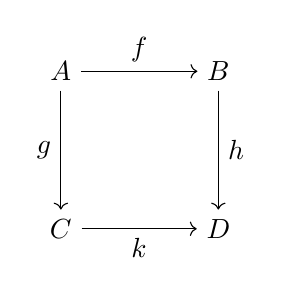
\begin{tikzpicture}
            \node (A) at (0,0) {\(A\)};
            \node (B) at (2,0) {\(B\)};
            \node (C) at (0,-2) {\(C\)};
            \node (D) at (2,-2) {\(D\)};
            \draw[->] (A) -- node[above] {\(f\)} (B);
            \draw[->] (A) -- node[left] {\(g\)} (C);
            \draw[->] (B) -- node[right] {\(h\)} (D);
            \draw[->] (C) -- node[below] {\(k\)} (D);
        \end{tikzpicture}
    \end{center}
    图表交换意味着两点间任意态射合成均相等, 比如 \(h \circ f = k \circ g\).
\end{definition}

\begin{example}
    定义 \(\mathbf{Set}\) 为集合范畴, 其中对象为集合, 对象间态射为映射.
\end{example}

\begin{example}
    定义 \(\mathbf{0}\) 为空范畴, 也即 \(\mathrm{Ob} (\mathbf{0}) = \emptyset\).
\end{example}

\begin{example}
    对偏序集 \(P\), 定义其对应的范畴 \(\mathrm{Cat} (P)\) 如下:

    \begin{enumerate}
        \item 对象是 \(P\) 中的元素.
        \item \(x \leq y\) 时有唯一态射 \(x \to y\).
        \item \(x \nleq y\) 时没有态射.
    \end{enumerate}
\end{example}

\begin{definition}
    对集合 \(S\) 定义离散范畴 \(\mathrm{Disc} (S)\) 如下:

    \begin{enumerate}
        \item 对象是 \(S\) 中的元素.
        \item 仅有单位态射.
    \end{enumerate}
\end{definition}

\begin{definition}
    若有一组映射 \(f : X \to Y\), \(g : Y \to X\) 使得 \(g \circ f = \mathrm{id}_X\), \(f \circ g = \mathrm{id}_Y\), 则称 \(f\) 为 \(g\) 的逆, \(f\) 是同构,
    记作 \(f^{-1} = g\).

    \(X\) 与 \(Y\) 同构记作 \(X \cong Y\), 命全体 \(X\) 与 \(Y\) 间的同构为 \(\mathrm{Isom}_{\mathcal{C}} (X,Y)\).
\end{definition}

\begin{definition}
    定义自同态集 \(\mathrm{End}_{\mathcal{C}} (X) := \mathrm{Hom}_{\mathcal{C}} (X,X)\) 与自同构集
    \(\mathrm{Aut}_{\mathcal{C}} (X) := \mathrm{Isom}_{\mathcal{C}} (X,X)\), 其上有自然的复合运算.
\end{definition}

\begin{definition}
    态射 \(f : X \to Y\) 称为单态射 (monomorphism), 如果对于任意 \(g,h : Z \to X\), 有 \(f \circ g = f \circ h \implies g = h\).

    态射 \(f : X \to Y\) 称为满态射 (epimorphism), 如果对于任意 \(g,h : Y \to Z\), 有 \(g \circ f = h \circ f \implies g = h\).
\end{definition}

\begin{definition}[反范畴]
    定义范畴 \(\mathcal{C}^{\mathrm{op}}\) 如下:

    \begin{enumerate}
        \item \(\mathrm{Ob} (\mathcal{C}^{\mathrm{op}}) = \mathrm{Ob} (\mathcal{C})\).
        \item \(\mathrm{Hom}_{\mathcal{C}^{\mathrm{op}}} (X,Y) = \mathrm{Hom}_{\mathcal{C}} (Y,X)\).
        \item 对于态射 \(f : X \to Y, g : Y \to Z\), 定义 \(g \circ_{\mathrm{op}} f := f \circ g\).
    \end{enumerate}
\end{definition}

\begin{definition}[函子]
    \label {definition:functor}
    一个函子 \(F : \mathcal{C} \to \mathcal{D}\) 包含以下资料:

    \begin{enumerate}
        \item 对象映射 \(F : \mathrm{Ob} (\mathcal{C}) \to \mathrm{Ob} (\mathcal{D})\).
        \item 对于任意对象 \(X,Y \in \mathcal{C}\), 有映射 \(F : \mathrm{Hom}_{\mathcal{C}} (X,Y) \to \mathrm{Hom}_{\mathcal{D}} (F(X),F(Y))\).
        \item 对于任意对象 \(X \in \mathcal{C}\), 映单位态射为单位态射 \(F(\mathrm{id}_X) = \mathrm{id}_{F(X)}\).
        \item 对于任意对象 \(X,Y,Z \in \mathcal{C}\) 保持态射的复合 \(F(g \circ f) = F(g) \circ F(f)\).
    \end{enumerate}
\end{definition}

\begin{definition}[反变函子]
    定义 \(\mathcal{C}\) 出发反变函子为从其反范畴出发的函子.
\end{definition}

\begin{definition}
    一个函子称为忠实 (faithful), 如果对于任意对象 \(X,Y \in \mathcal{C}\), 映射 \(F : \mathrm{Hom}_{\mathcal{C}} (X,Y) \to \mathrm{Hom}_{\mathcal{D}} (F(X),F(Y))\) 是单射.

    一个函子称为全 (full), 如果对于任意对象 \(X,Y \in \mathcal{C}\), 映射 \(F : \mathrm{Hom}_{\mathcal{C}} (X,Y) \to \mathrm{Hom}_{\mathcal{D}} (F(X),F(Y))\) 是满射.

    一个函子称本质满 (essentially surjective), 如果对于任意对象 \(Y \in \mathcal{D}\), 存在对象 \(X \in \mathcal{C}\) 使得 \(F(X) \cong Y\).
\end{definition}

\begin{definition}
    对于函子 \(F : \mathcal{C} \to \mathcal{D}\), \(G : \mathcal{D} \to \mathcal{E}\), 定义函子间的复合 \((G \circ F) (X) := G(F(X))\), \((G \circ F) (f) := G(F(f))\).

    \begin{proof}
        只需注意到 \(G(F(f)) \circ G(F(g)) = G(F(f) \circ F(g)) = G(F(f \circ g))\).
    \end{proof}
\end{definition}

\begin{definition}
    显见函子复合满足结合律, 定义范畴 \(\mathbf{Cat}\) 如下:

    \begin{enumerate}
        \item 对象是 \(\mathrm{Ob} (\mathcal{C}), \mathrm{Mor} (\mathcal{C})\) 是集合的范畴 \(\mathcal{C}\).
        \item \(\mathrm{Hom}_{\mathbf{Cat}} (\mathcal{C},\mathcal{D})\) 是所有函子 \(\mathcal{C} \to \mathcal{D}\).
    \end{enumerate}
\end{definition}

\begin{definition}[自然变换]
    两个函子 \(F,G : \mathcal{C} \to \mathcal{D}\) 之间的自然变换 (natural transformation) \(\eta : F \to G\) 为对所有 \(X \in \mathrm{Ob} (C)\) 择定的态射 \(\eta_X : F(X) \to G(X)\),
    满足对于任意对象 \(X,Y \in \mathcal{C}\) 与 \(f \in \mathrm{Hom}_{\mathcal{C}} (X,Y)\), 有交换图表:
        
    \begin{center}
        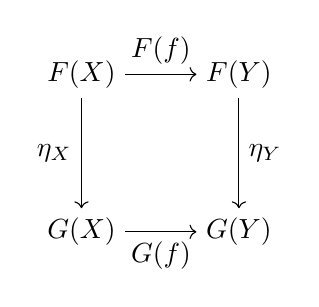
\begin{tikzpicture}
            \node (FX) at (0,0) {\(F(X)\)};
            \node (FY) at (2,0) {\(F(Y)\)};
            \node (GX) at (0,-2) {\(G(X)\)};
            \node (GY) at (2,-2) {\(G(Y)\)};
            \draw[->] (FX) -- node[above] {\(F(f)\)} (FY);
            \draw[->] (FX) -- node[left] {\(\eta_X\)} (GX);
            \draw[->] (FY) -- node[right] {\(\eta_Y\)} (GY);
            \draw[->] (GX) -- node[below] {\(G(f)\)} (GY);
        \end{tikzpicture}
    \end{center}

    记作 \(\eta : F \to G\), 可以画作图表:

    \begin{center}
        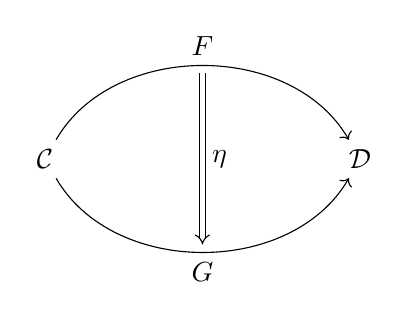
\begin{tikzpicture}
            \node (C) at (-2,0) {\(\mathcal{C}\)};
            \node (D) at (2,0) {\(\mathcal{D}\)};
            \draw[->] (C) to[bend left=60] node[above] (F) {\(F\)} (D);
            \draw[->] (C) to[bend right=60] node[below] (G) {\(G\)} (D);
            \draw[double,-{Implies},double distance = 0.15em] ($(F.south) + (0,- 0.1)$) to node[right] {\(\eta\)} ($(G.north) + (0,0.1)$);
        \end{tikzpicture}
    \end{center}
\end{definition}

\begin{definition}[纵合成]
    给出 \(\eta : F \to G\), \(\theta : G \to H\), 定义纵合成 \(\theta \circ \eta : F \to H\) 为 \({(\theta \circ \eta)}_X := \theta_X \circ \eta_X\), 解作图表:
    
    \[
        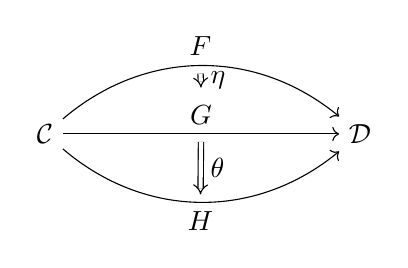
\begin{tikzpicture}
            \node (C) at (-2,0) {\(\mathcal{C}\)};
            \node (D) at (2,0) {\(\mathcal{D}\)};
            \draw[->] (C) to[bend left=40] node[above] (F) {\(F\)} (D);
            \draw[->] (C) to node[above] (G) {\(G\)} (D);
            \draw[->] (C) to[bend right=40] node[below] (H) {\(H\)} (D);
            \draw[double,-{Implies},double distance = 0.15em] ($(F.south) + (0,- 0.1)$) to node[right] {\(\eta\)} ($(G.north) + (0,0.1)$);
            \draw[double,-{Implies},double distance = 0.15em] ($(G.south) + (0,- 0.1)$) to node[right] {\(\theta\)} ($(H.north) + (0,0.1)$);
        \end{tikzpicture} = 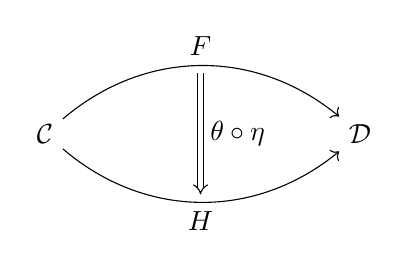
\begin{tikzpicture}
            \node (C) at (-2,0) {\(\mathcal{C}\)};
            \node (D) at (2,0) {\(\mathcal{D}\)};
            \draw[->] (C) to[bend left=40] node[above] (F) {\(F\)} (D);
            \draw[->] (C) to[bend right=40] node[below] (H) {\(H\)} (D);
            \draw[double,-{Implies},double distance = 0.15em] ($(F.south) + (0,- 0.1)$) to node[right] {\(\theta \circ \eta\)} ($(H.north) + (0,0.1)$);
        \end{tikzpicture}
    \]

    \begin{proof}
        只需注意到以下交换图表 (两小方块交换故外框交换):

        \begin{center}
            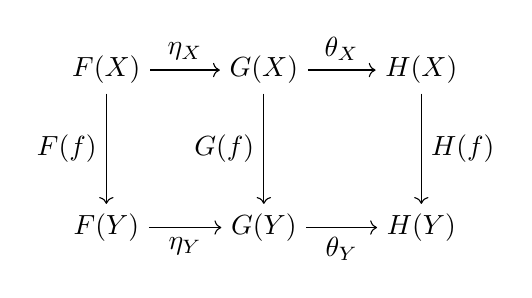
\begin{tikzpicture}
                \node (FX) at (-2,1) {\(F(X)\)};
                \node (FY) at (-2,-1) {\(F(Y)\)};
                \node (GX) at (0,1) {\(G(X)\)};
                \node (GY) at (0,-1) {\(G(Y)\)};
                \node (HX) at (2,1) {\(H(X)\)};
                \node (HY) at (2,-1) {\(H(Y)\)};
                \draw[->] (FX) -- node[left] {\(F(f)\)} (FY);
                \draw[->] (FX) -- node[above] {\(\eta_X\)} (GX);
                \draw[->] (FY) -- node[below] {\(\eta_Y\)} (GY);
                \draw[->] (GX) -- node[left] {\(G(f)\)} (GY);
                \draw[->] (GX) -- node[above] {\(\theta_X\)} (HX);
                \draw[->] (GY) -- node[below] {\(\theta_Y\)} (HY);
                \draw[->] (HX) -- node[right] {\(H(f)\)} (HY);
            \end{tikzpicture}
        \end{center}
    \end{proof}
\end{definition}

\begin{definition}[横合成]
    给出三个范畴 \(\mathcal{C},\mathcal{D},\mathcal{E}\) 以及四个函子 \(F_1,F_2 : \mathcal{C} \to \mathcal{D}\), \(G_1,G_2 : \mathcal{D} \to \mathcal{E}\), 
    给出自然变换 \(\eta : F_1 \to F_2\), \(\theta : G_1 \to G_2\), 定义横合成 \(\theta \ast \eta : G_1 \circ F_1 \to G_2 \circ F_2\) 为 \({(\theta \ast \eta)}_X := \theta_{F_2 (X)} \circ G_1 (\eta_X)\), 解作图表:

    \[
        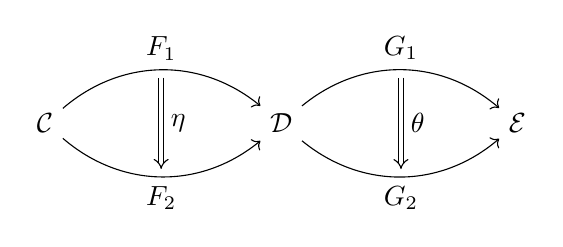
\begin{tikzpicture}
            \node (C) at (-3,0) {\(\mathcal{C}\)};
            \node (D) at (0,0) {\(\mathcal{D}\)};
            \node (E) at (3,0) {\(\mathcal{E}\)};
            \draw[->] (C) to[bend left=40] node[above] (F1) {\(F_1\)} (D);
            \draw[->] (C) to[bend right=40] node[below] (F2) {\(F_2\)} (D);
            \draw[->] (D) to[bend left=40] node[above] (G1) {\(G_1\)} (E);
            \draw[->] (D) to[bend right=40] node[below] (G2) {\(G_2\)} (E);
            \draw[double,-{Implies},double distance = 0.15em] ($(F1.south) + (0,- 0.1)$) to node[right] {\(\eta\)} ($(F2.north) + (0,0.1)$);
            \draw[double,-{Implies},double distance = 0.15em] ($(G1.south) + (0,- 0.1)$) to node[right] {\(\theta\)} ($(G2.north) + (0,0.1)$);
        \end{tikzpicture} = 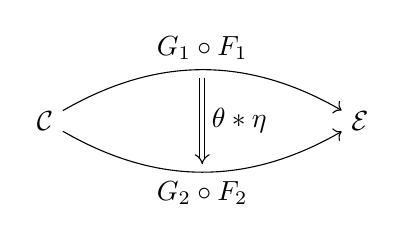
\begin{tikzpicture}
            \node (C) at (-2,0) {\(\mathcal{C}\)};
            \node (E) at (2,0) {\(\mathcal{E}\)};
            \draw[->] (C) to[bend left=30] node[above] (G1F1) {\(G_1 \circ F_1\)} (E);
            \draw[->] (C) to[bend right=30] node[below] (G2F2) {\(G_2 \circ F_2\)} (E);
            \draw[double,-{Implies},double distance = 0.15em] ($(G1F1.south) + (0,- 0.1)$) to node[right] {\(\theta \ast \eta\)} ($(G2F2.north) + (0,0.1)$);
        \end{tikzpicture}
    \]

    \begin{proof}
        需注意到以下交换图表:

        \begin{center}
            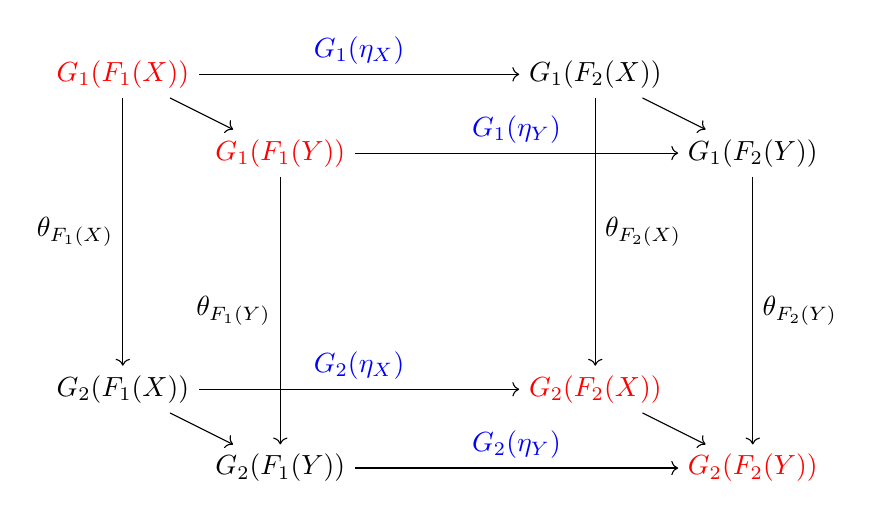
\begin{tikzpicture}
                \node (G1F1X) at (-4,4) {\textcolor{red}{\(G_1 (F_1 (X))\)}};
                \node (G1F1Y) at (-2,3) {\textcolor{red}{\(G_1 (F_1 (Y))\)}};
                \node (G1F2X) at (2,4) {\(G_1 (F_2 (X))\)};
                \node (G1F2Y) at (4,3) {\(G_1 (F_2 (Y))\)};
                \node (G2F1X) at (-4,0) {\(G_2 (F_1 (X))\)};
                \node (G2F1Y) at (-2,-1) {\(G_2 (F_1 (Y))\)};
                \node (G2F2X) at (2,0) {\textcolor{red}{\(G_2 (F_2 (X))\)}};
                \node (G2F2Y) at (4,-1) {\textcolor{red}{\(G_2 (F_2 (Y))\)}};
                \draw[->] (G1F1X) -- (G1F1Y);
                \draw[->] (G1F2X) -- (G1F2Y);
                \draw[->] (G2F1X) -- (G2F1Y);
                \draw[->] (G2F2X) -- (G2F2Y);
                \draw[->] (G1F1X) -- node[above] {\textcolor{blue}{\(G_1 (\eta_X)\)}} (G1F2X);
                \draw[->] (G1F1Y) -- node[above] {\textcolor{blue}{\(G_1 (\eta_Y)\)}} (G1F2Y);
                \draw[->] (G2F1X) -- node[above] {\textcolor{blue}{\(G_2 (\eta_X)\)}} (G2F2X);
                \draw[->] (G2F1Y) -- node[above] {\textcolor{blue}{\(G_2 (\eta_Y)\)}} (G2F2Y);
                \draw[->] (G1F1X) -- node[left] {{\(\theta_{F_1 (X)}\)}} (G2F1X);
                \draw[->] (G1F1Y) -- node[left] {\(\theta_{F_1 (Y)}\)} (G2F1Y);
                \draw[->] (G1F2X) -- node[right] {\(\theta_{F_2 (X)}\)} (G2F2X);
                \draw[->] (G1F2Y) -- node[right] {\(\theta_{F_2 (Y)}\)} (G2F2Y);
            \end{tikzpicture}
        \end{center}

        前后左右四面交换源自 \(\theta\) 为自然变换, 上下两面交换源自 \(\eta\) 为自然变换, 于是\textcolor{red}{红色}标记出的子图亦交换.
    \end{proof}
\end{definition}

特别的, 在标记自然变换时, 我们可以将单独的函子 \(F\) 拉开成为 \(\mathrm{id}_F : F \to F\), 在每个 \(X\) 上为 \(\mathrm{id}_{F(X)}\).

\begin{definition}
    对于范畴 \(\mathcal{C}, \mathcal{D}\), 定义函子范畴 \(\mathbf{Fun} (\mathcal{C},\mathcal{D})\) 如下:

    \begin{enumerate}
        \item 对象是函子 \(\mathcal{C} \to \mathcal{D}\).
        \item 对于函子 \(F,G : \mathcal{C} \to \mathcal{D}\), 定义态射集 \(\mathrm{Hom}_{\mathbf{Fun} (\mathcal{C},\mathcal{D})} (F,G)\) 为所有 \(F \to G\) 的自然变换.
        \item 态射的合成是自然变换的纵合成.
    \end{enumerate}

    \begin{proof}
        只需证明纵合成之结合律, 只需注意到态射结合律:

        \[
            (\theta_X \circ \eta_X) \circ \phi_X = \theta_X \circ (\eta_X \circ \phi_X)
        \]
    \end{proof}
\end{definition}

\begin{lemma}
    函子的纵合成满足结合律.

    \begin{proof}
        给出自然变换 \(\theta, \psi, \phi\) 如下:

        \begin{center}
            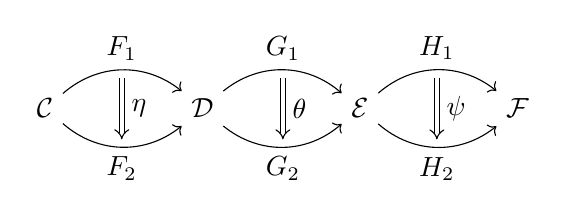
\begin{tikzpicture}
                \node (C) at (-3,0) {\(\mathcal{C}\)};
                \node (D) at (-1,0) {\(\mathcal{D}\)};
                \node (E) at (1,0) {\(\mathcal{E}\)};
                \node (F) at (3,0) {\(\mathcal{F}\)};
                \draw[->] (C) to[bend left=40] node[above] (F1) {\(F_1\)} (D);
                \draw[->] (C) to[bend right=40] node[below] (F2) {\(F_2\)} (D);
                \draw[->] (D) to[bend left=40] node[above] (G1) {\(G_1\)} (E);
                \draw[->] (D) to[bend right=40] node[below] (G2) {\(G_2\)} (E);
                \draw[->] (E) to[bend left=40] node[above] (H1) {\(H_1\)} (F);
                \draw[->] (E) to[bend right=40] node[below] (H2) {\(H_2\)} (F);
                \draw[double,-{Implies},double distance = 0.15em] ($(F1.south) + (0,- 0.1)$) to node[right] {\(\eta\)} ($(F2.north) + (0,0.1)$);
                \draw[double,-{Implies},double distance = 0.15em] ($(G1.south) + (0,- 0.1)$) to node[right] {\(\theta\)} ($(G2.north) + (0,0.1)$);
                \draw[double,-{Implies},double distance = 0.15em] ($(H1.south) + (0,- 0.1)$) to node[right] {\(\psi\)} ($(H2.north) + (0,0.1)$);
            \end{tikzpicture}
        \end{center}

        有交换图表 (交换性源自于施 \(\psi\) 自然性于 \(G_2 \eta_X\)):

        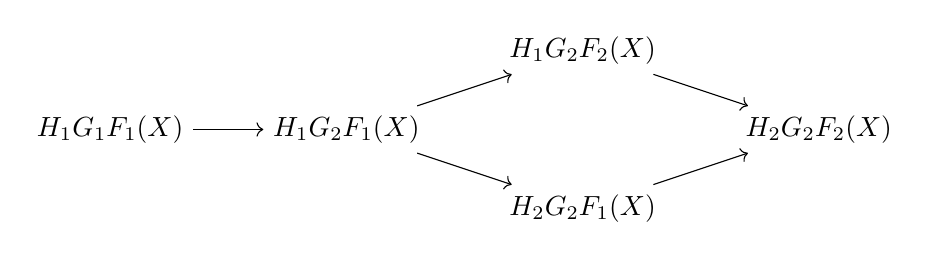
\begin{tikzpicture}
            \node (H1G1F1) at (-4.5,0) {\(H_1 G_1 F_1 (X)\)};
            \node (H1G2F1) at (-1.5,0) {\(H_1 G_2 F_1 (X)\)};
            \node (H1G2F2) at (1.5,1) {\(H_1 G_2 F_2 (X)\)};
            \node (H2G2F2) at (4.5,0) {\(H_2 G_2 F_2 (X)\)};
            \node (H2G2F1) at (1.5,-1) {\(H_2 G_2 F_1 (X)\)};
            \draw[->] (H1G1F1) -- (H1G2F1);
            \draw[->] (H1G2F1) -- (H1G2F2);
            \draw[->] (H1G2F2) -- (H2G2F2);
            \draw[->] (H1G2F1) -- (H2G2F1);
            \draw[->] (H2G2F1) -- (H2G2F2);
        \end{tikzpicture}
    \end{proof}
\end{lemma}

\begin{lemma}
    函子的横纵合成交换, 即亦给出自然变换如下:

    \begin{center}
        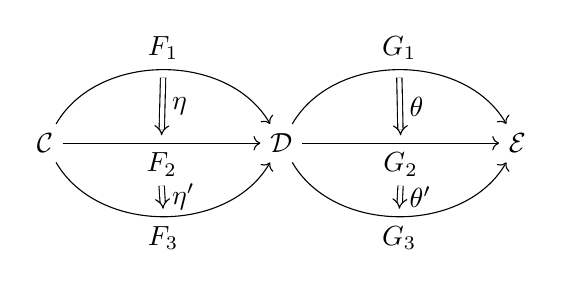
\begin{tikzpicture}
            \node (C) at (-3,0) {\(\mathcal{C}\)};
            \node (D) at (0,0) {\(\mathcal{D}\)};
            \node (E) at (3,0) {\(\mathcal{E}\)};
            \draw[->] (C) to[bend left=60] node[above] (F1) {\(F_1\)} (D);
            \draw[->] (C) to node[below] (F2) {\(F_2\)} (D);
            \draw[->] (C) to[bend right=60] node[below] (F3) {\(F_3\)} (D);
            \draw[->] (D) to[bend left=60] node[above] (G1) {\(G_1\)} (E);
            \draw[->] (D) to node[below] (G2) {\(G_2\)} (E);
            \draw[->] (D) to[bend right=60] node[below] (G3) {\(G_3\)} (E);
            \draw[double,-{Implies},double distance = 0.15em] ($(F1.south) + (0,- 0.1)$) to node[right] {\(\eta\)} ($(F2.north) + (0,0.1)$);
            \draw[double,-{Implies},double distance = 0.15em] ($(F2.south)$) to node[right] {\(\eta^\prime\)} ($(F3.north) + (0,0.1)$);
            \draw[double,-{Implies},double distance = 0.15em] ($(G1.south) + (0,- 0.1)$) to node[right] {\(\theta\)} ($(G2.north) + (0,0.1)$);
            \draw[double,-{Implies},double distance = 0.15em] ($(G2.south)$) to node[right] {\(\theta^\prime\)} ($(G3.north) + (0,0.1)$);
        \end{tikzpicture}
    \end{center}

    则有等式 \((\theta^\prime \ast \eta^\prime) \circ (\theta \ast \eta) = (\theta^\prime \circ \theta) \ast (\eta^\prime \circ \eta)\).

    \begin{proof}
        只需注意到以下交换图表:

        \begin{center}
            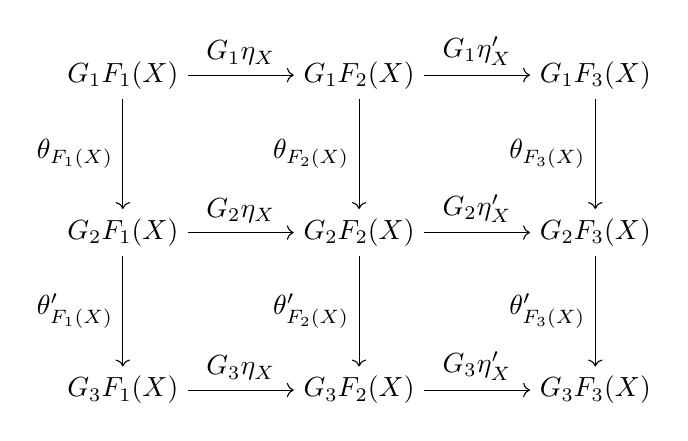
\begin{tikzpicture}
                \node (G1F1X) at (-3,2) {\(G_1 F_1 (X)\)};
                \node (G1F2X) at (0,2) {\(G_1 F_2 (X)\)};
                \node (G1F3X) at (3,2) {\(G_1 F_3 (X)\)};
                \node (G2F1X) at (-3,0) {\(G_2 F_1 (X)\)};
                \node (G2F2X) at (0,0) {\(G_2 F_2 (X)\)};
                \node (G2F3X) at (3,0) {\(G_2 F_3 (X)\)};
                \node (G3F1X) at (-3,-2) {\(G_3 F_1 (X)\)};
                \node (G3F2X) at (0,-2) {\(G_3 F_2 (X)\)};
                \node (G3F3X) at (3,-2) {\(G_3 F_3 (X)\)};
                \draw[->] (G1F1X) to node[above] {\(G_1 \eta_X\)} (G1F2X);
                \draw[->] (G1F2X) to node[above] {\(G_1 \eta^\prime_X\)} (G1F3X);
                \draw[->] (G2F1X) to node[above] {\(G_2 \eta_X\)} (G2F2X);
                \draw[->] (G2F2X) to node[above] {\(G_2 \eta^\prime_X\)} (G2F3X);
                \draw[->] (G3F1X) to node[above] {\(G_3 \eta_X\)} (G3F2X);
                \draw[->] (G3F2X) to node[above] {\(G_3 \eta^\prime_X\)} (G3F3X);
                \draw[->] (G1F1X) to node[left] {\(\theta_{F_1 (X)}\)} (G2F1X);
                \draw[->] (G1F2X) to node[left] {\(\theta_{F_2 (X)}\)} (G2F2X);
                \draw[->] (G1F3X) to node[left] {\(\theta_{F_3 (X)}\)} (G2F3X);
                \draw[->] (G2F1X) to node[left] {\(\theta^\prime_{F_1 (X)}\)} (G3F1X);
                \draw[->] (G2F2X) to node[left] {\(\theta^\prime_{F_2 (X)}\)} (G3F2X);
                \draw[->] (G2F3X) to node[left] {\(\theta^\prime_{F_3 (X)}\)} (G3F3X);
            \end{tikzpicture}
        \end{center}

        每个小正方形交换源于 \(\theta, \theta^\prime\) 为自然变换, 故外框交换.
    \end{proof}
\end{lemma}

\begin{lemma}
    \label {lemma:natural transformation is isomorphism iff each component is isomorphism}
    自然变换 \(\eta : F \to G\) 是同构当且仅当对于任意 \(X \in \mathcal{C}\), \(\eta_X\) 是同构,
    其逆为 \(\eta^{-1} : G \to F\), \(\eta^{-1}_X := {\eta_X}^{-1}\).

    \begin{proof}
        给出其逆业已给出每个 \(\eta_X\) 之逆, 而 \(\eta^{-1}\) 是自然性对应了
        \(\eta\) 自然性的交换图表, 换言之, 以下图表每一小块交换故外框交换.

        \begin{center}
            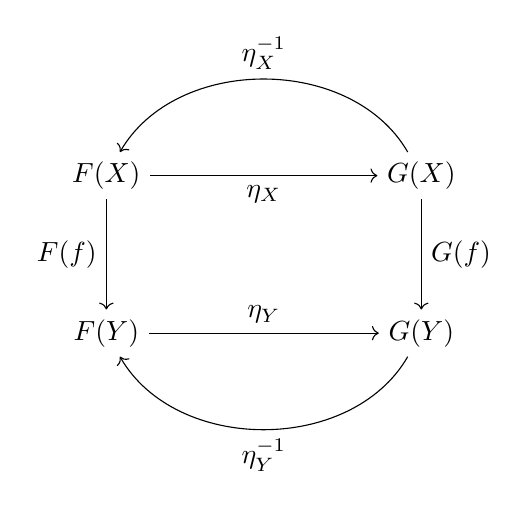
\begin{tikzpicture}
                \node (FX) at (-2,1) {\(F(X)\)};
                \node (FY) at (-2,-1) {\(F(Y)\)};
                \node (GX) at (2,1) {\(G(X)\)};
                \node (GY) at (2,-1) {\(G(Y)\)};
                \draw[->] (FX) to node[left] {\(F(f)\)} (FY);
                \draw[->] (FX) to node[below] {\(\eta_X\)} (GX);
                \draw[->] (FY) to node[above] {\(\eta_Y\)} (GY);
                \draw[->] (GX) to node[right] {\(G(f)\)} (GY);
                \draw[->] (GX) to [bend right=60] node[above] {\(\eta^{-1}_X\)} (FX);
                \draw[->] (GY) to [bend left=60] node[below] {\(\eta^{-1}_Y\)} (FY);
            \end{tikzpicture}
        \end{center}
    \end{proof}
\end{lemma}

\begin{definition}[范畴等价]
    若存在函子 \(F : \mathcal{C} \to \mathcal{D}\), \(G : \mathcal{D} \to \mathcal{C}\) 使得 \(G \circ F \cong \mathrm{id}_{\mathcal{C}}\), \(F \circ G \cong \mathrm{id}_{\mathcal{D}}\), 则称 \(\mathcal{C}\) 与 \(\mathcal{D}\) 等价.

    假定上述定义中 \(\cong\) 为 \(=\), 则称 \(\mathcal{C}\) 与 \(\mathcal{D}\) 同构.
\end{definition}

\begin{definition}[子范畴]
    给定范畴 \(\mathcal{C}^\prime, \mathcal{C}\), 若 \(\mathrm{Ob} (\mathcal{C}^\prime) \subseteq \mathrm{Ob} (\mathcal{C})\), 
    \(\mathrm{Hom}_{\mathcal{C}^\prime} (X,Y) \subseteq \mathrm{Hom}_{\mathcal{C}} (X,Y)\), 且保持复合运算,
    则称 \(\mathcal{C}^\prime\) 是 \(\mathcal{C}\) 的子范畴 (subcategory), 子范畴对应一个自然的嵌入 \(\iota : \mathcal{C}^\prime \to \mathcal{C}\),
    总是忠实, 子范畴亦有全和本质满的性质.
\end{definition}

\begin{definition}[骨架]
    如果范畴 \(\mathcal{C}^\prime\) 是 \(\mathcal{C}\) 的全子范畴, 且对于任意 \(X \in \mathrm{Ob} (\mathcal{C})\),
    都存在唯一 \(X^\prime \in \mathrm{Ob} (\mathcal{C}^\prime)\) 使得 \(X \cong X^\prime\), 则称 \(\mathcal{C}^\prime\) 是 \(\mathcal{C}\) 的骨架 (skeleton).

    自身是骨架的范畴称为骨架范畴 (skeletal category).
\end{definition}

\begin{definition}[小范畴]
    为了避免一些集合论的困难, 我们定义小范畴 (small category) 为态射类是集合的范畴.

    给出一个 Grothendieck 宇宙 \(\mathcal{U}\), 定义 \(\mathcal{U}\)-小范畴为对象类是 \(\mathcal{U}\) 中的集合的范畴.
\end{definition}

\begin{lemma}
    任何小范畴 \(\mathcal{C}\) 有骨架, 且骨架范畴与 \(\mathcal{C}\) 等价.

    \begin{proof}
        注意到 \(\cong\) 显见的是 \(\mathrm{Ob} (\mathcal{C})\) 上的等价关系, 在每个等价类
        上使用 \ref{axiom:NBG Axiom of Choice} 选取代表元 \(X^\prime\), 与等价类中任意一 \(X\) 与 \(X^\prime\) 间同构 \(f_X : X \to X^\prime\),
        选取子范畴 \(\mathcal{C}^\prime\) 如下:

        \begin{enumerate}
            \item 对象集为全体代表元 \(X^\prime\).
            \item 对于任意 \(X^\prime,Y^\prime \in \mathrm{Ob} (\mathcal{C}^\prime)\), \(\mathrm{Hom}_{\mathcal{C}^\prime} (X^\prime,Y^\prime) = \mathrm{Hom}_{\mathcal{C}} (X^\prime,Y^\prime) \).
        \end{enumerate}

        定义 \(\iota^{-1}\) 映 \(X\) 为其代表元 \(X^\prime\), 映 \(f \in \mathrm{Hom}_{\mathcal{C}} (X,Y)\) 为 
        \(f_Y \circ f \circ {f_X}^{-1}\).

        \(\iota^{-1}\) 函子性, \(\iota \circ \iota^{-1} = \mathrm{id}_{\mathcal{C}}\) 是显然的, 而构造 \(\iota^{-1} \circ \iota \cong \mathrm{id}_{\mathcal{C}^\prime}\) 的自然变换为 \(f\) 即可.
    \end{proof}
\end{lemma}

\begin{lemma}
    范畴等价具有传递性.

    \begin{proof}
        给出范畴 \(\mathcal{C},\mathcal{D},\mathcal{E}\), 函子 \(F : \mathcal{C} \to \mathcal{D}\), \(G : \mathcal{D} \to \mathcal{E}\), 
        以及其逆, 给出可逆的自然变换 \(\eta : F \circ F^{-1} \to \mathrm{id}_{\mathcal{D}}\), \(\theta : F^{-1} \circ F \to \mathrm{id}_{\mathcal{C}}\),
        \(\eta^\prime : G \circ G^{-1} \to \mathrm{id}_{\mathcal{E}}\), \(\theta^\prime : G^{-1} \circ G \to \mathrm{id}_{\mathcal{D}}\), 构造自然变换
        \(\eta^\prime \circ (\mathrm{id}_G \ast \eta \ast \mathrm{id}_{G^{-1}}) : G \circ F \circ F^{-1} \circ G^{-1} \to \mathrm{id}_{\mathcal{E}}\) 有逆
        \((\mathrm{id}_G \ast \eta^{-1} \ast \mathrm{id}_{G^{-1}}) \circ {\eta^{\prime}}^{-1}\),  \(\theta\) 侧可同理构造.
    \end{proof}
\end{lemma}

\begin{lemma}
    骨架范畴间的全忠实本质满函子都是同构.

    \begin{proof}
        本质满则在对象集上是双射, 全忠实亦给出每个态射集上的双射.
    \end{proof}
\end{lemma}

\begin{lemma}
    小范畴间函子 \(F\) 是等价当且仅当 \(F\) 全忠实本质满.

    \begin{proof}
        易得骨架范畴间的同构, 考虑等价的传递性即可.
    \end{proof}
\end{lemma}

\subsection{Hom 函子与泛性质}

\begin{definition}
    对于集合 \(I\) 与小范畴 \({(\mathcal{C}_i)}_{i \in I}\), 定义积范畴 \(\prod_{i \in I} \mathcal{C}_i\) 如下:

    \begin{enumerate}
        \item 对象是积 \(\prod_{i \in I} \mathrm{Ob} (\mathcal{C}_i)\) 的元素.
        \item 对于对象 \((X_i)_{i \in I}\), \((Y_i)_{i \in I}\), 定义态射集 \(\mathrm{Hom}_{\prod_{i \in I} \mathcal{C}_i} ((X_i)_{i \in I},(Y_i)_{i \in I})\) 为态射集之积
                \(\prod_{i \in I} \mathrm{Hom}_{\mathcal{C}_i} (X_i,Y_i)\).
        \item 态射的合成是逐点的, 也即 \({(f_i)}_{i \in I} \circ {(g_i)}_{i \in I} = {(f_i \circ g_i)}_{i \in I}\).
    \end{enumerate}

    定义余积范畴 \(\coprod_{i \in I} \mathcal{C}_i\) 如下:

    \begin{enumerate}
        \item 对象是无交并 \(\coprod_{i \in I} \mathrm{Ob} (\mathcal{C}_i)\) 的元素.
        \item 对象 \(X,Y\) 间有态射当且仅当其对应同一个 \(\mathcal{C}_i\), 态射集继承自 \(\mathcal{C}_i\).
    \end{enumerate}

    定义自明的投影函子 \(\mathbf{Pr}_j : \prod_{i \in I} \mathcal{C}_i \to \mathcal{C}_j\) 与包含函子 \(\mathbf{In}_j : \mathcal{C}_j \to \coprod_{i \in I} \mathcal{C}_i\).
\end{definition}

\begin{definition}
    多元函子即为从积范畴出发的函子.
\end{definition}

\begin{definition}[Hom 函子]
    对于任意范畴 \(\mathcal{C}\), 有函子 \(\mathrm{Hom}_{\mathcal{C}} (-,-) : \mathcal{C}^{\mathrm{op}} \times \mathcal{C} \to \mathbf{Set}\), 映 \((X,Y)\) 为态射集 \(\mathrm{Hom}_{\mathcal{C}} (X,Y)\), 
    映 \(\mathcal{C}^{\mathrm{op}} \times \mathcal{C}\) 中态射 \((f,g)\) 为映射 \(\phi \mapsto g \circ \phi \circ f\).

    称 \(\phi\) 对 \(f\) 做拉回 (pullback), 对 \(g\) 做推出 (pushforward).
\end{definition}

\begin{lemma}
    存在自然同构 \({(\mathbf{Fun} (\mathcal{C}_1 ,\mathcal{C}_2))}^\mathrm{op} \cong \mathbf{Fun} ({\mathcal{C}_1}^\mathrm{op}, {\mathcal{C}_2}^\mathrm{op})\).
\end{lemma}

\begin{lemma}
    有恒等式 \(\mathbf{Fun} (\mathrm{Disc} (I), \mathcal{C}) \cong \prod_{i \in I} \mathcal{C}\).
\end{lemma}

\begin{definition}[中心]
    一个范畴的中心定义为 \(\mathrm{Z} (\mathcal{C}) := \mathrm{End} (\mathrm{id}_{\mathcal{C}})\).

    对范畴等价 \(F : \mathcal{C} \to \mathcal{D}\), 诱导出中心的同构 \(\mathrm{Z} (\mathcal{C}) \cong \mathrm{Z} (\mathcal{D})\).
\end{definition}

\begin{definition}
    假设范畴 \(\mathcal{C}\) 中对象 \(X\) 满足任意 \(Y \in \mathrm{Ob} (\mathcal{C})\), \(\mathrm{Hom}_{\mathcal{C}} (X,Y)\) 是单点集, 则称 \(X\) 是始对象 (initial object).
    对称的 \(\mathrm{Hom}_{\mathcal{C}} (Y,X)\) 是单点集的对象称为终对象 (terminal object).既是始对象又是终对象的对象称为零对象 (zero object).
\end{definition}

\begin{example}
    在 \(\mathbf{Set}\) 中, 空集是始对象, 任意单点集是终对象.
\end{example}

\begin{definition}
    始对象间有唯一的同构, 终对象亦然.

    \begin{proof}
        给出始对象 \(X,Y\), 存在唯一的 \(f : X \to Y\), \(g : Y \to X\),
        同样存在唯一的 \(\mathrm{id}_X : X \to X\), \(\mathrm{id}_Y : Y \to Y\), 于是 \(f \circ g = \mathrm{id}_Y\), \(g \circ f = \mathrm{id}_X\).

        终对象只需注意到任意 \(\mathcal{C}\) 的终对象都是 \(\mathcal{C}^{\mathrm{op}}\) 的始对象.
    \end{proof}
\end{definition}

\begin{definition}
    泛性质 (universal property) 是一种在某个范畴下是始对象或终对象的性质, 其有自然的唯一性.
\end{definition}

\begin{definition}[图范畴]
    给出一个图表样式, 定义该图的范畴如下:

    \begin{enumerate}
        \item 对象是所有使得图表交换的一种填涂方式.
        \item 态射是相同位置的对象逐点的态射, 满足生成的柱状图表交换.
    \end{enumerate}
\end{definition}

\begin{example}[态射范畴]
    称下图的图范畴为 \(\mathcal{C}\) 的态射范畴:

    \begin{center}
        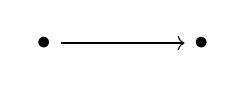
\begin{tikzpicture}
            \node (P1) at (-1,0) {\(\bullet\)};
            \node (P2) at (1,0) {\(\bullet\)};
            \draw[->] (P1) to (P2);
        \end{tikzpicture}
    \end{center}

    即对象是 \(\mathcal{C}\) 中两个对象 \(A,B\) 和一个态射 \(f : A \to B\), 由于确定 \(f\) 亦确定了 \(A,B\),
    也可将对象解作 \(\mathcal{C}\) 中的映射, \(f_1,f_2\) 间的态射是满足以下图表交换的 \((\phi_A, \phi_B)\):

    \begin{center}
        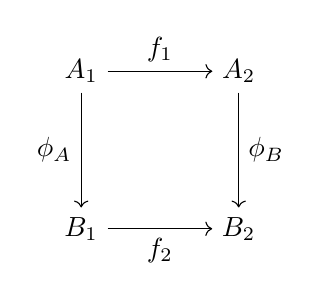
\begin{tikzpicture}
            \node (A1) at (-1,1) {\(A_1\)};
            \node (A2) at (1,1) {\(A_2\)};
            \node (B1) at (-1,-1) {\(B_1\)};
            \node (B2) at (1,-1) {\(B_2\)};
            \draw[->] (A1) to node[above] {\(f_1\)} (A2);
            \draw[->] (B1) to node[below] {\(f_2\)} (B2);
            \draw[->] (A1) to node[left] {\(\phi_A\)} (B1);
            \draw[->] (A2) to node[right] {\(\phi_B\)} (B2);
        \end{tikzpicture}
    \end{center}
\end{example}

\begin{example}[逗号范畴]
    给出函子 \(S : \mathcal{A} \to \mathcal{C}\), \(T : \mathcal{B} \to \mathcal{C}\), 定义逗号范畴 \((S / T)\) 为下图的图范畴:

    \begin{center}
        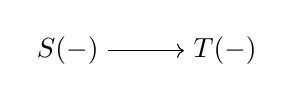
\begin{tikzpicture}
            \node (S) at (-1,0) {\(S (-)\)};
            \node (T) at (1,0) {\(T (-)\)};
            \draw[->] (S) to (T);
        \end{tikzpicture}
    \end{center}

    解作对象是 \(\mathcal{A}\) 中的对象 \(A\), \(\mathcal{B}\) 中的对象 \(B\), 以及 \(\mathcal{C}\) 中的态射 \(f : S(A) \to T(B)\) 组成的 \((A,B,f)\),
    一个 \((A,B,f)\) 到 \((A^\prime,B^\prime,f^\prime)\) 的态射是一对态射 \(g : A \to A^\prime\) 与 \(h : B \to B^\prime\) 使得下图交换:

    \begin{center}
        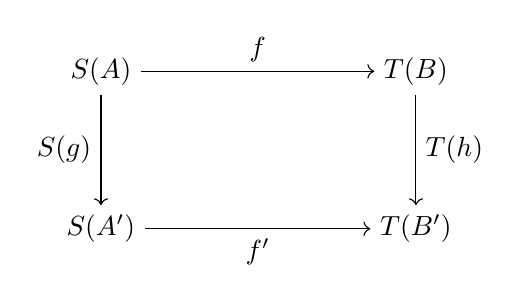
\begin{tikzpicture}
            \node (SA) at (-2,1) {\(S(A)\)};
            \node (TB) at (2,1) {\(T(B)\)};
            \node (SAP) at (-2,-1) {\(S(A^\prime)\)};
            \node (TBP) at (2,-1) {\(T(B^\prime)\)};
            \draw[->] (SA) to node[above] {\(f\)} (TB);
            \draw[->] (SAP) to node[below] {\(f^\prime\)} (TBP);
            \draw[->] (SA) to node[left] {\(S(g)\)} (SAP);
            \draw[->] (TB) to node[right] {\(T(h)\)} (TBP);
        \end{tikzpicture}
    \end{center}
\end{example}

\begin{definition}[子对象, 商对象]
    对 \(X \in \mathrm{Ob} (\mathcal{C})\), 定义 \(X\) 的子对象为单态射 \(i : Y \to X\),
    定义商对象为满态射 \(p : X \to Z\), 在子对象和商对象上定义序:

    定义子对象与商对象的范畴:

    \begin{enumerate}
        \item 对象是 \(X\) 的子对象.
        \item \(i_1 : Y_1 \to X\) 与 \(i_2 : Y_2 \to X\) 的态射是 \(f : Y_1 \to Y_2\) 使得 \(i_1 = i_2 \circ f\).
    \end{enumerate}

    \begin{enumerate}
        \item 对象是 \(X\) 的商对象.
        \item \(p_1 : X \to Z_1\) 与 \(p_2 : X \to Z_2\) 的态射是 \(f : Z_1 \to Z_2\) 使得 \(p_1 = f \circ p_2\).
    \end{enumerate}

    定义子对象与商对象的偏序: \(i_1 \le i_2\) 当且仅当有子对象范畴中的态射 \(f : Y_1 \to Y_2\),
    \(p_1 \le p_2\) 当且仅当有商对象范畴中的态射 \(f : Z_1 \to Z_2\).
\end{definition}

\begin{lemma}
    如果子对象 \(i_1 \le i_2\) 且 \(i_2 \le i_1\), 则子对象 \(i_1\) 与 \(i_2\) 同构, 商对象亦然.

    \begin{proof}
        注意到两个子对象间存在态射则唯一, 于是两个方向均合成为恒等态射.

        商对象无非是 \(\mathcal{C}^{\mathrm{op}}\) 中的子对象.
    \end{proof}
\end{lemma}

\subsection{米田引理}

\begin{definition}[预层]
    给出小范畴 \(\mathcal{C}\), 定义范畴 \(\mathcal{C}^{\vee} : \mathbf{Fun} (\mathcal{C}^{\mathrm{op}}, \mathbf{Set}^{\mathrm{op}})\) 与
    \(\mathcal{C}^{\wedge} : \mathbf{Fun} (\mathcal{C}^{\mathrm{op}}, \mathbf{Set})\), 称 \(\mathcal{C}^{\wedge}\) 为预层 (presheaf) 范畴.
\end{definition}

\begin{definition}
    我们可以自然的将 \(\mathcal{C}\) 嵌入 \(\mathcal{C}^{\wedge}\) 如下:
    \[
        h_{\mathcal{C}} : S \mapsto \mathrm{Hom}_{\mathcal{C}} (-,S)
    \]
    定义自然的求值函子 \(\mathrm{ev}^{\wedge} : \mathcal{C}^{\mathrm{op}} \times \mathcal{C}^{\wedge} \to \mathbf{Set}\) 如下:
    \[
        \mathrm{ev}^{\wedge} (X,S) := S(X)
    \]
    对偶的, 定义 \(k_\mathcal{C} : \mathcal{C} \to \mathcal{C}^{\vee}, \mathrm{ev}^{\vee} : {(\mathcal{C}^{\vee})}^{\mathrm{op}} \times \mathcal{C} \to \mathbf{Set}\) 如下:
    \[
        k_\mathcal{C} (S) := \mathrm{Hom}_{\mathcal{C}} (S,-), \mathrm{ev}^{\vee} (S,X) := S(X)
    \]
\end{definition}

下述引理称米田引理 (Yoneda lemma), 是范畴论中非常重要的引理.

\begin{lemma}[Yoneda]
    \setlabel {米田引理}
    \label {lemma:Yoneda lemma}
    对于任意 \(\mathcal{C}\) 上的预层 \(A \in \mathrm{Ob} (\mathcal{C}^{\wedge})\), 与对象 \(S \in \mathcal{C}\), 
    存在 \(\mathrm{Hom}_{\mathcal{C}^{\wedge}} (h_{\mathcal{C}} (S), A) \cong A(S)\) 的自然双射:
    \[
        (\phi : h_{\mathcal{C}} (S) \to A) \mapsto \phi_S (\mathrm{id}_S)
    \]
    此双射给出 \(\mathrm{Hom}_{\mathcal{C}^{\wedge}} (h_{\mathcal{C}} (-), -)\) 与 \(\mathrm{ev}^{\wedge}\) 的同构.

    \begin{proof}
        证明的技巧在于向层的嵌入将映射转为拉回和推出, 所以对于所有 \(a \in A(S)\), 可以限制出 \(\phi_a : h_{\mathcal{C}} (S) \to A\) 为 \(f \in \mathrm{Hom}_{\mathcal{C}} (X,S)\) 有:
        \[
            \phi_a (f) = \phi_a (\mathrm{id}_S \circ f) = \phi_a (((h_{\mathcal{C}} (S)) (f)) (\mathrm{id}_S)) = A(f) \phi_a (\mathrm{id}_S) = A(f) (a)
        \]
        \begin{center}
            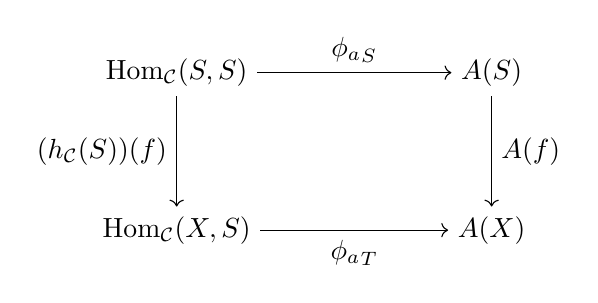
\begin{tikzpicture}
                \node (HSS) at (-2,1) {\(\mathrm{Hom}_{\mathcal{C}} (S,S)\)};
                \node (HXS) at (-2,-1) {\(\mathrm{Hom}_{\mathcal{C}} (X,S)\)};
                \node (AS) at (2,1) {\(A(S)\)};
                \node (AX) at (2,-1) {\(A(X)\)};
                \draw[->] (HSS) to node[left] {\((h_{\mathcal{C}} (S)) (f)\)} (HXS);
                \draw[->] (AS) to node[right] {\(A(f)\)} (AX);
                \draw[->] (HSS) to node[above] {\({\phi_a}_S\)} (AS);
                \draw[->] (HXS) to node[below] {\({\phi_a}_T\)} (AX);
            \end{tikzpicture}
        \end{center}

        自然性展开符号即可, 同构基于 \ref{lemma:natural transformation is isomorphism iff each component is isomorphism}.
    \end{proof}
\end{lemma}

\begin{lemma}
    上述 \(h_\mathcal{C}\) 是全忠实函子, 给出了自然的嵌入 \(\mathcal{C} \to \mathcal{C}^{\wedge}\).

    \begin{proof}
        全忠实性考虑取 \(A\) 为 \(h_\mathcal{C}(T)\), \ref{lemma:Yoneda lemma} 即给出 \(\mathrm{Hom}_{\mathcal{C}^{\wedge}} (h_{\mathcal{C}} (S), h_{\mathcal{C}} (T))\), \(\mathrm{Hom}_{\mathcal{C}} (S,T)\)
        间双射.
    \end{proof}
\end{lemma}

\begin{corollary}
    对称的, \(k_\mathcal{C}\) 全忠实, 且有自然的函子同构 \(\mathrm{Hom}_{\mathcal{C}^{\vee}} (k_{\mathcal{C}} (-), -) \to \mathrm{ev}^{\vee}\).

    \begin{proof}
        只需注意到恒等式 \({(\mathcal{C}^{\vee})}^\mathrm{op} = {(\mathcal{C}^{\mathrm{op}})}^{\wedge}\).
    \end{proof}
\end{corollary}

\begin{definition}[可表]
    称预层 \(A\) 可表 (representable) 当且仅当存在对象 \(S \in \mathcal{C}\) 并给出 \(A \cong h_{\mathcal{C}} (S)\) 的同构 \(\phi : h_{\mathcal{C}} (S) \to A\),
    并称 \((S,\phi)\) 是 \(A\) 的代表元, 对 \(B \in \mathbf{Fun} (\mathcal{C},\mathbf{Set})\) 亦然.
\end{definition}

\begin{lemma}
    代表元若存在则在同构意义下唯一.

    \begin{proof}
        利用米田嵌入的全忠实性.
    \end{proof}
\end{lemma}

\subsection{伴随对}

\begin{definition}[伴随]
    给出函子 \(F : \mathcal{C} \to \mathcal{D}\), \(G : \mathcal{D} \to \mathcal{C}\), 
    与自然变换 \(\eta : \mathrm{id}_{\mathcal{C}} \to G \circ F\), \(\varepsilon : F \circ G \to \mathrm{id}_{\mathcal{D}}\),
    使得以下两图表合成为恒等自然变换:

    \begin{center}
        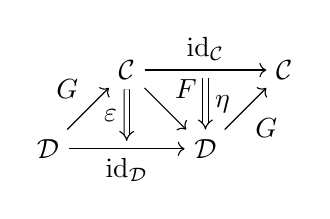
\begin{tikzpicture}
            \node (C1) at (-0.5,0.5) {\(\mathcal{C}\)};
            \node (C2) at (1.5,0.5) {\(\mathcal{C}\)};
            \node (D1) at (-1.5,-0.5) {\(\mathcal{D}\)};
            \node (D2) at (0.5,-0.5) {\(\mathcal{D}\)};
            \draw[->] (C1) to node[above] (idc) {\(\mathrm{id}_{\mathcal{C}}\)} (C2);
            \draw[->] (D1) to node[below] (idd) {\(\mathrm{id}_{\mathcal{D}}\)} (D2);
            \draw[->] (D1) to node[above left] {\(G\)} (C1);
            \draw[->] (D2) to node[below right] {\(G\)} (C2);
            \draw[->] (C1) to node[above right] {\(F\)} (D2);
            \draw[-{Implies},double,double distance = 0.15em] (C1) to node[left] {\(\varepsilon\)} ($(idd.north) + (0,0.1)$);
            \draw[-{Implies},double,double distance = 0.15em] ($(idc.south) + (0,-0.1)$) to node[right] {\(\eta\)} (D2);
        \end{tikzpicture} 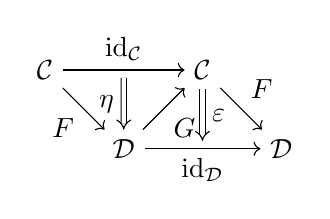
\begin{tikzpicture}
            \node (C1) at (-1.5,0.5) {\(\mathcal{C}\)};
            \node (C2) at (0.5,0.5) {\(\mathcal{C}\)};
            \node (D1) at (-0.5,-0.5) {\(\mathcal{D}\)};
            \node (D2) at (1.5,-0.5) {\(\mathcal{D}\)};
            \draw[->] (C1) to node[above] (idc) {\(\mathrm{id}_{\mathcal{C}}\)} (C2);
            \draw[->] (D1) to node[below] (idd) {\(\mathrm{id}_{\mathcal{D}}\)} (D2);
            \draw[->] (C1) to node[below left] {\(F\)} (D1);
            \draw[->] (C2) to node[above right] {\(F\)} (D2);
            \draw[->] (D1) to node[below right] {\(G\)} (C2);
            \draw[-{Implies},double,double distance = 0.15em] (C2) to node[right] {\(\varepsilon\)} ($(idd.north) + (0,0.1)$);
            \draw[-{Implies},double,double distance = 0.15em] ($(idc.south) + (0,-0.1)$) to node[left] {\(\eta\)} (D1);
        \end{tikzpicture}
    \end{center}

    写成合成为:

    \[
        (\mathrm{id}_{G} \ast \varepsilon) \circ (\eta \ast \mathrm{id}_{G}) = \mathrm{id}_{G}, (\varepsilon \ast \mathrm{id}_{F}) \circ (\mathrm{id}_{F} \ast \eta) = \mathrm{id}_{F}
    \]

    称 \(F\) 为 \(G\) 的左伴随 (left adjoint), \(G\) 为 \(F\) 的右伴随 (right adjoint), 记为 \(F \dashv G\).
\end{definition}

\begin{lemma}
    \(F\) 是 \(G\) 左伴随当且仅当有 \(\mathcal{C}^{\mathrm{op}} \times \mathcal{D} \to \mathbf{Set}\) 中函子
    \(\mathrm{Hom}_{\mathcal{D}} (F (-), -)\) 与 \(\mathrm{Hom}_{\mathcal{C}} (-, G (-))\) 同构.

    \begin{proof}
        我们的任务是找到这样一个一一对应, 这里的技术在于把映射变成拉回推出.

        假定我们给出伴随函子 \(F,G\) 和 \(f \in \mathrm{Hom}_{\mathcal{D}} (F (X), Y)\), 构造
        \(\varphi(f) : X \to G (Y)\) 为 \(G (f) \circ \eta_X\); 对 \(g \in \mathrm{Hom}_{\mathcal{C}} (X, G(Y))\) 构造
        \(\varphi^{-1} (g) : F(X) \to Y\) 为 \(\varepsilon_Y \circ F (g)\).

        而 \(\varphi^{-1} \varphi (f) = \varepsilon_{Y} \circ F (G (f) \circ \eta_X) = (\varepsilon_Y \circ FG f) \circ \eta_X = f \circ \varepsilon_{F(X)} \circ F (\eta_X) = f\),
        \(\varphi \varphi^{-1} (g) = G(\varepsilon_Y \circ F(g)) \circ \eta_X = G (\varepsilon_Y) \circ (GF (g) \circ \eta_{X}) = G (\varepsilon_Y) \circ \eta_{G(Y)} \circ g = g\).

        接下来验证 \(\varphi\) 自然性, \(\varphi(a \circ f \circ F(b)) = G(a) \circ G(f) \circ GF (b) \circ \eta_{X^\prime} = G(a) \circ G(f) \circ \eta_X \circ b\),
        \(\varphi^{-1} (G(a) \circ g \circ b) = \varepsilon_{Y^\prime} \circ FG(a) \circ F(g) \circ F(b) = a \circ \varepsilon_Y \circ F(g) \circ F(b)\).

        反之, 给出 \(\varphi\) 与 \(\varphi^{-1}\), 定义 \(\eta_X := \varphi (\mathrm{id}_{F(X)})\), \(\varepsilon_Y := \varphi^{-1} (\mathrm{id}_{G(Y)})\),
        自然性继承自 \(\varphi\) 与 \(\varphi^{-1}\) 的自然性.

        需验证上述自然变换合成等式 \(G \varepsilon_Y \circ \eta_{G(Y)} = \varphi \varphi^{-1} (\mathrm{id}_{G(Y)} \circ \mathrm{id}_{FGY}) = \mathrm{id}_{G(Y)}\),
        \(\varepsilon_{F(X)} \circ F \eta_X = \varphi^{-1} \varphi (\mathrm{id}_{F(X)} \circ \mathrm{id}_{F \eta_X}) = \mathrm{id}_{F(X)}\).
    \end{proof}
\end{lemma}

上述引理给出了伴随对在 \(\mathrm{Hom}\) 集上的体现, 于是我们可以考虑伴随与可表的关系.

\begin{lemma}
    函子 \(F : \mathcal{C} \to \mathcal{D}\) 有右伴随当且仅当 \(\mathrm{Hom}_{\mathcal{D}} (F (-), Y)\) 对每个 \(Y\) 皆可表.

    \begin{proof}
        我们利用可表函子显式的逐点表示出 \(G\).

        对任意 \(Y\), 假定上述函子被 \((S_Y, \phi_Y)\) 表, 则构造出函子 \(G\) 使得 \(G(Y) = S_Y\),
        对于映射 \(f : Y \to Y^\prime\), 令 \(G(f) : S_Y \to S_{Y^\prime}\) 为与 \({\phi_{Y^\prime}}^{-1} \circ h_{\mathcal{C}} (f) \circ \phi_Y \in \mathrm{Mor} (\mathcal{C}^{\wedge})\)
        对应的唯一映射, 则函子性自然归结于 \(h_\mathcal{C}\) 的函子性.

        注意到 \({(\phi_Y)}_X\) 自然给出了 \(\mathrm{Hom}_{\mathcal{D}} (F (X), Y) \to \mathrm{Hom}_{\mathcal{C}} (X, G(Y))\),
        而用 \(\phi\) 在 \(X\) 处自然性源于 \(\phi_Y\) 的自然性, 在 \(Y\) 处自然性源于 \(G(f)\) 定义确保了在 \(\mathcal{C}^{\wedge}\) 中的自然性, 亦 \(\mathcal{C}\) 中的自然性.
    \end{proof}
\end{lemma}

\begin{corollary}
    同理, \(G\) 有左伴随当且仅当 \(\mathrm{Hom}_{\mathcal{C}} (X, G (-))\) 对每个 \(X\) 皆可表.
\end{corollary}

\begin{lemma}
    一个函子的左伴随若存在则在同构意义下唯一, 右伴随亦然.

    \begin{proof}
        运用上题的想法, 既已给出了 \(\mathcal{C}^{\wedge}\) 中的同构, 则亦是 \(\mathcal{C}\) 中的同构,
        该同构自然性亦通过 \(\mathcal{C}^{\wedge}\) 中保存.
    \end{proof}
\end{lemma}

\begin{lemma}
    \label {lemma:adjoint functor's composition is adjoint}
    给出范畴 \(\mathcal{C}_1, \mathcal{C}_2, \mathcal{C}_3\), 与函子 \(F : \mathcal{C}_1 \to \mathcal{C}_2\), \(G : \mathcal{C}_2 \to \mathcal{C}_1\),
    \(F^\prime : \mathcal{C}_2 \to \mathcal{C}_3\), \(G^\prime : \mathcal{C}_3 \to \mathcal{C}_2\), 使得 \(F \dashv G\), \(F^\prime \dashv G^\prime\),
    则 \(F^\prime \circ F \dashv G \circ G^\prime\).

    \begin{center}
        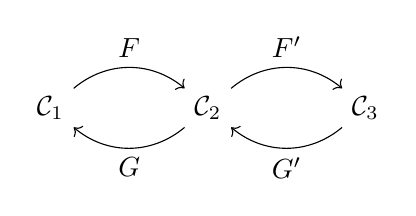
\begin{tikzpicture}
            \node (C1) at (-2,0) {\(\mathcal{C}_1\)};
            \node (C2) at (0,0) {\(\mathcal{C}_2\)};
            \node (C3) at (2,0) {\(\mathcal{C}_3\)};
            \draw[->] (C1) to [bend left = 40] node[above] {\(F\)} (C2);
            \draw[->] (C2) to [bend left = 40] node[above] {\(F^\prime\)} (C3);
            \draw[->] (C2) to [bend left = 40] node[below] {\(G\)} (C1);
            \draw[->] (C3) to [bend left = 40] node[below] {\(G^\prime\)} (C2);
        \end{tikzpicture}
    \end{center}

    \begin{proof}
        给出伴随对应的自然变换 \(\eta, \eta^\prime, \varepsilon, \varepsilon^\prime\),
        定义 \(\xi := (\mathrm{id}_G \ast \eta^\prime \mathrm{id}_{F}) \circ \eta\),
        \(\zeta := \varepsilon^\prime \ast (\varepsilon \ast \mathrm{id}_{G^\prime}) \circ \mathrm{id}_F\),

        \(\xi, \zeta\) 给出 \(F^\prime \circ F \dashv G \circ G^\prime\), 观察以下图表:

        \begin{center}
            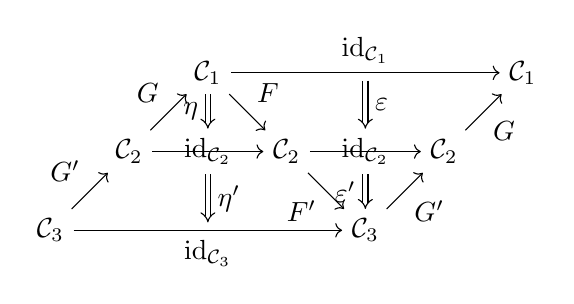
\begin{tikzpicture}
                \node (C11) at (-1,1) {\(\mathcal{C}_1\)};
                \node (C12) at (3,1) {\(\mathcal{C}_1\)};
                \node (C21) at (-2,0) {\(\mathcal{C}_2\)};
                \node (C22) at (0,0) {\(\mathcal{C}_2\)};
                \node (C23) at (2,0) {\(\mathcal{C}_2\)};
                \node (C31) at (-3,-1) {\(\mathcal{C}_3\)};
                \node (C32) at (1,-1) {\(\mathcal{C}_3\)};
                \draw[->] (C11) to node[above] (idc1) {\(\mathrm{id}_{\mathcal{C}_1}\)} (C12);
                \draw[->] (C21) to node (idc21) {\(\mathrm{id}_{\mathcal{C}_2}\)} (C22);
                \draw[->] (C22) to node (idc22) {\(\mathrm{id}_{\mathcal{C}_2}\)} (C23);
                \draw[->] (C31) to node[below] (idc3) {\(\mathrm{id}_{\mathcal{C}_3}\)} (C32);
                \draw[->] (C31) to node[above left] {\(G^\prime\)} (C21);
                \draw[->] (C21) to node[above left] {\(G\)} (C11);
                \draw[->] (C11) to node[above right] {\(F\)} (C22);
                \draw[->] (C22) to node[below left] {\(F^\prime\)} (C32);
                \draw[->] (C32) to node[below right] {\(G^\prime\)} (C23);
                \draw[->] (C23) to node[below right] {\(G\)} (C12);
                \draw[-{Implies},double,double distance = 0.15em] (C11) to node[left] {\(\eta\)} (idc21);
                \draw[-{Implies},double,double distance = 0.15em] (idc21) to node[right] {\(\eta^\prime\)} ($(idc3.north) + (0,0.1)$);
                \draw[-{Implies},double,double distance = 0.15em] (idc22) to node[left] {\(\varepsilon^\prime\)} (C32);
                \draw[-{Implies},double,double distance = 0.15em] ($(idc1.south) + (0,-0.1)$) to node[right] {\(\varepsilon\)} (idc22);
            \end{tikzpicture}
        \end{center}

        此图表合成 \(\mathrm{id}_{G \circ G^\prime}\) 只需注意到上下两个平行四边形均合成单位自然变换, 而左右两个大三角形分别代表 \(\xi, \zeta\),
        另一个图表同理合成 \(\mathrm{id}_{F^\prime \circ F}\).
    \end{proof}
\end{lemma}

\begin{definition}
    我们定义严格的 \(2\) - 范畴为满足如下条件的范畴:

    \begin{enumerate}
        \item 一个范畴 \(\mathcal{C}\).
        \item 任取 \(X,Y \in \mathrm{Ob} (\mathcal{C})\), 有范畴 \(\mathcal{D}\) 使得 \(\mathrm{Mor} (\mathcal{D}) = \mathrm{Hom}_\mathcal{C} (X,Y)\).
        \item 有横合成, 给出 \(f, f^\prime \in \mathrm{Hom}_\mathcal{C} (X,Y)\), \(g, g^\prime \in \mathrm{Hom}_\mathcal{C} (Y,Z)\), 与
                \(2\) - 态射 \(\phi : f \to f^\prime\), \(\psi : g \to g^\prime\), 存在态射 \(\phi \ast \psi : g \circ f \to g^\prime \circ f^\prime\).
        \item 横合成结合, 且与纵合成交换.
        \item 两个单位横合成仍是单位.
    \end{enumerate}
\end{definition}

记原范畴的元素为 \(\mathrm{Mor}_0\), 原范畴的态射为 \(\mathrm{Mor}_1\), 称 \(1\) - 态射, \(2\) - 态射记为 \(\mathrm{Mor}_2\).

\begin{example}
    \(\mathbf{Cat}\) 是严格的 \(2\) - 范畴, 对象是全体小范畴, 态射是范畴间的函子, \(2\) - 态射是自然变换.
\end{example}

我们可以绘制 \(2\) - 范畴对应的图表, 用 \(\Rightarrow\) 表示 \(2\) - 态射, 依旧用 \(\mathrm{Hom}\) 表示两点间态射对应的范畴.

\begin{definition}[Kan 延拓]
    在严格 \(2\) - 范畴 \(\Theta\) 中给出对象 \(\mathcal{C},\mathcal{D},\mathcal{E} \in \mathrm{Mor}_0 (\Theta)\),
    给出 \(1\) - 态射 \(F : \mathcal{C} \to \mathcal{E}, K : \mathcal{C} \to \mathcal{D}\).

    定义左 Kan 延拓 \(\mathrm{Lan}_K F : \mathcal{D} \to \mathcal{E}\) 与其对应的 \(2\) - 态射 \(\eta : F \to \mathrm{Lan}_K F \circ K\),
    满足任给 \(G : \mathcal{D} \to \mathcal{E}\) 与 \(2\) - 态射 \(\phi : F \to G \circ K\), 存在唯一的 \(2\) - 态射 \(\phi^\prime : \mathrm{Lan}_K F \to G\), 满足以下等式:

    \[
        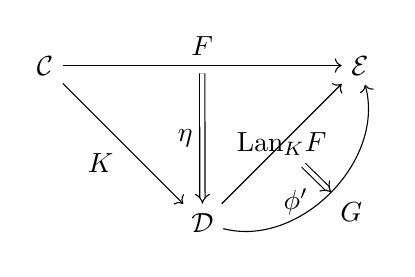
\begin{tikzpicture}
            \node (C) at (-2,2) {\(\mathcal{C}\)};
            \node (D) at (0,0) {\(\mathcal{D}\)};
            \node (E) at (2,2) {\(\mathcal{E}\)};
            \draw[->] (C) to node[above] (F) {\(F\)} (E);
            \draw[->] (C) to node[below left] {\(K\)} (D);
            \draw[->] (D) to [bend right = 60] node[below right] (G) {\(G\)} (E);
            \draw[->] (D) to node (Lan) {\(\mathrm{Lan}_K F\)} (E);
            \draw[-{Implies},double,double distance = 0.15em] ($(F.south) + (0 , - 0.1)$) to node[left] {\(\eta\)} (D);
            \draw[-{Implies},double,double distance = 0.15em] (Lan) to node[below left] {\(\phi^\prime\)} (G);
        \end{tikzpicture} = 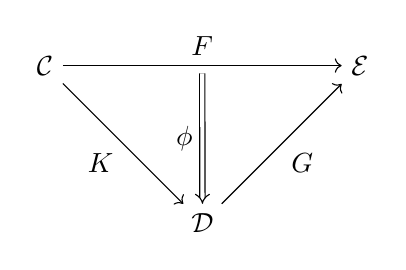
\begin{tikzpicture}
            \node (C) at (-2,2) {\(\mathcal{C}\)};
            \node (D) at (0,0) {\(\mathcal{D}\)};
            \node (E) at (2,2) {\(\mathcal{E}\)};
            \draw[->] (C) to node[above] (F) {\(F\)} (E);
            \draw[->] (C) to node[below left] {\(K\)} (D);
            \draw[->] (D) to node[below right] (G) {\(G\)} (E);
            \draw[-{Implies},double,double distance = 0.15em] ($(F.south) + (0 , - 0.1)$) to node[left] {\(\phi\)} (D);
        \end{tikzpicture}
    \]

    对偶的, 定义右 Kan 延拓 \(\mathrm{Ran}_K F : \mathcal{D} \to \mathcal{E}\) 与其对应的 \(2\) - 态射 \(\varepsilon : \mathrm{Ran}_K F \circ K \to F\),
    满足任给 \(G : \mathcal{D} \to \mathcal{E}\) 与 \(2\) - 态射 \(\phi : G \circ K \to F\), 存在唯一的 \(2\) - 态射 \(\phi^\prime : G \to \mathrm{Ran}_K F\), 满足以下等式:

    \[
        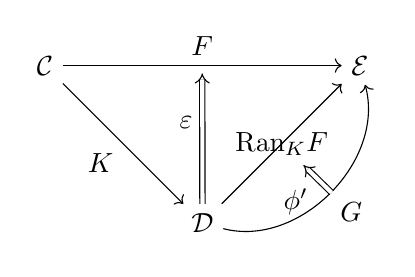
\begin{tikzpicture}
            \node (C) at (-2,2) {\(\mathcal{C}\)};
            \node (D) at (0,0) {\(\mathcal{D}\)};
            \node (E) at (2,2) {\(\mathcal{E}\)};
            \draw[->] (C) to node[above] (F) {\(F\)} (E);
            \draw[->] (C) to node[below left] {\(K\)} (D);
            \draw[->] (D) to [bend right = 60] node[below right] (G) {\(G\)} (E);
            \draw[->] (D) to node (Ran) {\(\mathrm{Ran}_K F\)} (E);
            \draw[-{Implies},double,double distance = 0.15em] (D) to node[above left] {\(\varepsilon\)} ($(F.south) + (0 , - 0.1)$);
            \draw[-{Implies},double,double distance = 0.15em] (G) to node[below left] {\(\phi^\prime\)} (Ran);
        \end{tikzpicture} = 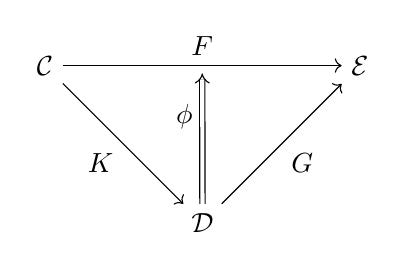
\begin{tikzpicture}
            \node (C) at (-2,2) {\(\mathcal{C}\)};
            \node (D) at (0,0) {\(\mathcal{D}\)};
            \node (E) at (2,2) {\(\mathcal{E}\)};
            \draw[->] (C) to node[above] (F) {\(F\)} (E);
            \draw[->] (C) to node[below left] {\(K\)} (D);
            \draw[->] (D) to node[below right] (G) {\(G\)} (E);
            \draw[-{Implies},double,double distance = 0.15em] (D) to node[above left] {\(\phi\)} ($(F.south) + (0 , - 0.1)$);
        \end{tikzpicture}
    \]
\end{definition}

\begin{lemma}
    Kan 延拓存在则在同构意义下唯一.

    \begin{proof}
        利用泛性质唯一性.
    \end{proof}
\end{lemma}

\begin{lemma}
    如若所有 \(F : \mathcal{C} \to \mathcal{E}\) 的右 Kan 延拓存在, 则 \(\mathrm{Ran}_K\) 给出
    从 \(\mathrm{Hom} (\mathcal{C}, \mathcal{E})\) 到 \(\mathrm{Hom} (\mathcal{D}, \mathcal{E})\) 的函子.

    \begin{proof}
        需给出 \(\mathrm{Ran}_K\) 对态射的作用, 给出 \(F \to G\) 的态射 \(\phi : F \to G\), 定义 \(\mathrm{Ran}_K \phi\) 为使得以下等式成立的唯一态射:

        \[
            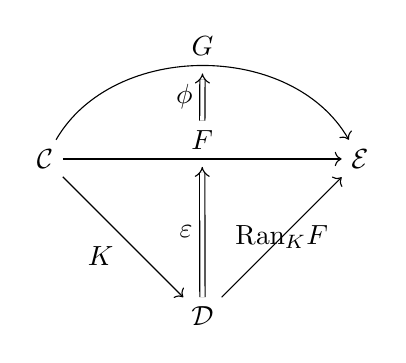
\begin{tikzpicture}
                \node (C) at (-2,2) {\(\mathcal{C}\)};
                \node (D) at (0,0) {\(\mathcal{D}\)};
                \node (E) at (2,2) {\(\mathcal{E}\)};
                \draw[->] (C) to node[above] (F) {\(F\)} (E);
                \draw[->] (C) to [bend left = 60] node[above] (G) {\(G\)} (E);
                \draw[->] (C) to node[below left] {\(K\)} (D);
                \draw[->] (D) to node (Ran) {\(\mathrm{Ran}_K F\)} (E);
                \draw[-{Implies},double,double distance = 0.15em] (D) to node[left] {\(\varepsilon\)} ($(F.south) + (0 , - 0.1)$);
                \draw[-{Implies},double,double distance = 0.15em] (F) to node[left] {\(\phi\)} ($(G.south) + (0 , - 0.1)$);
            \end{tikzpicture} = 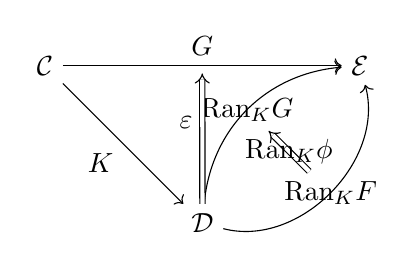
\begin{tikzpicture}
                \node (C) at (-2,2) {\(\mathcal{C}\)};
                \node (D) at (0,0) {\(\mathcal{D}\)};
                \node (E) at (2,2) {\(\mathcal{E}\)};
                \draw[->] (C) to node[above] (G) {\(G\)} (E);
                \draw[->] (C) to node[below left] {\(K\)} (D);
                \draw[->] (D) to [bend left = 40] node (RanG) {\(\mathrm{Ran}_K G\)} (E);
                \draw[->] (D) to [bend right = 60] node (RanF) {\(\mathrm{Ran}_K F\)} (E);
                \draw[-{Implies},double,double distance = 0.15em] (RanF) to node {\(\mathrm{Ran}_K \phi\)} (RanG);
                \draw[-{Implies},double,double distance = 0.15em] (D) to node[above left] {\(\varepsilon\)} ($(G.south) + (0 , - 0.1)$);
            \end{tikzpicture}
        \]

        函子性由唯一性保证.
    \end{proof}
\end{lemma}

\begin{corollary}
    同理, 假定对于所有 \(F : \mathcal{C} \to \mathcal{E}\) 的左 Kan 延拓存在, 则 \(\mathrm{Lan}_K\) 也给出
    从 \(\mathrm{Hom} (\mathcal{C}, \mathcal{E})\) 到 \(\mathrm{Hom} (\mathcal{D}, \mathcal{E})\) 的函子.
\end{corollary}

\begin{lemma}
    有伴随对 \(\mathrm{Lan}_K \dashv (- \circ K) \dashv \mathrm{Ran}_K\), 其中 \((- \circ K)\) 
    定义为将 \(1\) - 态射合成 \(K\), 而将 \(2\) - 态射横合成 \(\mathrm{id}_K\).

    \begin{proof}
        态射集 \(\mathrm{Hom}_{\mathrm{Hom} (\mathcal{D}, \mathcal{E})} (\mathrm{Lan}_K (F),G) \to \mathrm{Hom}_{\mathrm{Hom} (\mathcal{C}, \mathcal{E})} (F,G \circ K)\)
        无非是定义的复写. 在 \(F\) 处自然性是按 \(\mathrm{Lan}_K\) 对态射变换的定义, 在  \(G\) 处的自然性依赖唯一性.
    \end{proof}
\end{lemma}

\begin{lemma}
    在 \(\mathbf{Cat}\) 中考虑, 伴随对 \(F \dashv G\) 给出 Kan 延拓 \(G = \mathrm{Lan}_F (\mathrm{id}_\mathcal{C})\), \(F = \mathrm{Ran}_G (\mathrm{id}_\mathcal{C})\).

    \begin{proof}
        观察下图的合成

        \begin{center}
            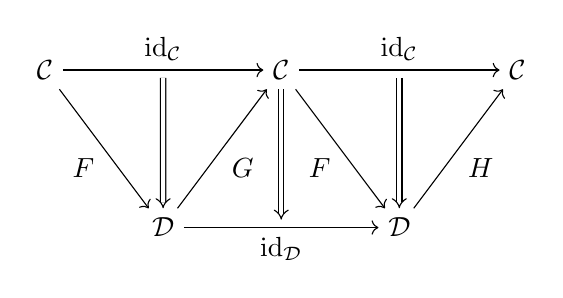
\begin{tikzpicture}
                \node (C1) at (-3,1) {\(\mathcal{C}\)};
                \node (C2) at (0,1) {\(\mathcal{C}\)};
                \node (C3) at (3,1) {\(\mathcal{C}\)};
                \node (D1) at (-1.5,-1) {\(\mathcal{D}\)};
                \node (D2) at (1.5,-1) {\(\mathcal{D}\)};
                \draw[->] (C1) to node[above] (idc1) {\(\mathrm{id}_{\mathcal{C}}\)} (C2);
                \draw[->] (C2) to node[above] (idc2) {\(\mathrm{id}_{\mathcal{C}}\)} (C3);
                \draw[->] (D1) to node[below] (idd) {\(\mathrm{id}_{\mathcal{D}}\)} (D2);
                \draw[->] (C1) to node[below left] {\(F\)} (D1);
                \draw[->] (C2) to node[below left] {\(F\)} (D2);
                \draw[->] (D1) to node[below right] {\(G\)} (C2);
                \draw[->] (D2) to node[below right] {\(H\)} (C3);
                \draw[-{Implies},double,double distance = 0.15em] ($(idc1.south) + (0,-0.1)$) to (D1);
                \draw[-{Implies},double,double distance = 0.15em] (C2) to ($(idd.north) + (0,0.1)$);
                \draw[-{Implies},double,double distance = 0.15em] ($(idc2.south) + (0,-0.1)$) to (D2);
            \end{tikzpicture}
        \end{center}

        所需 \(2\) 态射为右侧平行四边形, 另一个方向亦然.
    \end{proof}
\end{lemma}

\subsection{极限}

定义 \(\mathbf{1}\) 为最简单的范畴, 仅有一个对象与一个态射, 记为 \(\bullet\), 任何
范畴都有唯一的函子 \(\mathbf{1} \to \mathcal{C}\).

\begin{definition}[极限]
    在范畴 \(\mathbf{Cat}\) 中考虑.
    
    给出小范畴 \(I\) 与函子 \(F : I \to \mathcal{C}\), \(K : I \to \mathbf{1}\), 
    若 \(\mathrm{Ran}_K F\) 存在, 则称 \(\mathrm{Ran}_K F\) 为 \(F\) 的极限 (limit), 记为 \(\varprojlim F\),
    对称的 \(\mathrm{Lan}_K F\) 称为 \(F\) 的余极限 (colimit), 记为 \(\varinjlim F\), 称 \(I^\mathrm{op}\) 为极限对应的指标, \(I\) 为余极限对应的指标.
\end{definition}

解释一下上述对于极限的定义, 给出一个 \(\mathbf{1}\) 出发的函子, 即选中了 \(\mathcal{C}\) 中的一个对象 (此对象沿用上述符号记作 \(\varprojlim F\) 或 \(\varinjlim F\)),
极限构造中上述 Kan 延拓给出的自然变换标记了从该对象出发的函子到 \(F I\) 中一对象的态射, 满足对于任意 \(f \in \mathrm{Mor}(I)\), 下图交换:

\begin{center}
    \begin{tikzpicture}
        \node (FX) at (-2,2) {\(F X\)};
        \node (FY) at (2,2) {\(F Y\)};
        \node (lim) at (0,0) {\(\varprojlim F\)};
        \draw[->] (FX) to node[above] (Ff) {\(F f\)} (FY);
        \draw[->] (lim) to (FX);
        \draw[->] (lim) to (FY);
    \end{tikzpicture}
\end{center}

Kan 延拓的性质也就被解为, 对于任意给出的 \(L \in \mathcal{C}\), 一族态射 \(\phi_X : L \to F X\), 使得对于任意 \(f \in \mathrm{Mor}(I)\), 下图交换:

\begin{center}
    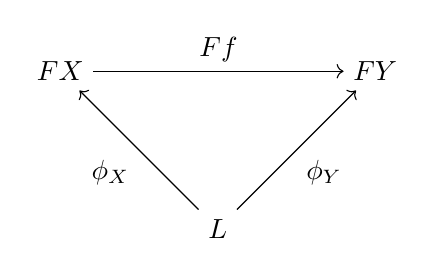
\begin{tikzpicture}
        \node (FX) at (-2,2) {\(F X\)};
        \node (FY) at (2,2) {\(F Y\)};
        \node (L) at (0,0) {\(L\)};
        \draw[->] (FX) to node[above] (Ff) {\(F f\)} (FY);
        \draw[->] (L) to node[below left] (phiX) {\(\phi_X\)} (FX);
        \draw[->] (L) to node[below right] (phiY) {\(\phi_Y\)} (FY);
    \end{tikzpicture}
\end{center}

都有唯一的态射 \(\phi_f : L \to \varprojlim F\), 使得对于任意 \(X \in \mathrm{Ob} (I)\) 下图交换:

\begin{center}
    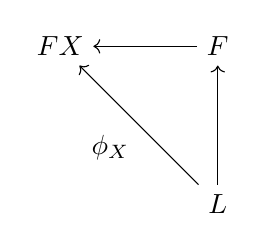
\begin{tikzpicture}
        \node (FX) at (-2,2) {\(F X\)};
        \node (L) at (0,0) {\(L\)};
        \node (lim) at (0,2) {\(\varprojlim F\)};
        \draw[->] (lim) to (FX);
        \draw[->] (L) to node[below left] (phiX) {\(\phi_X\)} (FX);
        \draw[->] (L) to (lim);
    \end{tikzpicture}
\end{center}

余极限将上述所有箭头反向即可得到.

\begin{definition}
    直积 (product) 与余积 (coproduct) 是极限与余极限的特例, 分别对应于 \(I\) 为离散范畴的极限与余极限.
\end{definition}

\begin{example}
    \(\mathbf{Set}\) 中直积为笛卡尔积, 余积为不交并.
\end{example}

\begin{definition}
    等化子 (equalizer) 与余等化子 (coequalizer) 是极限与余极限的特例, 分别对应于 \(I\) 为下图所示的范畴的极限与余极限 (\(\mathrm{id}\) 未画出).

    \begin{center}
        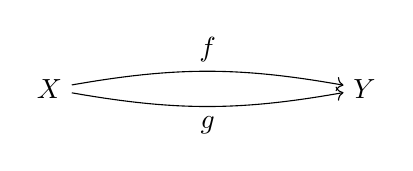
\begin{tikzpicture}
            \node (X) at (-2,0) {\(X\)};
            \node (Y) at (2,0) {\(Y\)};
            \draw[->] (X) to [bend left = 10] node[above] (f) {\(f\)} (Y);
            \draw[->] (X) to [bend right = 10] node[below] (g) {\(g\)} (Y);
        \end{tikzpicture}
    \end{center}
\end{definition}

\begin{lemma}
    \label {lemma:existence of limitation of homeomorphism}
    给出自然变换 \(\psi : \alpha \to \alpha^\prime\), 假使极限存在则存在唯一 \(\psi\) 使对任意 \(i\) 以下图表交换:

    \begin{center}
        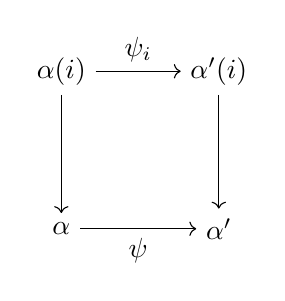
\begin{tikzpicture}
            \node (ai) at (-1,1) {\(\alpha (i)\)};
            \node (api) at (1,1) {\(\alpha^\prime (i)\)};
            \node (lima) at (-1,-1) {\(\varinjlim \alpha\)};
            \node (limap) at (1,-1) {\(\varinjlim \alpha^\prime\)};
            \draw[->] (ai) to node[above] (aii) {\(\psi_i\)} (api);
            \draw[->] (ai) to (lima);
            \draw[->] (api) to (limap);
            \draw[->] (lima) to node[below] (limf) {\(\varinjlim \psi\)} (limap);
        \end{tikzpicture}
    \end{center}

    \begin{proof}
        态射合成给出了 \(\alpha(i) \to \varinjlim \alpha^\prime\), 其与 \(\mathrm{Mor}(I)\) 相容, 由极限的定义唯一性给出了 \(\varinjlim \alpha \to \varinjlim \alpha^\prime\).
    \end{proof}
\end{lemma}

\begin{corollary}
    给出自然变换 \(\psi : \alpha \to \alpha^\prime\), 假使极限存在则存在唯一 \(\psi\) 使对任意 \(i\) 以下图表交换:

    \begin{center}
        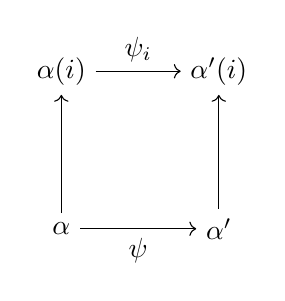
\begin{tikzpicture}
            \node (ai) at (-1,1) {\(\alpha (i)\)};
            \node (api) at (1,1) {\(\alpha^\prime (i)\)};
            \node (lima) at (-1,-1) {\(\varprojlim \alpha\)};
            \node (limap) at (1,-1) {\(\varprojlim \alpha^\prime\)};
            \draw[->] (ai) to node[above] (aii) {\(\psi_i\)} (api);
            \draw[->] (lima) to (ai);
            \draw[->] (limap) to (api);
            \draw[->] (lima) to node[below] (limf) {\(\varprojlim \psi\)} (limap);
        \end{tikzpicture}
    \end{center}
\end{corollary}

\begin{lemma}
    给出自然变换 \(\psi : \alpha_1 \to \alpha_2\),  \(\phi : \alpha_2 \to \alpha_3\), 假使极限存在则有等式 \(\varinjlim (\phi \psi) = \varinjlim \phi \varinjlim \psi\).

    \begin{proof}
            无非是交换图表:

            \begin{center}
                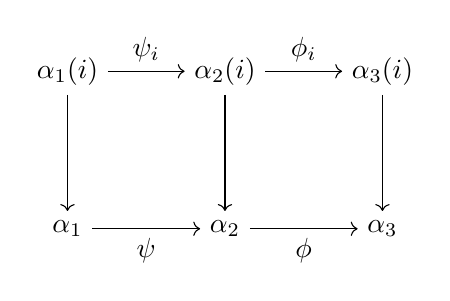
\begin{tikzpicture}
                    \node (a1i) at (-2,1) {\(\alpha_1 (i)\)};
                    \node (a2i) at (0,1) {\(\alpha_2 (i)\)};
                    \node (a3i) at (2,1) {\(\alpha_3 (i)\)};
                    \node (lima1) at (-2,-1) {\(\varinjlim \alpha_1\)};
                    \node (lima2) at (0,-1) {\(\varinjlim \alpha_2\)};
                    \node (lima3) at (2,-1) {\(\varinjlim \alpha_3\)};
                    \draw[->] (a1i) to node[above] (psi) {\(\psi_i\)} (a2i);
                    \draw[->] (a2i) to node[above] (phi) {\(\phi_i\)} (a3i);
                    \draw[->] (a1i) to (lima1);
                    \draw[->] (a2i) to (lima2);
                    \draw[->] (a3i) to (lima3);
                    \draw[->] (lima1) to node[below] (limpsi) {\(\varinjlim \psi\)} (lima2);
                    \draw[->] (lima2) to node[below] (limphi) {\(\varinjlim \phi\)} (lima3);
                \end{tikzpicture}
            \end{center}
    \end{proof}
\end{lemma}

\begin{corollary}
    同理有等式 \(\varprojlim (\phi \psi) = \varprojlim \phi \varprojlim \psi\).
\end{corollary}

\begin{lemma}
    直积的直积 (余积的余积) 为直积 (余积).

    \begin{proof}
        给出对象 \(X_{i,j}\) 的直积 \(X_{i} := \prod_j X_{i,j}\) 与直积 \(X := \prod_i X_i\),
        无非是说对于任意对象 \(Y\), \(\prod_{i,j} \mathrm{Hom} (Y,X_{i,j})\) 与 \(\prod_i \mathrm{Hom} (Y,X_i)\), \(\mathrm{Hom} (Y,X)\) 一一对应,
        老直积态射的合成给出新直积所需的态射.
    \end{proof}
\end{lemma}

\begin{definition}
    考察以下范畴 \(I\):

    \begin{center}
        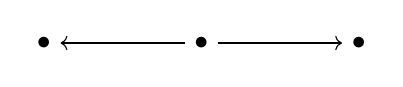
\begin{tikzpicture}
            \node (B1) at (-2,0) {\(\bullet\)};
            \node (B2) at (0,0) {\(\bullet\)};
            \node (B3) at (2,0) {\(\bullet\)};
            \draw[->] (B2) to (B1);
            \draw[->] (B2) to (B3);
        \end{tikzpicture}
    \end{center}

    以 \(I\) 为指标的极限称纤维积 (fibre product) 或拉回 (pullback), \(I\) 的余极限称纤维余积或推出 (pushout), 记作 Cartesius 图表:

    \begin{center}
        \begin{tikzpicture}
            \node (prod) at (-1,1) {\(X \times_Z Y\)};
            \node (X) at (1,1) {\(X\)};
            \node (Y) at (-1,-1) {\(Y\)};
            \node (Z) at (1,-1) {\(Z\)};
            \draw[->] (X) to (Z);
            \draw[->] (Y) to (Z);
            \draw[->] (prod) to (X);
            \draw[->] (prod) to (Y);
            \node at (0,0) {\(\Box\)};
        \end{tikzpicture} \begin{tikzpicture}
            \node (coprod) at (-1,1) {\(X \sqcup_Z Y\)};
            \node (X) at (1,1) {\(X\)};
            \node (Y) at (-1,-1) {\(Y\)};
            \node (Z) at (1,-1) {\(Z\)};
            \draw[->] (Z) to (X);
            \draw[->] (Z) to (Y);
            \draw[->] (X) to (coprod);
            \draw[->] (Y) to (coprod);
            \node at (0,0) {\(\boxplus\)};
        \end{tikzpicture}
    \end{center}
\end{definition}

\begin{definition}
    若范畴 \(\mathcal{C}\) 满足所有以某个小范畴为指标的 \(\varprojlim\) 存在
    则 \(\mathcal{C}\) 是完备的, 对称的 \(\varinjlim\) 存在则 \(\mathcal{C}\) 是余完备的.
\end{definition}

\begin{lemma}
    对于完备的范畴 \(\mathcal{C}\), \(\varinjlim\) 与 \(\varprojlim\) 给出了 \(\mathbf{Fun} (I,\mathcal{C})\) 到 \(\mathcal{C}\) 的函子.
\end{lemma}

\begin{definition}
    定义拟序集 \(P\) 的范畴, 其对象为 \(P\) 中的元素, 在 \(X \leq Y\) 时 \(\abs{\mathrm{Hom} (X,Y)} = 1\) 的范畴.
\end{definition}

\begin{lemma}[Freyd]
    小范畴 \(\mathcal{C}\) 完备当且仅当 \(\mathcal{C}\) 从某个拟序集 \(P\) 构造出来, 且 \(P\) 中每个子集都有下确界.

    \begin{proof}
        假定有 \(f,g : X \to Y\), 则 \(\abs{\mathrm{Hom} (X,Y^{\abs{\mathrm{Mor} (\mathcal{C})}})} > \mathrm{Mor} (\mathcal{C})\)
        矛盾, 此时极限就是下确界.
    \end{proof}
\end{lemma}

\begin{theorem}
    假使范畴 \(\mathcal{C}\) 含所有直积与等化子, 则 \(\mathcal{C}\) 是完备的.

    \begin{proof}
        给出小范畴 \(I\) 与函子 \(F : I \to \mathcal{C}\), 令 \(X := \prod_{i \in \mathrm{Ob} (I)} F i\),
        \(Y := \prod_{\sigma \in \mathrm{Mor} (\mathcal{C})} F (t (\sigma))\), \(Z := \prod_{\sigma \in \mathrm{Mor} (\mathcal{C})} F (s (\sigma))\),
        考察 \(X \to Y\) 的两个态射, 一个逐点, 一个逐点透过 \(Z\), 然后透过 \(\sigma\), 其等化子自然与 \(\sigma\) 相容, 即为极限.
    \end{proof}
\end{theorem}

\begin{corollary}
    假使范畴 \(\mathcal{C}\) 含所有余积与余等化子, 则 \(\mathcal{C}\) 是余完备的.
\end{corollary}

\begin{lemma}
    \(\mathbf{Set}\) 是完备的.

    \begin{proof}
        显然 \(\mathbf{Set}\) 含所有直积, 余积, 等化子, 余等化子.
    \end{proof}
\end{lemma}

\begin{definition}[滤过]
    \setlabel {滤过}
    \label {definition:filtered category}
    给出小范畴 \(I\), 若任取 \(i,j \in \mathrm{Ob} (I)\), 存在 \(k \in \mathrm{Ob} (I)\), 使得 \(i,j\) 到 \(k\) 有态射,
    且对于任意 \(f,g : i \to j\), 存在 \(h : j \to k\), 使得 \(h f = h g\), 则称 \(I\) 滤过 (filtered).
\end{definition}

滤过的好处在于允许我们显式地在某些特定的范畴 (如 \(\mathbf(Set)\)) 中构造余极限, 因为此处等化子是可以直接写出来的等价关系.

\begin{lemma}
    \(\mathcal{C}^{\wedge}\) 与 \(\mathcal{C}^{\vee}\) 是完备且余完备的.

    \begin{proof}
        只需给 \(\mathcal{C}\) 中每一个点赋予极限与余极限, 利用 \ref {lemma:existence of limitation of homeomorphism} 即可.
    \end{proof}
\end{lemma}

这里要注意到嵌入的过程, 假若嵌入 \(\mathbf{Set}^\mathrm{op}\), 而在 \(\mathbf{Set}\) 中考虑对应极限, 需转换 \(\lim\) 方向.

\begin{lemma}
    \label {lemma:existence of limit iff representable}
    函子 \(\alpha : I \to \mathcal{C}\) 余极限存在当且仅当米田嵌入之后的余极限可表, 极限亦然.

    \begin{proof}
        米田嵌入给出的 \(\mathrm{Hom}\) 集的对应无非就是极限的定义.
    \end{proof}
\end{lemma}

\begin{definition}
    极限存在时, 称函子 \(F\) 保 \(\varprojlim \alpha\), 如果 \(F \varprojlim \alpha \simeq \varprojlim F \alpha\), 亦定义保 \(\varinjlim \alpha\).
\end{definition}

\begin{corollary}
    取 \(X \in \mathcal{C}\), 则函子 \(\mathrm{Hom} (X,-)\) 保 \(\varprojlim\), \(\mathrm{Hom} (-,X)\) 保 \(\varinjlim\).
\end{corollary}

\begin{theorem}
    若 \(F \dashv G\), 则 \(F\) 保 \(\varinjlim\), \(G\) 保 \(\varprojlim\).

    \begin{proof}
        考察 \(\mathcal{C}^{\vee}\) 中的等式:

        \[
            \begin{aligned}
                \mathrm{Hom}_{\mathcal{D}} (F \varinjlim \alpha, -) & \simeq \mathrm{Hom}_\mathcal{C} (\varinjlim \alpha, G (-)) \\
                & \simeq \varinjlim \mathrm{Hom}_\mathcal{C} (\alpha (i), G (-)) \\
                & \simeq \varinjlim \mathrm{Hom}_\mathcal{D} (F \alpha (i), -) \\
                & \simeq \mathrm{Hom}_\mathcal{D} (\varinjlim F \alpha, -)
            \end{aligned}
        \]

        依米田嵌入全忠实性, 此给出二者之同构.
    \end{proof}
\end{theorem}

    \section{张量范畴}

本章所论范畴默认是小的, 以免去一些不必要的集合论的困难.

\subsection{幺半范畴}

\subsubsection{定义}

\begin{example}
    我们先来考虑一类最简单的幺半范畴, 对于一个只有一个对象的严格 \(2\) - 范畴,
    定义一个范畴, 其对象为 \(\mathrm{Hom} (\bullet,\bullet)\), 态射为 \(2\) - 态射.

    注意到有择定对象 \(\mathbf{1} = \mathrm{id}\), 并且给出了 \(\mathrm{id} \circ -\) 和 \(- \circ \mathrm{id}\)
    作为范畴的自同构, 对于两个对象, 可以找到对应的 \(f \circ g\), 对于两个态射, 亦给出对应的合成为横合成.
\end{example}

\begin{definition}[幺半范畴]
    \label {definition:monoidal category}

    一个幺半范畴包含资料 \((\mathcal{C},\otimes,a,\mathbf{1},\iota)\), 其中 \(\mathcal{C}\) 是一个范畴,
    \(\otimes\) 是一个 \(\mathcal{C} \times \mathcal{C} \to \mathcal{C}\) 的函子, \(a\) 是两个 \(\mathcal{C} \times \mathcal{C} \times \mathcal{C} \to \mathcal{C}\)
    函子间的自然同构 \((- \otimes -) \otimes - \to - \otimes (- \otimes -)\) 称结合同构, \(\mathbf{1}\) 是 \(\mathcal{C}\) 中对象, 
    而 \(\iota\) 给出态射 \(\mathbf{1} \otimes \mathbf{1} \to \mathbf{1}\).

    满足五边形公理:
    \setlabel {五边形公理}
    \label {axiom:MC pentagon axiom}

    \begin{center}
        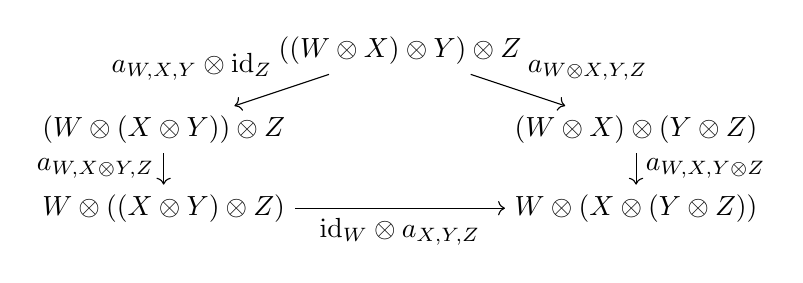
\begin{tikzpicture}
            \node (ararar) at (0,1) {\(((W \otimes X) \otimes Y) \otimes Z\)};
            \node (araarr) at (3,0) {\((W \otimes X) \otimes (Y \otimes Z)\)};
            \node (aarrar) at (-3,0) {\((W \otimes (X \otimes Y)) \otimes Z\)};
            \node (aaarrr) at (3,-1) {\(W \otimes (X \otimes (Y \otimes Z))\)};
            \node (aararr) at (-3,-1) {\(W \otimes ((X \otimes Y) \otimes Z)\)};

            \draw[->] (ararar) to node[above right] {\(a_{W \otimes X,Y,Z}\)} (araarr);
            \draw[->] (ararar) to node[above left] {\(a_{W,X,Y} \otimes \mathrm{id}_Z\)} (aarrar);
            \draw[->] (araarr) to node[right] {\(a_{W,X,Y \otimes Z}\)} (aaarrr);
            \draw[->] (aarrar) to node[left] {\(a_{W,X \otimes Y,Z}\)} (aararr);
            \draw[->] (aararr) to node[below] {\(\mathrm{id}_W \otimes a_{X,Y,Z}\)} (aaarrr);
        \end{tikzpicture}
    \end{center}

    与单位公理, 即以下定义的
    \setlabel {单位公理}
    \label {axiom:MC unit axiom}

        \[
            \begin{aligned}
                L_1 &: X \mapsto \mathbf{1} \otimes X, f \mapsto f \otimes \mathrm{id}_{\mathbf{1}} \\
                R_1 &: X \mapsto X \otimes \mathbf{1}, f \mapsto \mathrm{id}_{\mathbf{1}} \otimes f
            \end{aligned}
        \]

    \(L_1,R_1\) 给出了范畴 \(\mathcal{C} \to \mathcal{C}\) 的等价.
\end{definition}

我们常常用 \(\mathcal{C}\) 代指幺半范畴 \((\mathcal{C},\otimes,a,\mathbf{1},\iota)\).

\begin{definition}[子幺半范畴]
    对一个幺半范畴 \((\mathcal{C}, \otimes,a,\mathbf{1},\iota)\) 其子幺半范畴是指资料 \((\mathcal{D}, \otimes,a,\mathbf{1},\iota)\),
    满足 \(\mathcal{D}\) 是 \(\mathcal{C}\) 的子范畴, 且上述资料构成幺半范畴
\end{definition}

\begin{definition}[对偶幺半范畴]
    对一个幺半范畴 \((\mathcal{C}, \otimes,a,\mathbf{1},\iota)\), 其对偶幺半范畴为资料 \((\mathcal{C}^{\mathrm{op}}, \otimes^\mathrm{op}, a^\mathrm{op},\mathbf{1},\iota)\),
    满足 \(X \otimes^\mathrm{op} Y = Y \otimes X\) 与结合同构的变换 \(a_{X,Y,Z}^{\mathrm{op}} := a_{Z,Y,X}^{-1}\).
\end{definition}

\subsubsection{基本性质}

在幺半范畴中进行讨论, 常常运用添上 \(\mathbf{1}\) 并且使用 \(a,\iota\) 进行消去的技巧.

\begin{definition}
    定义自然同构 \(\lambda,\rho\) 

    \[
        \begin{aligned}
            \lambda_X &: \mathbf{1} \otimes X \to X \\
            \rho_X &: X \otimes \mathbf{1} \to X
        \end{aligned}
    \]

    为以下态射在 \(L_1,R_1\) 下的逆:

    \[
        \begin{aligned}
            \mathbf{1} \otimes (\mathbf{1} \otimes X) &\xrightarrow{a_{\mathbf{1},\mathbf{1},X}^{-1}} (\mathbf{1} \otimes \mathbf{1}) \otimes X \xrightarrow{\iota \otimes \mathrm{id}_X} \mathbf{1} \otimes X \\
            (X \otimes \mathbf{1}) \otimes \mathbf{1} &\xrightarrow{a_{X,\mathbf{1},\mathbf{1}}} X \otimes (\mathbf{1} \otimes \mathbf{1}) \xrightarrow{\mathrm{id}_X \otimes \iota} X \otimes \mathbf{1}
        \end{aligned}
    \]

    或者写成等式:

    \[
        \begin{aligned}
            \mathrm{id}_{\mathbf{1}} \otimes \lambda_X &= (\iota \otimes \mathrm{id}_X) \circ a_{\mathbf{1},\mathbf{1},X}^{-1}\\
            \rho_X \otimes \mathrm{id}_{\mathbf{1}} &= (\mathrm{id}_X \otimes \iota) \circ a_{X,\mathbf{1},\mathbf{1}}
        \end{aligned}
    \]

    自然性源于其为自然变换的复合.
\end{definition}

\begin{lemma}
    自然变换 \(\lambda,\rho\) 满足如下等式:

    \[
        \begin{aligned}
            \lambda_{\mathbf{1} \otimes X} &= \mathrm{id}_{\mathbf{1}} \otimes \lambda_X \\
            \rho_{X \otimes \mathbf{1}} &= \rho_X \otimes \mathrm{id}_{\mathbf{1}}
        \end{aligned}
    \]

    \begin{proof}
        基于 \(\lambda,\rho\) 为自然变换, 给出所有映射皆为同构的交换图表:

        \begin{center}
            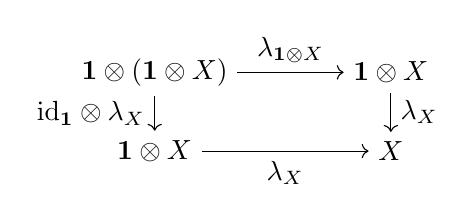
\begin{tikzpicture}
                \node (11x) at (-1.5,0.5) {\(\mathbf{1} \otimes (\mathbf{1} \otimes X)\)};
                \node (1x01) at (1.5,0.5) {\(\mathbf{1} \otimes X\)};
                \node (1x02) at (-1.5,-0.5) {\(\mathbf{1} \otimes X\)};
                \node (x) at (1.5,-0.5) {\(X\)};

                \draw[->] (11x) to node[above] {\(\lambda_{\mathbf{1} \otimes X}\)} (1x01);
                \draw[->] (11x) to node[left] {\(\mathrm{id}_{\mathbf{1}} \otimes \lambda_X\)} (1x02);
                \draw[->] (1x01) to node[right] {\(\lambda_X\)} (x);
                \draw[->] (1x02) to node[below] {\(\lambda_X\)} (x);
            \end{tikzpicture} 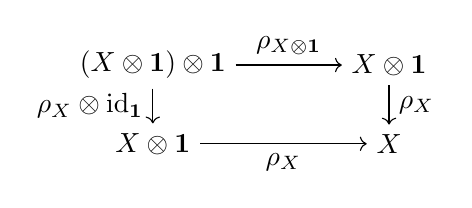
\begin{tikzpicture}
                \node (x11) at (-1.5,0.5) {\((X \otimes \mathbf{1}) \otimes \mathbf{1}\)};
                \node (x101) at (1.5,0.5) {\(X \otimes \mathbf{1}\)};
                \node (x102) at (-1.5,-0.5) {\(X \otimes \mathbf{1}\)};
                \node (x) at (1.5,-0.5) {\(X\)};

                \draw[->] (x11) to node[above] {\(\rho_{X \otimes \mathbf{1}}\)} (x101);
                \draw[->] (x11) to node[left] {\(\rho_X \otimes \mathrm{id}_{\mathbf{1}}\)} (x102);
                \draw[->] (x101) to node[right] {\(\rho_X\)} (x);
                \draw[->] (x102) to node[below] {\(\rho_X\)} (x);
            \end{tikzpicture}
        \end{center}
    \end{proof}
\end{lemma}

\begin{lemma}
    有交换图表:

    \begin{center}
        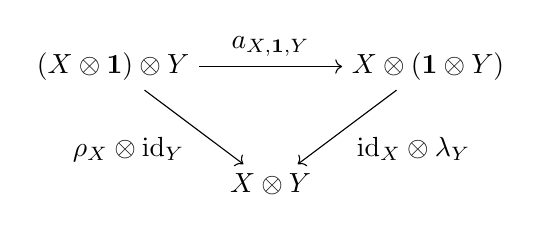
\begin{tikzpicture}
            \node (x1yl) at (-2,0.5) {\((X \otimes \mathbf{1}) \otimes Y\)};
            \node (x1yr) at (2,0.5) {\(X \otimes (\mathbf{1} \otimes Y)\)};
            \node (xy) at (0,-1) {\(X \otimes Y\)};

            \draw[->] (x1yl) to node[above] {\(a_{X,\mathbf{1},Y}\)} (x1yr);
            \draw[->] (x1yl) to node[below left] {\(\rho_X \otimes \mathrm{id}_Y\)} (xy);
            \draw[->] (x1yr) to node[below right] {\(\mathrm{id}_X \otimes \lambda_Y\)} (xy);
        \end{tikzpicture}
    \end{center}

    \begin{proof}
        注意到以下所有映射均为同构的交换图表, 其余小图形和外框交换, 故中心小三角形交换.

        \begin{center}
            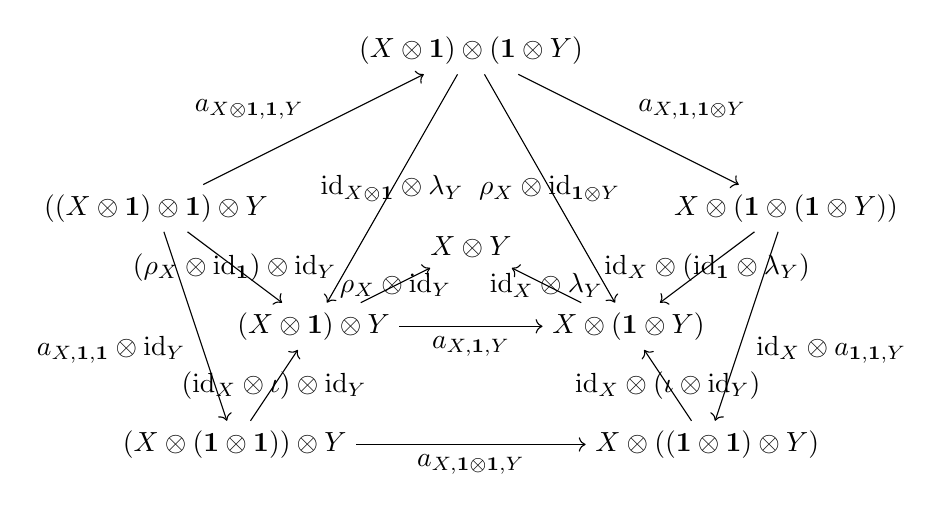
\begin{tikzpicture}
                \node (lx1rl1yr) at (0,3) {\((X \otimes \mathbf{1}) \otimes (\mathbf{1} \otimes Y)\)};
                \node (llx1r1ry) at (-4,1) {\(((X \otimes \mathbf{1}) \otimes \mathbf{1}) \otimes Y\)};
                \node (xl1l1yrr) at (4,1) {\(X \otimes (\mathbf{1} \otimes (\mathbf{1} \otimes Y))\)};
                \node (lxl11rry) at (-3,-2) {\((X \otimes (\mathbf{1} \otimes \mathbf{1})) \otimes Y\)};
                \node (xll11ryr) at (3,-2) {\(X \otimes ((\mathbf{1} \otimes \mathbf{1}) \otimes Y)\)};
                \node (lx1ry) at (-2,-0.5) {\((X \otimes \mathbf{1}) \otimes Y\)};
                \node (xl1yr) at (2,-0.5) {\(X \otimes (\mathbf{1} \otimes Y)\)};
                \node (xy) at (0,0.5) {\(X \otimes Y\)};

                \draw[->] (lx1rl1yr) to node[above right] {\(a_{X,\mathbf{1},\mathbf{1} \otimes Y}\)} (xl1l1yrr);
                \draw[->] (llx1r1ry) to node[above left] {\(a_{X \otimes \mathbf{1},\mathbf{1},Y}\)} (lx1rl1yr);
                \draw[->] (llx1r1ry) to node[below left] {\(a_{X,\mathbf{1},\mathbf{1}} \otimes \mathrm{id}_Y\)} (lxl11rry);
                \draw[->] (xl1l1yrr) to node[below right] {\(\mathrm{id}_X \otimes a_{\mathbf{1},\mathbf{1},Y}\)} (xll11ryr);
                \draw[->] (lxl11rry) to node[below] {\(a_{X,\mathbf{1} \otimes \mathbf{1},Y}\)} (xll11ryr);
                \draw[->] (lx1rl1yr) to node {\(\mathrm{id}_{X \otimes \mathbf{1}} \otimes \lambda_Y\)} (lx1ry);
                \draw[->] (lx1rl1yr) to node {\(\rho_X \otimes \mathrm{id}_{\mathbf{1} \otimes Y}\)} (xl1yr);
                \draw[->] (xl1l1yrr) to node {\(\mathrm{id}_X \otimes (\mathrm{id}_\mathbf{1} \otimes \lambda_Y)\)} (xl1yr);
                \draw[->] (xll11ryr) to node {\(\mathrm{id}_X \otimes (\iota \otimes \mathrm{id}_Y)\)} (xl1yr);
                \draw[->] (llx1r1ry) to node {\((\rho_X \otimes \mathrm{id}_\mathbf{1}) \otimes \mathrm{id}_Y\)} (lx1ry);
                \draw[->] (lxl11rry) to node {\((\mathrm{id}_X \otimes \iota) \otimes \mathrm{id}_Y\)} (lx1ry);
                \draw[->] (lx1ry) to node[below] {\(a_{X,\mathbf{1},Y}\)} (xl1yr);
                \draw[->] (lx1ry) to node {\(\rho_X \otimes \mathrm{id}_Y\)} (xy);
                \draw[->] (xl1yr) to node {\(\mathrm{id}_X \otimes \lambda_Y\)} (xy);
            \end{tikzpicture}
        \end{center}
    \end{proof}
\end{lemma}

\begin{corollary}
    上图中取 \(X = Y = \mathbf{1}\) 有:

    \[
        \lambda_{\mathbf{1}} = \rho_{\mathbf{1}} = \iota
    \]
\end{corollary}

\begin{lemma}
    有交换图表:

    \begin{center}
        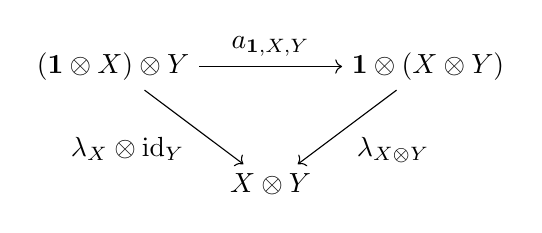
\begin{tikzpicture}
            \node (l1xry) at (-2,0.5) {\((\mathbf{1} \otimes X) \otimes Y\)};
            \node (1lxyr) at (2,0.5) {\(\mathbf{1} \otimes (X \otimes Y)\)};
            \node (xy) at (0,-1) {\(X \otimes Y\)};

            \draw[->] (l1xry) to node[above] {\(a_{\mathbf{1},X,Y}\)} (1lxyr);
            \draw[->] (l1xry) to node[below left] {\(\lambda_X \otimes \mathrm{id}_Y\)} (xy);
            \draw[->] (1lxyr) to node[below right] {\(\lambda_{X \otimes Y}\)} (xy);
        \end{tikzpicture}

        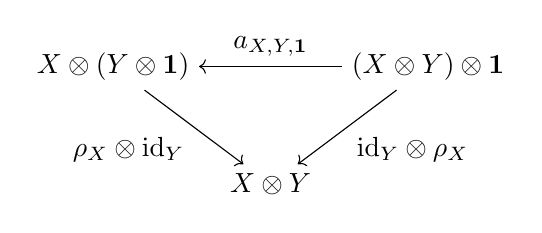
\begin{tikzpicture}
            \node (xly1r) at (-2,0.5) {\(X \otimes (Y \otimes \mathbf{1})\)};
            \node (lxyr1) at (2,0.5) {\((X \otimes Y) \otimes \mathbf{1}\)};
            \node (xy) at (0,-1) {\(X \otimes Y\)};

            \draw[->] (lxyr1) to node[above] {\(a_{X,Y,\mathbf{1}}\)} (xly1r);
            \draw[->] (lxyr1) to node[below right] {\(\mathrm{id}_Y \otimes \rho_X\)} (xy);
            \draw[->] (xly1r) to node[below left] {\(\rho_X \otimes \mathrm{id}_Y\)} (xy);
        \end{tikzpicture}
    \end{center}

    \begin{proof}
        同理观察全部态射均为同构的以下交换图表, 外框与其余小图形交换, 故左上角小三角形交换, 依赖 \(\mathbf{1} \otimes -\) 给出等价,
        第二幅图亦可对称的在对偶范畴中选取, 依赖 \(- \otimes \mathbf{1}\) 给出等价.

        \begin{center}
            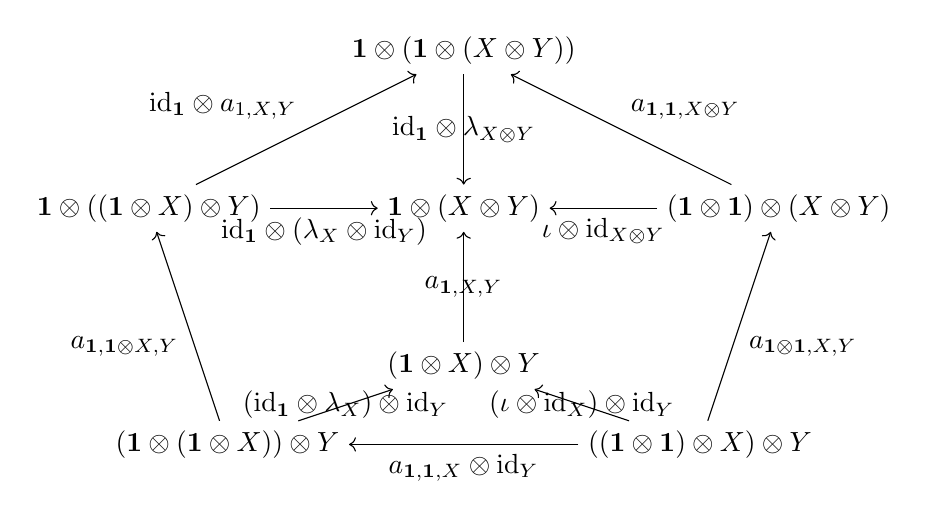
\begin{tikzpicture}
                \node (1ll1xryr) at (-4,1) {\(\mathbf{1} \otimes ((\mathbf{1} \otimes X) \otimes Y)\)};
                \node (l1l1xrry) at (-3,-2) {\((\mathbf{1} \otimes (\mathbf{1} \otimes X)) \otimes Y\)};
                \node (1l1lxyrr) at (0,3) {\(\mathbf{1} \otimes (\mathbf{1} \otimes (X \otimes Y))\)};
                \node (ll11rxry) at (3,-2) {\(((\mathbf{1} \otimes \mathbf{1}) \otimes X) \otimes Y\)};
                \node (l11rlxyr) at (4,1) {\((\mathbf{1} \otimes \mathbf{1}) \otimes (X \otimes Y)\)};
                \node (l1xry) at (0,-1) {\((\mathbf{1} \otimes X) \otimes Y\)};
                \node (1lxyr) at (0,1) {\(\mathbf{1} \otimes (X \otimes Y)\)};

                \draw[->] (1ll1xryr) to node[above left] {\(\mathrm{id}_\mathbf{1} \otimes a_{1,X,Y}\)} (1l1lxyrr);
                \draw[->] (l1l1xrry) to node[below left] {\(a_{\mathbf{1},\mathbf{1} \otimes X,Y}\)} (1ll1xryr);
                \draw[->] (ll11rxry) to node[below] {\(a_{\mathbf{1},\mathbf{1},X} \otimes \mathrm{id}_Y\)} (l1l1xrry);
                \draw[->] (l11rlxyr) to node[above right] {\(a_{\mathbf{1},\mathbf{1},X \otimes Y}\)} (1l1lxyrr);
                \draw[->] (ll11rxry) to node[below right] {\(a_{\mathbf{1} \otimes \mathbf{1},X,Y}\)} (l11rlxyr);
                \draw[->] (1ll1xryr) to node[below] {\(\mathrm{id}_\mathbf{1} \otimes (\lambda_{X} \otimes \mathrm{id}_Y)\)} (1lxyr);
                \draw[->] (l1l1xrry) to node {\((\mathrm{id}_\mathbf{1} \otimes \lambda_X) \otimes \mathrm{id}_Y\)} (l1xry);
                \draw[->] (1l1lxyrr) to node {\(\mathrm{id}_\mathbf{1} \otimes \lambda_{X \otimes Y}\)} (1lxyr);
                \draw[->] (ll11rxry) to node {\((\iota \otimes \mathrm{id}_X) \otimes \mathrm{id}_Y\)} (l1xry);
                \draw[->] (l11rlxyr) to node[below] {\(\iota \otimes \mathrm{id}_{X \otimes Y}\)} (1lxyr);
                \draw[->] (l1xry) to node {\(a_{\mathbf{1},X,Y}\)} (1lxyr);
            \end{tikzpicture}
        \end{center}
    \end{proof}
\end{lemma}

\begin{axiom}
    \setlabel {三角形公理}
    \label {axiom:MC triangle axiom}
    上述三个三角形交换图表称为三角形公理.
\end{axiom}

\begin{definition}[幺半范畴]
    一个幺半范畴包含资料 \((\mathcal{C},\otimes,a,\mathbf{1},\lambda,\rho)\), 其中 \(\mathcal{C}\) 是一个范畴,
    \(\otimes\) 是一个 \(\mathcal{C} \times \mathcal{C} \to \mathcal{C}\) 的函子, \(a\) 是两个 \(\mathcal{C} \times \mathcal{C} \times \mathcal{C} \to \mathcal{C}\) 函子间的自然同构,
    \(\mathbf{1}\) 是 \(\mathcal{C}\) 中对象, \(\lambda,\rho\) 是 \(\mathbf{1} \otimes -, - \otimes \mathbf{1} \to -\) 的自然同构, 满足 \ref{axiom:MC pentagon axiom}, \ref{axiom:MC triangle axiom}.

    \begin{proof}
        只需验证 \(\lambda_\mathbf{1} = \rho_\mathbf{1} = \iota\), 以及此给出的 \(\iota\) 诱导出同样的 \(\lambda,\rho\).

        反过来, 有下述图表交换, 于是最下方梯形交换, 从而 \(\lambda_\mathbf{1} = \rho_\mathbf{1} = \iota\), 
        \(\iota\) 给出 \(\lambda,\rho\) 是三角形公理取 \(X = \mathbf{1}\) 或 \(Y = \mathbf{1}\) 给出的.

        \begin{center}
            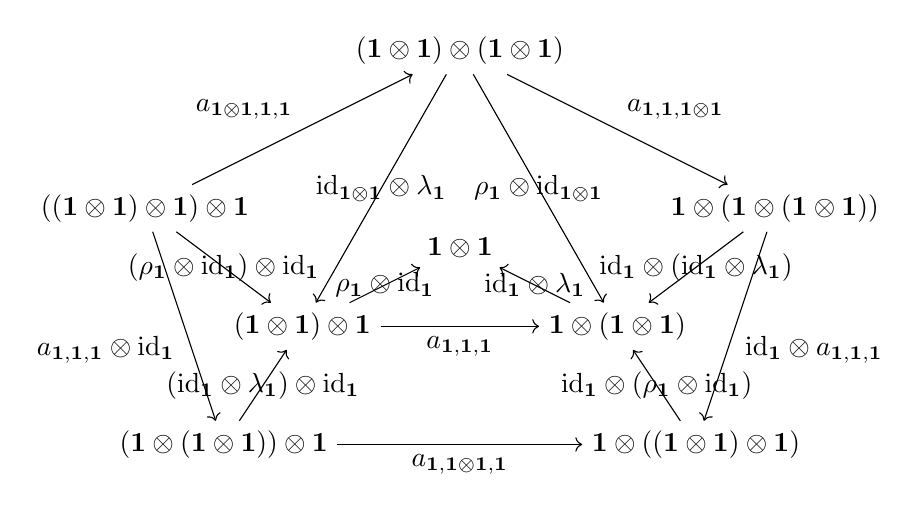
\begin{tikzpicture}
                \node (lx1rl1yr) at (0,3) {\((\mathbf{1} \otimes \mathbf{1}) \otimes (\mathbf{1} \otimes \mathbf{1})\)};
                \node (llx1r1ry) at (-4,1) {\(((\mathbf{1} \otimes \mathbf{1}) \otimes \mathbf{1}) \otimes \mathbf{1}\)};
                \node (xl1l1yrr) at (4,1) {\(\mathbf{1} \otimes (\mathbf{1} \otimes (\mathbf{1} \otimes \mathbf{1}))\)};
                \node (lxl11rry) at (-3,-2) {\((\mathbf{1} \otimes (\mathbf{1} \otimes \mathbf{1})) \otimes \mathbf{1}\)};
                \node (xll11ryr) at (3,-2) {\(\mathbf{1} \otimes ((\mathbf{1} \otimes \mathbf{1}) \otimes \mathbf{1})\)};
                \node (lx1ry) at (-2,-0.5) {\((\mathbf{1} \otimes \mathbf{1}) \otimes \mathbf{1}\)};
                \node (xl1yr) at (2,-0.5) {\(\mathbf{1} \otimes (\mathbf{1} \otimes \mathbf{1})\)};
                \node (xy) at (0,0.5) {\(\mathbf{1} \otimes \mathbf{1}\)};

                \draw[->] (lx1rl1yr) to node[above right] {\(a_{\mathbf{1},\mathbf{1},\mathbf{1} \otimes \mathbf{1}}\)} (xl1l1yrr);
                \draw[->] (llx1r1ry) to node[above left] {\(a_{\mathbf{1} \otimes \mathbf{1},\mathbf{1},\mathbf{1}}\)} (lx1rl1yr);
                \draw[->] (llx1r1ry) to node[below left] {\(a_{\mathbf{1},\mathbf{1},\mathbf{1}} \otimes \mathrm{id}_\mathbf{1}\)} (lxl11rry);
                \draw[->] (xl1l1yrr) to node[below right] {\(\mathrm{id}_\mathbf{1} \otimes a_{\mathbf{1},\mathbf{1},\mathbf{1}}\)} (xll11ryr);
                \draw[->] (lxl11rry) to node[below] {\(a_{\mathbf{1},\mathbf{1} \otimes \mathbf{1},\mathbf{1}}\)} (xll11ryr);
                \draw[->] (lx1rl1yr) to node {\(\mathrm{id}_{\mathbf{1} \otimes \mathbf{1}} \otimes \lambda_\mathbf{1}\)} (lx1ry);
                \draw[->] (lx1rl1yr) to node {\(\rho_\mathbf{1} \otimes \mathrm{id}_{\mathbf{1} \otimes \mathbf{1}}\)} (xl1yr);
                \draw[->] (xl1l1yrr) to node {\(\mathrm{id}_\mathbf{1} \otimes (\mathrm{id}_\mathbf{1} \otimes \lambda_\mathbf{1})\)} (xl1yr);
                \draw[->] (xll11ryr) to node {\(\mathrm{id}_\mathbf{1} \otimes (\rho_\mathbf{1} \otimes \mathrm{id}_\mathbf{1})\)} (xl1yr);
                \draw[->] (llx1r1ry) to node {\((\rho_\mathbf{1} \otimes \mathrm{id}_\mathbf{1}) \otimes \mathrm{id}_\mathbf{1}\)} (lx1ry);
                \draw[->] (lxl11rry) to node {\((\mathrm{id}_\mathbf{1} \otimes \lambda_\mathbf{1}) \otimes \mathrm{id}_\mathbf{1}\)} (lx1ry);
                \draw[->] (lx1ry) to node[below] {\(a_{\mathbf{1},\mathbf{1},\mathbf{1}}\)} (xl1yr);
                \draw[->] (lx1ry) to node {\(\rho_\mathbf{1} \otimes \mathrm{id}_\mathbf{1}\)} (xy);
                \draw[->] (xl1yr) to node {\(\mathrm{id}_\mathbf{1} \otimes \lambda_\mathbf{1}\)} (xy);
            \end{tikzpicture}
        \end{center}
    \end{proof}
\end{definition}

\subsubsection{幺半函子}

\begin{definition}[幺半函子]
    两个幺半范畴 \(\mathfrak{C} := (\mathcal{C},\otimes,a,\mathbf{1},\iota), \mathfrak{C}^\prime := (\mathcal{C}^\prime,\otimes^\prime,a^\prime,\mathbf{1}^\prime,\iota^\prime)\),
    一个幺半函子 \(\mathfrak{F} : \mathfrak{C} \to \mathfrak{C}^\prime\) 是一个函子 \(F : \mathcal{C} \to \mathcal{C}^\prime\), 与一个 \(\mathcal{C} \times \mathcal{C} \to \mathcal{C}^\prime\)
    上的自然同构 \(J :(F(-) \otimes^\prime F(-)) \to F ((-) \otimes (-))\), 与同构 \(F (\mathbf{1}) \to \mathbf{1}^\prime\), 以及以下交换图表:

    \begin{center}
        \begin{tikzpicture}
            \node (lfxfyrfz) at (-3,1.5) {\((F(X) \otimes^\prime F(Y)) \otimes^\prime F(Z)\)};
            \node (fxlfyfzr) at (3,1.5) {\(F(X) \otimes^\prime (F(Y) \otimes^\prime F(Z))\)};
            \node (fxyfz) at (-3,0) {\(F(X \otimes Y) \otimes^\prime F(Z)\)};
            \node (fxfyz) at (3,0) {\(F(X) \otimes^\prime F(Y \otimes Z)\)};
            \node (flxyrz) at (-3,-1.5) {\(F((X \otimes Y) \otimes Z)\)};
            \node (lfxlyzr) at (3,-1.5) {\(F(X \otimes (Y \otimes Z))\)};

            \draw[->] (lfxfyrfz) to node[above] {\(a^\prime_{F(X),F(Y),F(Z)}\)} (fxlfyfzr);
            \draw[->] (lfxfyrfz) to node[left] {\(J_{X,Y} \otimes^\prime \mathrm{id}_{F(Z)}\)} (fxyfz);
            \draw[->] (fxlfyfzr) to node[right] {\(\mathrm{id}_{F(X)} \otimes^\prime J_{Y,Z}\)} (fxfyz);
            \draw[->] (fxyfz) to node[left] {\(J_{X \otimes Y,Z}\)} (flxyrz);
            \draw[->] (fxfyz) to node[right] {\(J_{X,Y \otimes Z}\)} (lfxlyzr);
            \draw[->] (flxyrz) to node[below] {\(F(a_{X,Y,Z})\)} (lfxlyzr);
        \end{tikzpicture}
    \end{center}

    \setlabel {幺半结构公理}
    \label {axiom:MC monoidal functor axiom}
    以上图表称为幺半结构公理.
\end{definition}

\begin{definition}[幺半等价]
    一个幺半函子 \(\mathfrak{F} : \mathfrak{C} \to \mathfrak{C}^\prime\) 是一个幺半等价, 若 \(F\) 是 \(\mathcal{C} \to \mathcal{C}^\prime\) 的等价.
\end{definition}

\begin{lemma}
    \label {lemma:MC canonical isomorphism}
    同构 \(\phi : \mathbf{1}^\prime \to F(\mathbf{1})\) 有典范的选取, 使得以下所有映射皆为同构的交换图表成立:
    \begin{center}
        \begin{tikzpicture}
            \node (1fx) at (-2,0.5) {\(\mathbf{1}^\prime \otimes^\prime F(X)\)};
            \node (fx) at (2,0.5) {\(F(X)\)};
            \node (f1fx) at (-2,-0.5) {\(F(\mathbf{1}) \otimes^\prime F(X)\)};
            \node (f1x) at (2,-0.5) {\(F(\mathbf{1} \otimes X)\)};

            \draw[->] (1fx) to node[above] {\(\lambda^\prime_{F(X)}\)} (fx);
            \draw[->] (1fx) to node[left] {\(\phi \otimes^\prime \mathrm{id}_{F(X)}\)} (f1fx);
            \draw[->] (f1x) to node[right] {\(F(\lambda_X)\)} (fx);
            \draw[->] (f1fx) to node[below] {\(J_{\mathbf{1},X}\)} (f1x);
        \end{tikzpicture}
    \end{center}

    \begin{center}
        \begin{tikzpicture}
            \node (flxr1) at (-2,0.5) {\(F(X) \otimes^\prime \mathbf{1}^\prime\)};
            \node (fx) at (2,0.5) {\(F(X)\)};
            \node (fxf1) at (-2,-0.5) {\(F(X) \otimes^\prime F(\mathbf{1})\)};
            \node (flx1r) at (2,-0.5) {\(F(X \otimes \mathbf{1})\)};

            \draw[->] (flxr1) to node[above] {\(\rho^\prime_{F(X)}\)} (fx);
            \draw[->] (flxr1) to node[left] {\(\mathrm{id}_{F(X)} \otimes^\prime \phi\)} (fxf1);
            \draw[->] (flx1r) to node[right] {\(F(\rho_X)\)} (fx);
            \draw[->] (fxf1) to node[below] {\(J_{X,\mathbf{1}}\)} (flx1r);
        \end{tikzpicture}
    \end{center}

    \begin{proof}
        在第一幅图中取 \(X = \mathbf{1}\), 构造出对应的 \(\phi\), 函子 \(- \otimes^\prime F(\mathbf{1})\) 典范同构于函子 \(- \otimes^\prime \mathbf{1}^\prime\), 故其存在,
        需证明以上图表对于任意 \(X\) 成立.

        验证以下交换图表, 其余小图形与外框交换故左上大三角交换, 而依赖于 \(- \otimes^\prime F(\mathbf{1})\) 给出范畴等价知其给出第二幅图片, 在第二幅图中取 \(X = \mathbf{1}\)
        反过来可对称的验证第一幅图.

        \begin{center}
            \begin{tikzpicture}
                \node (lfxf1rf1) at (-3.8,3) {\((F(X) \otimes^\prime F(\mathbf{1})) \otimes^\prime F(\mathbf{1})\)};
                \node (fxlf1f1r) at (3.8,3) {\(F(X) \otimes^\prime (F(\mathbf{1}) \otimes^\prime F(\mathbf{1}))\)};
                \node (lfx1rf1) at (-2,1.5) {\((F(X) \otimes^\prime \mathbf{1}^\prime) \otimes^\prime F(\mathbf{1})\)};
                \node (fxl1f1r) at (2,1.5) {\(F(X) \otimes^\prime (\mathbf{1}^\prime \otimes^\prime F(\mathbf{1}))\)};
                \node (fx1f1) at (-3.8,0) {\(F(X \otimes \mathbf{1}) \otimes^\prime F(\mathbf{1})\)};
                \node (fxf1) at (0,0) {\(F(X) \otimes^\prime F(\mathbf{1})\)};
                \node (fxf11) at (3.8,0) {\(F(X) \otimes^\prime F(\mathbf{1} \otimes \mathbf{1})\)};
                \node (fx1) at (0,-1.5) {\(F(X \otimes \mathbf{1})\)};
                \node (flx1r1) at (-3.8,-3) {\(F((X \otimes \mathbf{1}) \otimes \mathbf{1})\)};
                \node (fxl11r) at (3.8,-3) {\(F(X \otimes (\mathbf{1} \otimes \mathbf{1}))\)};

                \draw[->] (lfxf1rf1) to node[above] {\textcolor{blue}{\(a^\prime_{F(X),F(\mathbf{1}),F(\mathbf{1})}\)}} (fxlf1f1r);
                \draw[->] (lfx1rf1) to node {\textcolor{red}{\((\mathrm{id}_{F(X)} \otimes^\prime \phi) \otimes^\prime \mathrm{id}_{F(\mathbf{1})}\)}} (lfxf1rf1);
                \draw[->] (lfxf1rf1) to node[left] {\textcolor{blue}{\(J_{X,\mathbf{1}} \otimes^\prime \mathrm{id}_{F(\mathbf{1})}\)}} (fx1f1);
                \draw[->] (fxlf1f1r) to node[right] {\textcolor{blue}{\(\mathrm{id}_{F(X)} \otimes^\prime J_{\mathbf{1},\mathbf{1}}\)}} (fxf11);
                \draw[->] (lfx1rf1) to node[above] {\textcolor{red}{\(a^\prime_{F(X),\mathbf{1}^\prime,F(\mathbf{1})}\)}} (fxl1f1r);
                \draw[->] (fxl1f1r) to node {\textcolor{red}{\(\mathrm{id}_{F(X)} \otimes^\prime (\phi \otimes^\prime \mathrm{id}_{F(\mathbf{1})})\)}} (fxlf1f1r);
                \draw[->] (lfx1rf1) to node[left] {\textcolor{red}{\(\rho_{F(X)} \otimes^\prime \mathrm{id}_{F(\mathbf{1})}\)}} (fxf1);
                \draw[->] (fxl1f1r) to node[right] {\textcolor{red}{\(\mathrm{id}_{F(X)} \otimes^\prime \lambda^\prime_{F(\mathbf{1})}\)}} (fxf1);
                \draw[->] (fxf1) to node {\(J_{X,\mathbf{1}}\)} (fx1);
                \draw[->] (fx1f1) to node[below] {\textcolor{red}{\(F(\rho_X) \otimes^\prime \mathrm{id}_{F(\mathbf{1})}\)}} (fxf1);
                \draw[->] (fxf11) to node[below] {\textcolor{red}{\(\mathrm{id}_{F(X)} \otimes^\prime F(\lambda_\mathbf{1})\)}} (fxf1);
                \draw[->] (fx1f1) to node[left] {\textcolor{blue}{\(J_{X \otimes \mathbf{1},\mathbf{1}}\)}} (flx1r1);
                \draw[->] (fxf11) to node[right] {\textcolor{blue}{\(J_{X,\mathbf{1} \otimes \mathbf{1}}\)}} (fxl11r);
                \draw[->] (flx1r1) to node[below] {\textcolor{blue}{\(F(a_{X,\mathbf{1},\mathbf{1}})\)}} (fxl11r);
                \draw[->] (flx1r1) to node {\(F(\rho_X \otimes \mathrm{id}_\mathbf{1})\)} (fx1);
                \draw[->] (fxl11r) to node {\(F(\mathrm{id}_X \otimes \lambda_\mathbf{1})\)} (fx1);
            \end{tikzpicture}
        \end{center}
    \end{proof}
\end{lemma}

\begin{definition}[幺半函子]
    一个幺半函子是资料 \((F,J,\phi)\), 其中 \(F : \mathcal{C} \to \mathcal{C}^\prime\) 是一个函子, 
    \(J\) 是一个 \(\mathcal{C} \times \mathcal{C} \to \mathcal{C}^\prime\) 上的自然同构,
    \(\phi : \mathbf{1}^\prime \to F(\mathbf{1})\) 是一个同构, 满足 \ref{axiom:MC monoidal functor axiom} 与 \ref{lemma:MC canonical isomorphism} 中的图表.
\end{definition}

\begin{corollary}
    幺半函子的复合是幺半函子.

    \begin{proof}
        \(J^G\) 自然性可以给出交换图表, 将其嵌入定义与 \ref{axiom:MC monoidal functor axiom} 中的图表, 便得到复合幺半函子的幺半结构公理.

        \begin{center}
            \begin{tikzpicture}
                \node (gfxfygfz) at (-3,0.5) {\((G(F(X) \otimes F(Y))) \otimes G(F(Z))\)};
                \node (gfxfyfz) at (3,0.5) {\(G((F(X) \otimes F(Y)) \otimes F(Z))\)};
                \node (gfxygfz) at (-3,-0.5) {\(G(F(X \otimes Y)) \otimes G(F(Z))\)};
                \node (gfxyfz) at (3,-0.5) {\(G(F(X \otimes Y) \otimes F(Z))\)};

                \draw[->] (gfxfygfz) to node[above] {\(J^G_{F(X) \otimes F(Y),F(Z)}\)} (gfxfyfz);
                \draw[->] (gfxfygfz) to node[left] {\(G(J^F_{X,Y}) \otimes \mathrm{id}_{G(F(Z))}\)} (gfxygfz);
                \draw[->] (gfxfyfz) to node[right] {\(G(J^F_{X,Y} \otimes \mathrm{id}_{F(Z)})\)} (gfxyfz);
                \draw[->] (gfxygfz) to node[below] {\(J^G_{F(X \otimes Y),F(Z)}\)} (gfxyfz);
            \end{tikzpicture}
        \end{center}
    \end{proof}
\end{corollary}

\begin{definition}
    两个幺半函子 \(F_1,F_2 : \mathfrak{C} \to \mathfrak{D}\) 的幺半自然变换命为一个自然变换 \(\alpha : F_1 \to F_2\), 使得以下交换图表成立:

    \begin{center}
        \begin{tikzpicture}
            \node (f1xf1y) at (-2,0.5) {\(F_1(X) \otimes F_1(Y)\)};
            \node (f2xf2y) at (2,0.5) {\(F_2(X) \otimes F_2(Y)\)};
            \node (f1xy) at (-2,-0.5) {\(F_1(X \otimes Y)\)};
            \node (f2xy) at (2,-0.5) {\(F_2(X \otimes Y)\)};

            \draw[->] (f1xf1y) to node[above] {\(\alpha_X \otimes \alpha_Y\)} (f2xf2y);
            \draw[->] (f1xf1y) to node[left] {\(J_{1,X,Y}\)} (f1xy);
            \draw[->] (f2xf2y) to node[right] {\(J_{2,X,Y}\)} (f2xy);
            \draw[->] (f1xy) to node[below] {\(\alpha_{X \otimes Y}\)} (f2xy);
        \end{tikzpicture}
    \end{center}
\end{definition}

\begin{corollary}
    幺半自然变换有横纵合成.

    \begin{proof}
        先验证纵合成, 以下交换图表成立:

        \begin{center}
            \begin{tikzpicture}
                \node (f1xf1y) at (-4,0.5) {\(F_1(X) \otimes F_1(Y)\)};
                \node (f2xf2y) at (0,0.5) {\(F_2(X) \otimes F_2(Y)\)};
                \node (f3xf3y) at (4,0.5) {\(F_3(X) \otimes F_3(Y)\)};
                \node (f1xy) at (-4,-0.5) {\(F_1(X \otimes Y)\)};
                \node (f2xy) at (0,-0.5) {\(F_2(X \otimes Y)\)};
                \node (f3xy) at (4,-0.5) {\(F_3(X \otimes Y)\)};

                \draw[->] (f1xf1y) to node[above] {\(\alpha_X \otimes \alpha_Y\)} (f2xf2y);
                \draw[->] (f2xf2y) to node[above] {\(\beta_X \otimes \beta_Y\)} (f3xf3y);
                \draw[->] (f1xf1y) to node[left] {\(J_{1,X,Y}\)} (f1xy);
                \draw[->] (f2xf2y) to node {\(J_{2,X,Y}\)} (f2xy);
                \draw[->] (f3xf3y) to node[right] {\(J_{3,X,Y}\)} (f3xy);
                \draw[->] (f1xy) to node[below] {\(\alpha_{X \otimes Y}\)} (f2xy);
                \draw[->] (f2xy) to node[below] {\(\beta_{X \otimes Y}\)} (f3xy);
            \end{tikzpicture}
        \end{center}

        再验证横合成, 验证以下交换图表成立:

        \begin{center}
            \begin{tikzpicture}
                \node (11x11y) at (-4,1) {\(F_1 G_1(X) \otimes F_1 G_1(Y)\)};
                \node (12x12y) at (-4,0) {\(F_1 G_2(X) \otimes F_1 G_2(Y)\)};
                \node (22x22y) at (-4,-1) {\(F_2 G_2(X) \otimes F_2 G_2(Y)\)};
                \node (11x1y) at (0,1) {\(F_1 (G_1(X) \otimes G_1(Y))\)};
                \node (12x2y) at (0,0) {\(F_1 (G_2(X) \otimes G_2(Y))\)};
                \node (22x2y) at (0,-1) {\(F_2 (G_2(X) \otimes G_2(Y))\)};
                \node (11xy) at (4,1) {\(F_1 G_1(X \otimes Y)\)};
                \node (12xy) at (4,0) {\(F_1 G_2(X \otimes Y)\)};
                \node (22xy) at (4,-1) {\(F_2 G_2(X \otimes Y)\)};

                \draw[->] (11x11y) to (11x1y);
                \draw[->] (12x12y) to (12x2y);
                \draw[->] (22x22y) to (22x2y);
                \draw[->] (11x11y) to (12x12y);
                \draw[->] (12x12y) to (22x22y);
                \draw[->] (11x1y) to (12x2y);
                \draw[->] (12x2y) to (22x2y);
                \draw[->] (11x1y) to (11xy);
                \draw[->] (12x2y) to (12xy);
                \draw[->] (22x2y) to (22xy);
                \draw[->] (11xy) to (12xy);
                \draw[->] (12xy) to (22xy);
            \end{tikzpicture}
        \end{center}
    \end{proof}
\end{corollary}

\begin{corollary}
    幺半自然变换的复合和自然变换享有一样的运算公式, 即横纵合成结合律与交换律.
\end{corollary}

\begin{corollary}
    幺半范畴的等价是一对幺半函子 \(F,G\) 使得其复合同构于幺半幺半范畴的恒等变换.

    \begin{proof}
        需验证其逆给出确为幺半函子, 假使有幺半函子 \(F : \mathfrak{C} \to \mathfrak{D}\), 有函子 \(G : \mathfrak{D} \to \mathfrak{C}\), 
        以及自然同构 \(\alpha : F \circ G \to \mathrm{id}_\mathfrak{D}\), \(\beta : G \circ F \to \mathrm{id}_\mathfrak{C}\),
        有 \(GX \otimes GY \xrightarrow{\beta_{X \otimes Y}^{-1}} GF (GX \otimes GY) \xrightarrow{GJ_{GX,GY}} G(FGX \otimes FGY) \xrightarrow{G(\alpha_X \otimes \alpha_Y)} GX \otimes GY\),
        可以验证上述态射使 \(G\) 成为幺半函子, 亦考察 \(\alpha,\beta\) 知复合的同构.
    \end{proof}
\end{corollary}

\subsubsection{融贯定理}

我们需说明上述 \ref{axiom:MC pentagon axiom}, \ref{axiom:MC triangle axiom}, 蕴含
所有结合与消去的交换图表都成立.

\begin{lemma}
    给出 \(n + 1\) 个有顺序的对象, 张量积时一共有 \(\frac{1}{n+1} \frac{2n!}{n!n!}\) 种打括号的方式.

    \begin{proof}
        等同于有 \(n + 1\) 个叶节点时满二叉树的数量, 记为计数函数 \(f : \mathbb{Z}_{>0} \to \mathbb{N}\),
        有 \(f(1) = 1, f(k) = \sum_{i=1}^{k-1} f(i) f(k-i)\), 递推得到 \(f(n+1) = \frac{1}{n+1} \frac{2n!}{n!n!}\).
    \end{proof}
\end{lemma}

\begin{theorem}[结合律]
    给出运算 \(R\) 满足 \(X R (Y R Z) = (X R Y) R Z\), 则括号总是可以省略.

    \begin{proof}
        我们先归纳的定义无括号时一种典范的运算顺序如下:

        \[
            X_1 R X_2 R \cdots R X_n = (X_1 R X_2) R \cdots R X_n
        \]

        归纳, 当只有三个对象时, 即为结合律本身, 假定含有 \(n\) 个对象时结合律成立, 则含有 \(n+1\) 个对象时,
        找到最外侧的 \(R\), 将该 \(R\) 右端的对象变成典范的选取, 又 \(A R (B R X_{n+1}) = (A R B) R X_{n+1}\),
        对前 \(n\) 个对象应用归纳假设, 于是得到结合律成立.
    \end{proof}
\end{theorem}

\begin{theorem}[Mac Lane 融贯定理]
    任意给出 \(n\) 个有顺序的对象与对应的张量积, 结合映射复合的结果是唯一的.

    \begin{proof}
        只需证明对于典范选取 \(X_1 \otimes X_2 \otimes \cdots \otimes X_n\) 复合到自身的结合约束是唯一的,
        对 \(n\) 进行归纳, 当 \(n = 4\) 时, 即为五边形公理, 假定 \(n = k\) 时成立, 则 \(n = k+1\) 时, 
        依赖结合律知可以典范的选取结合同态使得 \(X_{k+1}\) 在最外部.

        \[
            A \otimes B \to A \otimes (C \otimes X_{k+1}) \to (A \otimes C) \otimes X_{k+1}
        \]

        依赖于 \(B\) 包含少于 \(k + 1\) 个对象, 应用归纳假设, 上述结合约束是唯一的, 对一个最简的结合态射
        \(S \to S^\prime\), 可分类为四类情况, 第一类为 \(A \otimes B \to A^\prime \otimes B\), 第二类为
        \(A \otimes B \to A \otimes B^\prime\), 第三类为 \(A \otimes (B \otimes C) \to (A \otimes B) \otimes C\),
        第四类为 \((A \otimes B) \otimes C \to A \otimes (B \otimes C)\), 我们需证明典范的将 \(X_{k+1}\) 移动到最外部的结合态射交换.

        第一类可以展开如仪:

        \begin{center}
            \begin{tikzpicture}
                \node (ab) at (-3.5,0.5) {\(A \otimes B\)};
                \node (acx) at (0,0.5) {\(A \otimes (C \otimes X_{k+1})\)};
                \node (apb) at (-3.5,-0.5) {\(A^\prime \otimes B\)};
                \node (apcx) at (0,-0.5) {\(A^\prime \otimes (C \otimes X_{k+1})\)};
                \node (ac) at (3.5,0.5) {\((A \otimes C) \otimes X_{k+1}\)};
                \node (apc) at (3.5,-0.5) {\((A^\prime \otimes C) \otimes X_{k+1}\)};

                \draw[->] (ab) to (acx);
                \draw[->] (ab) to (apb);
                \draw[->] (acx) to (ac);
                \draw[->] (apb) to (apcx);
                \draw[->] (acx) to (apcx);
                \draw[->] (ac) to (apc);
                \draw[->] (apcx) to (apc);
            \end{tikzpicture}
        \end{center}

        第二类无非是归纳假设, 第三类与第四类可以展开如仪, 右侧四边形即 \ref{axiom:MC pentagon axiom}.

        \begin{center}
            \begin{tikzpicture}
                \node (albcr) at (-4,0.5) {\(A \otimes (B \otimes C)\)};
                \node (labrc) at (-4,-0.5) {\((A \otimes B) \otimes C\)};
                \node (albdxr) at (0,0.5) {\(A \otimes (B \otimes (D \otimes X_{k+1}))\)};
                \node (labrdx) at (0,-0.5) {\((A \otimes B) \otimes (D \otimes X_{k+1})\)};
                \node (albdrx) at (4,0.5) {\((A \otimes (B \otimes D)) \otimes X_{k+1}\)};
                \node (labdrx) at (4,-0.5) {\(((A \otimes B) \otimes D) \otimes X_{k+1}\)};

                \draw[->] (albcr) to (albdxr);
                \draw[->] (albcr) to (labrc);
                \draw[->] (albdxr) to (albdrx);
                \draw[->] (labrc) to (labrdx);
                \draw[->] (albdxr) to (labrdx);
                \draw[->] (albdrx) to (labdrx);
                \draw[->] (labrdx) to (labdrx);
            \end{tikzpicture}
        \end{center}

        于是我们对任意的结合态射的复合, 都给出了以下交换图表:

        \begin{center}
            \begin{tikzpicture}
                \node (Sm) at (0,0.5) {\(S_m\)};
                \node (Sm-1) at (-3,0.5) {\(S_{m-1}\)};
                \node (Sm+1) at (3,0.5) {\(S_{m+1}\)};
                \node (Tm) at (0,-0.5) {\(T_m \otimes X_{k+1}\)};
                \node (Tm-1) at (-3,-0.5) {\(T_{m-1} \otimes X_{k+1}\)};
                \node (Tm+1) at (3,-0.5) {\(T_{m+1} \otimes X_{k+1}\)};

                \draw[->] (Sm) to (Tm);
                \draw[->] (Sm-1) to (Sm);
                \draw[->] (Sm) to (Sm+1);
                \draw[->] (Sm+1) to (Tm+1);
                \draw[->] (Tm-1) to (Tm);
                \draw[->] (Tm) to (Tm+1);
                \draw[->] (Sm-1) to (Tm-1);
            \end{tikzpicture}
        \end{center}

        依赖归纳假设, \(T_m\) 给出的结合态射是唯一的, 于是 \(S_m\) 也给出唯一的结合态射.
    \end{proof}
\end{theorem}

\begin{corollary}
    应用 \ref{axiom:MC triangle axiom}, 对 \(\mathbf{1}\) 的消去总是唯一的.
\end{corollary}

\begin{definition}[严格幺半范畴]
    一个严格幺半范畴是一个幺半范畴, 如果满足以下等式:
    \[
        \begin{aligned}
            (X \otimes Y) \otimes Z &= X \otimes (Y \otimes Z) \\
            \mathbf{1} \otimes X &= X \otimes \mathbf{1} = X
        \end{aligned}
    \]
\end{definition}

\begin{theorem}[Mac Lane 严格性定理]
    任意幺半范畴等价于一个严格幺半范畴.

    \begin{proof}
        我们构造出这样一个严格幺半范畴, 使得其在运算过程中隐含类似于上述的迁移过程.

        定义幺半范畴 \(\mathcal{V}\), 其对象为 \((F,\rho)\), 其中 \(F\) 是函子 \(\mathcal{C} \to \mathcal{C}\), 
        \(\rho\) 是自然同态 \(F(-) \otimes - \to F(- \otimes -)\), 使得以下交换图表总是成立:

        \begin{center}
            \begin{tikzpicture}
                \node (ararar) at (0,1) {\((FX \otimes Y) \otimes Z\)};
                \node (araarr) at (3,0) {\(FX \otimes (Y \otimes Z)\)};
                \node (aarrar) at (-3,0) {\(F (X \otimes Y) \otimes Z\)};
                \node (aaarrr) at (3,-1) {\(F (X \otimes (Y \otimes Z))\)};
                \node (aararr) at (-3,-1) {\(F ((X \otimes Y) \otimes Z)\)};
    
                \draw[->] (ararar) to node[above right] {\(a_{FX,Y,Z}\)} (araarr);
                \draw[->] (ararar) to node[above left] {\(\rho_{X,Y} \otimes \mathrm{id}_Z\)} (aarrar);
                \draw[->] (araarr) to node[right] {\(\rho_{X,Y \otimes Z}\)} (aaarrr);
                \draw[->] (aarrar) to node[left] {\(\rho_{X \otimes Y,Z}\)} (aararr);
                \draw[->] (aararr) to node[below] {\(F (a_{X,Y,Z})\)} (aaarrr);
            \end{tikzpicture}
        \end{center}

        其态射是与 \(\rho\) 相容的自然变换 \(\theta : F^1 \to F^2\), 使得以下交换图表成立:

        \begin{center}
            \begin{tikzpicture}
                \node (f1x) at (-2,0.5) {\(F^1(X) \otimes Y\)};
                \node (f2x) at (2,0.5) {\(F^2(X) \otimes Y\)};
                \node (f1xy) at (-2,-0.5) {\(F^1(X \otimes Y)\)};
                \node (f2xy) at (2,-0.5) {\(F^2(X \otimes Y)\)};

                \draw[->] (f1x) to node[above] {\(\theta_X \otimes \mathrm{id}_Y\)} (f2x);
                \draw[->] (f1x) to node[left] {\(\rho_{X,Y}\)} (f1xy);
                \draw[->] (f2x) to node[right] {\(\rho_{X,Y}\)} (f2xy);
                \draw[->] (f1xy) to node[below] {\(\theta_{X \otimes Y}\)} (f2xy);
            \end{tikzpicture}
        \end{center}

        给出幺元 \((\mathrm{id}_{\mathcal{C}},\mathrm{id}_{- \otimes -})\), 定义张量积为 
        \((F^1,\rho^1) \otimes (F^2,\rho^2) := (F^1 \circ F^2, (\mathrm{id}_{F^1} \ast \rho^2) \circ (\rho^1 \ast \mathrm{id}_{F^2 \times \mathrm{id}_\mathcal{C}}))\),
        显见张量积是 \(\mathcal{V} \times \mathcal{V} \to \mathcal{V}\) 的函子.

        于是有自然的嵌入 \(\psi : \mathcal{C} \to \mathcal{V}\), 使得 \(X \mapsto (X \otimes -,a_{X,-,-})\),
        态射 \(f \mapsto f \otimes \mathrm{id}_{-}\), 其与 \(\rho\) 相容源于 \(a\) 自然性.

        所定义的幺半范畴 \(\mathcal{V}\) 是严格幺半范畴, 其有唯一的三元张量积
        \((F^1,\rho^1) \otimes ((F^2,\rho^2) \otimes (F^3,\rho^3)) = (F^1 \circ F^2 \circ F^3, (\mathrm{id}_{F^1} \ast \mathrm{id}_{F^2} \ast \rho^3) \circ (\mathrm{id}_{F^1} \ast \rho^2 \ast \mathrm{id}_{F^3 \times \mathrm{id}_\mathcal{C}}) \circ (\rho^1 \ast \mathrm{id}_{(F^2 \circ F^3) \times \mathrm{id}_{\mathcal{C}}}))\)
        而对单位的消去是显见的.

        乃需验证 \(\psi\) 是幺半等价, 其函子性基于 \(a\) 自然性显然, 定义 
        \(J_{X,Y} := a_{X,Y,-} : \psi(X) \otimes \psi(Y) = (X \otimes (Y \otimes -), (\mathrm{id}_X \otimes a_{Y,-,-}) \circ a_{X,Y \otimes -,-}) \to \psi(X \otimes Y) = ((X \otimes Y) \otimes -,a_{X \otimes Y,-,-})\)
        其与 \(\rho\) 相容无非是 \ref{axiom:MC pentagon axiom}, 而 \(J\) 自然性显然. 其次, 我们考察以下图表给出的 \(F(X) \to G(X)\).

        \begin{center}
            \begin{tikzpicture}
                \node (f1x) at (-3,1) {\(F(\mathbf{1}) \otimes X\)};
                \node (g1x) at (-3,-1) {\(G(\mathbf{1}) \otimes X\)};
                \node (f1xp) at (0,1) {\(F(\mathbf{1} \otimes X)\)};
                \node (g1xp) at (0,-1) {\(G(\mathbf{1} \otimes X)\)};
                \node (fx) at (3,1) {\(F(X)\)};
                \node (gx) at (3,-1) {\(G(X)\)};

                \draw[->] (fx) to node[above] {\(F \lambda_X^{-1}\)} (f1xp);
                \draw[->] (f1xp) to node[above] {\(\rho_{\mathbf{1},X}^{-1}\)} (f1x);
                \draw[->] (g1x) to node[below] {\(\pi_{\mathbf{1},X}\)} (g1xp);
                \draw[->] (g1xp) to node[below] {\(G \lambda_X\)} (gx);
                \draw[->] (f1x) to node[left] {\(f \otimes \mathrm{id}_X\)} (g1x);
                \draw[dashed,->] (f1xp) to (g1xp);
                \draw[dashed,->] (fx) to (gx);
            \end{tikzpicture}
        \end{center}

        从而 \(\mathrm{Hom}_{\mathcal{V}} ((F,\rho),(G,\pi))\) 同构于 \(\mathrm{Hom}_{\mathcal{C}} (F(\mathbf{1}),G(\mathbf{1}))\),
        该同构具自然性, 故 \(\psi\) 是等价.
    \end{proof}
\end{theorem}

上述嵌入亦称幺半米田.

\subsubsection{伴随对象}

\begin{definition}[伴随对象]
    给出幺半范畴 \(\mathcal{C}\), 某个对象 \(X\) 的左伴随是一个对象 \(X^\ast\) 若有两个态射 \(\mathrm{ev}_X : X^\ast \otimes X \to \mathbf{1}, \mathrm{coev}_X : \mathbf{1} \to X \otimes X^\ast\),
    满足等式:

    \[
        \begin{aligned}
            (\mathrm{id}_X \otimes \mathrm{ev}_X) \circ a_{X,X^\ast,X} \circ (\mathrm{coev}_X \otimes \mathrm{id}_X) &= \rho_X^{-1} \circ \lambda_X \\
            (\mathrm{ev}_X \otimes \mathrm{id}_{X^\ast}) \circ a_{X^\ast,X,X^\ast}^{-1} \circ (\mathrm{id}_{X^\ast} \otimes \mathrm{coev}_X) &= \lambda_X^{-1} \circ \rho_X 
        \end{aligned}
    \]

    右伴随是一个对象 \(^\ast X\) 若有两个态射 \(\mathrm{ev}^\prime_X : X \otimes {^\ast X} \to \mathbf{1}, \mathrm{coev}^\prime_X : \mathbf{1} \to {^\ast X} \otimes X\), 满足等式:

    \[
        \begin{aligned}
            (\mathrm{ev}^\prime_X \otimes \mathrm{id}_X) \circ a_{X,{^\ast X},X}^{-1} \circ (\mathrm{id}_X \otimes \mathrm{coev}^\prime_{X}) &= \lambda_X^{-1} \circ \rho_X \\
            (\mathrm{id}_{^\ast X} \otimes X) \circ a_{{^\ast X},X,{^\ast X}} \circ (\mathrm{coev}^\prime_X \otimes \mathrm{id}_{^\ast X}) &= \rho_X^{-1} \circ \lambda_X 
        \end{aligned}
    \]
\end{definition}

\begin{corollary}
    \({^\ast} (X^\ast) \cong X \cong {({^\ast} X)}^\ast\).
\end{corollary}

\begin{corollary}
    \(\mathbf{1}^\ast \cong {^\ast \mathbf{1}} \cong \mathbf{1}\).
\end{corollary}

\begin{corollary}
    左伴随存在则在同构意义下唯一.

    \begin{proof}
        若给出两个左伴随 \(X_1^\ast,X_2^\ast\), 略去所需的结合与消去, 有以下交换图表:

        \begin{center}
            \begin{tikzpicture}
                \node (x11) at (-4,1.5) {\(X_1^\ast\)};
                \node (x2) at (-4,-1.5) {\(X_2^\ast\)};
                \node (x12) at (4,-1.5) {\(X_1^\ast\)};
                \node (x1xx2) at (-4,0) {\(X_1^\ast \otimes X \otimes X_2^\ast\)};
                \node (x1xx2xx1) at (0,0) {\(X_1^\ast \otimes X \otimes X_2^\ast \otimes X \otimes X_1^\ast\)};
                \node (x2xx1) at (0,-1.5) {\(X_2^\ast \otimes X \otimes X_1^\ast\)};
                \node (x1xx11) at (0,1.5) {\(X_1^\ast \otimes X \otimes X_1^\ast\)};
                \node (x1xx12) at (4,0) {\(X_1^\ast \otimes X \otimes X_1^\ast\)};

                \draw[->] (x11) to node[above] {\(\mathrm{id}_{X_1^\ast} \otimes \mathrm{coev}_1\)} (x1xx11);
                \draw[->] (x11) to node[left] {\(\mathrm{id}_{X_1^\ast} \otimes \mathrm{coev}_2\)} (x1xx2);
                \draw[->] (x1xx11) to node {\textcolor{red}{\(\mathrm{id}_{X_1^\ast} \otimes \mathrm{coev}_2 \otimes \mathrm{id}_X \otimes \mathrm{id}_{X_1^\ast}\)}} (x1xx2xx1);
                \draw[->] (x1xx2) to node[above] {\textcolor{red}{\(\mathrm{id}_{X_1^\ast} \otimes \mathrm{id}_X \otimes \mathrm{id}_{X_2^\ast} \otimes \mathrm{coev}_1\)}} (x1xx2xx1);
                \draw[->] (x1xx2) to node[left] {\(\mathrm{ev}_1 \otimes \mathrm{id}_{X_2^\ast}\)} (x2);
                \draw[->] (x1xx2xx1) to node[above] {\textcolor{red}{\(\mathrm{id}_{X_1^\ast} \otimes \mathrm{id}_X \otimes \mathrm{ev}_2 \otimes \mathrm{id}_{X_1^\ast}\)}} (x1xx12);
                \draw[->] (x1xx2xx1) to node {\textcolor{red}{\(\mathrm{ev}_1 \otimes \mathrm{id}_{X_2^\ast} \otimes \mathrm{id}_X \otimes \mathrm{id}_{X_1^\ast}\)}} (x2xx1);
                \draw[->] (x1xx12) to node[right] {\(\mathrm{ev}_1 \otimes \mathrm{id}_{X_1^\ast}\)} (x12);
                \draw[->] (x2) to node[below] {\(\mathrm{id}_{X_2^\ast} \otimes \mathrm{coev}_1\)} (x2xx1);
                \draw[->] (x2xx1) to node[below] {\(\mathrm{ev}_2 \otimes \mathrm{id}_{X_1^\ast}\)} (x12);
                \draw[->] (x1xx11) to (4,1.5) to (x1xx12);
            \end{tikzpicture}
        \end{center}

        同理给出对称的图表, 左上至右下合成 \(\mathrm{id}_{X_2^\ast}\), \(\mathrm{id}_{X_2^\ast}\), 于是 \((\mathrm{ev}_1 \otimes \mathrm{id}_{X_2^\ast}) \circ a_{X_1^\ast,X,X_2^\ast}^{-1} \circ (\mathrm{id}_{X_1^\ast} \otimes \mathrm{coev}_2)\) 和
        \((\mathrm{ev}_2 \otimes \mathrm{id}_{X_1^\ast}) \circ a_{X_2^\ast,X,X_1^\ast}^{-1} \circ (\mathrm{id}_{X_2^\ast} \otimes \mathrm{coev}_1)\) 给出同构.
    \end{proof}
\end{corollary}

\begin{corollary}
    右伴随存在则在同构意义下唯一.

    \begin{proof}
        证明是对称的.
    \end{proof}
\end{corollary}

\begin{definition}
    假设所论的伴随存在, 则 \(f : X \to Y\) 诱导出态射 \(f^\ast : Y^\ast \to X^\ast\) 如下:

    \begin{center}
        \begin{tikzpicture}
            \node (ys) at (-5.5,0.5) {\(Y^\ast\)};
            \node (ysxxs) at (-2,0.5) {\(Y^\ast \otimes (X \otimes X^\ast)\)};
            \node (ysxxsp) at (2,0.5) {\((Y^\ast \otimes X) \otimes X^\ast\)};
            \node (ysyxsp) at (-2,-0.5) {\(Y^\ast \otimes (Y \otimes X^\ast)\)};
            \node (ysyxs) at (2,-0.5) {\((Y^\ast \otimes Y) \otimes X^\ast\)};
            \node (xs) at (5.5,-0.5) {\(X^\ast\)};

            \draw[->] (ys) to node[above] {\(\mathrm{id}_{Y^\ast} \otimes \mathrm{coev}_X\)} (ysxxs);
            \draw[->] (ysxxs) to node[above] {\(a_{Y^\ast,X,X^\ast}^{-1}\)} (ysxxsp);
            \draw[->] (ysyxsp) to node[below] {\(a_{Y^\ast,Y,X^\ast}^{-1}\)} (ysyxs);
            \draw[->] (ysxxs) to node[left] {\(\mathrm{id}_{Y^\ast} \otimes (f \otimes \mathrm{id}_{X^\ast})\)} (ysyxsp);
            \draw[->] (ysxxsp) to node[right] {\((\mathrm{id}_{Y^\ast} \otimes f) \otimes \mathrm{id}_{X^\ast}\)} (ysyxs);
            \draw[->] (ysyxs) to node[below] {\(\mathrm{ev}_Y \otimes \mathrm{id}_{X^\ast}\)} (xs);
        \end{tikzpicture}
    \end{center}

    亦可定义 \(^\ast f : {^\ast Y} \to {^\ast X}\) 如下:

    \begin{center}
        \begin{tikzpicture}
            \node (ys) at (-5.5,0.5) {\(^\ast Y\)};
            \node (xsxys) at (-2,0.5) {\(({^\ast X} \otimes X) \otimes {^\ast Y}\)};
            \node (xsxysp) at (2,0.5) {\({^\ast X} \otimes (X \otimes {^\ast Y})\)};
            \node (xsyysp) at (-2,-0.5) {\(({^\ast X} \otimes Y) \otimes {^\ast Y}\)};
            \node (xsyys) at (2,-0.5) {\({^\ast X} \otimes (Y \otimes {^\ast Y})\)};
            \node (xs) at (5.5,-0.5) {\(^\ast X\)};

            \draw[->] (ys) to node[above] {\(\mathrm{coev}^\prime_X \otimes \mathrm{id}_{^\ast Y}\)} (xsxys);
            \draw[->] (xsxys) to node[above] {\(a_{^\ast X,X,{^\ast Y}}\)} (xsxysp);
            \draw[->] (xsyysp) to node[below] {\(a_{^\ast X,Y,{^\ast Y}}\)} (xsyys);
            \draw[->] (xsxys) to node[left] {\((\mathrm{id}_{^\ast X} \otimes f) \otimes \mathrm{id}_{^\ast Y}\)} (xsyysp);
            \draw[->] (xsxysp) to node[right] {\(\mathrm{id}_{^\ast X} \otimes (f \otimes \mathrm{id}_{^\ast Y})\)} (xsyys);
            \draw[->] (xsyys) to node[below] {\(\mathrm{id}_{^\ast X} \otimes \mathrm{ev}^\prime_Y\)} (xs);
        \end{tikzpicture}
    \end{center}
\end{definition}

\begin{corollary}
    \({(f \circ g)}^\ast = g^\ast \circ f^\ast\), \(^\ast {(f \circ g)} = {^\ast g} \circ {^\ast f}\).

    \begin{proof}
        见如下给出略去结合约束的合成, 另一个方向亦然:

        \begin{center}
            \begin{tikzpicture}
                \node (zs) at (-5.5,0.5) {\(Z^\ast\)};
                \node (xs) at (5.5,-0.5) {\(X^\ast\)};
                \node (a) at (0,0.5) {\(Z^\ast \otimes Y \otimes Y^\ast \otimes X \otimes X^\ast\)};
                \node (b) at (0,-0.5) {\(Z^\ast \otimes Z \otimes Y^\ast \otimes Y \otimes X^\ast\)};

                \draw[->] (zs) to node[above] {\(\mathrm{id}_{Z^\ast} \otimes \mathrm{coev}_Y \otimes \mathrm{coev}_X\)} (a);
                \draw[->] (a) to node[left] {\(\mathrm{id}_{Z^\ast} \otimes f \otimes \mathrm{id}_{Y^\ast} \otimes g \otimes \mathrm{id}_{X^\ast}\)} (b);
                \draw[->] (b) to node[below] {\(\mathrm{ev}_Z \otimes \mathrm{ev}_Y \otimes \mathrm{id}_{X^\ast}\)} (xs);
            \end{tikzpicture}
        \end{center}
    \end{proof}
\end{corollary}

\begin{corollary}
    给出幺半函子 \(F : \mathfrak{C} \to \mathfrak{D}\), 若 \(X\) 有左伴随 \(X^\ast\), 则 \(F(X)\) 有左伴随 \(F(X^\ast)\).

    \begin{proof}
        需给出对应的 \(\mathrm{ev},\mathrm{coev}\), 伴随性只需用 \(J,\phi\) 全部提升到 \(F\) 内部即可验证.

        \[
            \begin{aligned}
                \mathrm{ev}_{F(X)} : F(X^\ast) \otimes F(X) \xrightarrow{J_{F(X^\ast),F(X)}} F(X^\ast \otimes X) \xrightarrow{F(\mathrm{ev}_X)} F(\mathbf{1}) \xrightarrow{\phi^{-1}} \mathbf{1} \\
                \mathrm{coev}_{F(X)} : \mathbf{1} \xrightarrow{\phi} F(\mathbf{1}) \xrightarrow{F(\mathrm{coev}_X)} F(X \otimes X^\ast) \xrightarrow{J_{F(X),F(X^\ast)}^{-1}} F(X) \otimes F(X^\ast)
            \end{aligned}
        \]
    \end{proof}
\end{corollary}

\begin{corollary}
    给出幺半函子 \(F : \mathfrak{C} \to \mathfrak{D}\), 若 \(X\) 有右伴随 \(^\ast X\), 则 \(F(X)\) 有右伴随 \(^\ast F(X)\).
\end{corollary}

\begin{corollary}
    给出幺半函子 \(F : \mathfrak{C} \to \mathfrak{D}\), \(F (f)^\ast = F (f^\ast)\), \(^\ast F (f) = {^\ast F (f)}\).

    \begin{proof}
        用 \(J\) 将态射转移到 \(F\) 中.
    \end{proof}
\end{corollary}

\begin{lemma}
    若 \(X,Y\) 有左伴随 \(X^\ast,Y^\ast\), 则 \(X \otimes Y\) 有左伴随 \(Y^\ast \otimes X^\ast\).

    \begin{proof}
        给出 \(\mathrm{ev},\mathrm{coev}\) 如下:

        \[
            \begin{aligned}
                \mathrm{ev}_{X \otimes Y} : Y^\ast \otimes X^\ast \otimes X \otimes Y \xrightarrow{\mathrm{id}_{Y^\ast} \otimes \mathrm{ev}_X \otimes \mathrm{id}_Y} Y^\ast \otimes Y \xrightarrow{\mathrm{ev}_Y} \mathbf{1} \\
                \mathrm{coev}_{X \otimes Y} : \mathbf{1} \xrightarrow{\mathrm{coev}_X} X \otimes X^\ast \xrightarrow{\mathrm{id}_X \otimes \mathrm{coev}_Y \otimes \mathrm{id}_{X^\ast}} X \otimes Y \otimes Y^\ast \otimes X^\ast
            \end{aligned}
        \]

        其伴随性验证只需注意到如下略去结合约束的交换图表, 四边形交换性源于 \(\otimes\) 的函子性.

        \begin{center}
            \begin{tikzpicture}
                \node (xy1) at (-5,2) {\(X \otimes Y\)};
                \node (xy2) at (0,2) {\(X \otimes Y\)};
                \node (xy3) at (5,2) {\(X \otimes Y\)};
                \node (xxxy) at (-3,0) {\(X \otimes X^\ast \otimes X \otimes Y\)};
                \node (xyyy) at (3,0) {\(X \otimes Y \otimes Y^\ast \otimes Y\)};
                \node (xyyxxy) at (0,-1.5) {\(X \otimes Y \otimes Y^\ast \otimes X^\ast \otimes X \otimes Y\)};

                \draw[->] (xy1) to node[above] {\(\mathrm{id}_{X \otimes Y}\)} (xy2);
                \draw[->] (xy2) to node[above] {\(\mathrm{id}_{X \otimes Y}\)} (xy3);
                \draw[->] (xy1) to node[below] {\(\mathrm{coev}_X \otimes \mathrm{id}_{X} \otimes \mathrm{id}_Y\)} (xxxy);
                \draw[->] (xxxy) to node[above] {\textcolor{red}{\(\mathrm{id}_X \otimes \mathrm{ev}_X \otimes \mathrm{id}_Y\)}} (xy2);
                \draw[->] (xy2) to node[below] {\textcolor{red}{\(\mathrm{id}_X \otimes \mathrm{coev}_Y \otimes \mathrm{id}_Y\)}} (xyyy);
                \draw[->] (xyyy) to node[above] {\(\mathrm{id}_X \otimes \mathrm{id}_Y \otimes \mathrm{ev}_Y\)} (xy3);
                \draw[->] (xxxy) to node[left] {\textcolor{red}{\(\mathrm{id}_X \otimes \mathrm{coev}_Y \otimes \mathrm{id}_{X^\ast \otimes X \otimes Y}\)}} (xyyxxy);
                \draw[->] (xyyxxy) to node[right] {\textcolor{red}{\(\mathrm{id}_{X \otimes Y \otimes Y^\ast} \otimes \mathrm{ev}_X \otimes \mathrm{id}_{Y}\)}} (xyyy);
            \end{tikzpicture}
        \end{center}

        \begin{center}
            \begin{tikzpicture}
                \node (yx1) at (-5,2) {\(Y^\ast \otimes X^\ast\)};
                \node (yx2) at (0,2) {\(Y^\ast \otimes X^\ast\)};
                \node (yx3) at (5,2) {\(Y^\ast \otimes X^\ast\)};
                \node (yyyx) at (-3,0) {\(Y^\ast \otimes Y \otimes Y^\ast \otimes X^\ast\)};
                \node (yxxx) at (3,0) {\(Y^\ast \otimes X^\ast \otimes X \otimes X^\ast\)};
                \node (yxxyyx) at (0,-1.5) {\(Y^\ast \otimes X^\ast \otimes X \otimes Y \otimes Y^\ast \otimes X^\ast\)};

                \draw[->] (yx1) to node[above] {\(\mathrm{id}_{Y^\ast \otimes X^\ast}\)} (yx2);
                \draw[->] (yx2) to node[above] {\(\mathrm{id}_{Y^\ast \otimes X^\ast}\)} (yx3);
                \draw[->] (yx1) to node[below] {\(\mathrm{id}_{Y^\ast} \otimes \mathrm{coev}_Y \otimes \mathrm{id}_{X^\ast}\)} (yyyx);
                \draw[->] (yyyx) to node[above] {\textcolor{red}{\(\mathrm{ev}_Y \otimes \mathrm{id}_{Y^\ast} \otimes \mathrm{id}_{X^\ast}\)}} (yx2);
                \draw[->] (yx2) to node[below] {\textcolor{red}{\(\mathrm{id}_{Y^\ast} \otimes \mathrm{id}_{X^\ast} \otimes \mathrm{coev}_X\)}} (yxxx);
                \draw[->] (yxxx) to node[above] {\(\mathrm{id}_{Y^\ast} \otimes \mathrm{ev}_X \otimes \mathrm{id}_{X^\ast}\)} (yx3);
                \draw[->] (yyyx) to node[left] {\textcolor{red}{\(\mathrm{id}_{Y^\ast} \otimes \mathrm{coev}_X \otimes \mathrm{id}_{Y \otimes Y^\ast \otimes X^\ast}\)}} (yxxyyx);
                \draw[->] (yxxyyx) to node[right] {\textcolor{red}{\(\mathrm{id}_{Y^\ast \otimes X^\ast \otimes X} \otimes \mathrm{ev}_Y \otimes \mathrm{id}_{X^\ast}\)}} (yxxx);
            \end{tikzpicture}
        \end{center}
    \end{proof}
\end{lemma}

\begin{corollary}
    若 \(X,Y\) 有右伴随 \(^\ast X,^\ast Y\), 则 \(X \otimes Y\) 有右伴随 \(^\ast Y \otimes {^\ast X}\).
\end{corollary}

\begin{lemma}
    给出 \(V\) 的左伴随 \(V^\ast\) 就给出了伴随对 \((- \otimes V) \dashv (- \otimes V^\ast), (V^\ast \otimes -) \dashv (V \otimes -)\).

    \begin{proof}
        易于验证同构 \(\varphi : \mathrm{Hom}_{\mathcal{C}} (U \otimes V,W) \to \mathrm{Hom}_{\mathcal{C}} (U,W \otimes V^\ast)\) 如下:

        \[
            \begin{aligned}
                \varphi (f) &= (f \otimes \mathrm{id}_{V^\ast}) \circ (\mathrm{id}_U \otimes \mathrm{coev}_V) \\
                \varphi^{-1} (g) &= (\mathrm{id}_W \otimes \mathrm{ev}_V) \circ (g \otimes \mathrm{id}_V)
            \end{aligned}
        \]
    \end{proof}
\end{lemma}

\begin{corollary}
    给出 \(V\) 的右伴随 \(^\ast V\) 亦给出伴随对 \((- \otimes {^\ast V}) \dashv (- \otimes V), (V \otimes -) \dashv ({^\ast V} \otimes -)\).
\end{corollary}

\begin{corollary}
    \((-) ^{\ast \ast}, {^{\ast \ast} (-)}\) 给出幺半函子.
\end{corollary}

\begin{corollary}
    \(^\ast (f^\ast) = f\), \((^\ast f)^\ast = f\).

    \begin{proof}
        注意以下图表, 外框与右下角交换故左上角交换:

        \begin{center}
            \begin{tikzpicture}
                \node (x1) at (-3,1) {\(X\)};
                \node (xxx) at (3,1) {\(X \otimes X^\ast \otimes X\)};
                \node (x2) at (3,-1) {\(X \otimes X^\ast\)};
                \node (yxx) at (0,0) {\(Y \otimes X \otimes X^\ast\)};
                \node (y) at (-3,-1) {\(Y\)};

                \draw[->] (x1) to node[above] {\(\mathrm{coev}_X \otimes \mathrm{id}_X\)} (xxx);
                \draw[->] (xxx) to node[right] {\(\mathrm{id}_X \otimes \mathrm{ev}_X\)} (x2);
                \draw[->] (x1) to node[left] {\(f\)} (y);
                \draw[->] (x2) to node[below] {\(f\)} (y);
                \draw[->] (xxx) to node {\(f \otimes \mathrm{id}_{X^\ast \otimes X}\)} (yxx);
                \draw[->] (yxx) to node {\(\mathrm{id}_Y \otimes \mathrm{ev}_X\)} (y);
            \end{tikzpicture}
        \end{center}

        于是以下图表交换:

        \begin{center}
            \begin{tikzpicture}
                \node (x) at (-4.5,1.5) {\(X\)};
                \node (yyx) at (1.5,1.5) {\(Y \otimes Y^\ast \otimes X\)};
                \node (xxx) at (-4.5,-0.5) {\(X \otimes X^\ast \otimes X\)};
                \node (yyxxx) at (1.5,-0.5) {\(Y \otimes Y^\ast \otimes X \otimes X^\ast \otimes X\)};
                \node (y) at (-1.5,0.5) {\(Y\)};
                \node (yyy) at (4.5,0.5) {\(Y \otimes Y^\ast \otimes Y\)};
                \node (yxx) at (-1.5,-1.5) {\(Y \otimes X^\ast \otimes X\)};
                \node (yyyxx) at (4.5,-1.5) {\(Y \otimes Y^\ast \otimes Y \otimes X^\ast \otimes X\)};

                \draw[->] (x) to (xxx);
                \draw[->] (xxx) to (yyxxx);
                \draw[->] (x) to (yyx);
                \draw[->] (yyx) to (yyxxx);
                \draw[->] (yxx) to (y);
                \draw[->] (yyyxx) to (yxx);
                \draw[->] (yyy) to (y);
                \draw[->] (yyyxx) to (yyy);
                \draw[->] (x) to node {\(f\)} (y);
                \draw[->] (yyx) to node {\(\mathrm{id}_{Y \otimes Y^\ast} \otimes f\)} (yyy);
                \draw[->] (xxx) to node {\(f \otimes \mathrm{id}_{X^\ast \otimes X}\)} (yxx);
                \draw[->] (yyxxx) to node {\(\mathrm{id}_{Y \otimes Y^\ast} \otimes f \otimes \mathrm{id}_{X^\ast \otimes X}\)} (yyyxx);
            \end{tikzpicture}
        \end{center}
    \end{proof}
\end{corollary}

\begin{definition}[刚性]
    \setlabel {刚性}
    \label {definition:rigid object in monoidal category}
    幺半范畴一个对象称为刚性的, 若其有左右伴随, 一个幺半范畴称为刚性的, 若其每个对象都是刚性的.
\end{definition}

\begin{lemma}
    给出幺半函子 \(F_1,F_2 : \mathfrak{C} \to \mathfrak{D}\) 以及幺半自然变换 \(\eta : F_1 \to F_2\), 若 \(\mathfrak{C}\)
    \ref{definition:rigid object in monoidal category}, 则 \(\eta\) 是幺半自然同构.

    \begin{proof}
        考察以下省略的交换图表, 其中三个三角形交换源自 \(\eta\) 是幺半自然变换:

        \begin{tikzpicture}
            \node (f11) at (-1,3) {\(F_1(X)\)};
            \node (f21) at (4,3) {\(F_2(X)\)};
            \node (f1f1f1) at (-4,1) {\(F_1 X \otimes F_1 X^\ast \otimes F_1 X\)};
            \node (f1f1f2) at (2,1) {\(F_1 X \otimes F_1 X^\ast \otimes F_2 X\)};
            \node (f1f2f2) at (-2,-1) {\(F_1 X \otimes F_2 X^\ast \otimes F_2 X\)};
            \node (f2f2f2) at (4,-1) {\(F_2 X \otimes F_2 X^\ast \otimes F_2 X\)};
            \node (f12) at (-4,-3) {\(F_1(X)\)};
            \node (f22) at (1,-3) {\(F_2(X)\)};

            \draw[->] (f11) to node[above] {\(\eta_X\)} (f21);
            \draw[->] (f1f1f1) to node[above] {\(\mathrm{id}_{F_1 X \otimes F_1 X^\ast} \otimes \eta_X\)} (f1f1f2);
            \draw[->] (f1f2f2) to node[below] {\(\eta_X \otimes \mathrm{id}_{F_2 X^\ast \otimes F_2 X}\)} (f2f2f2);
            \draw[->] (f12) to node[below] {\(\eta_X\)} (f22);
            \draw[->] (f11) to node {\(\mathrm{coev}_{F_1 X} \otimes \mathrm{id}_{F_1 X}\)} (f1f1f1);
            \draw[->] (f21) to node {\(\mathrm{coev}_{F_1 X} \otimes \mathrm{id}_{F_2 X}\)} (f1f1f2);
            \draw[->] (f1f1f1) to node {\(\mathrm{id}_{F_1 X} \otimes \eta_{X^\ast \otimes X}\)} (f1f2f2);
            \draw[->] (f1f1f2) to node {\(\eta_{X \otimes X^\ast} \otimes \mathrm{id}_{F_2 X}\)} (f2f2f2);
            \draw[->] (f1f2f2) to node {\(\mathrm{id}_{F_1 X} \otimes \mathrm{ev}_{F_2 X}\)} (f12);
            \draw[->] (f2f2f2) to node {\(\mathrm{id}_{F_2 X} \otimes \mathrm{ev}_{F_2 X}\)} (f22);
            \draw[->] (f1f1f1) to node[below] {\(\mathrm{id}_{F_1 X} \otimes \mathrm{ev}_{F_1 X}\)} (f12);
            \draw[->] (f21) to node[below] {\(\mathrm{coev}_{F_2 X} \otimes \mathrm{id}_{F_2 X}\)} (f2f2f2);
            \draw[->] (f1f1f2) to node {\(\mathrm{id}_{F_1 X} \otimes \eta_{X^\ast} \otimes \mathrm{id}_{F_2 X}\)} (f1f2f2);
        \end{tikzpicture}

        考察右上角 \(F_2 X\) 到左下角 \(F_1 X\) 态射, 给出了 \(\eta_X\) 的逆, 因为最左侧和最右侧合成 \(\mathrm{id}\).
    \end{proof}
\end{lemma}

\subsubsection{内 \(\mathrm{Hom}\) 对象}

\begin{definition}[内 \(\mathrm{Hom}\) 对象]
    我们称 \(\mathfrak{C}\) 有内 \(\mathrm{Hom}\) 对象, 若有函子 \(\mathrm{hom} : \mathfrak{C}^\text{op} \otimes \mathfrak{C} \to \mathfrak{C}\), 使得有自然同构:

    \[
        \mathrm{Hom}_{\mathfrak{C}} (- \otimes - , -) \to \mathrm{Hom}_{\mathfrak{C}} (-, \mathrm{hom} (-,-))
    \]
\end{definition}

\begin{definition}
    \label {definition:internal hom canonical functor}
    有如下典范的态射:

    \[
        \begin{aligned}
            \mathrm{hom} (X,Y) \otimes X &\to Y \\
            \mathrm{hom} (Y,Z) \otimes \mathrm{hom} (X,Y) &\to \mathrm{hom} (X,Z) \\
            Z \otimes \mathrm{hom} (X,Y) &\to \mathrm{hom} (X,Z \otimes Y) \\
            Y &\to \mathrm{hom} (X,Y \otimes X) \\
            \mathrm{hom} (Y,Z) \otimes X &\to \mathrm{hom} (\mathrm{hom} (X,Y),Z)
        \end{aligned}
    \]

    \begin{proof}
        我们逐个给出这些态射, 记上述自然同构为 \(\psi\).

        第一个态射为求值函数 \(\psi_{\mathrm{hom}(X,Y),X,Y}^{-1} (\mathrm{id}_{\mathrm{hom} (X,Y)})\),
        第二个态射只需注意到有两次求值 \(\mathrm{hom} (X,Y) \otimes \mathrm{hom} (Y,Z) \otimes X \to \mathrm{hom} (X,Z)\),
        第三个态射将 \(X\) 左移后仅差一求值 \(Z \otimes \mathrm{hom} (X,Y) \otimes X \to Z \otimes Y\),
        第四个态射为 \(\psi_{Y,X,X}^{-1} (\mathrm{id}_{Y \otimes X})\),
        第五个态射将 \(\mathrm{hom} (X,Y)\) 左移后为两次求值 \(\mathrm{hom} (Y,Z) \otimes \mathrm{hom} (X,Y) \otimes X \to Z\).
    \end{proof}
\end{definition}

\begin{lemma}
    每个幺半范畴 \(\mathfrak{V}\) 都可以找到一个幺半函子 \(\mathfrak{V} \to (\mathbf{Set}, \times)\),
    将对象 \(X\) 映射到 \(\mathrm{Hom}_{\mathfrak{V}} (\mathbf{1}, X)\).
\end{lemma}

\begin{lemma}
    有双射 \(\mathrm{Hom}_{\mathfrak{V}} (X,Y) \to \mathrm{Hom}_{\mathfrak{V}} (\mathbf{1}, \mathrm{hom} (X,Y))\), 此反映出了其被称为 \(\mathrm{hom}\) 的原因.
\end{lemma}

\begin{lemma}
    存在自然同构 \(i : Z \to \mathrm{hom}(\mathbf{1},Z)\).

    \begin{proof}
        令上述同构为 \(\varphi\), 考察 \(\rho_Z : Z \otimes \mathbf{1} \to Z\) 对应的态射 \(i := \varphi(\rho_Z) : Z \to \mathrm{hom} (\mathbf{1},Z)\),
        对称的考察 \(e := \varphi^{-1} (\mathrm{id}_{\mathrm{hom} (\mathbf{1},Z)}) \circ \rho_{\mathrm{hom} (\mathbf{1},Z)}^{-1} : \mathrm{hom} (\mathbf{1},Z) \to \mathrm{hom} (\mathbf{1},Z) \otimes \mathbf{1} \to Z\), 需证明其构成逆, 有:

        \[
            \begin{aligned}
                i \circ e
                &= \varphi(\rho_Z) \circ \varphi^{-1} (\mathrm{id}_{\mathrm{hom} (\mathbf{1},Z)}) \circ \rho_{\mathrm{hom} (\mathbf{1},Z)}^{-1} \\
                &= \varphi (\rho_Z \circ (\varphi^{-1} (\mathrm{id}_{\mathrm{hom} (\mathbf{1},Z)} \otimes \mathrm{id}_{\mathbf{1}}) \circ (\rho_{\mathrm{hom} (\mathbf{1},Z)}^{-1})) \otimes \mathrm{id}_{\mathbf{1}}) \\
                &= \varphi (\varphi^{-1} (\mathrm{id}_{\mathrm{hom} (\mathbf{1},Z)})) = \mathrm{id}_{\mathrm{hom} (\mathbf{1},Z)} \\
                (e \circ i) \otimes \mathrm{id}_{\mathbf{1}} \otimes \mathrm{id}_{\mathbf{1}}
                &= (\varphi^{-1} (\mathrm{id}_{\mathrm{hom} (\mathbf{1},Z)}) \circ \rho_{\mathrm{hom} (\mathbf{1},Z)}^{-1} \circ \varphi(\rho_Z)) \otimes \mathrm{id}_{\mathbf{1}} \otimes \mathrm{id}_{\mathbf{1}} \\
                &= (\varphi^{-1} (\mathrm{id}_{\mathrm{hom} (\mathbf{1},Z)}) \circ (\mathrm{id}_{\mathrm{hom} (\mathbf{1},Z)} \otimes \mathrm{id}_{\mathbf{1}}) \circ (\varphi(\rho_Z) \otimes \mathrm{id}_{\mathbf{1}})) \otimes \iota^{-1} \\
                &= (\varphi^{-1} (\varphi (\rho_Z))) \otimes \iota^{-1} = \mathrm{id}_Z \otimes \mathrm{id}_{\mathbf{1}} \otimes \mathrm{id}_{\mathbf{1}} \\
            \end{aligned}
        \]
    \end{proof}
\end{lemma}

\begin{lemma}
    有同构 \(\mathrm{hom} (X \otimes Y,Z) \to \mathrm{hom} (X,\mathrm{hom} (Y,Z))\).

    \begin{proof}
        \ref{lemma:Yoneda lemma}.
    \end{proof}
\end{lemma}

\begin{definition}
    \setlabel {双边闭}
    \label {definition:biclosed monoidal category}
    假使 \(\mathfrak{C}\) 有内 \(\mathrm{Hom}\) 对象, 对称对每个 \(X\) 亦给出 \(X \otimes -\) 的右伴随,
    且对 \(X\) 有函子性, 则称 \(\mathfrak{C}\) 为双边闭的.
\end{definition}

\subsubsection{可逆元}

\begin{definition}[可逆元]
    \setlabel {可逆}
    \label {definition:invertible element in monoidal category}
    \ref{definition:rigid object in monoidal category} 幺半范畴中一个对象 \(X\) 称为可逆的, 若 \(\mathrm{ev}_X, \mathrm{coev}_X\) 是同构.
\end{definition}

\begin{lemma}
    可逆元的左伴随同构于右伴随.

    \begin{proof}
        \(^\ast X \cong {^\ast X} \otimes X \otimes X^\ast \cong X^\ast\).
    \end{proof}
\end{lemma}

\begin{lemma}
    可逆元 \(X,Y\) 的积 \(X \otimes Y\) 亦可逆.

    \begin{proof}
        \(X \otimes Y \otimes Y^\ast \otimes X^\ast \cong X \otimes X^\ast \cong \mathbf{1}\),
        \(Y^\ast \otimes X^\ast \otimes X \otimes Y \cong Y^\ast \otimes Y \cong \mathbf{1}\).
    \end{proof}
\end{lemma}

\begin{definition}
    全体可逆元构成子幺半范畴 \(\mathrm{inv} (\mathfrak{C})\).
\end{definition}

\begin{definition}
    \(\mathrm{Gr}\) 范畴是 \ref{definition:rigid object in monoidal category} 所有元素可逆且所有态射可逆的幺半范畴.
\end{definition}

\subsection{充实范畴 (Unfinished)}

\subsubsection{基本定义}

\begin{definition}[充实范畴]
    \label {definition:enriched category}
    给定一个幺半范畴 \(\mathfrak{V}\), 一个 \(\mathfrak{V}\) - 充实范畴是一个范畴 \(\mathcal{C}\), 
    使得每个 \(\mathrm{Hom}_{\mathcal{C}} (X,Y)\) 是一个 \(\mathfrak{V}\) 的对象 \(\mathrm{hom} (X,Y)\),
    并且给出复合规则 \(M_{X,Y,Z} : \mathrm{hom}_{\mathcal{C}} (Y,Z) \otimes \mathrm{hom}_{\mathcal{C}} (X,Y) \to \mathrm{hom}_{\mathcal{C}} (X,Z)\),
    与单位规则 \(j_X : \mathbf{1} \to \mathrm{hom}_{\mathcal{C}} (X,X)\),
    满足五边形公理和三角形公理.
    \setlabel {五边形公理}
    \label {axiom:pentagon axiom in enriched category}

    \begin{center}
        \begin{tikzpicture}
            \node (lxoyroz) at (-3,2) {\((\mathrm{hom}_{\mathcal{C}} (C,D) \otimes \mathrm{hom}_{\mathcal{C}} (B,C)) \otimes \mathrm{hom}_{\mathcal{C}} (A,B)\)};
            \node (xolyozr) at (-3,-2) {\(\mathrm{hom}_{\mathcal{C}} (C,D) \otimes (\mathrm{hom}_{\mathcal{C}} (B,C) \otimes \mathrm{hom}_{\mathcal{C}} (A,B))\)};
            \node (xyoz) at (1,1) {\(\mathrm{hom}_{\mathcal{C}} (B,D) \otimes \mathrm{hom}_{\mathcal{C}} (A,B)\)};
            \node (xoyz) at (1,-1) {\(\mathrm{hom}_{\mathcal{C}} (C,D) \otimes \mathrm{hom}_{\mathcal{C}} (A,C)\)};
            \node (xyz) at (3,0) {\(\mathrm{hom}_{\mathcal{C}} (A,D)\)};

            \draw[->] (lxoyroz) to node[left] {\(\alpha_{\mathrm{hom}_{\mathcal{C}} (C,D),\mathrm{hom}_{\mathcal{C}} (B,C)),\mathrm{hom}_{\mathcal{C}} (A,B)}\)} (xolyozr);
            \draw[->] (lxoyroz) to node[right] {\(M_{B,C,D} \otimes \mathrm{id}_{\mathrm{hom}_{\mathcal{C}} (A,B)}\)} (xyoz);
            \draw[->] (xolyozr) to node[right] {\(\mathrm{id}_{\mathrm{hom}_{\mathcal{C}} (C,D)} \otimes M_{A,B,C}\)} (xoyz);
            \draw[->] (xyoz) to node[right] {\(M_{A,B,D}\)} (xyz);
            \draw[->] (xoyz) to node[right] {\(M_{A,C,D}\)} (xyz);
        \end{tikzpicture}
    \end{center}

    \setlabel {三角形公理}
    \label {axiom:triangle axiom in enriched category}

    \begin{center}
        \begin{tikzpicture}
            \node (ab) at (0,0) {\(\mathrm{hom}_{\mathcal{C}} (A,B)\)};
            \node (bbab) at (-3,2) {\(\mathrm{hom}_{\mathcal{C}} (B,B) \otimes \mathrm{hom}_{\mathcal{C}} (A,B)\)};
            \node (abaa) at (3,2) {\(\mathrm{hom}_{\mathcal{C}} (A,B) \otimes \mathrm{hom}_{\mathcal{C}} (A,A)\)};
            \node (iab) at (-3,-2) {\(\mathbf{1} \otimes \mathrm{hom}_{\mathcal{C}} (A,B)\)};
            \node (abi) at (3,-2) {\(\mathrm{hom}_{\mathcal{C}} (A,B) \otimes \mathbf{1}\)};

            \draw[->] (bbab) to node {\(M_{A,B,B}\)} (ab);
            \draw[->] (abaa) to node {\(M_{A,A,B}\)} (ab);
            \draw[->] (iab) to node[left] {\(j_B \otimes \mathrm{id}_{\mathrm{hom}_{\mathcal{C}} (A,B)}\)} (bbab);
            \draw[->] (abi) to node[right] {\(\mathrm{id}_{\mathrm{hom}_{\mathcal{C}} (A,B)} \otimes j_A\)} (abaa);
            \draw[->] (iab) to node {\(\lambda_{\mathrm{hom}_{\mathcal{C}} (A,B)}\)} (ab);
            \draw[->] (abi) to node {\(\rho_{\mathrm{hom}_{\mathcal{C}} (A,B)}\)} (ab);
        \end{tikzpicture}
    \end{center}
\end{definition}

\begin{definition}
    一个 \(2\) - 范畴定义上与严格 \(2\) - 范畴相差无几, 但 \(1\) - 态射的复合不再是结合的, 而给出自然的 \(2\) - 态射:

    \[
        \alpha_{f,g,h} : (h \circ g) \circ f \to h \circ (g \circ f), \lambda_f : f \circ \mathrm{id} \to f, \rho_f : \mathrm{id} \circ f \to f
    \]

    满足五边形公理和三角形公理.

    \[
        \alpha_{f,g,i \circ h} \circ (\alpha_{f \circ g,h,i}) = (\mathrm{id}_i \ast \alpha_{h,g,f}) \circ \alpha_{f,h \circ g,i} \circ (\alpha_{g,h,i} \ast \mathrm{id}_f)
    \]

    \[
        (\mathrm{id}_{\mathrm{id}} \ast \lambda_f) \circ \alpha_{f,\mathrm{id},g} = (\rho_{g} \ast \mathrm{id}_f)
    \]
\end{definition}

\begin{remark}
    \(2\) - 范畴即 \((\mathbf{Cat}, \otimes := \times)\) - 充实范畴.
\end{remark}

\begin{corollary}
    \((\mathbf{Set}, \otimes := \times)\) - 充实范畴就是普通的范畴.
\end{corollary}

\begin{remark}
    上述 \ref{axiom:pentagon axiom in enriched category} 与 \ref{axiom:triangle axiom in enriched category} 使得 \(M\) 总是与结合和消去交换,
    故以下叙述中常略去二者.

    \begin{proof}
        任意打括号有唯一的 \(M : \mathrm{hom}_\mathcal{C} (A_{n-1},A_n) \otimes \cdots \otimes \mathrm{hom}_\mathcal{C} (A_0,A_1) \to \mathrm{hom}_{\mathcal{C}} (A_0,A_n)\),
        使得 \(M\) 的合成不包含结合同构, 也即对于满二叉树每次将 \({{\bullet},{\bullet}}\) 替换为 \({\bullet}\),
        依赖 \(\otimes\) 函子性, 可以替换顺序的操作总是交换的.

        只需验证 \(a\) 与 \(M\) 的交换, 而这就是 \ref{axiom:pentagon axiom in enriched category}.
    \end{proof}
\end{remark}

\begin{definition}
    一个 \(\mathfrak{V}\) - 函子 \(T\) 是一个 \(\mathfrak{V}\) - 充实范畴 \(\mathcal{C}\) 到另一个 \(\mathfrak{V}\) - 充实范畴 \(\mathcal{D}\) 的对象集上的映射 \(T : \mathrm{Ob} (\mathcal{C}) \to \mathrm{Ob} (\mathcal{D})\) 与
    一族态射 \(T_{A,B} : \mathrm{hom}_{\mathcal{C}} (A,B) \to \mathrm{hom}_{\mathcal{D}} (TA,TB)\), 使得以下图表交换:

    \begin{center}
        \begin{tikzpicture}
            \node (c2) at (-3,0.5) {\(\mathrm{hom}_{\mathcal{C}} (B,C) \otimes \mathrm{hom}_{\mathcal{C}} (A,B)\)};
            \node (c1) at (-3,-0.5) {\(\mathrm{hom}_{\mathcal{C}} (A,C)\)};
            \node (d2) at (3,0.5) {\(\mathrm{hom}_{\mathcal{D}} (TB,TC) \otimes \mathrm{hom}_{\mathcal{D}} (TA,TB)\)};
            \node (d1) at (3,-0.5) {\(\mathrm{hom}_{\mathcal{D}} (TA,TC)\)};

            \draw[->] (c2) to node[left] {\(M_{A,B,C}\)} (c1);
            \draw[->] (d2) to node[right] {\(M_{TA,TB,TC}\)} (d1);
            \draw[->] (c2) to node[above] {\(T_{B,C} \otimes T_{A,B}\)} (d2);
            \draw[->] (c1) to node[below] {\(T_{A,C}\)} (d1);
        \end{tikzpicture}
    \end{center}

    \begin{center}
        \begin{tikzpicture}
            \node (1) at (0,0.5) {\(\mathbf{1}\)};
            \node (c) at (-3,-0.5) {\(\mathrm{hom}_{\mathcal{C}} (A,A)\)};
            \node (d) at (3,-0.5) {\(\mathrm{hom}_{\mathcal{D}} (TA,TA)\)};

            \draw[->] (1) to node[above] {\(j_A\)} (c);
            \draw[->] (1) to node[above] {\(j_{TA}\)} (d);
            \draw[->] (c) to node[below] {\(T_{A,A}\)} (d);
        \end{tikzpicture}
    \end{center}
\end{definition}

\begin{definition}
    一个 \(\mathfrak{V}\) - 自然变换定义于两个 \(\mathfrak{V}\) - 函子 \(T,S : \mathcal{C} \to \mathcal{D}\) 之间,
    是一个族 \(\eta_A : \mathbf{1} \to \mathrm{hom}_{\mathcal{D}} (TA,SA)\), 使得以下图表交换:

    \begin{center}
        \begin{tikzpicture}
            \node (ab) at (-3,0) {\(\mathrm{hom}_{\mathcal{C}} (A,B)\)};
            \node (iab) at (-3,1) {\(\mathbf{1} \otimes \mathrm{hom}_{\mathcal{C}} (A,B)\)};
            \node (abi) at (-3,-1) {\(\mathrm{hom}_{\mathcal{C}} (A,B) \otimes \mathbf{1}\)};
            \node (diab) at (3,1) {\(\mathrm{hom}_{\mathcal{D}} (TB,SB) \otimes \mathrm{hom}_{\mathcal{D}} (TA,TB)\)};
            \node (dabi) at (3,-1) {\(\mathrm{hom}_{\mathcal{D}} (SA,SB) \otimes \mathrm{hom}_{\mathcal{D}} (TA,SA)\)};
            \node (dab) at (3,0) {\(\mathrm{hom}_{\mathcal{D}} (TA,SB)\)};

            \draw[->] (ab) to node[left] {\(\lambda_{\mathrm{hom}_{\mathcal{C}} (A,B)}^{-1}\)} (iab);
            \draw[->] (ab) to node[left] {\(\rho_{\mathrm{hom}_{\mathcal{C}} (A,B)}^{-1}\)} (abi);
            \draw[->] (iab) to node[above] {\(\eta_B \otimes T_{A,B}\)} (diab);
            \draw[->] (abi) to node[below] {\(S_{A,B} \otimes \eta_A\)} (dabi);
            \draw[->] (diab) to node[right] {\(M_{TA,TB,SB}\)} (dab);
            \draw[->] (dabi) to node[right] {\(M_{TA,SA,SB}\)} (dab);
        \end{tikzpicture}
    \end{center}
\end{definition}

\begin{definition}
    寻此思路可以归纳定义 \(n - \mathbf{Cat}_{Strict}\) 为全体严格 \(n\) - 范畴, 
    只需取 \(0 - \mathbf{Cat}_{Strict} := \mathbf{Set}\), \((n+1) - \mathbf{Cat}_{Strict} := (n - \mathbf{Cat}_{Strict})\) - 充实范畴.
\end{definition}

\begin{definition}[纵合成]
    给出两个 \(\mathfrak{V}\) - 自然变换 \(\eta : T \to S, \theta : S \to R\), 我们定义纵合成 \(\theta \circ \eta : T \to R\) 为:
    \({(\theta \circ \eta)}_A := M_{TA,SA,RA} \circ (\theta_A \otimes \eta_A) \circ \iota^{-1}\).

    \begin{proof}
        略去结合和单位的检验, 有以下交换图表:

        \begin{center}
            \begin{tikzpicture}[font = \tiny]
                \node (cab) at (-5,0) {\(\mathrm{hom}_{\mathcal{C}} (A,B)\)};
                \node (dab) at (4.5,0) {\(\mathrm{hom}_{\mathcal{D}} (TA,RB)\)};
                \node (bb) at (-2.5,2) {\(\mathrm{hom}_{\mathcal{D}} (SB,RB) \otimes \mathrm{hom}_{\mathcal{D}} (TB,SB) \otimes \mathrm{hom}_{\mathcal{D}} (TA,TB)\)};
                \node (ba) at (-0.5,0) {\(\mathrm{hom}_{\mathcal{D}} (SB,RB) \otimes \mathrm{hom}_{\mathcal{D}} (SA,SB) \otimes \mathrm{hom}_{\mathcal{D}} (TA,SA)\)};
                \node (aa) at (-2.5,-2) {\(\mathrm{hom}_{\mathcal{D}} (RA,RB) \otimes \mathrm{hom}_{\mathcal{D}} (SA,RA) \otimes \mathrm{hom}_{\mathcal{D}} (TA,SA)\)};
                \node (sbrb) at (-0.5,1) {\(\mathrm{hom}_{\mathcal{D}} (SB,RB) \otimes \mathrm{hom}_{\mathcal{D}} (TA,SB)\)};
                \node (tasa) at (-0.5,-1) {\(\mathrm{hom}_{\mathcal{D}} (SA,RB) \otimes \mathrm{hom}_{\mathcal{D}} (TA,SA)\)};
                \node (tatb) at (3,1.5) {\(\mathrm{hom}_{\mathcal{D}} (TB,RB) \otimes \mathrm{hom}_{\mathcal{D}} (TA,TB)\)};
                \node (rarb) at (3,-1.5) {\(\mathrm{hom}_{\mathcal{D}} (RA,RB) \otimes \mathrm{hom}_{\mathcal{D}} (TA,RA)\)};

                \draw[->] (cab) to node[left] {\(\theta_B \otimes \eta_B \otimes T_{A,B}\)} (bb);
                \draw[->] (cab) to node[left] {\(R_{A,B} \otimes \theta_A \otimes \eta_A\)} (aa);
                \draw[->] (cab) to node[below] {\(\theta_B \otimes \eta_A\)} (ba);
                \draw[->] (bb) to node {\(\mathrm{id}_{\mathrm{hom}_{\mathcal{D}} (SB,RB)} \otimes M_{TA,TB,SB}\)} (sbrb);
                \draw[->] (aa) to node {\(M_{SA,RA,RB} \otimes \mathrm{id}_{\mathrm{hom}_{\mathcal{D}} (TA,SA)}\)} (tasa);
                \draw[->] (ab) to node {\(\mathrm{id}_{\mathrm{hom}_{\mathcal{D}} (SB,RB)} \otimes M_{TA,SA,SB}\)} (sbrb);
                \draw[->] (ab) to node {\(M_{SA,SB,RB} \otimes \mathrm{id}_{\mathrm{hom}_{\mathcal{D}} (TA,SA)}\)} (tasa);
                \draw[->] (bb) to node[above right] {\(M_{TB,SB,RB} \otimes \mathrm{id}_{\mathrm{hom}_{\mathcal{D}} (TA,TB)}\)} (tatb);
                \draw[->] (aa) to node[below right] {\(\mathrm{id}_{\mathrm{hom}_{\mathcal{D}} (RA,RB)} \otimes M_{TA,SA,RA}\)} (rarb);
                \draw[->] (sbrb) to node {\(M_{TA,SB,RB}\)} (dab);
                \draw[->] (tasa) to node {\(M_{TA,SA,RB}\)} (dab);
                \draw[->] (tatb) to node {\(M_{TA,TB,RB}\)} (dab);
                \draw[->] (rarb) to node {\(M_{TA,RA,RB}\)} (dab);
            \end{tikzpicture}
        \end{center}

        其中右侧四个四边形交换源自于 \ref{axiom:pentagon axiom in enriched category}.
    \end{proof}
\end{definition}

\begin{definition}[函子合成]
    给出两个 \(\mathfrak{V}\) - 函子 \(T : \mathcal{C} \to \mathcal{D}, S : \mathcal{D} \to \mathcal{E}\), 我们定义函子合成 \(S \circ T : \mathcal{C} \to \mathcal{E}\),
    其在对象集上的作用为 \(S \circ T (X) := S(T(X))\), 而给出 \({(S \circ T)}_{A,B} : S_{TA,TB} \circ T_{A,B}\).

    \begin{proof}
        注意到 \(\otimes\) 函子性下图左边一列给出 \({(S \circ T)}_{B,C} \otimes {(S \circ T)}_{A,B}\).

        \begin{center}
            \begin{tikzpicture}
                \node (abc) at (-3,1) {\(\mathrm{hom}_{\mathcal{C}} (B,C) \otimes \mathrm{hom}_{\mathcal{C}} (A,B)\)};
                \node (ac) at (3,1) {\(\mathrm{hom}_{\mathcal{C}} (A,C)\)};
                \node (tabc) at (-3,0) {\(\mathrm{hom}_{\mathcal{D}} (TB,TC) \otimes \mathrm{hom}_{\mathcal{D}} (TA,TB)\)};
                \node (tac) at (3,0) {\(\mathrm{hom}_{\mathcal{D}} (TA,TC)\)};
                \node (stabc) at (-3,-1) {\(\mathrm{hom}_{\mathcal{E}} (STB,STC) \otimes \mathrm{hom}_{\mathcal{E}} (STA,STB)\)};
                \node (stac) at (3,-1) {\(\mathrm{hom}_{\mathcal{E}} (STA,STC)\)};

                \draw[->] (abc) to node[left] {\(T_{B,C} \otimes T_{A,B}\)} (tabc);
                \draw[->] (ac) to node[right] {\(T_{A,C}\)} (tac);
                \draw[->] (tabc) to node[left] {\(S_{TB,TC} \otimes S_{TA,TB}\)} (stabc);
                \draw[->] (tac) to node[right] {\(S_{TA,TC}\)} (stac);
                \draw[->] (abc) to node[above] {\(M_{A,B,C}\)} (ac);
                \draw[->] (tabc) to node[above] {\(M_{TA,TB,TC}\)} (tac);
                \draw[->] (stabc) to node[above] {\(M_{SA,SB,SC}\)} (stac);
            \end{tikzpicture}
        \end{center}

        \begin{center}
            \begin{tikzpicture}
                \node (1) at (0,0.5) {\(\mathbf{1}\)};
                \node (c) at (-3,-0.5) {\(\mathrm{hom}_{\mathcal{C}} (A,A)\)};
                \node (d) at (0,-0.5) {\(\mathrm{hom}_{\mathcal{D}} (TA,TA)\)};
                \node (e) at (3,-0.5) {\(\mathrm{hom}_{\mathcal{E}} (STA,STA)\)};

                \draw[->] (1) to node[above] {\(j_A\)} (c);
                \draw[->] (1) to node {\(j_{TA}\)} (d);
                \draw[->] (1) to node[above] {\(j_{STA}\)} (e);
                \draw[->] (c) to node[below] {\(T_{A,A}\)} (d);
                \draw[->] (d) to node[below] {\(S_{TA,TA}\)} (e);
            \end{tikzpicture}
        \end{center}
    \end{proof}
\end{definition}

\begin{corollary}
    显见函子合成满足结合律.
\end{corollary}

\begin{definition}[横合成]
    给出两个 \(\mathfrak{V}\) - 自然变换 \(\eta : T \to S, \theta : U \to V\), 我们定义横合成 \(\theta \ast \eta : U \circ T \to V \circ S\) 为:
    \(M_{UTA,USA,VSA} \circ (\theta_{SA} \otimes (U_{TA,SA} \circ \eta_A)) \circ \iota^{-1} = M_{UTA,VTA,VSA} \circ ((V_{TA,SA} \circ \eta_A) \otimes \theta_{TA}) \circ \iota^{-1}\).

    \begin{proof}
        先验证定义中提到的等式 \(M_{UTA,USA,VSA} \circ (\theta_{SA} \otimes (U_{TA,SA} \circ \eta_A)) = M_{UTA,VTA,VSA} \circ ((V_{TA,SA} \circ \eta_A) \otimes \theta_{TA})\),
        施 \(\theta\) 自然性于 \(\eta_A\) 可得以下图表:

        \begin{center}
            \begin{tikzpicture}
                \node (1) at (-3.5,0) {\(\mathbf{1} \otimes \mathbf{1}\)};
                \node (1ts) at (-3.5,1) {\(\mathbf{1} \otimes \mathrm{hom}_{\mathcal{D}} (TA,SA)\)};
                \node (ts1) at (-3.5,-1) {\(\mathrm{hom}_{\mathcal{D}} (TA,SA) \otimes \mathbf{1}\)};
                \node (uu) at (3.5,1) {\(\mathrm{hom}_{\mathcal{E}} (USA,VSA) \otimes \mathrm{hom}_{\mathcal{E}} (UTA,USA)\)};
                \node (vv) at (3.5,-1) {\(\mathrm{hom}_{\mathcal{E}} (VTA,VSA) \otimes \mathrm{hom}_{\mathcal{E}} (UTA,VTA)\)};
                \node (uv) at (3.5,0) {\(\mathrm{hom}_{\mathcal{E}} (UTA,VTA)\)};

                \draw[->] (1) to node[left] {\(\mathrm{id}_{\mathbf{1}} \otimes \eta_A\)} (1ts);
                \draw[->] (1) to node[left] {\(\eta_A \otimes \mathrm{id}_{\mathbf{1}}\)} (ts1);
                \draw[->] (1ts) to node[above] {\(\theta_{SA} \otimes U_{TA,SA}\)} (uu);
                \draw[->] (ts1) to node[below] {\(V_{TA,SA} \otimes \theta_{TA}\)} (vv);
                \draw[->] (uu) to node[right] {\(M_{UTA,USA,VSA}\)} (uv);
                \draw[->] (vv) to node[right] {\(M_{UTA,VTA,VSA}\)} (uv);
            \end{tikzpicture}
        \end{center}

        然后我们来验证横合成的自然性, 此处我们给出一种验证的思路, 在一般的范畴中有交换图表:

        \begin{center}
            \begin{tikzpicture}
                \node (uta) at (-3,0.5) {\(UTA\)};
                \node (usa) at (0,0.5) {\(USA\)};
                \node (vsa) at (3,0.5) {\(VSA\)};
                \node (utb) at (-3,-0.5) {\(UTB\)};
                \node (usb) at (0,-0.5) {\(USB\)};
                \node (vsb) at (3,-0.5) {\(VSB\)};

                \draw[->] (uta) to node[above] {\(U \eta_A\)} (usa);
                \draw[->] (usa) to node[above] {\(\theta_{SA}\)} (vsa);
                \draw[->] (utb) to node[below] {\(U \eta_B\)} (usb);
                \draw[->] (usb) to node[below] {\(\theta_{SB}\)} (vsb);
                \draw[->] (uta) to node[left] {\(UT f\)} (utb);
                \draw[->] (usa) to node[left] {\(US f\)} (usb);
                \draw[->] (vsa) to node[right] {\(VS f\)} (vsb);
            \end{tikzpicture}
        \end{center}

        我们现在修改这个交换图表, 使得它在 \(\mathfrak{V}\) - 充实范畴中交换,
        对此, 我们将从左上角到右下角的所有路径写出来如下:

        \begin{center}
            \begin{tikzpicture}
                \node (E1) at (0,0.5) {\(\mathcal{E}_1 := \mathrm{hom}_{\mathcal{E}} (VSA,VSB) \otimes \mathrm{hom}_{\mathcal{E}} (USA,VSA) \otimes \mathrm{hom}_{\mathcal{E}} (UTA,USA)\)};
                \node (E2) at (0,0) {\(\mathcal{E}_2 := \mathrm{hom}_{\mathcal{E}} (USB,VSB) \otimes \mathrm{hom}_{\mathcal{E}} (USA,USB) \otimes \mathrm{hom}_{\mathcal{E}} (UTA,USA)\)};
                \node (E3) at (0,-0.5) {\(\mathcal{E}_3 := \mathrm{hom}_{\mathcal{E}} (USB,VSB) \otimes \mathrm{hom}_{\mathcal{E}} (UTB,USB) \otimes \mathrm{hom}_{\mathcal{E}} (UTA,UTB)\)};
            \end{tikzpicture}
        \end{center}

        由于其中的某些态射是自然变换诱导出的, 确定的, 某些态射是由函子对相同态射给出的, 我们给出不同层级下的路径:

        \begin{center}
            \begin{tikzpicture}
                \node (D1) at (-3,0.5) {\(\mathcal{D}_1 := \mathrm{hom}_{\mathcal{D}} (SA,SB) \otimes \mathbf{1} \otimes \mathrm{hom}_{\mathcal{D}} (TA,SA)\)};
                \node (D2) at (-3,0) {\(\mathcal{D}_2 := \mathbf{1} \otimes \mathrm{hom}_{\mathcal{D}} (SA,SB) \otimes \mathrm{hom}_{\mathcal{D}} (TA,SA)\)};
                \node (D3) at (-3,-0.5) {\(\mathcal{D}_3 := \mathbf{1} \otimes \mathrm{hom}_{\mathcal{D}} (TB,SB) \otimes \mathrm{hom}_{\mathcal{D}} (TA,TB)\)};
                \node (C1) at (3,0.5) {\(\mathcal{C}_1 := \mathrm{hom}_{\mathcal{C}} (A,B) \otimes \mathbf{1} \otimes \mathbf{1}\)};
                \node (C2) at (3,0) {\(\mathcal{C}_2 := \mathbf{1} \otimes \mathrm{hom}_{\mathcal{C}} (A,B) \otimes \mathbf{1}\)};
                \node (C3) at (3,-0.5) {\(\mathcal{C}_3 := \mathbf{1} \otimes \mathbf{1} \otimes \mathrm{hom}_{\mathcal{C}} (A,B)\)};
            \end{tikzpicture}
        \end{center}

        此外, 我们还有条件说明左边正方形和右边正方形的图表分别交换, 同理也拆出对应的态射集合.

        \begin{center}
            \begin{tikzpicture}
                \node (EL1) at (0,0.75) {\(\mathcal{E}_1^{L} := \mathrm{hom}_{\mathcal{E}} (USA,USB) \otimes \mathrm{hom}_{\mathcal{E}} (UTA,USA)\)};
                \node (EL2) at (0,0.25) {\(\mathcal{E}_2^{L} := \mathrm{hom}_{\mathcal{E}} (UTB,USB) \otimes \mathrm{hom}_{\mathcal{E}} (UTA,UTB)\)};
                \node (ER1) at (0,-0.25) {\(\mathcal{E}_1^{R} := \mathrm{hom}_{\mathcal{E}} (VSA,VSB) \otimes \mathrm{hom}_{\mathcal{E}} (USA,VSA)\)};
                \node (ER2) at (0,-0.75) {\(\mathcal{E}_2^{R} := \mathrm{hom}_{\mathcal{E}} (USB,VSB) \otimes \mathrm{hom}_{\mathcal{E}} (USA,USB)\)};
            \end{tikzpicture}
        \end{center}

        同理, 也写出上述对象在不同层级下的路径:

        \begin{center}
            \begin{tikzpicture}
                \node (DL1) at (-3,0.75) {\(\mathcal{D}_1^{L} := \mathrm{hom}_{\mathcal{D}} (SA,SB) \otimes \mathrm{hom}_{\mathcal{D}} (TA,SA)\)};
                \node (DL2) at (-3,0.25) {\(\mathcal{D}_2^{L} := \mathrm{hom}_{\mathcal{D}} (TB,SB) \otimes \mathrm{hom}_{\mathcal{D}} (TA,TB)\)};
                \node (DR1) at (-3,-0.25) {\(\mathcal{D}_1^{R} := \mathrm{hom}_{\mathcal{D}} (SA,SB) \otimes \mathbf{1}\)};
                \node (DR2) at (-3,-0.75) {\(\mathcal{D}_2^{R} := \mathbf{1} \otimes \mathrm{hom}_{\mathcal{D}} (SA,SB)\)};
                \node (CL1) at (3,0.75) {\(\mathcal{C}_1^{L} := \mathrm{hom}_{\mathcal{C}} (A,B) \otimes \mathbf{1}\)};
                \node (CL2) at (3,0.25) {\(\mathcal{C}_2^{L} := \mathbf{1} \otimes \mathrm{hom}_{\mathcal{C}} (A,B)\)};
                \node (CR1) at (3,-0.25) {\(\mathcal{C}_1^{R} := \mathrm{hom}_{\mathcal{C}} (A,B) \otimes \mathbf{1}\)};
                \node (CR2) at (3,-0.75) {\(\mathcal{C}_2^{R} := \mathbf{1} \otimes \mathrm{hom}_{\mathcal{C}} (A,B)\)};
            \end{tikzpicture}
        \end{center}

        利用上述给出的对象重写条件, 我们可以得到以下交换图表:

        \begin{center}
            \begin{tikzpicture}
                \node (start) at (0,2) {\(\mathrm{hom}_{\mathcal{C}} (A,B)\)};
                \node (end) at (0,-2) {\(\mathrm{hom}_{\mathcal{E}} (UTA,USB)\)};
                \node (CL1) at (-2,1) {\(\mathcal{C}_1^{L}\)};
                \node (DL1) at (-2,0) {\(\mathcal{D}_1^{L}\)};
                \node (EL1) at (-2,-1) {\(\mathcal{E}_1^{L}\)};
                \node (CL2) at (2,1) {\(\mathcal{C}_2^{L}\)};
                \node (DL2) at (2,0) {\(\mathcal{D}_2^{L}\)};
                \node (EL2) at (2,-1) {\(\mathcal{E}_2^{L}\)};
                \node (middle) at (0,-1) {\(\mathrm{hom}_{\mathcal{D}} (TA,SB)\)};
                
                \draw[->] (start) to (CL1); \draw[->] (CL1) to (DL1); \draw[->] (DL1) to (EL1); \draw[->] (EL1) to (end);
                \draw[->] (start) to (CL2); \draw[->] (CL2) to (DL2); \draw[->] (DL2) to (EL2); \draw[->] (EL2) to (end);
                \draw[->] (DL1) to (middle); \draw[->] (DL2) to (middle); \draw[->] (middle) to (end);
            \end{tikzpicture} \begin{tikzpicture}
                \node (start) at (0,2) {\(\mathrm{hom}_{\mathcal{C}} (A,B)\)};
                \node (end) at (0,-2) {\(\mathrm{hom}_{\mathcal{E}} (USA,VSB)\)};
                \node (CR1) at (-2,1) {\(\mathcal{C}_1^{R}\)};
                \node (DR1) at (-2,0) {\(\mathcal{D}_1^{R}\)};
                \node (ER1) at (-2,-1) {\(\mathcal{E}_1^{R}\)};
                \node (CR2) at (2,1) {\(\mathcal{C}_2^{R}\)};
                \node (DR2) at (2,0) {\(\mathcal{D}_2^{R}\)};
                \node (ER2) at (2,-1) {\(\mathcal{E}_2^{R}\)};
                \node (middle) at (0,1) {\(\mathrm{hom}_{\mathcal{D}} (SA,SB)\)};

                \draw[->] (start) to (CR1); \draw[->] (CR1) to (DR1); \draw[->] (DR1) to (ER1); \draw[->] (ER1) to (end);
                \draw[->] (start) to (CR2); \draw[->] (CR2) to (DR2); \draw[->] (DR2) to (ER2); \draw[->] (ER2) to (end);
                \draw[->] (start) to (middle); \draw[->] (middle) to (DR1); \draw[->] (middle) to (DR2);
            \end{tikzpicture}
        \end{center}

        上图中对于 \(Sf\) 的给出, 我们在无 \(S\) 的层级中给出对应图表然后再利用 \(S\) 函子性给出上半部分.
        对于 \(U\) 的这步推出, 我们亦在无 \(U\) 的层级中给出对应图表然后再利用 \(U\) 函子性给出下半部分.

        考察到条件图与需求图相差一个 \(\otimes \theta_{SB}\)
        和 \(U \eta_A \otimes\), 在最上方与最下方写一个分离出 \(\otimes\) 的对象, 令
        \(O_1 := \mathrm{hom}_{\mathcal{E}} (USA,VSB) \otimes \mathrm{hom}_{\mathcal{E}} (UTA,USA)\),
        \(O_2 := \mathrm{hom}_{\mathcal{E}} (USB,VSB) \otimes \mathrm{hom}_{\mathcal{E}} (UTA,USB)\),

        \begin{center}
            \begin{tikzpicture}
                \node (start) at (0,3) {\(\mathrm{hom}_{\mathcal{C}} (A,B)\)};
                \node (end) at (0,-3) {\(\mathrm{hom}_{\mathcal{E}} (UTA,VSB)\)};
                \node (C1) at (-4,1) {\(\mathcal{C}_1\)};
                \node (C2) at (0,1) {\(\mathcal{C}_2\)};
                \node (C3) at (4,1) {\(\mathcal{C}_3\)};
                \node (D1) at (-4,0) {\(\mathcal{D}_1\)};
                \node (D2) at (0,0) {\(\mathcal{D}_2\)};
                \node (D3) at (4,0) {\(\mathcal{D}_3\)};
                \node (E1) at (-4,-1) {\(\mathcal{E}_1\)};
                \node (E2) at (0,-1) {\(\mathcal{E}_2\)};
                \node (E3) at (4,-1) {\(\mathcal{E}_3\)};
                \node (aboveleft) at (-2,2) {\(\mathrm{hom}_{\mathcal{C}} (A,B) \otimes \mathbf{1}\)};
                \node (aboveright) at (2,2) {\(\mathbf{1} \otimes \mathrm{hom}_{\mathcal{C}} (A,B)\)};
                \node (belowleft) at (-2,-2) {\(O_1\)};
                \node (belowright) at (2,-2) {\(O_2\)};

                \draw[->] (start) to (aboveleft); \draw[->] (aboveleft) to (C1); \draw[->] (C1) to (D1); \draw[->] (D1) to (E1); \draw[->] (E1) to (belowleft); \draw[->] (belowleft) to (end);
                \draw[->] (start) to (aboveright); \draw[->] (aboveright) to (C3); \draw[->] (C3) to (D3); \draw[->] (D3) to (E3); \draw[->] (E3) to (belowright); \draw[->] (belowright) to (end);
                \draw[->] (aboveleft) to (C2); \draw[->] (aboveright) to (C2); \draw[->] (C2) to (D2); \draw[->] (D2) to (E2); \draw[->] (E2) to (belowleft); \draw[->] (E2) to (belowright);
            \end{tikzpicture}
        \end{center}

        此图表交换, 外框给出横合成自然.
    \end{proof}
\end{definition}

\begin{lemma}
    纵合成, 横合成间交换, 纵合成横合成结合.

    \begin{proof}
        仿照上述证明.
    \end{proof}
\end{lemma}

\begin{definition}
    有严格 \(2\) - 范畴 \(\mathfrak{V} - \mathbf{Cat}\).
\end{definition}

\begin{lemma}
    幺半函子 \(F : \mathfrak{V} \to \mathfrak{W}\) 诱导出 \(2\) - 函子 \(F - \mathbf{Cat} : \mathfrak{V} - \mathbf{Cat} \to \mathfrak{W} - \mathbf{Cat}\).

    \begin{proof}
        取 \(\mathfrak{V}\) - 范畴 \(\mathcal{C}\), 定义范畴 \(\mathcal{D} := {F - \mathbf{Cat}} (\mathcal{C})\),
        满足 \(\mathrm{Ob} (\mathcal{D}) = (\mathrm{Ob} (\mathcal{C}))\), \(\mathrm{hom}_{\mathcal{D}} (X,Y) = F(\mathrm{hom}_{\mathcal{C}} (X,Y))\),
        \(M^{\mathcal{D}}_{X,Y,Z} = F(M^{\mathcal{C}}_{X,Y,Z}) \circ J_{\mathrm{hom}_\mathcal{C} (Y,Z),\mathrm{hom}_\mathcal{C} (X,Y)}\)
        给出 \(j_A : \mathbf{1} \to F (\mathrm{hom}_{\mathcal{C}} (A,A))\), 易于验证其是 \(\mathfrak{W}\) - 充实范畴.

        对于 \(\mathfrak{V}\) - 充实函子 \(S\), 我们给出 \(\mathfrak{W}\) - 充实函子 \(T\), \(T\) 在对象集上的限制继承自 \(S\),
        且有 \(T_{A,B} = F(S_{A,B})\).

        对于 \(\mathfrak{V}\) - 自然变换 \(\eta\), 我们给出 \(\mathfrak{W}\) - 自然变换 \(\theta_A := F \eta_A \circ \phi\).

        易于验证上述资料给出 \(\mathfrak{V} - \mathbf{Cat}\) 到 \(\mathfrak{W} - \mathbf{Cat}\) 的 \(2\) - 函子.
    \end{proof}
\end{lemma}

\begin{definition}[单位 \(\mathfrak{V}\) - 充实范畴]
    定义范畴 \(\mathcal{I}_{\mathfrak{V}}\) 为只有一个对象且态射为 \(\mathbf{1}\) 的 \(\mathfrak{V}\) - 充实范畴.
\end{definition}

\begin{definition}
    有 \(2\) - 函子 \((-)_0 := \mathrm{hom}_{\mathfrak{V} - \mathbf{Cat}} (\mathcal{I}_{\mathfrak{V}}, -):\mathfrak{V} - \mathbf{Cat} \to \mathbf{Cat}\),
    其像称为该充实范畴的底层范畴.
\end{definition}

\begin{lemma}
    上述定义的 \({(-)}_0\) 即 \(\mathfrak{V} \to (\mathbf{Set}, \times)\) 的幺半函子诱导出的 \(2\) - 函子.
\end{lemma}

\subsubsection{对称结构}

\begin{definition}[辫结构]
    一个幺半范畴 \(\mathfrak{V}\) 是上的一个辫结构, 是指一个 \(\mathfrak{V} \times \mathfrak{V} \to \mathfrak{V}\) 上的一个自然同构
    \(c_{X,Y} : X \otimes Y \to Y \otimes X\), 使得对于所有对象 \(X,Y,Z\) 满足六边形公理.

    \setlabel {六边形公理}
    \label {axiom:hexagon axiom of braiding monoidal category}
    \begin{center}
        \begin{tikzpicture}
            \node (lxyrz) at (-4,0) {\((X \otimes Y) \otimes Z\)};
            \node (lyxrz) at (-3,-1.5) {\((Y \otimes X) \otimes Z\)};
            \node (ylxzr) at (3,-1.5) {\(Y \otimes (X \otimes Z)\)};
            \node (ylzxr) at (4,0) {\(Y \otimes (Z \otimes X)\)};
            \node (xlyzr) at (-3,1.5) {\(X \otimes (Y \otimes Z)\)};
            \node (lyzrx) at (3,1.5) {\((Y \otimes Z) \otimes X\)};

            \draw[->] (lxyrz) to node[left] {\(c_{X,Y} \otimes \mathrm{id}_Z\)} (lyxrz);
            \draw[->] (lxyrz) to node[left] {\(a_{X,Y,Z}\)} (xlyzr);
            \draw[->] (lyxrz) to node[below] {\(a_{Y,X,Z}\)} (ylxzr);
            \draw[->] (xlyzr) to node[above] {\(c_{X,Y \otimes Z}\)} (lyzrx);
            \draw[->] (ylxzr) to node[right] {\(\mathrm{id}_Y \otimes c_{X,Z}\)} (ylzxr);
            \draw[->] (lyzrx) to node[right] {\(a_{Y,Z,X}\)} (ylzxr);
        \end{tikzpicture}
    \end{center}

    \begin{center}
        \begin{tikzpicture}
            \node (xlyzr) at (-4,0) {\(X \otimes (Y \otimes Z)\)};
            \node (xlzyr) at (-3,-1.5) {\(X \otimes (Z \otimes Y)\)};
            \node (lxzry) at (3,-1.5) {\((X \otimes Z) \otimes Y\)};
            \node (lxyrz) at (-3,1.5) {\((X \otimes Y) \otimes Z\)};
            \node (zlxyr) at (3,1.5) {\(Z \otimes (X \otimes Y)\)};
            \node (lzxry) at (4,0) {\((Z \otimes X) \otimes Y\)};

            \draw[->] (xlyzr) to node[left] {\(\mathrm{id}_X \otimes c_{Y,Z}\)} (xlzyr);
            \draw[->] (xlyzr) to node[left] {\(a^{-1}_{X,Y,Z}\)} (lxyrz);
            \draw[->] (xlzyr) to node[below] {\(a^{-1}_{X,Z,Y}\)} (lxzry);
            \draw[->] (lxyrz) to node[above] {\(c_{X \otimes Y,Z}\)} (zlxyr);
            \draw[->] (lxzry) to node[right] {\(c_{X,Z} \otimes \mathrm{id}_Y\)} (lzxry);
            \draw[->] (zlxyr) to node[right] {\(a^{-1}_{Z,X,Y}\)} (lzxry);
        \end{tikzpicture}
    \end{center}
\end{definition}

\begin{definition}
    一个辫幺半范畴是一个带辫结构的幺半范畴.
\end{definition}

\begin{definition}
    辫幺半范畴 \(\mathfrak{V}\) 若使 \(c^\prime_{X,Y} = c^{-1}_{Y,X}\) 也构成辫幺半范畴, 记作 \(\mathfrak{V}^{rev}\).
\end{definition}

\begin{lemma}
    有交换图表:

    \begin{center}
        \begin{tikzpicture}
            \node (x) at (-1.5,0) {\(X\)};
            \node (x1) at (1,1) {\(X \otimes \mathbf{1}\)};
            \node (1x) at (1,-1) {\(\mathbf{1} \otimes X\)};

            \draw[->] (x1) to node[above] {\(\rho_X\)} (x);
            \draw[->] (1x) to node[below] {\(\lambda_X\)} (x);
            \draw[->] (x1) to node[right] {\(c_{X,\mathbf{1}}\)} (1x);
        \end{tikzpicture} \begin{tikzpicture}
            \node (x) at (1.5,0) {\(X\)};
            \node (x1) at (-1,1) {\(\mathbf{1} \otimes X\)};
            \node (1x) at (-1,-1) {\(X \otimes \mathbf{1}\)};

            \draw[->] (x1) to node[above] {\(\lambda_X\)} (x);
            \draw[->] (1x) to node[below] {\(\rho_X\)} (x);
            \draw[->] (x1) to node[left] {\(c_{\mathbf{1},X}\)} (1x);
        \end{tikzpicture}
    \end{center}

    \begin{proof}
        外框和其他小图形交换, 故最下方小三角形交换.

        \begin{center}
            \begin{tikzpicture}
                \node (11 x) at (-4,2) {\((\mathbf{1} \otimes \mathbf{1}) \otimes X\)};
                \node (1 1x) at (4,2) {\(\mathbf{1} \otimes (\mathbf{1} \otimes X)\)};
                \node (x 11) at (-4,0) {\(X \otimes (\mathbf{1} \otimes \mathbf{1})\)};
                \node (1 x1) at (4,0) {\(\mathbf{1} \otimes (X \otimes \mathbf{1})\)};
                \node (x1 1) at (-4,-2) {\((X \otimes \mathbf{1}) \otimes \mathbf{1}\)};
                \node (1x 1) at (4,-2) {\((\mathbf{1} \otimes X) \otimes \mathbf{1}\)};
                \node (1x) at (0,1) {\(\mathbf{1} \otimes X\)};
                \node (x1) at (0,-1) {\(X \otimes \mathbf{1}\)};

                \draw[->] (x1 1) to node[left] {\(a_{X,\mathbf{1},\mathbf{1}}\)} (x 11);
                \draw[->] (x 11) to node[left] {\(c_{X,\mathbf{1} \otimes \mathbf{1}}\)} (11 x);
                \draw[->] (11 x) to node[above] {\(a_{\mathbf{1},\mathbf{1},X}\)} (1 1x);
                \draw[->] (x1 1) to node[below] {\(c_{X,\mathbf{1}} \otimes \mathrm{id}_{\mathbf{1}}\)} (1x 1);
                \draw[->] (1x 1) to node[right] {\(a_{\mathbf{1},X,\mathbf{1}}\)} (1 x1);
                \draw[->] (1 x1) to node[right] {\(\mathrm{id}_{\mathbf{1}} \otimes c_{X,\mathbf{1}}\)} (1 1x);
                \draw[->] (11 x) to node {\(\iota \otimes \mathrm{id}_X\)} (1x);
                \draw[->] (1 1x) to node {\(\lambda_{\mathbf{1} \otimes X} = \mathrm{id}_{\mathbf{1}} \otimes \lambda_X\)} (1x);
                \draw[->] (x 11) to node {\(\mathrm{id}_X \otimes \iota\)} (x1);
                \draw[->] (1 x1) to node {\(\lambda_{X \otimes \mathbf{1}}\)} (x1);
                \draw[->] (x1 1) to node {\(\rho_X \otimes \mathrm{id}_{\mathbf{1}} = \rho_{X \otimes \mathrm{id}_{\mathbf{1}}}\)} (x1);
                \draw[->] (1x 1) to node {\(\lambda_X \otimes \mathrm{id}_{\mathbf{1}}\)} (x1);
                \draw[->] (x1) to node {\(c_{X,\mathbf{1}}\)} (1x);
            \end{tikzpicture}
        \end{center}

        在 \(\mathfrak{V}^{rev}\) 中考虑, 即得另一个方向的交换图表.
    \end{proof}
\end{lemma}

\begin{lemma}[Yang-Baxter]
    略去结合约束, 辫结构 \(c\) 满足 Yang-Baxter 方程如下:

    \[
        (c_{Y,Z} \otimes \mathrm{id}_X) \circ (\mathrm{id}_Y \otimes c_{X,Z}) \circ (c_{X,Y} \otimes \mathrm{id}_Z) = 
        (\mathrm{id}_Z \otimes c_{X,Y}) \circ (c_{X,Z} \otimes \mathrm{id}_Y) \circ (\mathrm{id}_X \otimes c_{Y,Z})
    \]

    \begin{proof}
        有以下交换图表, 左右两边源自 \ref{axiom:hexagon axiom of braiding monoidal category}, 中间源自 \(c\) 自然性:

        \begin{center}
            \begin{tikzpicture}
                \node (xy z) at (-4.5,1.5) {\((X \otimes Y) \otimes Z\)};
                \node (x yz) at (-1.5,1.5) {\(X \otimes (Y \otimes Z)\)};
                \node (x zy) at (1.5,1.5) {\(X \otimes (Z \otimes Y)\)};
                \node (xz y) at (4.5,1.5) {\((X \otimes Z) \otimes Y\)};
                \node (zx y) at (4.5,0.5) {\((Z \otimes X) \otimes Y\)};
                \node (z xy) at (4.5,-0.5) {\(Z \otimes (X \otimes Y)\)};
                \node (z yx) at (4.5,-1.5) {\(Z \otimes (Y \otimes X)\)};
                \node (zy x) at (1.5,-1.5) {\((Z \otimes Y) \otimes X\)};
                \node (yz x) at (-1.5,-1.5) {\((Y \otimes Z) \otimes X\)};
                \node (y zx) at (-4.5,-1.5) {\(Y \otimes (Z \otimes X)\)};
                \node (y xz) at (-4.5,-0.5) {\(Y \otimes (X \otimes Z)\)};
                \node (yx z) at (-4.5,0.5) {\((Y \otimes X) \otimes Z\)};

                \draw[->] (xy z) to node[above] {\(a_{X,Y,Z}\)} (x yz); \draw[->] (x yz) to node[above] {\(\mathrm{id}_X \otimes c_{Y,Z}\)} (x zy); \draw[->] (x zy) to node[above] {\(a^{-1}_{X,Z,Y}\)} (xz y);
                \draw[->] (xz y) to node[right] {\(c_{X,Z} \otimes \mathrm{id}_Y\)} (zx y); \draw[->] (zx y) to node[right] {\(a_{Z,X,Y}\)} (z xy); \draw[->] (z xy) to node[right] {\(\mathrm{id}_Z \otimes c_{X,Y}\)} (z yx);
                \draw[->] (xy z) to node[right] {\(c_{X,Y} \otimes \mathrm{id}_Z\)} (yx z); \draw[->] (yx z) to node[right] {\(a_{Y,X,Z}\)} (y xz); \draw[->] (y xz) to node[right] {\(\mathrm{id}_Y \otimes c_{X,Z}\)} (y zx);
                \draw[->] (y zx) to node[below] {\(a^{-1}_{Y,Z,X}\)} (yz x); \draw[->] (yz x) to node[below] {\(c_{Y,Z} \otimes \mathrm{id}_X\)} (zy x); \draw[->] (zy x) to node[below] {\(a_{Z,Y,X}\)} (z yx);
                \draw[dashed,->] (x yz) to node[right] {\(c_{X,Y \otimes Z}\)} (yz x);
                \draw[dashed,->] (x zy) to node[right] {\(c_{X,Z \otimes Y}\)} (zy x);
            \end{tikzpicture}
        \end{center}
    \end{proof}
\end{lemma}

\begin{remark}
    使用辫图的语言, 我们可以改写上述方程, \(c\) 的自然性意味着:

    \begin{center}
        \begin{tikzpicture}
            \pic[
                braid/number of strands=2,
                ultra thick,
                braid/strand 1/.style={red},
                braid/strand 2/.style={blue},
                braid/gap=0.1,
                braid/border height=15pt,
            ] (left) at (-2,0) {braid={s_1}};
            \node[circle,draw,fill=white,inner sep=0pt,outer sep=0pt,minimum size = 18pt] at (left-1-1) {\(f\)};
            \node[circle,draw,fill=white,inner sep=0pt,outer sep=0pt,minimum size = 18pt] at (left-2-1) {\(g\)};

            \pic[
                braid/number of strands=2,
                ultra thick,
                braid/strand 1/.style={red},
                braid/strand 2/.style={blue},
                braid/gap=0.1,
                braid/border height=15pt,
            ] (right) at (2,0) {braid={s_1}};
            \node[circle,draw,fill=white,inner sep=0pt,outer sep=0pt,minimum size = 18pt] at (right-1-0) {\(f\)};
            \node[circle,draw,fill=white,inner sep=0pt,outer sep=0pt,minimum size = 18pt] at (right-2-0) {\(g\)};

            \node at ($(left.center)!.5!(right.center)$) {\(=\)};
        \end{tikzpicture}
    \end{center}

    \ref{axiom:hexagon axiom of braiding monoidal category} 意味着可以把两条相邻的线绑定.

    此时 Yang-Baxter 方程可以改写为辫图的等价:

    \begin{center}
        \begin{tikzpicture}
            \pic[
                braid/number of strands=3,
                ultra thick,
                braid/strand 1/.style={red},
                braid/strand 2/.style={blue},
                braid/strand 3/.style={black},
                braid/gap=0.1,
                braid/border height=15pt,
            ] (left) at (-2,0) {braid={s_{1,2} s_{2,3} s_{1,2}}};

            \pic[
                braid/number of strands=3,
                ultra thick,
                braid/strand 1/.style={red},
                braid/strand 2/.style={blue},
                braid/strand 3/.style={black},
                braid/gap=0.1,
                braid/border height=15pt,
            ] (right) at (2,0) {braid={s_{2,3} s_{1,2} s_{2,3}}};

            \node at ($(left.center)!.5!(right.center)$) {\(=\)};
        \end{tikzpicture}
    \end{center}

    证明过程无非是把蓝线和黑线绑定, 运用 \(c\) 的自然性将左下角的交叉挪到右上角,
    再将蓝线和黑线解绑拆开.
\end{remark}

\begin{definition}
    一个对称结构是在辫结构的基础上额外要求 \(c_{X,Y} \circ c_{Y,X} = \mathrm{id}_{Y \otimes X}\) 的辫 \(c\),
    带有对称结构的幺半范畴称对称幺半范畴.
\end{definition}

\begin{definition}
    在对称幺半范畴 \(\mathfrak{V}\) 上可以定义两 \(\mathfrak{V}\) - 充实范畴 \(\mathcal{A}, \mathcal{B}\) 的张量积 \(\mathcal{A} \otimes \mathcal{B}\),
    其对象集 \(\mathrm{Ob} (\mathcal{A} \otimes \mathcal{B}) = \mathrm{Ob} (\mathcal{A}) \times \mathrm{Ob} (\mathcal{B})\), 定义态射
    \(\mathrm{hom}_{\mathcal{A} \otimes \mathcal{B}} ((A,B),(A^\prime,B^\prime)) := \mathrm{hom}_{\mathcal{A}} (A,A^\prime) \otimes \mathrm{hom}_{\mathcal{B}} (B,B^\prime)\),
    态射的合成和单位态射定义如下:

    \begin{center}
        \begin{tikzpicture}
            \node (o) at (0,1) {\((\mathrm{hom}_{\mathcal{A}} (A^\prime,A^{\prime \prime}) \otimes \mathrm{hom}_{\mathcal{B}} (B^\prime,B^{\prime \prime})) \otimes (\mathrm{hom}_{\mathcal{A}} (A,A^{\prime}) \otimes \mathrm{hom}_{\mathcal{B}} (B,B^{\prime}))\)};
            \node (c) at (0,0) {\((\mathrm{hom}_{\mathcal{A}} (A^\prime,A^{\prime \prime}) \otimes \mathrm{hom}_{\mathcal{A}} (A,A^{\prime})) \otimes (\mathrm{hom}_{\mathcal{B}} (B^\prime,B^{\prime \prime}) \otimes \mathrm{hom}_{\mathcal{B}} (B,B^{\prime}))\)};
            \node (r) at (0,-1) {\(\mathrm{hom}_{\mathcal{A}} (A,A^{\prime \prime}) \otimes \mathrm{hom}_{\mathcal{B}} (B^\prime,B^{\prime \prime})\)};

            \draw[->] (o) to (c);
            \draw[->] (c) to node[left] {\(M^{\mathcal{A}}_{A,A^\prime,A^{\prime \prime}} \otimes M^{\mathcal{B}}_{B,B^\prime,B^{\prime \prime}}\)} (r);
        \end{tikzpicture}

        \begin{tikzpicture}
            \node (i) at (-3,0) {\(\mathbf{1}\)};
            \node (ii) at (-1.5,0) {\(\mathbf{1} \otimes \mathbf{1}\)};
            \node (hahb) at (3,0) {\(\mathrm{hom}_{\mathcal{A}} (A,A) \otimes \mathrm{hom}_{\mathcal{B}} (B,B)\)};

            \draw[->] (i) to node[above] {\(\iota^{-1}\)} (ii);
            \draw[->] (ii) to node[above] {\(j^\mathcal{A}_A \otimes j^\mathcal{B}_B\)} (hahb);
        \end{tikzpicture}
    \end{center}

    \begin{proof}
        \(c\) 自然性, 有交换图表:
        
        \[
            \begin{aligned}
                &\mathfrak{A}^{\prime \prime} = \mathrm{hom}_{\mathcal{A}} (A^{\prime \prime},A^{\prime \prime \prime}),
                &\mathfrak{A}^{\prime} = \mathrm{hom}_{\mathcal{A}} (A^{\prime},A^{\prime \prime}), &\mathfrak{A} = \mathrm{hom}_{\mathcal{A}} (A,A^{\prime}) \\
                &\mathfrak{B}^{\prime \prime} = \mathrm{hom}_{\mathcal{B}} (B^{\prime \prime},B^{\prime \prime \prime}),
                &\mathfrak{B}^{\prime} = \mathrm{hom}_{\mathcal{B}} (B^{\prime},B^{\prime \prime}), &\mathfrak{B} = \mathrm{hom}_{\mathcal{B}} (B,B^{\prime})
            \end{aligned}
        \]

        \begin{center}
            \begin{tikzpicture}
                \node (AABBAB) at (-3.3,2) {\(\mathfrak{A}^{\prime \prime} \otimes \mathfrak{A}^{\prime} \otimes \mathfrak{B}^{\prime \prime} \otimes \mathfrak{B}^{\prime} \otimes \mathfrak{A} \otimes \mathfrak{B}\)};
                \node (AAABBB) at (-3.3,0) {\(\mathfrak{A}^{\prime \prime} \otimes \mathfrak{A}^{\prime} \otimes \mathfrak{A} \otimes \mathfrak{B}^{\prime \prime} \otimes \mathfrak{B}^{\prime} \otimes \mathfrak{B}\)};
                \node (ABAABB) at (-3.3,-2) {\(\mathfrak{A}^{\prime \prime} \otimes \mathfrak{B}^{\prime \prime} \otimes \mathfrak{A}^{\prime} \otimes \mathfrak{A} \otimes \mathfrak{B}^{\prime} \otimes \mathfrak{B}\)};
                \node (ABAB1) at (3.3,2) {\(\mathrm{hom}_{\mathcal{A}} (A^\prime,A^{\prime \prime \prime}) \otimes \mathrm{hom}_{\mathcal{B}} (B^\prime,B^{\prime \prime \prime}) \otimes \mathfrak{A} \otimes \mathfrak{B}\)};
                \node (AABB1) at (3.3,1) {\(\mathrm{hom}_{\mathcal{A}} (A^\prime,A^{\prime \prime \prime}) \otimes \mathfrak{A} \otimes \mathrm{hom}_{\mathcal{B}} (B^\prime,B^{\prime \prime \prime}) \otimes \mathfrak{B}\)};
                \node (AABB2) at (3.3,-1) {\(\mathfrak{A}^{\prime \prime} \otimes \mathrm{hom}_{\mathcal{A}} (A,A^{\prime \prime}) \otimes \mathfrak{B}^{\prime \prime} \otimes \mathrm{hom}_{\mathcal{B}} (B,B^{\prime \prime})\)};
                \node (ABAB2) at (3.3,-2) {\(\mathfrak{A}^{\prime \prime} \otimes \mathfrak{B}^{\prime \prime} \otimes \mathrm{hom}_{\mathcal{A}} (A,A^{\prime \prime}) \otimes \mathrm{hom}_{\mathcal{B}} (B,B^{\prime \prime})\)};
                \node (AB) at (3.3,0) {\(\mathrm{hom}_{\mathcal{A}} (A,A^{\prime \prime \prime}) \otimes \mathrm{hom}_{\mathcal{B}} (B,B^{\prime \prime \prime})\)};

                \draw[->] (AABBAB) to (ABAB1); \draw[->] (ABAABB) to (ABAB2);
                \draw[->] (AAABBB) to (AABB1); \draw[->] (AAABBB) to (AABB2);
                \draw[->] (AABBAB) to (AAABBB); \draw[->] (ABAABB) to (AAABBB);
                \draw[->] (ABAB1) to (AABB1); \draw[->] (ABAB2) to (AABB2); \draw[->] (AABB1) to (AB); \draw[->] (AABB2) to (AB);
            \end{tikzpicture}
        \end{center}

        同理, 单位映射需注意到交换图表:

        \begin{center}
            \begin{tikzpicture}
                \node (11AB) at (-3.2,0.5) {\(\mathbf{1} \otimes \mathbf{1} \otimes \mathfrak{A} \otimes \mathfrak{B}\)};
                \node (1A1B) at (3.2,0.5) {\(\mathbf{1} \otimes \mathfrak{A} \otimes \mathbf{1} \otimes \mathfrak{B}\)};
                \node (hhAB) at (-3.2,-0.5) {\(\mathrm{hom}_{\mathcal{A}} (A,A) \otimes \mathrm{hom}_{\mathcal{B}} (B,B) \otimes \mathfrak{A} \otimes \mathfrak{B}\)};
                \node (hAhB) at (3.2,-0.5) {\(\mathrm{hom}_{\mathcal{A}} (A,A) \otimes \mathfrak{A} \otimes \mathrm{hom}_{\mathcal{B}} (B,B) \otimes \mathfrak{B}\)};

                \draw[->] (11AB) to (1A1B); \draw[->] (hhAB) to (hAhB);
                \draw[->] (11AB) to node[left] {\(j^\mathcal{A}_A \otimes j^\mathcal{B}_B\)} (hhAB); \draw[->] (1A1B) to node[right] {\(j^\mathcal{A}_A \otimes j^\mathcal{B}_B\)} (hAhB);
            \end{tikzpicture}
        \end{center}
    \end{proof}
\end{definition}

\begin{definition}
    在对称幺半范畴 \(\mathfrak{V}\) 上可以定义一个 \(\mathfrak{V}\) - 充实范畴 \(\mathcal{A}\) 的对偶范畴 \(\mathcal{A}^{\mathrm{op}}\),,
    其对象为 \(\mathrm{Ob} (\mathcal{A}^{\mathrm{op}}) := \mathrm{Ob} (\mathcal{A})\), 定义态射 \(\mathrm{hom}_{\mathcal{A}^{\mathrm{op}}} (A,B) := \mathrm{hom}_{\mathcal{A}} (B,A)\),
    单位态射定义不变, 态射的合成定义如下:

    \begin{center}
        \begin{tikzpicture}
            \node (o) at (0,1) {\(\mathrm{hom}_{\mathcal{A}} (A,B) \otimes \mathrm{hom}_{\mathcal{A}} (B,C)\)};
            \node (c) at (0,0) {\(\mathrm{hom}_{\mathcal{A}} (B,C) \otimes \mathrm{hom}_{\mathcal{A}} (A,B)\)};
            \node (r) at (0,-1) {\(\mathrm{hom}_{\mathcal{A}} (A,C)\)};

            \draw[->] (o) to (c);
            \draw[->] (c) to node[left] {\(M^{\mathcal{A}}_{A,B,C}\)} (r);
        \end{tikzpicture}
    \end{center}
\end{definition}

\begin{lemma}
    对称幺半范畴若有内 \(\mathrm{Hom}\) 对象则 \ref{definition:biclosed monoidal category},
    且 \([\![X,Y]\!]\) 有典范的选取 \([\![X,Y]\!] = [X,Y]\).
\end{lemma}

\begin{remark}
    我们也记内 \(Hom\) 对象为 \([X,Y]\), 也记\([\![X,Y]\!]\), 同构写作 
    \(\varphi : \mathrm{Hom} (X \otimes Y,Z) \to \mathrm{Hom} (X,[Y,Z])\),
    \(\psi : \mathrm{Hom} (X \otimes Y,Z) \to \mathrm{Hom} (Y,[\![X,Z]\!])\).
\end{remark}

\begin{remark}
    利用 \ref{definition:internal hom canonical functor} 可以给出内 \(\mathrm{Hom}\) 对象的复合,
    而利用 \(\varphi (\lambda_X)\) 可以给出单位态射, 从而 \ref{definition:biclosed monoidal category} 的 \(\mathfrak{V}\) 是 \(\mathfrak{V}\) - 充实范畴.
\end{remark}

\begin{definition}
    若 \(\mathfrak{V}\) 是对称幺半范畴, 则 \(\mathfrak{V}\) - 充实范畴 \(\mathcal{A}\) 有函子 \(\mathrm{hom}_{\mathcal{A}} (-,-) : \mathcal{A}^{\mathrm{op}} \otimes \mathcal{A} \to \mathfrak{V}\),
    其映 \((A,B) \mapsto \mathrm{hom}_{\mathcal{A}} (A,B)\), 需建立态射对象上的态射.

    首先考察结合态射 \(M_{A,B,C} : \mathrm{hom}_{\mathcal{A}} (B,C) \otimes \mathrm{hom}_{\mathcal{A}} (A,B) \to \mathrm{hom}_{\mathcal{A}} (A,C)\), 给出了
    \(\varphi(M_{A,B,C}) : \mathrm{hom}_{\mathcal{A}} (B,C) \to [\mathrm{hom}_{\mathcal{A}} (A,B),\mathrm{hom}_{\mathcal{A}} (A,C)]\), 亦给出
    \(\varphi(M_{A,B,C} \circ c_{\mathrm{hom}_{\mathcal{A}} (B,C),\mathrm{hom}_{\mathcal{A}} (A,B)}) : \mathrm{hom}_{\mathcal{A}} (A,B) \to [\mathrm{hom}_{\mathcal{A}} (B,C),\mathrm{hom}_{\mathcal{A}} (A,C)]\).

    于是给出一个态射对象 \(\mathrm{hom}_{\mathcal{A}} (A^\prime,A) \otimes \mathrm{hom}_{\mathcal{B}} (B,B^\prime)\), 透过上述两类态射给出态射:
    \(\varphi(M_{A^\prime,A,B^\prime} \circ c_{\mathrm{hom}_{\mathcal{A}} (A,B^\prime),\mathrm{hom}_{\mathcal{A}} (A^\prime,A)}) \otimes \varphi(M_{A,B,B^\prime}) : \mathrm{hom}_{\mathcal{A}} (A^\prime,A) \otimes \mathrm{hom}_{\mathcal{B}} (B,B^\prime) \to [\mathrm{hom}_{\mathcal{A}} (A,B^\prime),\mathrm{hom}_{\mathcal{A}} (A^\prime,B^\prime)] \otimes [\mathrm{hom}_{\mathcal{A}} (A,B),\mathrm{hom}_{\mathcal{A}} (A,B^\prime)]\),
    再经典范的合成得到 \(\mathrm{hom}_{\mathcal{A}} (A^\prime,A) \otimes \mathrm{hom}_{\mathcal{B}} (B,B^\prime) \to [\mathrm{hom}_{\mathcal{A}} (A,B), \mathrm{hom}_{\mathcal{A}} (A^\prime,B^\prime)]\).
\end{definition}

\newpage

    
\setlabel {Catalan 数}
\label {definition:catalan numbers}
    \section{点集拓扑}

\subsection{基础定义}

拓扑是用来度量连续性的.

\begin{definition}[拓扑空间]
    拓扑空间 (topological space) 指资料 \((X,\mathcal{T})\) 使得 \(X\) 是集合且 \(\mathcal{T} \subseteq \mathcal{P}(X)\), 并满足:
    \begin{enumerate}
        \item \(\emptyset, X \in \mathcal{T}\)
        \item 有限交 (finite intersection) \(\forall A_1, \dots, A_n \in \mathcal{T} (\bigcap_{i=1}^n A_i \in \mathcal{T})\)
        \item 任意并 (arbitrary union) \(\forall \mathcal{A} \subseteq \mathcal{T} (\bigcup_{A \in \mathcal{A}} A \in \mathcal{T})\)
    \end{enumerate}
    称 \(\mathcal{T}\) 中的元素为开集.
\end{definition}

\begin{definition}
    对于任何集合 \(X\), 分别取 \(\mathcal{T} = \mathcal{P} (X)\) 与 \(\mathcal{T} = \{\varnothing,X\}\) 可得到两个拓扑
    分别称离散拓扑 (discrete topology) 与凝聚拓扑 (indiscrete topology).
\end{definition}

\begin{definition}
    假定 \(X\) 上有两个拓扑 \(\mathcal{T}\) 与 \(\mathcal{T}^\prime\), 如果 \(\mathcal{T} \subseteq \mathcal{T}^\prime\), 则称 \(\mathcal{T}^\prime\) 比 \(\mathcal{T}\) 细 (finer),
    反之如果 \(\mathcal{T}^\prime \subseteq \mathcal{T}\), 则称 \(\mathcal{T}^\prime\) 比 \(\mathcal{T}\) 粗 (coarser).
\end{definition}

\begin{lemma}
    对 \(X\) 上拓扑 \({(\mathcal{T}_i)}_{i \in I}\) 的交 \(\bigcap_{i \in I} \mathcal{T}_i\) 是拓扑.
\end{lemma}

\begin{definition}[拓扑基]
    给定 \(X\) 与 \(\mathcal{B} \subseteq \mathcal{P}(X)\), 如果 \(\mathcal{B}\) 满足:
    \begin{enumerate}
        \item \(\forall x \in X \exists B \in \mathcal{B} (x \in B)\)
        \item 对任意 \(x,A,B\) 假使 \(x \in A \cap B\) 且 \(A,B \in \mathcal{B}\), 则存在 \(C \in \mathcal{B}\) 使得 \(x \in C \subseteq A \cap B\)
    \end{enumerate}
    则称 \(\mathcal{B}\) 为 \(X\) 上的拓扑基 (topological base).
\end{definition}

\begin{definition}
    如果 \(\mathcal{T}\) 是包含 \(\mathcal{B}\) 的最粗拓扑, 则称 \(\mathcal{B}\) 为 \(\mathcal{T}\) 的拓扑基.
\end{definition}

\begin{lemma}
    一个集合 \(U \subseteq X\) 在 \(\mathcal{B}\) 生成的拓扑中开当且仅当 \(\forall x \in U : \exists B_x \in \mathcal{B} (x \in B_x \subseteq U)\).

    \begin{proof}
        这些集合 \(U\) 总是开, 因为 \(U = \bigcup_{x \in U} B_x\).

        这些集合构成拓扑, 只需逐条验证:
        \begin{enumerate}
            \item \(\neg (\exists x \in \varnothing)\) 且 \(\forall x \exists B \in \mathcal{B} (x \in B)\), 故 \(\varnothing, X\) 开.
            \item 任意给出集合 \(U,V\) 开, 则只需注意到 \(x \in B_x \subseteq B_x^U \cap B_x^V \subseteq U \cap V\), 故 \(U \cap V\) 仍开, 有限交无非是二元情况下的延伸.
            \item 任意给出 \({(U_i)}_{i \in I}\), 只需取 \(B_x\) 为某个 \(U_i\) 中 \(x\) 对应的 \(B_x\) 即可.
        \end{enumerate}
    \end{proof}
\end{lemma}

\begin{definition}
    对 \(x \in X\), 称 \(x \in B_x \in \mathcal{B}\) 为基本邻域, 称 \(x \in U \in \mathcal{T}\) 为邻域,
    全体 \(x\) 邻域记作 \(\mathcal{T}_x\).
\end{definition}

\begin{definition}
    \label {definition:topological space's category}
    对于拓扑空间 \((X,\mathcal{T})\), 定义其对应的范畴 \(\mathrm{Cat} (\mathcal{T})\) 如下:

    \begin{enumerate}
        \item 对象是 \(\mathcal{T}\) 中的元素.
        \item \(X \subseteq Y\) 时有唯一态射 \(X \to Y\).
        \item \(X \nsubseteq Y\) 时没有态射.
    \end{enumerate}
\end{definition}

\begin{definition}
    对于拓扑空间 \((X,\mathcal{T}_x), (Y,\mathcal{T}_y)\) 与映射 \(f : X \to Y\),
    如果 \(\forall U \in \mathcal{T}_Y (f^{-1} (U) \in \mathcal{T}_X)\), 则称 \(f\) 连续 (continuous).
\end{definition}

\begin{lemma}
    连续映射的复合仍然连续.

    \begin{proof}
        对于连续映射 \(f : X \to Y, g : Y \to Z\), 有 \(\forall U \in \mathcal{T}_Z (g^{-1} (U) \in \mathcal{T}_Y)\) 且 \(\forall V \in \mathcal{T}_Y (f^{-1} (V) \in \mathcal{T}_X)\),
    \end{proof}
\end{lemma}

\begin{corollary}
    连续映射 \(f : X \to Y\) 诱导出函子 \(\mathrm{Cat} (\mathcal{T}_y) \to \mathrm{Cat} (\mathcal{T}_x)\).
\end{corollary}

\begin{definition}
    定义拓扑空间范畴 \(\mathbf{Top}\) 如下:
    \begin{enumerate}
        \item 对象是拓扑空间.
        \item \(\mathbf{Hom}_{\mathbf{Top}} (X,Y)\) 是所有连续映射 \(f : X \to Y\).
    \end{enumerate}
\end{definition}

\begin{corollary}
    上述定义的 \(\mathrm{Cat}\) 给出 \(\mathbf{Top} \to \mathbf{Cat}\) 的一个反变函子.
\end{corollary}

\begin{definition}
    一个度量空间是包含资料 \((X,d)\) 使得 \(X\) 是集合且 \(d : X \times X \to \mathbb{R}\) 满足:
    \begin{enumerate}
        \item \(d(x,y) \geq 0\)
        \item \(d(x,y) = 0 \iff x = y\)
        \item \(d(x,y) = d(y,x)\)
        \item \(d(x,z) \leq d(x,y) + d(y,z)\)
    \end{enumerate}
\end{definition}

\begin{example}
    取 \(\mathbb{R}\) 上 \(d(x,y) = \abs{x - y}\) 可得到度量空间.
\end{example}

\begin{example}
    取 \(\mathbb{R}^n\) 上 \(d(x,y) = \max \{\abs{x_i - y_i}\}\) 可得到度量空间.
\end{example}



    \chapter{分析基础}
    \section{基础}

\subsection{赋范线性空间, 级数}

\begin{definition}[范数]
    给出 \(\mathbb{C}\) 子域上线性空间 \(E\), 定义 \(E\) 上的函数 \(\left\| x \right\| : E \to \mathbb{R}_{\geq 0}\),
    称其为范数 (norm) 若满足:

    \begin{enumerate}
        \item \(\left\|x\right\| = 0 \iff x = 0\).
        \item \(\left\| \lambda x \right\| = \abs {\lambda} \left\| x \right\|\).
        \item \(\left\| x + y \right\| \leq \left\| x \right\| + \left\| y \right\|\).
    \end{enumerate}
\end{definition}

\begin{definition}
    赋范线性空间是有范数的线性空间 \(E\), 其上定义度量 \(d(x,y) := \left\| x-y \right\|\).
\end{definition}

\begin{definition}
    定义赋范空间 \(l_\infty\), 其元素为全体有界函数, 范数 \(\left\| x \right\| := \sup \abs{x_i}\).
\end{definition}

\begin{definition}[正定内积]
    一个 \(\mathbb{C}\) 子域 \(\mathbb{F}\) 上线性空间 \(E\) 的一个 \(\langle - , - \rangle : E \times E \to \mathbb{F}\),
    称为正定内积, 如果满足以下条件:

    \begin{enumerate}
        \item \(\langle x,y \rangle = \overline{\langle y,x \rangle}\).
        \item \(\langle \lambda x + \mu y,z \rangle = \lambda \langle x,z \rangle + \mu \langle y,z \rangle\).
        \item \(\langle x,x \rangle \geq 0\) 且 \(\langle x,x \rangle = 0 \iff x = 0\).
    \end{enumerate}
\end{definition}

\begin{theorem}[Cauchy-Schwarz 不等式]
    对于正定内积, 总是有:

    \[
        \langle x,y \rangle \langle y,x \rangle \leq \langle x,x \rangle \langle y,y \rangle
    \]

    \begin{proof}
        \(y = 0\) 的情况是平凡的, 不妨设 \(y \neq 0\),
        注意到二次方程 \(\langle x - \lambda y,x - \lambda y \rangle = \langle x,x \rangle + \lambda^2 \langle y,y \rangle - 2 \lambda (\langle x,y \rangle + \langle y,x \rangle) = 0\),
        至多有一个解, 故判别式 \(\Delta/4 =  \langle x,x \rangle \langle y,y \rangle - \langle x,y \rangle \langle y,x \rangle \geq 0\).
    \end{proof}
\end{theorem}

\begin{definition}[Banach 空间]
    \setlabel {Banach 空间}
    \label {definition:Banach space}
    Banach 空间是 \ref{definition:complete metric space} 赋范向量空间.
\end{definition}

\begin{example}
    \(\mathbb{R}\) 是 Banach 空间.
\end{example}

\begin{definition}[Lipschitz]
    两个范数称相等, 若存在 \(k\) 满足 \(\forall x \in E (k \left\|x\right\|_1 > \left\|x\right\|_2 > \left\|x\right\|_1/k)\).
\end{definition}

\begin{corollary}
    相等的范数诱导相同的拓扑.
\end{corollary}

\begin{definition}[实数极限]
    对 \(\mathbb{R}\) 做扩展得到 \(\mathbb{R} \cup \{\infty,-\infty\}\),
    实数列的极限在 \(\mathbb{R} \cup \{\infty,-\infty\}\) 中选取, 极限为 \(\infty,-\infty\) 时称其发散.
\end{definition}

\begin{definition}[级数]
    对 Banach 空间 \(E\), 考察一列 \(x_k \in E\), 定义 \(s_n := \sum_{i=0}^{n} x_i\), 称列 \(s_n\) 为列 \(x_k\) 对应的级数 (series), 记 \(\sum x_k\),
    某个 \(s_n\) 为部分和, 若存在 \(\lim_n s_n\), 则称其为无穷级数 \(\sum_{i=0}^{\infty} x_i\) 或 \(\sum x_i\).
\end{definition}

\begin{lemma}
    假设序列 \(s_i,s_i^\prime \in E\) 收敛于 \(s,s^\prime\), 则 \(s_i + s_i^\prime\) 收敛于 \(s + s^\prime\),
    \(\alpha s_i\) 收敛于 \(\alpha s\).

    \begin{proof}
        对于第一个命题, 取充分大 \(n\) 使得 \(d(s,s_i) < \varepsilon/2,d(s^\prime,s_i^\prime) < \varepsilon/2\),
        对于第二个命题, 取充分大 \(n\) 使得 \(d(s,s_i) < \alpha^{-1} \varepsilon\), 特别的当 \(\alpha = 0\) 显然收敛于 \(0\).
    \end{proof}
\end{lemma}

\begin{remark}
    级数的加法数乘也保极限, 另一方面, 若一个级数每项都大于等于另一个级数, 则其极限也大于等于另一个级数.
\end{remark}

\begin{definition}[绝对收敛]
    \setlabel {绝对收敛}
    \label {definition:absolutely converge}
    级数 \(\sum x_k\) 称绝对收敛若 \(\sum \abs{x_k}\) 收敛.
\end{definition}

\begin{lemma}
    \ref{definition:absolutely converge} 的级数必然收敛.

    \begin{proof}
        \(\abs {\sum_{i=m}^{n} x_i} \leq \sum_{i=m}^{n} \abs{x_i}\) 故为 Cauchy 列, 依赖 \ref{definition:complete metric space} 收敛.
    \end{proof}
\end{lemma}

\begin{corollary}
    \label {corollary:upper bound converge then converge}
    同理, 若放出 \(\abs{x_k}\) 的上界 \(a_k\) 使得 \(\sum a_k\) 收敛, 则 \(\sum x_k\) 收敛.
\end{corollary}

\begin{lemma}
    若 \(\sum x_k\) 收敛则 \(x_k\) 收敛于 \(0\)

    \begin{proof}
        \(\abs {\sum x_k - \sum_{i=0}^{k} x_i} + \abs {\sum x_k - \sum_{i=0}^{k-1} x_i} \geq \abs {x_k}\).
    \end{proof}
\end{lemma}

\begin{lemma}[根判据]
    \setlabel {根判据}
    \label {lemma:converge root test}
    如果 \(\alpha := \limsup \sqrt[k]{x_k}\) 存在, 若 \(\alpha > 1\) 则 \(x_k\) 发散,
    \(\alpha < 1\) 则 \(x_k\) 收敛.

    \begin{proof}
        当 \(\alpha < 1\) 时, 存在 \(n\) 使得 \(x > n\) 时 \(\sqrt[k]{x_k} < \frac{\alpha + 1}{2}\),
        而 \(\sum_{i=0}^{\infty} \beta^i = \lim_{k \to \infty} \frac{\beta^k - 1}{\beta - 1} = \frac{1}{1 - \beta}\),
        于是可以给出 \(x_k\) 的一个上界, 其在 \(k \leq n\) 时为 \(x_k\), 在 \(k > n\) 时为 \({(\frac{\alpha + 1}{2})}^n\),
        应用 \ref{corollary:upper bound converge then converge} 即可.

        当 \(\alpha > 1\) 时,  \(x_k\) 不收敛于 \(0\).
    \end{proof}
\end{lemma}

\begin{lemma}[商判据]
    \setlabel {商判据}
    \label {lemma:converge quotient test}
    假设 \(x_k \neq 0\), 若存在 \(K\) 使得对 \(k > K\) 时均有:

    \begin{enumerate}
        \item \(\frac{\abs{x_{k-1}}}{\abs{x_k}} \geq 1\), 则 \(x_k\) 发散.
        \item \(\frac{\abs{x_{k-1}}}{\abs{x_k}} \leq q\), 则 \(x_k\) 收敛.
    \end{enumerate}

    \begin{proof}
        依旧做指数函数的上界.
    \end{proof}
\end{lemma}

\begin{lemma}
    非负级数收敛当且仅当其有界.
\end{lemma}

\begin{theorem}[重排定理]
    \setlabel {重排定理}
    \label {theorem:rearrangement theorem}
    一个绝对收敛级数 \(\sum x_k\) 的任何重排得到同样的结果.

    \begin{proof}
        定义 \(o_m = \sum_{k=m}^{\infty} x_k\), 其收敛于 \(0\), 给出换序后的部分和 \(s_n\),
        假设其包含 \(k < m\) 的全体 \(k\), 则 \(\abs {s_n - \sum_{k=0}^{\infty} x_k} \leq \abs {s_n - \sum_{k=0}^{m} x_k} + \abs {\sum_{k=0}^{m} x_k - \sum_{k=0}^{\infty} x_k} < 2 o_{m+1}\).
    \end{proof}
\end{theorem}

于是可以给出可数个非负数的求和, 其值域为 \([0,+\infty]\).

\begin{definition}
    定义双向级数是 \(x_{m,n}\) 对应的求和, 其绝对收敛是说 \(\abs{x_{m,n}}\) 逐行求和收敛且此和逐列求和收敛.
\end{definition}

\begin{lemma}
    绝对收敛的双向级数逐行求和和逐列求和给出一样的结果, 且以任意顺序求和均给出一样的结果.

    \begin{proof}
        后者无非是 \ref{theorem:rearrangement theorem}.

        前者只需对给定的 \(\varepsilon\) 与给定的某个求和顺序, 找出绝对值余项之和小于 \(\varepsilon/2\) 的有限子列 \(a\),
        并找出绝对值余项小于 \(\varepsilon/4\) 的有限行使其覆盖该有限子列 \(a\), 再对每行分别选取绝对值余项分别小于 \(\varepsilon/8,\varepsilon/16 \cdots\) 的有限子列,
        仍然使其覆盖 \(a\), 命其有限和为 \(b\), 则逐行和与 \(b\) 的距离小于 \(\varepsilon/2\), \(b\) 与与顺序和的距离小于 \(\varepsilon/2\), 故诱导出同样的结果.
    \end{proof}
\end{lemma}

\begin{definition}[Cauchy 积]
    对于两个绝对收敛的级数 \(x_k,y_k\), 定义其 Cauchy 积为双向级数 \(z_{m,n} = x_m y_n\),
    其绝对收敛.

    \begin{proof}
        逐行求和给出常数倍, 故依旧绝对收敛.
    \end{proof}
\end{definition}

\begin{definition}[指数]
    定义 \(\exp (z) = \sum_{k=0}^{\infty} \frac{z^k}{k!}\), 该级数在任何有界 \(\mathbb{C}\) 子空间上一致绝对收敛.

    \begin{proof}
        利用 \ref{lemma:converge quotient test} 知其处处绝对收敛, 设其界为 \(r\), 令 \(n = \lfloor r \rfloor + 2\), 对于 \(m > n\), 其余项 \(\sum_{k=m}^{\infty} \frac{z^k}{k!}\),
        满足 \(\sum_{k=m+1}^{\infty} \frac{\abs{z}^k}{k!} \leq \frac{r}{n} \sum_{k=m}^{\infty} \frac{\abs{z}^k}{k!}\), 其收敛于 \(0\) 知其一致性.
    \end{proof}
\end{definition}

\begin{lemma}
    有 \(\exp (x) \times \exp (y) = \exp (x+y)\).

    \begin{proof}
        基于一致绝对收敛, 只需逐项比对系数即可.
    \end{proof}
\end{lemma}

\subsection{单变量微分}

\begin{definition}
    对于 \(\mathbb{R}\) 上任意一点 \(x\) 可以定义由其邻域去除 \(x\) 生成的滤子,
    其诱导出的极限称为在该点的极限, \(f\) 在 \(x\) 处的极限记作 \(\lim_{y \to x} f(y)\).
\end{definition}

\begin{definition}
    只考察大于 \(x\) 或小于 \(x\) 的部分也可以得到极限 \(\lim_{y \to x^\pm} f(y)\).
\end{definition}

\begin{definition}
    函数 \(f\) 在 \(x\) 处连续定义为其在 \(x\) 处极限存在且 \(f(x) = \lim_{y \to x} f(y)\).
\end{definition}

\begin{corollary}
    函数 \(f\) 在某个区间上处处连续当且仅当其连续.
\end{corollary}

\begin{definition}[导数]
    我们称 \(f\) 在 \(x\) 处可导当且仅当 \(f^\prime (x) := \lim_{h \to 0} \frac{f(x+h) - f(x)}{h}\) 存在,
    \(f^\prime\) 称其导数, 或记作 \(\frac{\dd}{\dd x} f\).
\end{definition}

\begin{remark}
    假设我们所论的 \(x\) 只考虑区间 \([x,b)\) 则亦可定义右导数, 右连续, 左导数, 左连续也仿照此进行定义.
\end{remark}

\begin{corollary}
    \(f\) 在 \(x\) 处可导则在 \(x\) 处连续.
\end{corollary}

\begin{corollary}
    导数是线性的, 即 \({(f+g)}^\prime = f^\prime + g^\prime\).
\end{corollary}

\begin{corollary}[Leibniz]
    导数满足莱布尼茨律, 即 \({(fg)}^\prime = f^\prime g + g^\prime f\).
\end{corollary}

\begin{corollary}[链式法则]
    \(\frac{\dd}{\dd x} {f(g(x))} = \left. \frac{\dd}{\dd g} f \right|_{g(x)} \times \frac{\dd}{\dd x} g\).
\end{corollary}

\begin{definition}
    定义区间 \(X\) 上的全体可导且导函数连续的函数记作 \(C^1 (X)\), \(n\) 次导数记作 \(\frac{\dd}{\dd x}^n\) 或 \(f^{(n)}\), \(n\) 次可导且 \(n\) 阶导数连续的函数记作 \(C^n (X)\),
    令 \(C^\infty (X) = \bigcap_n C^n (X)\) 称光滑函数, 特别的, 零次导数就是本身.
\end{definition}

\begin{theorem}[中值定理]
    如果 \([a,b]\) 上连续函数 \(f\) 使得 \(f(a)f(b) < 0\), 则存在 \(m \in (a,b)\) 使得 \(f(m) = 0\).

    \begin{proof}
        连续函数映连通为连通, 而 \(\mathbb{R} \setminus \{0\}\) 不联通.
    \end{proof}
\end{theorem}

\begin{corollary}
    可导函数的局部极值导函数为 \(0\).

    \begin{proof}
        对称, 仅证明极大且 \(f^\prime > 0\), 设在 \(x\) 邻域 \(U\) 内 \((f(x+h) - f(x))/h > f^\prime/2\), 则 \(\forall \delta > 0 \land x + \delta \in U(f(x + \delta) > f(x))\).
    \end{proof}
\end{corollary}

\begin{theorem}[中值定理]
    如果 \([a,b]\) 上的连续可导函数 \(f\) 使得 \(f(a) = f(b)\), 则存在 \(p \in (a,b)\) 使得 \(f^\prime (p) = 0\).

    \begin{proof}
        \(f([a,b])\) \ref{definition:compact topological space}, 假设 \(f\) 非常值, 取极大值或极小值, 该点导数为 \(0\).
    \end{proof}
\end{theorem}

\begin{lemma}
    在区间 \([a,b]\) 上的可导函数 \(f\), 若 \(f^\prime > 0\), 则 \(\forall x,y \in [a,b] (x > y \rightarrow f(x) > f(y))\).

    \begin{proof}
        若 \(f(x) - f(y) > 0 \land x < y\), 构造 \(g(z) := f(z) - \frac{f(x) - f(y)}{x-y} z\), 则 \(g(x) = g(y)\),
        于是存在 \(g^\prime (p) = 0\), 与 \(f^\prime > 0\) 矛盾.
    \end{proof}
\end{lemma}

\begin{theorem}[Taylor 级数]
    设 \(f\) 在 \(t\) 处 \(n\) 次可导, 构造级数称为其在 \(t\) 处的 Taylor 展开如下.

    \[
        T_{n,t} (f) := \sum_{j=0}^{n} \frac{{(x - t)}^j}{j!} (\frac{\dd}{\dd x}^j f) (t)
    \]
\end{theorem}

\begin{lemma}
    设 \(f\) 在 \([a,b]\) 上 \(n\) 次可导, 对任意 \(x,y \in [a,b]\), 有

    \[
        \abs {f(y) - T_{n,x} (f) (y)} \leq \frac{\abs{x - y}^n}{(n+1)!} \sup_{0 < t < 1} \abs {\frac{\dd}{\dd x}^{n} f(x) - \frac{\dd}{\dd x}^n f(x + t (y-x))}
    \]

    \begin{proof}
        归纳.
    \end{proof}
\end{lemma}

\begin{theorem}[第二中值定理]
    \setlabel {第二中值定理}
    \label {theorem:the second mean value theorem}
    给定 \(f,g\) 在 \([a,b]\) 上可导, 且 \(\forall x \in (a,b) (g^\prime(x) \neq 0)\),
    则存在一点 \(\xi \in (a,b)\) 使得 \(\frac{f(b) - f(a)}{g(b) - g(a)} = \frac{f^\prime (\xi)}{g^\prime (\xi)}\).

    \begin{proof}
        以下 \(h\) 满足 \(h(a) = h(b)\), 故存在 \(\xi\) 使得 \(h^\prime (\xi)= 0\).

        \[
            h(x) := f(x) - \frac{f(a) - f(b)}{g(a) - g(b)} g(x)
        \]
    \end{proof}
\end{theorem}

\begin{lemma}[Schlömilch 余项引理]
    假设所展开的函数是 \(n+1\) 次可导的, 任取 \(p > 0\) 有 \(\xi \in [\min (x,y),\max (x,y)]\) 使得:

    \[
        f(y) - T_{n,x} (f) (y) = \frac{\frac{\dd}{\dd x}^{n+1} f (\xi)}{p n!} {(\frac{y-\xi}{y-a})}^{n-p-1} {(y-x)}^{n+1}
    \]

    \begin{proof}
        给出 \(g,h\) 并运用 \ref{theorem:the second mean value theorem}.

        \[
            \begin{aligned}
                g(t) :&= \sum_{k=0}^{n} \frac{\frac{\dd}{\dd x}^{k} f(t)}{k!} {(x-t)}^k \\
                h(t) :&= {(x-t)}^p
            \end{aligned}
        \]
    \end{proof}
\end{lemma}

\begin{theorem}[L'Hospital 法则]
    给出 \((a,b)\) 上可导的 \(f,g\) 假设以下二者满足其一, 且 \(\lim_{x \to a} f^\prime (x)/g^\prime (x)\) 存在, 则 \(\lim_{x \to a} f(x)/g(x) = \lim_{x \to a} f^\prime (x)/g^\prime (x)\).

    \begin{enumerate}
        \item \(\lim_{x \to a} f(x) = \lim_{x \to a} g(x) = 0\).
        \item \(\lim_{x \to a} g(x) = \pm \infty\).
    \end{enumerate}

    \begin{proof}
        注意到对于任意 \(x,y\) 有 \(\xi \in (x,y)\) 满足

        \[
            \frac{f(x) - f(y)}{g(x) - g(y)} = \frac{f^\prime (\xi)}{g^\prime (\xi)}
        \]

        对于第一种情况, 令 \(x \to a\) 可以放出界, 第二种情况, 先变形再使得 \(x \to a\):

        \[
            \frac{f(x)}{g(x)} = \frac{f^\prime (\xi)}{g^\prime (\xi)} - \frac{f^\prime (\xi)}{g^\prime (\xi)} \frac{g(y)}{g(x)} - \frac{f(y)}{g(x)}
        \]
    \end{proof}
\end{theorem}

\begin{definition}[Landau 符号]
    我们符号用 \(f(x) = o(g)\) 表示在某个特别的点上 \(\lim f/g = 0\),
    如我们称 \(f\) 在 \(t\) 处有 \(\alpha\) 阶零点若 \(\lim_{x \to t} f/\abs{x-t}^\alpha = 0\),
    记作 \(f (x) = o(\abs{x-t}^\alpha)\).
\end{definition}

\subsection{凸性, 函数列, 实解析函数}

\begin{definition}[凸]
    一个 \(\mathbb{R}\) 上向量空间的子集 \(S\) 称凸 (convex) 的, 当且仅当 \(\forall x,y \in S (\{tx + (1-t)y : t \in [0,1]\} \subseteq S)\).
\end{definition}

\begin{lemma}
    一个函数称凸的, 若 \(\{(x,y) : y > f(x)\} \subseteq \mathbb{R}^2\) 是凸的.
\end{lemma}

\begin{lemma}
    一个一阶可导函数 \(f\), \(f^\prime\) 不减当且仅当 \(f\) 凸.

    \begin{proof}
        假设 \(f\) 凸, 对于任意 \(a < x < y < b\) 均有:

        \[
            \frac{f(x) - f(a)}{x - a} \leq \frac{f(a) - f(b)}{a - b} \leq \frac{f(y) - f(b)}{y - b}
        \]

        依赖导数定义可知 \(f^\prime (a) \leq f^\prime (b)\), 反之, 若 \(f^\prime\) 不减, 任意 \(a < x < b\) 都有 \(\xi < \eta\) 使得:

        \[
            \begin{aligned}
                \frac{f(x) - f(a)}{x - a} = f^\prime (\xi) \\
                \frac{f(b) - f(x)}{b - x} = f^\prime (\eta) > f^\prime (\xi)
            \end{aligned}
        \]
    \end{proof}
\end{lemma}

\begin{corollary}[Jensen]
    假使 \(f^{\prime \prime} \geq 0\) 在 \([a,b]\) 上成立, 则 \(f(ta + (1-t)b) \leq tf(a) + (1-t)f(b)\).
\end{corollary}

\begin{corollary}[Young]
    任取 \(p,p^\prime > 0\) 满足 \(\frac{1}{p} + \frac{1}{p^\prime} = 1\) 有:
    
    \[
        \xi \eta \leq \frac{1}{p} \xi^p + \frac{1}{p^\prime} \eta^{p^\prime}
    \]
\end{corollary}

\begin{corollary}[Hölder]
    令 \(\left\|x\right\|_p := {(\sum_{i=1}^{n} x_i^p)}^{1/p}\), 对 \(p,p^\prime > 0\) 满足 \(\frac{1}{p} + \frac{1}{p^\prime} = 1\) 有:

    \[
        \sum_{i=1}^{n} \abs {x_i y_i} \leq \left\|x\right\|_p \times \left\|y\right\|_{p^\prime}
    \]

    \begin{proof}
        将下列不等式对 \(i\) 求和:

        \[
            \frac{\abs{x_i}}{\left\|x\right\|_p} \times \frac{\abs{y_i}}{\left\|y\right\|_{p^\prime}} \leq \frac{1}{p} \frac{\abs{x_i}^p}{\left\|x\right\|_p^p} + \frac{1}{p^\prime} \frac{\abs{y_i}^{p^\prime}}{\left\|y\right\|_{p^\prime}^{p^\prime}}
        \]
    \end{proof}
\end{corollary}

\begin{lemma}
    若函数列 \(f_n\) 一致收敛于 \(f\), 且 \(f_n\) 均在 \(a\) 处连续, 则 \(f\) 在 \(a\) 处连续.

    \begin{proof}
        取充分大 \(N\) 使得 \(\left\|f - f_N\right\|_\infty < \varepsilon/3\), 与 \(U := f_N^{-1} ((f_N(a) - \varepsilon/3,f_N(a) + \varepsilon/3))\). 
        此为 \(a\) 邻域且 \(f(U) \subseteq (f(a) - \varepsilon, f(a) + \varepsilon)\).
    \end{proof}
\end{lemma}

\begin{lemma}
    给出一列 \(f_n \in C^1([a,b])\) 逐点收敛于 \(f\), 满足 \(f_n^\prime\) 一致收敛于 \(g\),
    则 \(f\) 可导且 \(f^\prime = g\), \(f_n\) 亦一致收敛.

    \begin{proof}
        直接计算 \(f^\prime = \lim_{h \to 0} \frac{f(x+h)-f(x)}{h} = \lim_{h \to 0} \lim_{n \to \infty} \frac{f_n(x+h) - f_n(x)}{h}\),
        依赖 \(g\) 连续, 取 \(x\) 邻域 \(U\) 使得 \(g(U) \subseteq (g(x)-\varepsilon/3,g(x)+\varepsilon/3)\), 取 \(h \in U\), 然后依赖一致连续取充分大 \(N\) 使得 \(n > N\) 时有 \(\left\|f_n^\prime - g\right\| \leq \varepsilon/3\),
        根据 \ref{theorem:the second mean value theorem} 知道存在 \(\xi \in U\) 使得 \(f_n (x+h) - f_n(x) = h f_n^\prime (\xi_n)\), 于是 \(f^\prime = \lim_{h \to 0} \lim_{n \to \infty} f_n^\prime (\xi_n)\),
        而 \(\abs {f^\prime_n (\xi_n) - g^\prime} < \varepsilon\), 从而 \(f^\prime = g\).

        一致收敛使用 \ref{theorem:the second mean value theorem} 寻求 \(f_n(x) - f(x)= (f_n^\prime (\xi_{n,x,y}) - f^\prime (\xi_{n,x,y})) (x - y) + f_n(y) - f(y)\) 而约化到 \(y\) 处 \(f\) 的收敛性与 \(f^\prime_n\) 的一致收敛性.
    \end{proof}
\end{lemma}

\begin{definition}[实解析]
    \setlabel {实解析}
    \label {definition:real analytic function}
    一个 \(f \in C^\infty (X)\) 称实解析若每个点 \(k \in X\) 都存在幂级数 \(\sum_{i=0}^{\infty} a_i (x - k)^i\),
    存在一个 \(k\) 邻域上幂级数一致收敛于 \(f\), 则称 \(f\) 实解析.
\end{definition}

\begin{remark}
    记 \(X\) 上 \ref{definition:real analytic function} 的全体为 \(C^\omega (X)\).
\end{remark}

\begin{definition}[收敛半径]
    对于幂级数 \(\sum_{i=0}^{\infty} c_i (x - t)^i\) 定义幂级数在 \(t\) 点的收敛半径为 \(\rho = 1/\limsup \sqrt[i]{\abs{c_i}}\),
    特别的, 若 \(\limsup \sqrt[i]{\abs{c_i}} = 0\) 则 \(\rho = \infty\), 若 \(\limsup \sqrt[i]{\abs{c_i}} = \infty\) 则 \(\rho = 0\).
\end{definition}

\begin{lemma}
    幂级数在收敛半径内绝对收敛, 在收敛半径外发散, 且在收敛半径内的 \ref{definition:compact topological space} 集上一致收敛.

    \begin{proof}
        利用 \ref{lemma:converge root test}.
    \end{proof}
\end{lemma}

\begin{lemma}
    \ref{definition:real analytic function} 函数导数存在且仍然 \ref{definition:real analytic function}.

    \begin{proof}
        逐项求导, 保持收敛半径.
    \end{proof}
\end{lemma}

\begin{corollary}
    \(C^\omega (X) \subseteq C^\infty (X)\).
\end{corollary}

\begin{corollary}
    \ref{definition:real analytic function} 的级数展开等价于 Taylor 展开.
\end{corollary}

\begin{lemma}
    \ref{definition:real analytic function} 的乘积, 和仍然 \ref{definition:real analytic function}.

    \begin{proof}
        和的情况是显然的, 对于两个实解析函数的乘积利用 Cauchy 积.
    \end{proof}
\end{lemma}

\begin{example}
    \(\exp (x) = \sum_{i=0}^{\infty} \frac{x^i}{i!}\) 是 \ref{definition:real analytic function} 的.
\end{example}

\begin{example}
    \(\exp (-1/x^2)\) 不是 \ref{definition:real analytic function} 的, 
    此函数引导出流形的单位分解.
\end{example}

\subsection{Riemann-Stieltjes 积分}

\begin{definition}
    对于 \(f \in \mathrm{Hom}_{\mathbf{Top}} (X,\mathbb{R})\), 定义 \(R_n (f) := \sum_{j=0}^{n-1} f(\frac{j}{n}) \frac{1}{n}\),
    则对于任意 \(n < m\), 有:

    \[
        \abs {R_n (f) - R_m (f)} \leq 2 \sup_{\abs{x - y} \leq \frac{1}{n}} \abs {f(x) - f(y)}
    \]

    定义 \(\int_{[0,1]} f(x) \dd x = \int_{0}^{1} f(x) \dd x := \lim_{n \to \infty} R_n (f)\).

    \begin{proof}
        注意到显见的不等式 \(\abs {R_n (f) - R_{mn} (f)} \leq \sup_{\abs{x - y} \leq \frac{1}{n}} \abs {f(x) - f(y)}\).
    \end{proof}
\end{definition}

\begin{definition}[Riemann-Stieltjes 积分]
    \setlabel {Riemann-Stieltjes 积分}
    \label {definition:Riemann-Stieltjes integral}
    \(\dd x\) 可以被替换为不减函数 \(\dd \alpha\), 此时定义对应的 \(R_n^\sharp (f;\alpha) = \sum_{j=0}^{n-1} f(\frac{j}{n}) (\alpha(\frac{j+1}{n}) - \alpha(\frac{j}{n}))\),
    上述不等式被替换为:
    
    \[
        \abs {R_n^\sharp (f;\alpha) - R_m^\sharp (f;\alpha)} \leq 2 (\alpha(1) - \alpha(0)) \sup_{\abs{x - y} \leq \frac{1}{n}} \abs {f(x) - f(y)}
    \]

    于是可定义 \(\int_{0}^{1} f(x) \dd \alpha := \lim_{n \to \infty} R_n^\sharp (f;\alpha)\).
\end{definition}

\begin{definition}
    一个 \([0,1]\) 的划分是 \(\{p_j\}_{j=0}^n\), 满足 \(0 < p_0 \land p_n = 1 \land p_i < p_{i+1}\),
    定义 \(\Delta(p) = \max (p_j - p_{j-1})\), 定义 \(R_n (f;p) := \sum_{j=0}^{n-1} (p_{j+1} - p_j) f(p_j)\).
\end{definition}

\begin{lemma}
    有不等式 \(\abs {R_n (f;p) - \int_{0}^{1} f(x) \dd x} \leq \sup_{\abs{x-y} \leq \Delta(p)} \abs{f(x) - f(y)}\),
    于是随着 \(\Delta(p)\) 减小至 \(0\), 一列 \(p\) 的 \(R_n (f,p)\) 趋于 \(\int_{0}^{1} f(x) \dd x\).

    \begin{proof}
        任取 \(m > 1/\Delta(p)\), 有
        \[
            \abs{f(p_j) - \sum_{k=0}^{m-1} f(\frac{k}{m}) (\max (\frac{k+1}{m},p_{j+1}) - \min (\frac{k}{m},p_j))} \leq \sup_{\abs{x-y} \leq \Delta(p)} \abs{f(x) - f(y)}
        \]
        
        从而对于任意 \(m > 1/\Delta(p)\), 均有

        \[
            \abs {R_n (f;p) - R_m(f)} \leq \sup_{\abs{x-y} \leq \Delta(p)} \abs{f(x) - f(y)}
        \]
        
        依赖定义, 对 \(m\) 取极限后仍有此不等式.
    \end{proof}
\end{lemma}

\begin{remark}
    Riemann-Stieltjes 积分可以延拓到任意的分段连续函数的闭区间上.

    \[
        \int_{a}^{b} f(x) \dd x = \int_{0}^{1} f(ta + (1-t)b) \dd (ta + (1-t)b)
    \]

    \begin{proof}
        唯一性用划分的任意性说明.
    \end{proof}
\end{remark}

\begin{definition}[反常积分]
    定义 \(\int_{a}^{\infty} f(x) \dd x := \lim_{b \to \infty} \int_{a}^{b} f(x) \dd x\), 若该极限存在,
    类似的定义 \(\int_{-\infty}^{b} f(x) \dd x\).

    同样, 若 \(f\) 在某点发散, 亦可取极限 \(\int_{a}^{b} f(x) \dd x := \lim_{t \to b} \int_{a}^{t} f(x) \dd x\), 
    以定义反常积分.
\end{definition}

\begin{definition}
    假设 \(x\)  使得 \(f(x)\) 发散, 称 \(\lim_{\varepsilon \to 0^{+}} \int_{[a,b] \setminus (x-\varepsilon,x+\varepsilon)} f(x) \dd x\) 为积分 \(\int_{a}^{b} f(x) \dd x\) 的 Cauchy 主值.
\end{definition}

\begin{lemma}
    若 \(\forall x \in [0,1] (f(x) \geq g(x))\), 则 \(\int_{0}^{1} f(x) \dd x \geq \int_{0}^{1} g(x) \dd x\).
\end{lemma}

\begin{theorem}[微积分基本定理]
    给出 \(f \in C([0,1])\), 令 \(F(x) := \int_{0}^{x} f(t) \dd t\), 则 \(F \in C^1([0,1])\) 且 \(F^\prime = f\).

    \begin{proof}
        任取 \(x,y \in [0,1] \land x > y\), 有

        \[
            \abs {F(x) - F(y)} = \abs {\int_{y}^{x} f(t) \dd t} \in [\inf_{a \in [x,y]} f(a) (x-y),\sup_{a \in [x,y]} f(a) (x-y)]
        \]

        因为 \(f\) 一致连续, 于是 \(F^\prime = f\).
    \end{proof}
\end{theorem}

\begin{theorem}[常微分方程基本定理]
    \(f^\prime\) 在 \((0,1)\) 上为 \(0\), 则 \(f\) 在 \((0,1)\) 上为常值函数.

    \begin{proof}
        若否, 假设 \(f(a) > f(b)\) 则存在 \(f^\prime (\xi) = \frac{f(a)-f(b)}{a-b} \neq 0\).
    \end{proof}
\end{theorem}

\begin{definition}[对数]
    对正数 \(x\) 定义 \(\ln (x) = \int_{1}^{x} 1/t \dd t\), 其满足 \(\ln (x) + \ln (y) = \ln (xy)\).

    \begin{proof}
        有易于验证的恒等式 \(\int_{1}^{x} 1/t \dd t = \int_{\lambda}^{\lambda x} 1/t \dd t\).
    \end{proof}
\end{definition}

\subsection{常微分方程}

\begin{definition}[常微分方程]
    对 \(f(x)\) 列出方程 \(\Gamma(\frac{\dd}{\dd x}^{n} f(x), \cdots, \frac{\dd}{\dd x} f(x), f(x),x) = 0\), 称其为 \(n\) 阶常微分方程,
    其典范形式为 \(\frac{\dd}{\dd x}^{n} f(x) = g(f(x),\cdots,f^{(n-1)}(x),x)\).
\end{definition}

\begin{remark}
    我们常常考虑 \ref{definition:Banach space} 上的常微分方程 \(\frac{\dd}{\dd x} r(x) = g(r(x),x)\), 对一般常微分方程, 只需令 \(r(x) = (f(x),f^\prime(x),\cdots,f^{(n-1)}(x))\).
\end{remark}

\begin{definition}[Lipschitz 条件]
    \setlabel {Lipschitz 条件}
    \label {definition:Lipschitz condition}
    如果 \(f(t,x)\) 满足对任意 \(x,y\), 对于给定度量 \(\left\|-\right\|\), 有 \(\abs{f(t,x) - f(t,y)} \leq L \left\|x - y\right\|\), 则称 \(f\) 对 \(x\) 参量满足 Lipschitz 条件, 其中 \(L\) 称为 Lipschitz 常数,
    受到度量的选取影响.
\end{definition}

\begin{theorem}
    在 \(\mathbb{R}^\nu\) 上, 假定 \(g(r(x),x)\) 对 \(r\) 在 \([a-1/2L,a+1/2L]\) 上满足 \ref{definition:Lipschitz condition}, 其 Lipschitz 系数为 \(L\), 则对于任意初值 \(r(a) = b\), 存在唯一的解 \(r \in {(C^{1} ([a-1/2L,a+1/2L]))}^{\nu}\) 满足 \(r(a) = b\).

    \begin{proof}
        定义 \(T : {(C^{1} ([a-1/2L,a+1/2L]))}^{\nu} \to {(C^{1} ([a-1/2L,a+1/2L]))}^{\nu}\), 使得 \(T(f)(x) = b + \int_{a}^{x} g(f(t),t) \dd t\), 其诱导的 \(f^\prime \mapsto T(f)^\prime\) 在一致度量下是压缩映射, 
        由 \ref{theorem:contraction mapping principle} 知其有唯一不动点, 诱导出唯一的解.
    \end{proof}
\end{theorem}

\begin{remark}
    上述证明对某个在 \([a-1/2L,a+1/2L]\) 内的 \(a\) 邻域内依然成立.
\end{remark}

\begin{lemma}
    给定初值的满足局部 \ref{definition:Lipschitz condition} 条件的常微分方程的解在某个区间上存在则唯一.

    \begin{proof}
        若给出两个不同的解 \(r_1,r_2\), 则 \(\{x:r_1(x) = r_2(x)\}\) 闭, 依赖局部 \ref{definition:Lipschitz condition},
        知其开, 而区间总是连通的.
    \end{proof}
\end{lemma}

\begin{example}[常系数线性微分方程]
    对于线性方程 \(\frac{\dd}{\dd x} r(x) = A r(x) + b(x)\), 其中 \(A\) 为矩阵, \(b(x)\) 为向量, 则有解 
    
    \[
        r(x) = \exp (A(x-a)) r(a) + \int_{a}^{x} \exp (A(x-t)) b(t) \dd t
    \]

    其中 \(\exp (M)\) 为矩阵的指数, 定义为级数 \(\sum_{i=0}^{\infty} \frac{M^i}{i!}\).
\end{example}

\begin{example}[一次线性微分方程]
    给出 \(\frac{\dd}{\dd x} f = a(x) f + b(x)\), 则有解 
    
    \[
        f(x) = \exp (\int_{a}^{x} a(t) \dd t) (f(a) + \int_{a}^{x} \exp (\int_{t}^{x} -a(s) \dd s) b(t) \dd t)
    \]
\end{example}

    \section{测度论}

\begin{example}[Banach-Tarski 悖论]
    设 \(B^3\) 是单位球, 则存在 \(B^3\) 的一个分解, 使得可以用有限个刚体运动将其分解为两个 \(B^3\).

    \begin{proof}
        先去掉中心, 选取一过球心的半径为 \(1/3\) 的圆, 以 \(1\) 为单次旋转的弧度构造变换 \(\rho\),
        对 \(O := (0,0)\) 做变换得到 \(O,\rho O, \rho^2 O, \rho^3 O\), 可以将此列前移后移以去除生成零点.

        其次, 存在两个旋转 \(\alpha,\beta\) 使得其生成的 \(SO(3)\) 子群自由, 例如典范的选取:

        \[
            \alpha = \begin{pmatrix}
                \frac{1}{3} & - \frac{2 \sqrt{2}}{3} & 0 \\
                \frac{2 \sqrt{2}}{3} & \frac{1}{3} & 0 \\
                0 & 0 & 1
            \end{pmatrix}, \beta = \begin{pmatrix}
                1 & 0 & 0 \\
                0 & \frac{1}{3} & - \frac{2 \sqrt{2}}{3} \\
                0 & \frac{2 \sqrt{2}}{3} & \frac{1}{3}
            \end{pmatrix}
        \]

        则其任何 \(k\) 次变换总将 \((1,0,0)\) 映射为 \((a,b \sqrt{2},c)/3^k\) 且 \(b\) 不是 \(3\) 的倍数于是其生成的群自由,
        记一个这样的群为 \(G = \langle \alpha, \beta \rangle\).

        我们采取同样的技巧证明 \(B^3 \setminus \{O\}\) 可以分解合成为 \(E := \{x \in B^3:\forall g \in G \implies g x \neq x\}\),
        \(D\) 可数故 \(D\) 中两点中点亦可数, 存在一过 \(O\) 的轴线 \(L\) 使得 \(L\) 不过任意 \(D\) 中两点的中点, 取 \(\rho\) 为绕 \(L\) 旋转 \(1\) 的变换,
        则得到 \(B^3 \setminus E, \rho (B^3 \setminus E), \rho^2 (B^3 \setminus E), \cdots\), 消去得到 \(E\).

        对 \(E\) 做轨道分解并且选取代表元集 \(M\), 考察 \(f M\) 作为 \(E\) 的分解, 
        我们证明两个 \(F\) 可以合成为一个 \(F\), 首先选取第一个 \(F\) 以 \(\alpha\) 开头的元素,
        使其不动, 不以 \(\alpha\) 开头的元素, 使其乘上 \(\alpha^{-1}\), 对称的, 对第二个 \(F\) 和 \(\beta\) 做此操作,
        得到 \(F \setminus \{e\}\), 最后选取 \(\alpha\) 的幂级数 \(\{e,\alpha,\alpha^2, \cdots\}\) 向左平移即可.
    \end{proof}
\end{example}

此悖论意在说明在允许 \ref{axiom:NBG Axiom of Global Choice} 的情况下, 并非所有集合均可测.

\subsection{测度}

\subsubsection{代数}

\begin{definition}[代数]
    设 \(X\) 是一个集合, \(\mathcal{A} \subseteq \mathcal{P} (X)\) 是 \(X\) 的一个子集族, 如果满足

    \begin{enumerate}
        \item \(X \in \mathcal{A}\)
        \item \(A \in \mathcal{A} \implies X \setminus A \in \mathcal{A}\)
        \item \(A, B \in \mathcal{A} \implies A \cup B \in \mathcal{A}\)
    \end{enumerate}

    则称 \(\mathcal{A}\) 是 \(X\) 上的一个代数.
\end{definition}

\begin{definition}[\(\sigma\) - 代数]
    设 \(X\) 是一个集合, \(\mathcal{A} \subseteq \mathcal{P} (X)\) 是 \(X\) 的一个子集族, 如果满足

    \begin{enumerate}
        \item \(X \in \mathcal{A}\)
        \item \(A \in \mathcal{A} \implies X \setminus A \in \mathcal{A}\)
        \item \(A_1, A_2, \cdots \in \mathcal{A} \implies \bigcup_{i \in \mathbb{N}} A_i \in \mathcal{A}\)
    \end{enumerate}

    则称 \(\mathcal{A}\) 是 \(X\) 上的一个 \(\sigma\)-代数.
\end{definition}

\begin{remark}
    在此处 \(\sigma\) 表示可数, 同样表示可数的有 \ref{definition:sigma-locally finite family of topological space}.
\end{remark}

\begin{corollary}
    \(\sigma\)-代数是代数.
\end{corollary}

\begin{example}
    设 \(X\) 是一个集合, \(\mathcal{A} = \{\varnothing, X\}\), 则 \(\mathcal{A}\) 是 \(X\) 上的一个 \(\sigma\)-代数.

    设 \(X\) 是一个集合, \(\mathcal{A} = \mathcal{P} (X)\), 则 \(\mathcal{A}\) 是 \(X\) 上的一个 \(\sigma\)-代数.

    设 \(X\) 是一个集合, 其上所有有限集以及其补集构成的集合族是 \(X\) 上的一个代数, 但不总是 \(\sigma\)-代数.
\end{example}

\begin{lemma}
    给出 \(X\) 上 \(\sigma\) - 代数 \({(\mathcal{A}_i)}_{i \in I}\), 其交 \(\bigcap_{i \in I} \mathcal{A}_i\) 也是 \(\sigma\) - 代数,
    代数亦然.

    \begin{proof}
        逐条验证即可.
    \end{proof}
\end{lemma}

\begin{corollary}
    对于任意集族 \(\mathcal{F}\), 存在最小的 \(\sigma\)-代数 \(\sigma(\mathcal{F})\), 使得 \(\mathcal{F} \subseteq \sigma(\mathcal{F})\),
    称为 \(\mathcal{F}\) 生成的 \(\sigma\)-代数.
\end{corollary}

\begin{definition}[Borel 集]
    \setlabel {Borel 集}
    \label {definition:Borel set}
    对拓扑空间 \(X\) 定义 Borel 集 \(\mathcal{B}(X)\) 为 \(X\) 上的拓扑生成的 \(\sigma\)-代数.
\end{definition}

\begin{remark}
    \(\mathbb{R}^n\) 上所有开集都是 \(F_\sigma\), 所有闭集都是 \(G_\delta\), 于是我们可以构造两条交错的链,
    其中 \(F\) 表示闭集, \(G\) 表示开集, \(\delta\) 表示可数交, \(\sigma\) 表示可数并.

    \begin{center}
        \begin{tikzpicture}
            \node (G) at (-4,1) {\(G\)};
            \node (Gd) at (-2,1) {\(G_\delta\)};
            \node (Gds) at (0,1) {\(G_{\delta \sigma}\)};
            \node (Gdsd) at (2,1) {\(G_{\delta \sigma \delta}\)};
            \node (Gdot) at (4,1) {\(\cdots\)};
            \node (F) at (-4,-1) {\(F\)};
            \node (Fs) at (-2,-1) {\(F_\sigma\)};
            \node (Fsd) at (0,-1) {\(F_{\sigma \delta}\)};
            \node (Fsds) at (2,-1) {\(F_{\sigma \delta \sigma}\)};
            \node (Fdot) at (4,-1) {\(\cdots\)};

            \draw[->] (G) to (Gd); \draw[->] (Gd) to (Gds); \draw[->] (Gds) to (Gdsd); \draw[->] (Gdsd) to (Gdot);
            \draw[->] (F) to (Fs); \draw[->] (Fs) to (Fsd); \draw[->] (Fsd) to (Fsds); \draw[->] (Fsds) to (Fdot);
            \draw[->] (G) to (Fs); \draw[->] (Gd) to (Fsd); \draw[->] (Gds) to (Fsds);
            \draw[->] (F) to (Gd); \draw[->] (Fs) to (Gds); \draw[->] (Fsd) to (Gdsd);
        \end{tikzpicture}
    \end{center}

    此链右侧的极限诱导出了 \(\mathbb{R}^n\) 上的 \ref{definition:Borel set}.
\end{remark}

\begin{definition}[可测函数]
    \setlabel {可测}
    \label {definition:measurable function}
    给出 \(\sigma\) - 代数 \((X,\mathcal{U}),(Y,\mathcal{B})\), 一个函数 \(f:X \to Y\) 称 \(\mathcal{U} - \mathcal{B}\) 可测的,
    若 \(\forall S \in \mathcal{B}(f^{-1}(S) \in \mathcal{U})\).
\end{definition}

\begin{corollary}
    任何连续函数 \(f:X \to Y\) 都是 \(\mathcal{B}(X) - \mathcal{B}(Y)\) 可测的.
\end{corollary}

\begin{definition}[Baire 集]
    \setlabel {Baire 集}
    \label {definition:Baire sets}
    对 \ref{definition:compact topological space} \ref{definition:T2 topological space} 空间 \(X\) 定义其上 Baire 集,
    其由 \ref{definition:compact topological space} \(G_\delta\) 生成.
\end{definition}

\begin{lemma}
    \ref{definition:Baire sets} 是使得所有连续 \(f:X \to \mathbb{R}\) 均可测的最小 \(\sigma\)-代数.

    \begin{proof}
        知 \(X\) \ref{definition:T4 topological space} 可用 \ref{theorem:urysohn's lemma} 构造对应的连续函数.
    \end{proof}
\end{lemma}

\begin{remark}
    若取加法为对称差 \(\Delta\), 乘法为交 \(\cup\), 代数诱导出 \(\mathrm{char} = 2\) 交换幺环结构, 其上亦称理想.
\end{remark}

\subsubsection{测度}

我们可以在习见的实数上做扩展, 得到 \(\mathbb{R} \bigcup \{+\infty,-\infty\}\),
其上可自然的定义加减法与偏序, \(\sup (\varnothing) = - \infty,\inf (\varnothing) = + \infty\).

\begin{definition}
    给出 \(X\) 上一个 \(\sigma\) - 代数 \(\mathcal{A}\), \(\mu: \mathcal{A} \to [0, +\infty]\) 是一个函数, 如果满足对于任意
    不交的 \(A_1, A_2, \cdots \in \mathcal{A}\), 有 \(\mu(\bigcup_{i \in \mathbb{N}}) = \sum_{i \in \mathbb{N}} \mu(A_i)\),
    且 \(\mu(\varnothing) = 0\), 则称 \(\mu\) 是 \(\mathcal{A}\) 上的测度.
\end{definition}

\begin{corollary}
    给出 \(A \subseteq B\), 若有定义则 \(\mu(A) \leq \mu(B)\), 且当 \(\mu (A) < +\infty\) 时, \(\mu(B \setminus A) = \mu(B) - \mu(A)\).

    \begin{proof}
        显然有 \(\mu(B) = \mu(A \cup B) + \mu(B \setminus A) = \mu(A) + \mu(B \setminus A) \geq \mu(A)\).
    \end{proof}
\end{corollary}

\begin{corollary}
    给出 \(A_1, A_2, \cdots \in \mathcal{A}\), 有 \(\mu(\bigcup_{i \in \mathbb{N}} A_i) \leq \sum_{i \in \mathbb{N}} \mu(A_i)\).

    \begin{proof}
        令 \(B_i = A_i \setminus \bigcup_{j<i} B_j\), 有 \(\bigsqcup B_i = \bigcup A_i\), 而 \(\mu (B_i) < \mu (A_i)\).
    \end{proof}
\end{corollary}

\begin{lemma}
    假定 \(A_k \subseteq A_{k+1}\), 则 \(\mu(\bigcup_{i \in \mathbb{N}} A_i) = \lim_{n \to \infty} \mu(A_n)\),
    对称的, 假定 \(A_k \supseteq A_{k+1}\), 且对于某个 \(A_n\), \(\mu(A_n) < \infty\), 则 \(\mu(\bigcap_{i \in \mathbb{N}} A_i) = \lim_{n \to \infty} \mu(A_n)\).

    \begin{proof}
        对于升链, 记 \(A_{-1} = \varnothing\), 注意到 \(\mu(\bigcup_{i \in \mathbb{N}} A_i) = \sum_{i \in \mathbb{N}} \mu(A_i \setminus A_{i-1}) = \lim_{n \to \infty} \sum_{i=1}^n \mu(A_i \setminus A_{i-1}) = \lim_{n \to \infty} \mu(A_n)\).

        对于降链, 假定 \(\mu(A_n) < + \infty\), 对 \(A_n \setminus A_i,A_n \setminus \bigcap_{i \in \mathbb{N}} A_i\) 使用上述结论即可.
    \end{proof}
\end{lemma}

\begin{lemma}
    假定 \(X\) 上的代数 \(\mathcal{A}\) 满足对于其中任意升列 \(A_i \subseteq A_{i+1}\) 均有 \(\bigcup_{i \in \mathbb{N}} A_i\),
    则 \(\mathcal{A}\) 是 \(\sigma\) - 代数.
    
    假定 \(X\) 上的一个 \(\mu:\mathcal{A} \to [0, +\infty]\) 满足对于其中任意升列 \(A_i \subseteq A_{i+1}\) 均有 \(\mu(\bigcup_{i \in \mathbb{N}} A_i) = \lim_{n \to \infty} \mu(A_n)\),
    且 \(\mu(\varnothing) = 0\), 以及有限可加性 \(\mu(\bigcup_{i \in \mathbb{N}} A_i) = \sum_{i \in \mathbb{N}} \mu(A_i)\), 则 \(\mu\) 是测度.

    \begin{proof}
        需验证可数可加性, 只需注意到 \(\bigcup_{i \in \mathbb{N}} A_i = \bigcup_{i \in \mathbb{N}} (\bigcup_{j \leq i} A_j)\).
    \end{proof}
\end{lemma}

\begin{lemma}[容斥原理]
    对于有限集 \(S\) 有 \(\mu(\bigcup S) = \sum_{R \subseteq S} {(-1)}^{\abs{R} - 1} \mu(\bigcap R)\).

    \begin{proof}
        归纳, 对于 \(n = 1\) 有 \(\mu(A) = \mu(A)\), 假定上述式子对 \(n\) 成立, 则对 \(n+1\) 有
        
        \[
            \begin{aligned}
                \mu(\bigcup S) &= \mu(\bigcup (S \setminus \{A\})) + \mu(A) - \mu(\bigcup (S \setminus \{A\}) \cap A) \\
                &= \sum_{R \subseteq S \setminus \{A\}} {(-1)}^{\abs{R} - 1} \mu(\bigcap R) + \mu(A) - \sum_{R \subseteq S \setminus \{A\}} {(-1)}^{\abs{R} - 1} \mu(\bigcap R \cap A) \\
                &= \sum_{R \subseteq S} {(-1)}^{\abs{R} - 1} \mu(\bigcap R)
            \end{aligned}
        \]
    \end{proof}
\end{lemma}

\begin{definition}
    \setlabel {有限}
    \label {definition:finite measure}
    一个测度 \(\mu\) 是有限的, 若 \(\mu(X) < +\infty\).
\end{definition}

\subsubsection{外测度}

\begin{definition}[外测度]
    一个 \(X\) 上的外测度是 \(\mu^\ast : \mathcal{P} (X) \to [0, +\infty]\), 满足

    \begin{enumerate}
        \item \(\mu^\ast(\varnothing) = 0\)
        \item \(A \subseteq B \implies \mu^\ast(A) \leq \mu^\ast(B)\)
        \item \(\mu^\ast(\bigcup_{i \in \mathbb{N}} A_i) \leq \sum_{i \in \mathbb{N}} \mu^\ast(A_i)\)
    \end{enumerate}
\end{definition}

上述定义蕴含有限并, 只需考察 \(\varnothing\) 即可.

\begin{definition}[\(\mu^\ast\) - 可测]
    对于外测度 \(\mu^\ast\), 若对于任意 \(A \subseteq X\) 有 \(\mu^\ast(A) = \mu^\ast(A \cap E) + \mu^\ast(A \setminus E)\), 则称 \(E\) 是 \(\mu^\ast\) - 可测的.
\end{definition}

\begin{definition}[零测]
    \(\mu^\ast\) - 零测集是指外测度为零的集合.
\end{definition}

\begin{lemma}
    \(\mu^\ast\) - 零测集总是 \(\mu^\ast\) - 可测的.

    \begin{proof}
        对于任意集合 \(A,B\) 总是成立 \(\mu^\ast(A) \leq \mu^\ast(A \cap B) + \mu^\ast(A \setminus B)\), 只需证明 \(\mu^\ast(A) \geq \mu^\ast(A \cap B) + \mu^\ast(A \setminus B)\),
        只需注意到 \(\mu^\ast(A) = \mu^\ast(B) + \mu^\ast(A) \geq \mu^\ast(A \cap B) + \mu^\ast(A \setminus B)\).
    \end{proof}
\end{lemma}

\begin{definition}
    对于外测度 \(\mu^\ast\), 记全体 \(\mu^\ast\) - 可测集为 \(\mathcal{M} (\mu^\ast)\), 其是 \(\sigma\) - 代数,
    且 \(\mu^\ast\) 在 \(\mathcal{M} (\mu^\ast)\) 上的限制是测度, 有时记作 \(\mu\).

    \begin{proof}
        显然有 \(\varnothing \in \mathcal{M} (\mu^\ast)\) 且 \(\mu^\ast (\varnothing) = 0\),
        依可测定义, \(S\) 是 \(\mu^\ast\) - 可测的当且仅当 \(X \setminus S\) 亦是 \(\mu^\ast\) - 可测的, 只需考察可数不交并.

        对于有限的情况, 归纳, 对一元情况显然有 \(\mu^\ast(A) = \mu^\ast(A \cap B) + \mu^\ast(A \setminus B)\), 假定任意不交且 
        有限个 \(\mu^\ast\) 可测的 \(B_i\), 总是有 \(\mu^\ast(A) = \sum_{i=1}^{n} \mu^\ast (A \cap B_i) + \mu^\ast (A \setminus \bigcup_{i=1}^{n} B_i)\),
        则对于 \(n+1\) 个不交集 \(B_i\), 有 \(\mu^\ast(A) = \sum_{i=1}^{n} \mu^\ast (A \cap B_i) + \mu^\ast (A \setminus \bigcup_{i=1}^{n} B_i) = \sum_{i=1}^{n+1} \mu^\ast (A \cap B_i) + \mu^\ast (A \setminus \bigcup_{i=1}^{n+1} B_i)\).

        对上述式子希望延伸到 \(n \to \infty\) 的情况, 注意到对于任意 \(n\) 有不等式 \(\mu^\ast(A) \geq \sum_{i=1}^{n} \mu^\ast (A \cap B_i) + \mu^\ast (A \setminus \bigcup_{i=1}^{\infty} B_i)\),
        从而 \(\mu^\ast(A) \geq \sum_{i=1}^{\infty} \mu^\ast (A \cap B_i) + \mu^\ast (A \setminus \bigcup_{i=1}^{\infty} B_i) \geq \mu^\ast(A \cap \bigcup_{i=1}^{\infty} B_i) + \mu^\ast (A \setminus \bigcup_{i=1}^{\infty} B_i)\),
        另一个方向显然成立, 故 \(\bigcup_{i=1}^{\infty} B_i\) 亦是 \(\mu^\ast\) - 可测的.

        同理, 讨论可加性, 对不交的 \(\mu^\ast(\bigcup_{i=1}^\infty B_i)\), 应用 \(\mu^\ast\) - 可测性,
        归纳可证 \(\mu^\ast (\bigcup_{i=1}^{\infty} B_i) = \sum_{i=1}^{n} \mu^\ast (B_i) + \mu^\ast (\bigcup_{i=n}^{\infty} B_i)\),
        令 \(n \to \infty\) 给出不等式 \(\mu^\ast (\bigcup_{i=1}^{\infty} B_i) \geq \sum_{i=1}^{\infty} \mu^\ast (B_i)\),
        另一个方向由外测度性质给出, 故其满足可数可加性, 说明其是测度.
    \end{proof}
\end{definition}

\subsubsection{Lebesgue 测度}

\begin{definition}[Lebesgue 外测度]
    \setlabel {Lebesgue 外测度}
    \label {definition:Lebesgue outer measure}
    定义 \(\mathbb{R}\) 上的 Lebesgue 外测度, 令 \(\mathfrak{O} (X)\) 为全体包含 \(X\) 的开集构成的集合族, 其中元素均为可数或有限个不交的开区间,
    记作 \(\bigcup \{(a_i, b_i): i \in I\}\), 则定义 \(\lambda^\ast: \mathcal{P} (\mathbb{R}) \to [0, +\infty]\) 为

    \[
        \lambda^\ast (A) := \inf (\sum_{i \in I} (b_i - a_i): \bigcup \{(a_i, b_i): i \in I\} \in \mathfrak{O} (X))
    \]

    \begin{proof}
        逐条验证, 首先 \(\mu^\ast (\varnothing) = 0\) 显然, 对于 \(A \subseteq B\) 有 \(\mathfrak{O} (A) \supseteq \mathfrak{O} (B)\),
        于是 \(\mu^\ast (A) \leq \mu^\ast (B)\), 对于求并集, 考察 \(\abs{I} < \infty\), 容易证明:

        \[
            (a,b) = \bigcup_{i \in I} (a_i, b_i) \implies b - a \leq \sum_{i \in I} (b_i - a_i)
        \]


        依赖开集均为 \(F_\sigma\), 我们考察闭集 \([a + \varepsilon/2,b - \varepsilon/2] \subseteq (a,b)\), 其有有限子覆盖, 
        而可以取, 于是上述不等式对无限情况仍然成立, 且若 \(a,b\) 其一发散, 右侧级数亦发散,

        选取 \(P_i \in \mathfrak{O} (A_i)\), 则 \(\bigcup_{i \in \mathbb{N}} P_i \in \mathfrak{O} (\bigcup_{i \in \mathbb{Z}} A_i)\),
        只需证明对区间的合成 \((a,b) \subseteq \bigcup_{i} (a_i,b_i)\) 有:

        \[
            b - a \leq \sum_{i} (b_i - a_i)
        \]
    \end{proof}
\end{definition}

\begin{definition}
    同理亦定义 \(\mathbb{R}^n\) 上的 Lebesgue 外测度, 记集合 \(R = \{\prod_{i=1}^{n} (a_i,b_i)\}\),
    令 \(\mathfrak{O} (X) = \{S \subseteq R : \abs{S} < \aleph_1 \land X \in \bigcup S\}\), 定义 \(\lambda^\ast : \mathcal{P} (\mathbb{R}^n) \to [0, +\infty]\) 为

    \[
        \lambda^\ast (X) := \inf (\sum_{i \in I} \prod_{j=1}^{n} (b_{i,j} - a_{i,j}): \bigcup \{\prod_{i=1}^{n} (a_{i,j},b_{i,j}) : i \in I\} \in \mathfrak{O} (X))
    \]

    \begin{proof}
        注意到可数集的可数并可数, 均显然.
    \end{proof}
\end{definition}

\begin{corollary}
    两个 \(\mathbb{R}\) 上诱导出的 \ref{definition:Lebesgue outer measure} 是一样的.
\end{corollary}

\begin{lemma}
    \(\mathbb{R}\) 上的 \ref{definition:Lebesgue outer measure} 映区间为其长度.
\end{lemma}

\begin{corollary}
    任何 \ref{definition:Borel set} 都是 \(\lambda^\ast\) - 可测的.

    \begin{proof}
        \(\mathbb{R}^\nu\) 是 \ref{definition:lindelof topological space}, 所以只需要对开方块证明其 \(\lambda^\ast\) - 可测,
        只需将两个开方块的交和差写成开方块并集的可数交即可.
    \end{proof}
\end{corollary}

\begin{lemma}
    对于 \(\lambda\) 可测集 \(E\), 其测度为含 \(E\) 开集的测度的下确界,
    也为 \(E\) 内 \ref{definition:compact topological space} 集的测度的上确界.

    \begin{proof}
        前者基于 \ref{definition:Lebesgue outer measure} 的定义, 则取 \ref{definition:compact topological space} 集列 \(C_i \subseteq C_{i+1}\),
        使得 \(\bigcup C_i = \mathbb{R}^\nu\), 我们考察 \(E \cap C_i\) 的测度, 注意到 \(\lambda^\ast (C_i) = \lambda^\ast (C_i \cap E) + \lambda^\ast (C_i \setminus E)\),
        考察包含 \(C_i \setminus E\) 的开集的测度的下确界, 其等同于包含于 \(E \cap C_i\) 的紧集的测度的上确界, 注意到 \(C_i\) 是 \ref{definition:compact topological space}, 故 \(C_i\) 闭, 
        是 \ref{definition:Borel set}, 于是 \(\lambda (E) = \lim_{i \to \infty} \lambda (E \cap C_i)\), 即证明了后者.
    \end{proof}
\end{lemma}

\begin{remark}
    \ref{definition:Lebesgue outer measure} 具有空间平移对称性, 也即变换 \(v \mapsto a+v\) 保持测度和 \(\lambda^\ast\) 可测性质.
\end{remark}

\begin{lemma}
    不是所有 \(\mathbb{R}\) 子集都是 \(\lambda^\ast\) - 可测的.

    \begin{proof}
        我们在 \([0,1)\) 上考虑, 择定 \((\mathbb{R},+)/\mathbb{Q}\), 选取其一组在 \([0,1)\) 上的代表元 \(S\),
        我们证明 \(S\) 是不可测的, 若否, 依赖平移对称性, 对有理数 \(r \in [0,1)\), 集 \((S \cap [0,1-r)) + r\) 亦是可测的,
        集 \(S \cap [1-r,1) + r - 1\) 亦是可测的, 令 \(\lambda (S) = k\), 则 \(\lambda ((S \cap [0,1-r) + r) \cup (S \cap [1-r,1) + r - 1)) = k\),
        而 \(r\) 遍历 \([0,1) \cap \mathbb{Q}\) 时, 上述 \((S \cap [0,1-r) + r) \cup (S \cap [1-r,1) + r - 1)\) 不交的遍历 \([0,1)\),
        而 \(\lambda ([0,1)) = 1\), 不论 \(k\) 是否为 \(0\), 都矛盾.
    \end{proof}
\end{lemma}

\subsubsection{累积分布函数, Cantor 集}

\begin{definition}[累积分布函数]
    \setlabel {累积分布函数}
    \label {definition:cumulative distribution function}
    令 \(\mu\) 是 \((\mathbb{R},\mathcal{B} (\mathbb{R}))\) 上的测度, 定义累积分布函数 \(F_\mu : \mathbb{R} \to \mathbb{R}\) 为:

    \[
        F_\mu (x) := \mu((-\infty,x])
    \]

    则 \(F_\mu\) 是有界, 不减, 且右连续的.

    \begin{proof}
        只需证明对右连续的论断, 只需注意到 \(F_\mu (x+h) = F_\mu (x) + \mu((x,x+h])\), 只需注意到 \(\bigcap_{h \in \mathbb{R}_{>0}} (x,x+h] = \varnothing\).
    \end{proof}
\end{definition}

\begin{remark}
    由于有界不减有左极限 \(F_\mu(b) - \lim_{x \to b^{-}} F_\mu (x) = \mu(\{b\})\).

    另一方面 \(\lim_{x \to -\infty} F_\mu (x) = 0\), 因为 \(\bigcap_{n \in \mathbb{N}} (-\infty,-n] = \varnothing\).
\end{remark}

\begin{lemma}
    有界不减右连续且 \(\lim_{x \to \infty} f = 0\) 的函数 \(f\) 总是可以表为某个测度的累积分布函数.

    \begin{proof}
        定义 \(f(+\infty) = \lim_{x \to \infty} f(x), f(-\infty) = 0\), 改变上述对 \ref{definition:Lebesgue outer measure} 的定义,
        可以令 \(\mu^\ast (A) = \inf (\sum_{i \in I} f(b_i) - f(a_i): \bigcup \{(a_i, b_i): i \in I\} \in \mathfrak{O} (X))\),
        寻同样的思路可证其确为外测度, 且 \ref{definition:Borel set} 可测并给出 \(F_{\mu^\ast} = f\). 
    \end{proof}
\end{lemma}

\begin{definition}[Cantor 集]
    \setlabel {Cantor 集}
    \label {definition:Cantor set}
    定义 Cantor 集 \(C\) 为 \([0,1]\) 上的闭集, 递归定义为:

    \[
        C_0 = [0,1], C_{n+1} = \{x \in [0,1]:3x \in C_{n} \lor 3x - 2 \in C_{n}\}
    \]

    定义 \(C = \bigcap_{n \in \mathbb{N}} C_n\).
\end{definition}

\begin{lemma}
    \ref{definition:Cantor set} 是 \(\mathbb{R}\) 上的不可数 \(\lambda^\ast\) - 零测集.

    \begin{proof}
        构造开覆盖 \(U_0 = (-0.1,1.1), U_{n+1} = \{x \in (-0.1,1.1):3x \in U_n \lor 3x - 2 \in U_n\}\), 其诱导出极限 \(\lim_{n \to \infty} 1.2 \times {(2/3)}^{-n} = 0\).
    \end{proof}
\end{lemma}

\begin{corollary}
    \ref{definition:Cantor set} 有空内部, 且所有点都是其极限点.
\end{corollary}

\begin{definition}[Cantor 函数]
    \setlabel {Cantor 函数}
    \label {definition:Cantor function}
    定义 Cantor 函数 \(c: [0,1] \to [0,1]\) 为:

    \[
        c(\sum_{n=1}^{\infty} \frac{a_n}{3^n}) = \sum_{n=1}^{m} \frac{a_n}{2^{n+1}} + \frac{1}{2^{m+1}}, m = \max \{n: a_n \neq 1\}, a_n \in \{0,1,2\}
    \]
\end{definition}

\begin{corollary}
    \ref{definition:Cantor function} 是 \ref{definition:cumulative distribution function}, 对应的测度仅在 \ref{definition:Cantor set} 上非零.
\end{corollary}

\begin{corollary}
    \ref{definition:Cantor function} 连续, 且在 \ref{definition:Cantor set} 外导数为零, \(c(1) - c(0) = 1\).
\end{corollary}

\begin{lemma}
    \ref{definition:Cantor set} 同胚于 \(\{0,1\}^{\mathbb{N}}\).

    \begin{proof}
        利用 \ref{definition:Cantor set} 的定义, 注意到 \(3x,3x-2\) 不能同时在 \(C_n\) 中, 于是可以对 \(C_n:n \in \mathbb{Z}_{>0}\) 构造 \(F_n\),
        为 \(F_n(x) := \begin{cases}
            0 & 3x \in C_n \\
            1 & 3x - 2 \in C_n
        \end{cases}\), 粘合得到 \((F_1,F_2,\cdots) : C \to \{0,1\}^{\mathbb{N}}\).
    \end{proof}
\end{lemma}

\begin{lemma}
    有同胚 \(C^{m} \to C\), 其中 \(m \in \mathbb{N} \cup \{\aleph_0\}\).

    \begin{proof}
        只需注意到基数等式 \(\aleph_0 \times m = \aleph_0\).
    \end{proof}
\end{lemma}

\begin{lemma}
    存在从 \ref{definition:Cantor set} 到 \([0,1]\) 的连续满射.

    \begin{proof}
        即 \ref{definition:Cantor function}.
    \end{proof}
\end{lemma}

\begin{corollary}
    存在从 \ref{definition:Cantor set} 到 \ref{definition:hilbert cube} 的连续满射.
\end{corollary}

\begin{lemma}
    对 \({\{0,1\}}^{\mathbb{N}}\) 中非空闭集 \(A\), 存在 \({\{0,1\}}^{\mathbb{N}} \to A\) 的连续满射.

    \begin{proof}
        归纳构造 \(f_i : {\{0,1\}}^{i}\), 令 \(f_0 = \varnothing\), 假定业已构造 \(f_n\) 我们来构造 \(f_{n+1}\), 
        假定 \((f_n(x) \cup \{(n,x_{n+1})\}) \in \{a \upharpoonright_{[n]}:a \in A\}\),
        令 \(f_{n+1}(x) = f_n(x) \cup \{(n+1,x_{n+1})\}\), 若否则令 \(f_{n+1}(x) = f_n(x) \cup \{(n+1,1-x_{n+1})\}\).

        粘合 \(f_n\) 得到 \(f : {\{0,1\}}^{\mathbb{N}} \to A\), \(f({\{0,1\}}^{\mathbb{N}}) \subseteq A\) 基于 \(A\) 闭, 此映射满基于 \(\forall x \in A (f(x) = x)\),
        此映射连续基于对于任意基中的开集, 只需考察有限个指标, 则其原像亦无需考察该有限指标之外的指标.
    \end{proof}
\end{lemma}

\begin{theorem}[Alexandroff-Hausdorff]
    任意 \ref{definition:compact topological space} 度量空间 \(X\), 均存在连续函数 \(\phi:C \to X\) 使得 \(\phi(C) = X\),
    其中 \(C\) 是 \ref{definition:Cantor set}.

    \begin{proof}
        嵌入 \ref{definition:hilbert cube}.
    \end{proof}
\end{theorem}

\subsubsection{完备性}

\begin{definition}[完备性]
    一个测度 \(\mu\) 是完备的, 若对于任意 \(\mu\) - 零测集 \(N\), 有 \(\forall A \subseteq N (\mu(A) = 0)\).
\end{definition}

\begin{remark}
    若 \(B\) 包含于一个 \(\mu\) - 零测集, 则 \(B\) 称 \(\mu\) - 可略的.
\end{remark}

\begin{definition}[完备化]
    \setlabel {完备化}
    \label {definition:the completion of a measure}
    给出一个测度 \(\mu\), 定义于 \(X\) 上 \(\sigma\) - 代数 \(\mathcal{A}\), 定义其完备化 \(\mathcal{A}_\mu := \{A \subseteq X : \exists E,F \in \mathcal{A} (E \subseteq A \subseteq F \land \mu(F \setminus E) = 0)\}\),
    也称 \(\mathcal{A}_\mu\) 中的元素可测, 其上可自然的继承 \(\mu\) 的测度, 记作 \(\overline{\mu}\).

    \begin{proof}
        假定有 \(A_1 \subseteq E \subseteq B_1,A_2 \subseteq F \subseteq B_2\), 且 \(\mu(B_1 \setminus A_1) = \mu(B_2 \setminus A_2) = 0\),
        则 \(\mu(B_1) = \mu(A_1) \leq \mu(B_2) = \mu(A_2) \leq \mu(B_1)\), 故 \(\overline{\mu}\) 唯一.

        可数并和补集的性质只需注意到 \(A_1 \subseteq E_1 \subseteq B_1\), 则 \(\bigcup_{i \in \mathbb{N}} A_i \subseteq \bigcup_{i \in \mathbb{N}} E_i \subseteq \bigcup_{i \in \mathbb{N}} B_i\),
        以及 \(A \subseteq E \subseteq B\) 则 \(X \setminus B \subseteq X \setminus E \subseteq X \setminus A\).
    \end{proof}
\end{definition}

\begin{definition}
    给出一个测度 \(\mu\) 定义在 \(X\) 上的 \(\sigma\) - 代数 \(\mathcal{A}\) 上, 定义其对应的内测度 \(\mu_\ast : \mathcal{P} (X) \to [0, +\infty]\) 和外测度 \(\mu^\ast : \mathcal{P} (X) \to [0, +\infty]\) 为:

    \[
        \begin{aligned}
            \mu_\ast (A) &:= \sup \{\mu(B) : B \in \mathcal{A} \land B \subseteq A\} \\
            \mu^\ast (A) &:= \inf \{\mu(B) : B \in \mathcal{A} \land A \subseteq B\}
        \end{aligned}
    \]
\end{definition}

\begin{lemma}
    给定测度 \(\mu\), 若 \(\mu^\ast (A) < + \infty\), 则 \(\mu_\ast (A) = \mu^\ast (A)\) 当且仅当 \(A \in \mathcal{A}_{\mu}\).

    \begin{proof}
        对测度有限集, 注意到若 \(A \subseteq B\) 则 \(\mu(A) = \mu (B) \iff \mu(B \setminus A) = 0\).
    \end{proof}
\end{lemma}

\begin{lemma}
    上述定义出的 \(\mu^\ast\) 是外测度.

    \begin{proof}
        只需逐条验证不等式, 首先 \(\mu^\ast (\varnothing) = 0\) 显然, 其次 \(A \subseteq B\), 蕴含 \(B \subseteq S \implies A \subseteq S\), 
        于是 \(\mu^\ast (A) \leq \mu^\ast (B)\), 同理当无限并时, 假设 \(A_i \subseteq U_i\), 则 \(\bigcup_{i \in \mathbb{N}} A_i \subseteq \bigcup_{i \in \mathbb{N}} U_i\).
    \end{proof}
\end{lemma}

\begin{corollary}
    \ref{definition:Lebesgue outer measure} 是在 \((\mathbb{R}^d,\mathcal{B} (\mathbb{R}^d))\) 上限制的 \ref{definition:the completion of a measure}.
\end{corollary}

\subsubsection{正规性}

\begin{definition}[正规]
    \setlabel {正规}
    \label {definition:regular measure}
    令 \(\mathcal{A} \supseteq \mathcal{B} (\mathbb{R}^\nu)\) 是 \(\sigma\) - 代数,
    称 \(\mathcal{A}\) 上的测度 \(\mu\) 是正规的, 若对于任意 \ref{definition:compact topological space},
    都有 \(\mu(K) < +\infty\), 且对于任意集 \(A\), \(\mu(A)\) 为包含 \(A\) 的开集的测度的下确界, 对于任意开集 \(U\), \(\mu(U)\) 为 \(U\) 子集的 \ref{definition:compact topological space} 集的测度的上确界.
\end{definition}

\begin{lemma}
    \((\mathbb{R}^\nu,\mathcal{B} (\mathbb{R}^\nu))\) 上的有限测度总是 \ref{definition:regular measure}.

    \begin{proof}
        先在矩形 \({[-n,n]}^\nu\) 内讨论, 有界闭集都 \ref{definition:compact topological space}, 利用对 \({[-n,n]}^\nu\) 的补即可, 令 \(n \to \infty\) 就证明了所需结论.
    \end{proof}
\end{lemma}

\subsubsection{Dynkin 类}

\begin{definition}[Dynkin 类]
    \setlabel {Dynkin 类}
    \label {definition:Dynkin class}
    令 \(\mathcal{D}\) 是 \(\mathcal{P} (X)\) 的子集族, 称 \(\mathcal{D}\) 是 Dynkin 类 (或 d - 系统), 若

    \begin{enumerate}
        \item \(X \in \mathcal{D}\)
        \item \((A,B \in \mathcal{D} \land A \subseteq B) \implies B \setminus A \in \mathcal{D}\)
        \item \((A_i \in \mathcal{D} \land A_i \subseteq A_{i+1}) \implies \bigcup_{i \in \mathbb{N}} A_i \in \mathcal{D}\)
    \end{enumerate}
\end{definition}

\begin{definition}[\(\pi\) - system]
    \setlabel {\(\pi\) - 系统}
    \label {definition:pi system}
    令 \(\mathcal{P}\) 是 \(\mathcal{P} (X)\) 的子集族, 称 \(\mathcal{P}\) 是 \(\pi\) - 系统, 
    若 \(\forall A,B \in \mathcal{P} (A \cap B \in \mathcal{P})\).
\end{definition}

\begin{lemma}
    给出一个 \ref{definition:pi system} \(\mathcal{C}\), 其生成的 \(\sigma\) - 代数就是其生成的 \ref{definition:Dynkin class}.

    \begin{proof}
        我们证明其交均在其生成的 \ref{definition:Dynkin class} \(\mathcal{D}\) 中, 构造 \(\mathcal{D}_1 = \{A \in \mathcal{D} : (\forall B \in \mathcal{C}) A \cap B \in \mathcal{D}\}\),
        \(\mathcal{D}_1\) 是 \ref{definition:Dynkin class} 因为

        \[
            \begin{aligned}
                X \cap B &= B \in \mathcal{D} \\
                (A \setminus C) \cap B &= (A \cap B) \setminus (C \cap B) \in \mathcal{D} \\
                (\bigcup_{i \in \mathbb{N}} A_i) \cap B &= \bigcup_{i \in \mathbb{N}} (A_i \cap B) \in \mathcal{D}
            \end{aligned}
        \]

        又 \(\mathcal{C} \subseteq \mathcal{D}_1\) 源自于 \ref{definition:pi system} 的定义, 而 \(\mathcal{D}_1 \subseteq \mathcal{D}\), 故 \(\mathcal{D} = \mathcal{D}_1\).
        然后定义 \(\mathcal{D}_2 = \{A \in \mathcal{D} : (\forall B \in \mathcal{D}) A \cap B \in \mathcal{D}\}\), 依赖 \(\mathcal{D} = \mathcal{D}_1\) 有 \(\mathcal{C} \subseteq \mathcal{D}_2\), 
        且 \(\mathcal{D}_2\) 是 \ref{definition:Dynkin class} 证明同上.

        故 \(\mathcal{D} = \mathcal{D}_2\), 即 \(\mathcal{D}\) 保有限交, 而 \(A \cup B = X \setminus (X \setminus A \cap X \setminus B)\), 于是 \(\mathcal{D}\) 亦保有限并,
        可数并基于 \(\bigcup_{i \in \mathbb{N}} A_i = \bigcup_{i \in \mathbb{N}} \bigcup_{j=0}^{i} A_j\), 故 \(\mathcal{D}\) 是 \(\sigma\) - 代数.
    \end{proof}
\end{lemma}

\begin{corollary}
    假设 \(\mathcal{C}\) 是 \ref{definition:pi system}, \(\mu,\nu\) 是 \((X,\sigma(\mathcal{C}))\) 上的测度,
    满足 \(\mu(X) = \nu(X) < +\infty\), 且 \(\mu,\nu\) 在 \(\mathcal{C}\) 上一致, 则 \(\mu = \nu\).

    \begin{proof}
        \(\{A \in \sigma(\mathcal{C}) : \mu(A) = \nu(A)\}\) 是 \ref{definition:Dynkin class}, 且包含 \(\mathcal{C}\), 故包含 \(\sigma(\mathcal{C})\).
    \end{proof}
\end{corollary}

\subsection{积分}

\subsubsection{\(\mathbb{R}\) 上积分}

业已给出可测函数的定义 \ref{definition:measurable function}, 愿在其上建立有关积分的理论, 我们先从实数开始.

\begin{remark}
    我们给出 \((X,\mathcal{A})\) 上的测度 \(\mu\), 记全体 \(\mathcal{A} - \mathcal{B} (\mathbb{R})\) 可测函数构成的集合为 \(\mathcal{M}\),
    其中非负的记作 \(\mathcal{M}_{\geq 0}\).
\end{remark}

\begin{remark}
    记 \(A\) 的特征函数为 \(\chi_A (x) := \begin{cases}
        1 & x \in A \\
        0 & x \notin A
    \end{cases}\).
\end{remark}

\begin{definition}
    一个函数称简单函数若其可写作 \(\sum_{i=0}^{n} a_i \chi_{A_i}\), 其中 \(A_i\) 两两不交, \(a_i \in \mathbb{R}\), 也即值域有限.
\end{definition}

\begin{definition}[积分]
    对于形如 \(f = \sum_{i=0}^{n} a_i \chi_{A_i}\) 的非负简单函数, 其中 \(A_i\) 两两不交, 我们定义其积分为 \(\int f \dd \mu := \sum_{i=0}^{n} a_i \mu(A_i)\).

    \begin{proof}
        假定 \(\sum_{i=0}^{n} a_i \chi_{A_i} = \sum_{j=0}^{m} b_j \chi_{B_j}\), 依赖不交的性质知道 \(A_i \cap B_j \neq \varnothing \implies a_i = b_j\),
        故 \(\sum_{i=0}^{n} a_i \mu(A_i) = \sum_{i=0}^{n} \sum_{j=0}^{m} a_i \mu(A_i \cap B_j) = \sum_{i=0}^{n} \sum_{j=0}^{m} b_j \mu(A_i \cap B_j) = \sum_{j=0}^{m} b_j \mu(B_j)\).
    \end{proof}
\end{definition}

\begin{lemma}
    给出 \(\alpha \geq 0\), 与 \(f = \sum_{i=1}^{n} f_i \chi_{A^f_i},g = \sum_{i=1}^{m} g_i \chi_{A^g_i}\) 则有积分公式:

    \[
        \begin{aligned}
            \int \alpha f \dd \mu &= \alpha \int f \dd \mu \\
            \int (f+g) \dd \mu &= \int f \dd \mu + \int g \dd \mu \\
            \forall x \in X (f(x) \leq g(x)) &\implies \int f \dd \mu \leq \int g \dd \mu
        \end{aligned}
    \]

    \begin{proof}
        逐条验证, 首先 \(\alpha f = \sum \alpha f_i \chi_{A^f_i}\), 其次 \(f = \sum_{i=1}^{n} \sum_{j=1}^{m} f_i \chi_{A^f_i \cap A^g_j}, g = \sum_{i=1}^{n} \sum_{j=1}^{m} g_j \chi_{A^f_i \cap A^g_j}\),
        于是 \(\int \alpha f \dd \mu = \sum \alpha f_i \mu(A^f_i) = \alpha \sum f_i \mu(A^f_i) = \alpha \int f \dd \mu\), \(\int (f+g) \dd \mu = \sum (f_i + g_j) \mu(A^f_i \cap A^g_j) = \int f \dd \mu + \int g \dd \mu\),
        最后当 \(f \leq g\) 时, 有 \(A^f_i \cap A^g_j \neq \varnothing \implies f_i \leq g_j\), 故 \(\int f \dd \mu = \sum_{i=1}^{n} \sum_{j=1}^{m} f_i \mu(A^f_i \cap A^g_j) \leq \sum_{i=1}^{n} \sum_{j=1}^{m} g_j \mu(A^f_i \cap A^g_j) = \int g \dd \mu\).
    \end{proof}
\end{lemma}

\begin{lemma}
    给出不减非负函数列 \(f_n = \sum_{i=1}^{m_n} f_{n,i} \chi_{A_i^n}\), 给出非负函数 \(f = \sum_{i=1}^{m} a_i \chi_{A_i}\) 使得 \(\forall x \in X (\lim_{n \to \infty} f_n(x) = f(x))\), 则有:

    \[
        \lim_{n \to \infty} \int f_n \dd \mu = \int f \dd \mu
    \]

    \begin{proof}
        显然有 \(\int f_0 \dd \mu \leq \int f_1 \dd \mu \leq \cdots \leq \int f \dd \mu\), 于是 \(\lim_{n \to \infty} \int f_n \dd \mu = \sup_{n \in \mathbb{N}} \int f_n \dd \mu \leq \int f \dd \mu\),
        只需证 \(\lim_{n \to \infty} \int f_n \dd \mu \geq \int f \dd \mu\), 由 \(f = \sum_{i=1}^{m} a_i \chi_{A_i}\), 任取 \(0 < \varepsilon < 1\), 令 \(A_{i,n} = \{x \in X : f_n(x) \geq a_i (1 - \varepsilon)\}\),
        令 \(g_n = \sum_{i=1}^{m} (a_i (1 - \varepsilon)) \chi_{A_{i,n}}\), 有 \(g_n \leq f_n\), 于是 \(\int g_n \dd \mu \leq \int f_n \dd \mu\), 
        另一方面 \(\bigcup_n A_{i,n} = A_i\), 故 \(\lim_{n \to \infty} \mu (A_{i,n}) = \mu (A_i)\), 故 \(\lim_{n \to \infty} \int f_n \dd \mu \geq \lim_{n \to \infty} \int g_n \dd \mu \geq (1 - \varepsilon) \int f \dd \mu\), 
        依赖 \(\varepsilon\) 任意性有 \(\lim_{n \to \infty} \int f_n \dd \mu \geq \int f \dd \mu\).
    \end{proof}
\end{lemma}

依赖上述两个引理, 终可给出非负可测函数的积分的定义.

\begin{definition}[积分]
    \label {definition:integral on nonnegative measurable function}
    任意给出 \(\mathcal{M}_{\geq 0}\) 中非负可测函数 \(f\), 定义其积分为 \(\int f \dd \mu := \sup \{\int g \dd \mu : g = \sum_{i=1}^{n} g_i \chi_{A^g_i} \in \mathcal{M}_{\geq 0}, g \leq f\}\).
\end{definition}

\begin{remark}
    显然, \(\sum_{i=1}^{n} a_i \chi_{A_i}\) 总是非负可测函数.
\end{remark}

\begin{lemma}
    给出 \(\alpha \geq 0\), 与 \(f,g \in \mathcal{M}_{\geq 0}\) 则有积分公式:

    \[
        \begin{aligned}
            \int \alpha f \dd \mu &= \alpha \int f \dd \mu \\
            \int (f+g) \dd \mu &= \int f \dd \mu + \int g \dd \mu \\
            \forall x \in X (f(x) \leq g(x)) &\implies \int f \dd \mu \leq \int g \dd \mu
        \end{aligned}
    \]
\end{lemma}

\begin{lemma}
    给出不减列 \(f_n = \sum_{i=1}^{m_n} f_{n,i} \chi_{A_i^n}\) 使得 \(\forall x \in X (\lim_{n \to \infty} f_n(x) = f(x))\), 则有:

    \[
        \lim_{n \to \infty} \int f_n \dd \mu = \int f \dd \mu
    \]

    \begin{proof}
        对 \(g\) 取 \(\min (f_n,g)\) 即可.
    \end{proof}
\end{lemma}

\begin{definition}[积分]
    \label {definition:integral on measurable function}
    任意给出 \(\mathcal{M}\) 中可测函数 \(f\), 定义 \(f^{+} := \max (f,0), f^{-} := \max (-f,0)\), 假设 \(f^{+},f^{-}\) 的积分有限, 则称 \(f\) 可积,
    定义其积分为 \(\int f \dd \mu := \int f^{+} \dd \mu - \int f^{-} \dd \mu\).
\end{definition}

\begin{lemma}
    令 \(\alpha > 0\), \(f,g\) 为实值可积函数, 则 \(\alpha f, f+g\) 亦可积, 且有积分公式:

    \[
        \begin{aligned}
            \int \alpha f \dd \mu &= \alpha \int f \dd \mu \\
            \int (f+g) \dd \mu &= \int f \dd \mu + \int g \dd \mu \\
            \forall x \in X (f(x) \leq g(x)) &\implies \int f \dd \mu \leq \int g \dd \mu
        \end{aligned}
    \]
\end{lemma}

\begin{corollary}
    \(f\) 可积当且仅当 \(\abs {f}\) 可积, 此时 \(\abs {\int f \dd \mu} \leq \int \abs {f} \dd \mu\).
\end{corollary}

\begin{definition}[Lebesgue 积分]
    \setlabel {Lebesgue 积分}
    \label {definition:Lebesgue integral}
    以 \ref{definition:Lebesgue outer measure} 诱导出的测度建立的积分称为 Lebesgue 积分.
\end{definition}

\begin{lemma}
    给出 \([0,1]\) 上连续函数 \(f\), 则 \(f\) 的 \ref{definition:Riemann-Stieltjes integral} 与 \ref{definition:Lebesgue integral} 相等.

    \begin{proof}
        建立以 \(0,1/2^k,2/2^k,\cdots,1\) 为分割的分段阶梯函数列, 逐点收敛于 \(f\), 故其积分收敛于 \ref{definition:Lebesgue integral}, 依赖 \(f\) 的一致连续性, 知其积分收敛于 \ref{definition:Riemann-Stieltjes integral},
        故两者相等.
    \end{proof}
\end{lemma}

\subsubsection{几乎处处成立}

\begin{definition}
    给定一个关于 \(X\) 上某点的性质 \(P\). 其称为 \(\mu\) - 几乎处处成立, 若存在 \(\mu\) - 零测集 \(N\) 使得 \(P\) 在 \(X \setminus N\) 上成立.
\end{definition}

\begin{lemma}
    若实值函数 \(f,g\) 有 \(\mu\) - 几乎处处 \(f = g\), \(\mu\) 完备, 那么 \(f\) 可测则 \(g\) 可测.
\end{lemma}

\begin{lemma}
    若实值函数列 \(f_n\) 有 \(\mu\) - 几乎处处逐点收敛于 \(f\), \(\mu\) 完备, 那么每个 \(f_n\) 可测则 \(f\) 可测.

    \begin{proof}
        对开集 \(U\) 在 \(X \setminus N\) 上有 \(f^{-1} (U) = \bigcup_{n \in \mathbb{N}} \bigcap_{m \geq n} f_m^{-1} (U)\).
    \end{proof}
\end{lemma}

\begin{lemma}
    若 \(f\) 取值于 \([0,+\infty]\) 且可测, 则存在非负简单函数增列 \(f_n\) 取值于 \([0,+\infty]\) 逐点收敛于 \(f\).

    \begin{proof}
        对 \(k \in [n 2^n]\) 定义 \(A_{n,k} = \{x \in X : \frac{k-1}{2^n} \leq f(x) < \frac{k}{2^n}\}\), 其可测基于 \(f\) 可测,
        令 \(f_n = \sum_{k=1}^{n 2^n} \frac{k-1}{2^n} \chi_{A_{n,k}}\).
    \end{proof}
\end{lemma}

\begin{lemma}
    给出 \((X,\mathcal{A},\mu)\), 若 \([-\infty,+\infty]\) 值函数 \(f\) 在 \(\mathcal{A}_\mu\) 上可测, 则存在 \(f_0,f_1\) 以 \([-\infty,\infty]\) 为值使得 \(\forall x \in X (f_0(x) \leq f(x) \leq f_1(x))\), 且 \(\mu\) - 几乎处处 \(f_0 = f_1\).

    \begin{proof}
        假定 \(f\) 为值非负的简单函数, 有 \(f = \sum_{i=1}^{n} a_i \chi_{A_i}\), 假使 \(C_i \subseteq A_i \subseteq B_i\), 使得 \(\mu(B_i \setminus C_i) = 0\), 令 \(f_0 = \sum_{i=1}^{n} a_i \chi_{C_i}, f_1 = \sum_{i=1}^{n} a_i \chi_{B_i}\), 有 \(\mu\) - 几乎处处 \(f_0 = f_1\)
        且 \(f_0 \leq f \leq f_1\).

        对于一般情况, 分离 \(f^+,f^-\) 并用简单函数逼近即可.
    \end{proof}
\end{lemma}

\begin{lemma}
    若 \(\int f \dd \mu,\int g \dd \mu\) 存在且 \(\mu\) - 几乎处处 \(f = g\), 则 \(\int f \dd \mu = \int g \dd \mu\).

    \begin{proof}
        令 \(h(x) = \begin{cases}
            + \infty & f(x) \neq g(x) \\
            0 & f(x) = g(x)
        \end{cases}\), 有 \(\int h \dd \mu = 0\), 故 \(\int f \dd \mu \leq \int g \dd \mu + \int h \dd \mu = \int g \dd \mu\).
    \end{proof}
\end{lemma}

\begin{lemma}
    令 \(f\) 在 \([0,+ \infty]\) 中取值, 令 \(A_t = \{x \in X : f(x) \geq t\}\), 则
    
    \[
        \mu (A_t) \leq \frac{1}{t} \int_{A_t} f \dd \mu \leq \frac{1}{t} \int f \dd \mu
    \]
\end{lemma}

\begin{example}
    给出 \(\mathbb{R}\) 上的非负有界函数 \(f\) 使得 \(\int f \dd \lambda = 1\), 则有不等式:

    \[
        \int_{\abs{x} \geq \varepsilon} f \geq \frac{1}{\varepsilon^2} \int f x^2 \dd \lambda
    \]
\end{example}

\subsubsection{若干极限定理}

\begin{theorem}[单调收敛定理]
    给出取值 \([0,+\infty]\) 的非负函数列 \(f_n\) 不减, 且 \(f = \lim f_n\) \(\mu\) - 几乎处处成立, 则 \(\lim \int f_n \dd \mu = \int f \dd \mu\).

\end{theorem}

\subsection{其他测度}

\subsubsection{Hausdorff 测度}
\subsubsection{Radon 测度}

\begin{definition}[Radon 测度]
    \setlabel {Radon 测度}
    \label {definition:Radon measure}
    给出 \ref{definition:regular measure} \(\mu_\alpha\) 在 \((X_\alpha,\mathcal{A}_\alpha)\) 上的测度,
    如果满足 \(\mu_\alpha(X_\alpha) = 1\), 则在 \(\prod X_\alpha\) 上有唯一的测度 \(\mu\), 使得给出 \(S_{\alpha_1} \subseteq \mathcal{A}_{\alpha_1}, S_{\alpha_2} \subseteq \mathcal{A}_{\alpha_2}, \cdots, S_{\alpha_n} \subseteq \mathcal{A}_{\alpha_n}\), 有:

    \[
        \mu(\pi^{-1} (S_{\alpha_1} \times S_{\alpha_2} \times \cdots \times S_{\alpha_n})) = \prod_{i=1}^{n} \mu_{\alpha_i} (S_{\alpha_i})
    \]
\end{definition}

\subsubsection{Haar 测度}


    \section{复分析}

\subsection{解析函数}

\begin{definition}[区域]
    命一个 \(\mathbb{C}\) 上的区域 \(\Omega\) 为一个开的, 连通的 \(\mathbb{C}\) 子集.
\end{definition}

\begin{definition}[解析]
    一个 \(\Omega\) 上的复值函数 \(f\) 称在 \(z_0\) 处解析, 若存在一个 \(f^\prime(z_0)\) 使得

    \[
        f(z) - f(z_0) - f^\prime(z_0)(z - z_0) = o(z - z_0)
    \]
\end{definition}

\begin{lemma}
    \(f\) 在 \(z_0\) 解析, 则在 \(z_0\) 处连续.

    \begin{proof}
        给出序列 \(\zeta_n \to z_0\), 有 \(f(\zeta_n) - f(z_0) = f^\prime(z_0)(z - z_0) + o(z - z_0)\), 
        依赖 \(o\) 定义两边取极限得 \(f(\zeta_n) \to f(z_0)\).
    \end{proof}
\end{lemma}

\begin{definition}[Riemann 球面]
    \setlabel {Riemann 球面}
    \label {definition:riemann sphere}
\end{definition}

\subsection{案例分析}

\subsubsection{Riemann 球面}

\begin{lemma}
    \ref{definition:riemann sphere} 上亚纯函数均为有理函数.

    \begin{proof}
        \ref{definition:riemann sphere} 上有分式线性变换, 其保持有理函数, 故不妨设 \(f(\infty) \neq \infty\),
        列出其极点, 分别为 \(z_1,\ldots,z_n\), 在 \(z_i\) 处的 Laurent 展开为 \(\sum_{k = -m_i}^\infty a_{i,k} (z - z_i)^k\),
        定义 \(g = f - \sum_{i = 1}^n \sum_{k = -m_i}^{-1} a_{i,k} (z - z_i)^k\), 则 \(g\) 为 \ref{definition:riemann sphere} 上全纯函数,
        \ref{definition:riemann sphere} 紧故 \(g\) 为常值函数, 故 \(f\) 为有理函数.
    \end{proof}
\end{lemma}

\subsubsection{环面}

\begin{definition}[环面]
    \setlabel {环面}
    \label {definition:torus}
    取关于 \(\mathbb{R}\) 线性无关之复数 \(\omega_1,\omega_2\), 令 \(\Gamma = \{m \omega_1 + n \omega_2 : m,n \in \mathbb{Z}\}\),
    取 \(\Gamma\) 的商 \(\mathbb{C} / \Gamma\), 其自然带有复结构, 称之为环面.
\end{definition}


    \chapter{代数基础}
    \section{支线}

本节旨在介绍一些零散而有用的代数知识.

\subsection{模格}

\begin{definition}[格]
    一个偏序集 \((L,\leq)\) 称一个格 (lattice) 当对任意 \(a,b\in L\) 都有上确界 \(a \vee b\) 和下确界 \(a \wedge b\).

    若有 \(1 := \sup L\) 和 \(0 := \inf L\), 则称 \(L\) 为有界格, 任何格都可以嵌入有界格.
\end{definition}

\begin{corollary}
    格有有限非空集的上界和下界.
\end{corollary}

\begin{definition}[对偶格]
    对 \(L\) 的格 \((L,\leq)\), 定义 \(L^{\text{op}}\) 为 \((L,\geq)\) 的格, 称为 \(L\) 的对偶格.
\end{definition}

\begin{definition}[区间]
    对 \(a \leq b\) 定义 \([a,b] := \{x\in L : a \leq x \leq b\}\) 为 \(a\) 和 \(b\) 定义的区间.
\end{definition}

\begin{remark}
    可定义 \(a \leq b \iff a \vee b = b\), 故格的结构仅由 \((L,\vee,\wedge)\) 完全确定.
\end{remark}

\begin{lemma}
    以下不等式总成立:

    \[
        \begin{aligned}
            (x \wedge y) \vee (x \wedge z) &\leq x \wedge (y \vee z) \\
            x \vee (y \wedge z) &\leq (x \vee y) \wedge (x \vee z) \\
            (x \wedge y) \vee (x \wedge z) \vee (y \wedge z) &\leq (x \vee y) \wedge (x \vee z) \wedge (y \vee z) \\
            (x \wedge y) \vee (x \wedge z) &\leq x \wedge (y \vee (x \wedge z))
        \end{aligned}
    \]

    \begin{proof}
        计算, 如第四条不等式有:

        \[
            \begin{aligned}
                x \wedge y &\leq x \\
                x \wedge z &\leq x \\
                x \wedge y &\leq y \leq y \vee (x \wedge z) \\
                x \wedge z &\leq y \vee (x \wedge z)
            \end{aligned}
        \]
    \end{proof}
\end{lemma}

\begin{definition}[理想]
    \(I \subseteq L\) 称理想若 \(\forall a \in I \forall b \in L (a \wedge b \in I)\).

    素理想则还要求 \((a \vee b \in I) \implies (a \in I) \lor (b \in I)\).
\end{definition}

\begin{definition}[滤子]
    \(F \subseteq L\) 称滤子若 \(\forall a \in F \forall b \in L (a \vee b \in F)\).
\end{definition}

\begin{definition}[凸]
    一个子集 \(C \subseteq L\) 称凸若 \(\forall a,c \in C \forall b \in L (a \leq b \leq c \implies b \in C)\).
\end{definition}

\begin{lemma}
    若理想 \(I\) 与滤子 \(F\) 的交非空, 则其诱导了凸子集 \(I \cap F\), 且所有凸子格都可以由理想与滤子的交得到.

    \begin{proof}
        有 \((a \leq b) \land (b \in I) \implies (a = a \wedge b \in I)\), 以及 \((a \leq b) \land (a \in F) \implies (b = a \vee b \in F)\), 故 \(I \cap F\) 为凸子格.

        反之, 若 \(C\) 为凸子格, 则 \(I := \{a \in L : \exists b \in C (a \leq b)\}\) 为理想, \(F := \{b \in L : \exists a \in C(a \leq b)\}\) 为滤子, 且 \(C = I \cap F\).
    \end{proof}
\end{lemma}

\begin{definition}[模格]
    若 \(c \vee (a \wedge b) = a \wedge (c \vee b)\) 对任意 \(a,b,c,c \leq a\) 都成立, 则称 \(L\) 为模格.
\end{definition}

\begin{definition}
    有界模格中 \(a\) 若有 \(b\) 使得 \(a \vee b = 1, a \wedge b = 0\), 则称 \(b\) 为 \(a\) 补, 记作 \(a^{\bot}\).
\end{definition}

\begin{definition}[Boolean 环]
    \setlabel {Boolean 环}
    \label {definition:boolean ring}
    一个交换幺环 \(R\) 称为 Boolean 环若 \(x^2 = x\) 对任意 \(x \in R\) 都成立, 显然 Boolean 环的子环商环均为 Boolean 环.
\end{definition}

\begin{lemma}
    设 \(R\) 是 Boolean 环, 则:

    \begin{enumerate}
        \item \(\mathrm{char} (R) = 2\)
        \item 素理想 \(\mathfrak{p}\) 均极大, 且 \(R / \mathfrak{p} = \mathbb{F}_2\)
        \item 有限生成理想均为主理想.
    \end{enumerate}

    \begin{proof}
        对于第一条, 有 \(2x = 4x - 2x = 4x^2 - 2x = {(2x)}^2 - 2x = 2x - 2x = 0\),
        对于第二条, 有 \(x (1-x) = x - x^2 = 0\), 故 \(A / \mathfrak{p}\) 至多二元, 且其为整环, 故必为 \(\mathbb{F}_2\),
        对于第三条, 注意到 \(ma + nb = (a + b + ab) (ma + nb)\) 即可.
    \end{proof}
\end{lemma}

\begin{definition}[Boolean 格]
    一个模格 \(L\) 称为 Boolean 格若 \(L\) 为有界模格且所有元素均有补.
\end{definition}

\begin{lemma}
    给出 \(a + b = (a \wedge b^{\bot}) \vee (a^{\bot} \wedge b)\), \(ab = a \wedge b\), 对称的, 给出
    \(a \vee b = a + b + ab\), \(a \wedge b = ab\), \(a \leq b \iff a = ab\) 给出了 Boolean 格与 Boolean 环的一一对应.
\end{lemma}

\begin{lemma}
    给出格 \(L\), 其为模格当且仅当对于区间 \(I\), \(a\) 有两个补 \(c_1,c_2\), 则 \(c_1 \leq c_2 \implies c_1 = c_2\).

    \begin{proof}
        \(\implies\) : 给出区间 \([n,m]\), 有 
        
        \[
            c_1 = c_1 \wedge m = c_1 \wedge (a \vee c_2) = (c_1 \wedge a) \vee c_2 = n \wedge c_2 = c_2
        \]

        \(\impliedby\) : 若给出 \(a \leq A\), 注意到 \(a \vee (A \wedge b),A \wedge (a \vee b)\) 均为 \([A \wedge b,a \vee b]\) 中 \(b\) 的补.
    \end{proof}
\end{lemma}

\begin{definition}[格图]
    我们用线表示偏序关系, 从高到底由大到小, 称为格图 (lattice diagram).
\end{definition}

\begin{lemma}
    模格中有标准同构 \([a \wedge b,a] \to [b,a \vee b]\).

    \begin{proof}
        直接构造双射 \(x \mapsto x \vee b\), \(x \mapsto x \wedge a\).
    \end{proof}
\end{lemma}

\begin{lemma}[Zassenhaus 引理]
    \setlabel {Zassenhaus 引理}
    \label {lemma:Zassenhaus lemma}
    令 \(u \leq U,v \leq V\) 则有格图如下:

    \begin{center}
        \begin{tikzpicture}
            \node (uUV) at (-3.5,1) {\(u \vee (U \wedge V)\)};
            \node (UVv) at (3.5,1) {\((U \wedge V) \vee v\)};
            \node (UV) at (0,.5) {\(U \wedge V\)};
            \node (uUv) at (-3.5,-.5) {\(u \vee (U \wedge v)\)};
            \node (uVv) at (3.5,-.5) {\((u \wedge V) \vee v\)};
            \node (uVUv) at (0,-1) {\((u \wedge V) \vee (U \wedge v)\)};

            \draw (uUV) to (UV); \draw (UVv) to (UV);
            \draw (uUv) to (uVUv); \draw (uVv) to (uVUv);
            \draw (uUV) to (uUv); \draw (UVv) to (uVv); \draw (UV) to (uVUv);
        \end{tikzpicture}
    \end{center}

    上述格图给出同构:

    \[
        [u \vee (U \wedge v), u \vee (U \wedge V)] \to [(u \wedge V) \vee v, (U \wedge V) \vee v]
    \]

    \begin{proof}
        我们证明其均同构于 \([(u \wedge V) \vee (U \wedge v),U \wedge V]\), 由于格图对称, 只需证明左半部分, 令 \(b = u \vee (U \wedge v), a = U \wedge V\), 
        则 \(a \vee b = (U \wedge V) \vee u \vee (U \wedge v) = u \vee (U \wedge V)\), \(a \wedge b = (U \wedge V) \wedge (u \vee (U \wedge v)) = (U \wedge v) \vee (U \wedge V \wedge u) = (u \wedge V) \vee (U \wedge v)\).
    \end{proof}
\end{lemma}

\begin{definition}
    模格中的两条降链 \(x_0 \geq x_1 \geq \cdots \geq x_n\) 和 \(y_0 \geq y_1 \geq \cdots \geq y_n\) 称等价若存在 \(\sigma \in S_{n}\) 使得 \([x_{i+1},x_i] \cong [y_{\sigma (i) + 1},y_{\sigma (i)}]\).
\end{definition}

\begin{theorem}[Schreier 加细定理]
    \setlabel {Schreier 加细定理}
    \label {theorem:Schreier refinement theorem}
    给出降链 \(x_0 \geq x_1 \geq \cdots \geq x_m\) 和 \(y_0 \geq y_1 \geq \cdots \geq y_n\), 满足 \(x_0 = y_0 \land x_m = y_n\),
    则存在加细 \(x_0 = z_0 \geq z_1 \geq \cdots \geq z_k = x_m\) 和 \(y_0 = w_0 \geq w_1 \geq \cdots \geq w_k = y_n\) 使得 \(z\) 和 \(w\) 等价.

    \begin{proof}
        令 \(x_{i,j} = x_{i+1} \vee (x_i \wedge y_j)\), \(y_{i,j} = y_{i+1} \vee (y_i \wedge x_j)\), 利用 \ref{lemma:Zassenhaus lemma} 给出
        \([x_{i,j+1},x_{i,j}] \cong [y_{j,i+1},y_{j,i}]\).
    \end{proof}
\end{theorem}

\begin{definition}[合成列]
    \(a < b\) 的合成列 (composition series) 是指一个极长降列 \(a = x_0 > x_1 > \cdots > x_n = b\).
\end{definition}

\begin{theorem}[Jordan-Hölder 定理]
    \setlabel {Jordan-Hölder 定理}
    \label {theorem:Jordan-Holder theorem}
    任意两个合成列等价.

    \begin{proof}
        利用 \ref{theorem:Schreier refinement theorem} 给出加细.
    \end{proof}
\end{theorem}

\begin{definition}[有限长度]
    一个模格称 Noether 若其满足 \ref{definition:ascending chain condition}, Artin 若其满足 \ref{definition:descending chain condition}.

    既 Noether 又 Artin 的模格称为有限长度的.
\end{definition}

\begin{lemma}
    给定 \(a < b\), \([a,b]\) 有限长度当且仅当 \(a,b\) 有合成列.

    \begin{proof}
        假定给出无穷升列或降列, 添入 \([a,b]\) 构造出任意长度的非平凡列, 故合成列长度的下限发散.

        反之, 对于有限长度的 \([a,b]\), 令 \(x_0 = b\) 依赖 Noether 性质寻找极大 \(x_{i+1} \in [a,x_i] \setminus \{x_i\}\), 依 Artin 性质知其止于 \(a\).
    \end{proof}
\end{lemma}

\begin{corollary}
    对于有限长度 \(L\), 任意 \(a,b\) 间的列可加细为合成列.
\end{corollary}

\begin{definition}[长度]
    \setlabel {长度}
    \label {definition:length of a module lattice}
    取有限长度的有界模格 \(L\), 若合成列满足 \(x_0 = 1\), \(x_n = 0\), 则称 \(n\) 为其长度.
\end{definition}


    \section{同调代数}

为了简化语言, 有时省略态射合成的 \(\circ\) 符号.

\subsection{Abel 范畴}

\subsubsection{加性范畴}

\begin{definition}[预加性范畴]
    一个预加性范畴是指 \(\mathbf{Ab}\) - 充实范畴,
    而加性函子是指 \(\mathbf{Ab}\) - 充实函子.
\end{definition}

\begin{definition}[加性范畴]
    一个加性范畴是一个预加性范畴, 若要求有零对象以及双积构造, 其自然构成一幺半范畴.
\end{definition}

\begin{remark}
    双积的定义如下, 对于两个对象 \(X_1,X_2\) 寻求一个对象 \(X_1 \oplus X_2 := Y\) 给出态射:

    \begin{center}
        \begin{tikzpicture}
            \node (x1) at (-3,0) {\(X_1\)};
            \node (x2) at (3,0) {\(X_2\)};
            \node (y) at (0,0) {\(Y\)};

            \draw[->] (x1) to [bend left = 10] node[above] {\(i_1\)} (y);
            \draw[->] (x2) to [bend right = 10] node[above] {\(i_2\)} (y);
            \draw[->] (y) to [bend left = 10] node[below] {\(p_1\)} (x1);
            \draw[->] (y) to [bend right = 10] node[below] {\(p_2\)} (x2);
        \end{tikzpicture}
    \end{center}

    满足 \(p_1 \circ i_1 = \mathrm{id}_{X_1}, p_2 \circ i_2 = \mathrm{id}_{X_2}, i_1 \circ p_1 + i_2 \circ p_2 = \mathrm{id}_Y\).
\end{remark}

\begin{definition}[\(k\) 线性]
    一个 \(k\) - 线性范畴是指一个加性范畴 \(\mathcal{C}\), 其中的每个 \(\mathrm{hom}_{\mathcal{C}} (X,Y)\) 都是一个 \(k\) - 模,
    使得态射合成是 \(k\) - 线性的.

    亦定义 \(k\) - 线性函子.
\end{definition}

\begin{lemma}
    对于加性函子 \(F : \mathcal{C} \to \mathcal{D}\) 有同构 \(F(X) \oplus F(Y) \cong F(X \oplus Y)\).
\end{lemma}

\begin{lemma}
    \label {lemma:coproduct product biproduct are isomorphic}
    两个对象的双积, 积, 余积都是同构的.

    \begin{proof}
        给出双积 \(X_1 \oplus X_2\), 验证泛性质, 有双射 \((f_1,f_2) \mapsto i_1 \circ f_1 + i_2 \circ f_2 : \mathrm{hom}_{\mathcal{C}} (Y,X_1) \times \mathrm{hom}_{\mathcal{C}} (Y,X_2) \to \mathrm{hom}_{\mathcal{C}} (Y,X_1 \oplus X_2)\),
        \(f \mapsto (p_1 \circ f, p_2 \circ f) : \mathrm{hom}_{\mathcal{C}} (X_1 \oplus X_2,Y) \to \mathrm{hom}_{\mathcal{C}} (X_1,Y) \times \mathrm{hom}_{\mathcal{C}} (X_2,Y)\).

        亦有双射 \((f_1,f_2) \mapsto f_1 \circ p_1 + f_2 \circ p_2 : \mathrm{hom}_{\mathcal{C}} (X_1,Y) \times \mathrm{hom}_{\mathcal{C}} (X_2,Y) \to \mathrm{hom}_{\mathcal{C}} (X_1 \oplus X_2,Y)\),
        \(f \mapsto (f \circ i_1, f \circ i_2) : \mathrm{hom}_{\mathcal{C}} (Y,X_1 \oplus X_2) \to \mathrm{hom}_{\mathcal{C}} (Y,X_1) \times \mathrm{hom}_{\mathcal{C}} (Y,X_2)\).

        对称的, 如给出 \(X_1,X_2\) 的积 \(p_1,p_2 : X_1 \oplus X_2 \to X_1,X_2\),
        注意到 \(\mathrm{Hom}\) 总有 \(0\) 元, 考察 \(\mathrm{id}_{X_1},0 : X_1 \to X_1,X_2\),
        依泛性质给出 \(i_1 : X_1 \to X_1 \oplus X_2\), 亦有 \(i_2 : X_2 \to X_1 \oplus X_2\),
        验证知 \(i_1 \circ p_1 = \mathrm{id}_{X_1}, i_2 \circ p_2 = \mathrm{id}_{X_2}, p_1 \circ i_1 + p_2 \circ i_2 = \mathrm{id}_{X_1 \oplus X_2}\),

        给出 \(X_1,X_2\) 的余积 \(i_1,i_2 : X_1,X_2 \to X_1 \oplus X_2\), 亦可同理定义 \(p_1,p_2 : X_1 \oplus X_2 \to X_1,X_2\),
        验证知 \(i_1 \circ p_1 = \mathrm{id}_{X_1}, i_2 \circ p_2 = \mathrm{id}_{X_2}, p_1 \circ i_1 + p_2 \circ i_2 = \mathrm{id}_{X_1 \oplus X_2}\).
    \end{proof}
\end{lemma}

\begin{remark}
    循此思路, 有零对象的范畴 \(\mathcal{C}\) 给出嵌入 \(\coprod_{i \in I} X_i \to \prod_{i \in I} X_i\).
\end{remark}

\begin{lemma}
    一个预加性范畴的对象 \(X\) 是零对象当且仅当 \(X\) 是始对象或 \(X\) 是终对象或
    \(\mathrm{id}_X = 0\) 或 \(\mathrm{Hom} (X,X) = \{0\}\).
\end{lemma}

\subsubsection{子商像}

\begin{definition}
    范畴 \(\mathcal{C}\) 的一个对象 \(X\) 的子对象是指一个单态射 \(i : Y \to X\),
    定义商对象为一个满态射 \(p : X \to Z\), 全体子对象记作 \(\mathrm{Sub} (X)\), 全体商对象记作 \(\mathrm{Quot} (X)\).
\end{definition}

\begin{lemma}
    \label {lemma:injective combination is isomorphism}
    如果有单态射 \(a : X \to Y\), 若有 \(b : Y \to Z\) 使得 \(b \circ a\) 是同构, 则 \(a,b\) 是同构.

    \begin{proof}
        \(a \circ {(b \circ a)}^{-1} \circ b \circ a = a\) 故 \(a \circ {(b \circ a)}^{-1} \circ b = \mathrm{id}_Y\), \(b \circ a \circ {(b \circ a)}^{-1} = \mathrm{id}_X\),
        于是 \(a\) 亦是同构.
    \end{proof}
\end{lemma}

\begin{corollary}
    \label {corollary:surjective combination is isomorphism}
    如果有满态射 \(b : Y \to Z\) 使得 \(b \circ a\) 是同构, 则 \(a,b\) 是同构.
\end{corollary}

\begin{definition}
    \(\mathrm{Sub} (X)\) 与 \(\mathrm{Quot} (X)\) 上有自然的拟序关系, 定义子对象 \((Y_1,i_1) \leq (Y_2,i_2)\) 当且仅当存在态射 \(f : Y_1 \to Y_2\) 使得 \(i_2 \circ f = i_1\),
    定义商对象 \((Z_1,p_1) \leq (Z_2,p_2)\) 当且仅当存在态射 \(f : Z_1 \to Z_2\) 使得 \(p_2 = f \circ p_1\), 子对象 \((Y_1,i_1) \leq (Y_2,i_2) \leq (Y_1,i_1)\) 则 \((Y_1,i_1) \cong (Y_2,i_2)\),
    商对象 \((Z_1,p_1) \leq (Z_2,p_2) \leq (Z_1,p_1)\) 则 \((Z_1,p_1) \cong (Z_2,p_2)\).

    \begin{proof}
        \ref{lemma:injective combination is isomorphism} 与 \ref{corollary:surjective combination is isomorphism} 给出.
    \end{proof}
\end{definition}

\begin{lemma}
    有单态射 \(i : X \to Z\), 其关于 \(Y \to Z\) 拉回 \(i^\prime : X \times_Z Y \to Y\) 是单态射,
    对称的, 满态射推出亦满.

    \begin{proof}
        米田嵌入并且在 \(\mathbf{Set}\) 中验证即可.

        \begin{center}
            \begin{tikzpicture}
                \node (prod) at (-3,1) {\(\mathrm{Hom} (T,X \times_Z Y)\)};
                \node (X) at (3,1) {\(\mathrm{Hom} (T,X)\)};
                \node (Y) at (-3,-1) {\(\mathrm{Hom} (T,Y)\)};
                \node (Z) at (3,-1) {\(\mathrm{Hom} (T,Z)\)};
                \draw[->] (X) to (Z);
                \draw[->] (Y) to (Z);
                \draw[->] (prod) to (X);
                \draw[->] (prod) to (Y);
                \node at (0,0) {\(\Box\)};
            \end{tikzpicture}
        \end{center}
    \end{proof}
\end{lemma}

\begin{lemma}
    一族单态射 \(f_i : X_i \to Z\) 的直积 \(\prod_{i \in I} X_i \to Z\) 亦单, 对称的, 满态射余积 \(Z \to \coprod_{i \in I} X_i\) 亦满.

    \begin{proof}
        依旧米田嵌入并且在 \(\mathbf{Set}\) 中验证.
    \end{proof}
\end{lemma}

\begin{definition}
    子对象的商对象称为子商, 商对象的子对象称为商子.
\end{definition}

\begin{lemma}
    \(\mathcal{C}\) 有纤维积, 纤维余积, 单态射推出单, 满态射拉回满, 则子商与商子等价.

    \begin{proof}
        仅证明子商诱导出商子, 商子诱导出子商是对称的, 给出满射 \(p : Y \to X\), 单射 \(i : Y \to Z\),
        则有单射 \(X \to X \sqcup_Y Z\), 满射 \(Z \to X \sqcup_Y Z\).
    \end{proof}
\end{lemma}

\begin{definition}
    假定对于 \(f : X \to Y\) 存在 \(Y \sqcup_X Y\), 且两个 \(Y \to Y \sqcup_X Y\) 的等化子存在, 则称此等化子为 \(f\) 的像 \(\mathrm{im} f\).

    对称的余等化子 \(X \times_Y X \to X\) 称为 \(f\) 的余像 \(\mathrm{coim} f\).

    像带有典范单态射 \(\mathrm{im} f \to Y\), 余像带有典范满态射 \(X \to \mathrm{coim} f\).
\end{definition}

\begin{definition}
    可以典范的诱导出态射 \(\mathrm{coim} f \to \mathrm{im} f\), 若对于每个态射, 对应的像与余像均存在且总是同构, 则称其为严格范畴.
\end{definition}

\begin{lemma}
    \(f\) 的像和余像有如下的泛性质, 对于任意单态射 \(j : Y^\prime \to Y\) 且 \(f = j \circ g\), 则有唯一 \(\overline{g}\) 使得下图交换,
    对称的, 对于任意满态射 \(p : X \to X^\prime\) 且 \(f = g \circ p\), 则有唯一 \(\overline{g}\) 使得下图交换:

    \begin{center}
        \begin{tikzpicture}
            \node (X) at (-1,1) {\(X\)};
            \node (Y) at (1,1) {\(Y\)};
            \node (Yp) at (1,-1) {\(Y^\prime\)};
            \node (coim) at (-1,-1) {\(\mathrm{coim} f\)};

            \draw[->] (X) to node[above] {\(f\)} (Y);
            \draw[->] (X) to node[below left] {\(g\)} (Yp);
            \draw[->] (Yp) to node[right] {\(j\)} (Y);
            \draw[->] (X) to (coim);
            \draw[->] (coim) to node[below] {\(\overline{g}\)} (Yp);
        \end{tikzpicture} \begin{tikzpicture}
            \node (X) at (-1,1) {\(X\)};
            \node (Y) at (1,1) {\(Y\)};
            \node (Xp) at (-1,-1) {\(X^\prime\)};
            \node (im) at (1,-1) {\(\mathrm{im} f\)};

            \draw[->] (X) to node[above] {\(f\)} (Y);
            \draw[->] (X) to node[left] {\(p\)} (Xp);
            \draw[->] (Xp) to node[below right] {\(g\)} (Y);
            \draw[->] (Xp) to node[below] {\(\overline{g}\)} (im);
            \draw[->] (im) to (Y);
        \end{tikzpicture}
    \end{center}

    \begin{proof}
        \(j\) 单则两个 \(X \times_Y X \to X \to Y^\prime\) 的态射相等, 依余等化子的泛性质有 \(\overline{g}\), 对称亦然.
    \end{proof}
\end{lemma}

\begin{lemma}
    \label {lemma:mono iff coim is isomorphic to X}
    若存在所论的像和余像, \(f : X \to Y\) 是单态射当且仅当 \(\mathrm{coim} f \cong X\), 是满态射当且仅当 \(\mathrm{im} f \cong Y\).

    \begin{proof}
        在定义中依 \(f\) 单性可将其约去, 同一个态射的余等化子就是其像 \(X\), 若 \(\mathrm{coim} (f) \cong X\), 则任意 \(f_1,f_2 : L \to X\) 均可延伸至 \(L \to X \times_Y X \to X\) 的合成,
        对称亦然.
    \end{proof}
\end{lemma}

\begin{lemma}
    对于严格范畴中同构 \(f\), \(f\) 是同构当且仅当 \(f\) 既单又满.

    \begin{proof}
        在泛性质中取 \(Y^\prime = X\), \(X^\prime = Y\), 得到同构 \(X \cong \mathrm{coim} f \cong \mathrm{im} f \cong Y\).
    \end{proof}
\end{lemma}

\begin{remark}
    上述证明中蕴涵了下述结论:

    当态射典范选取时, \(f\) 满当且仅当 \(\mathrm{im} f \cong Y\), \(f\) 单当且仅当 \(\mathrm{coim} f \cong X\).
\end{remark}

\begin{lemma}
    严格范畴 \(f : X \to Y\) 的满单分解 \(X \twoheadrightarrow C \hookrightarrow Y\) 均同构.

    \begin{proof}
        有交换图表如下, 取态射 \(X \to C \to Y = X \to C \to \mathrm{im} f \to \mathrm{coim} f \to C \to Y\), 用单满性消去知 \(C \cong \mathrm{im} f \cong \mathrm{coim} f\).
        \begin{center}
            \begin{tikzpicture}
                \node (X) at (-3,1) {\(X\)};
                \node (Y) at (3,1) {\(Y\)};
                \node (C) at (0,0) {\(C\)};
                \node (coim) at (-3,-1) {\(\mathrm{coim} f\)};
                \node (im) at (3,-1) {\(\mathrm{im} f\)};

                \draw[->] (X) to node[above] {\(f\)} (Y);
                \draw[->] (X) to (coim); \draw[->] (im) to (Y); \draw[->] (coim) to (im);
                \draw[->] (X) to (C); \draw[->] (C) to (Y); \draw[->] (coim) to (C); \draw[->] (C) to (im);
            \end{tikzpicture}
        \end{center}
    \end{proof}
\end{lemma}

\subsubsection{Abel 范畴}

\begin{lemma}
    在加性范畴中, \(f + g : X \to Y\) 可以解释为下图的合成:

    \begin{center}
        \begin{tikzpicture}
            \node (X) at (-5,1) {\(X\)};
            \node (X2) at (-2,1) {\(X \oplus X\)};
            \node (Y2) at (2,1) {\(Y \oplus Y\)};
            \node (Y) at (5,1) {\(Y\)};
            \node (xtx) at (-3.5,-1) {\(X \times X\)};
            \node (yty) at (0,-1) {\(Y \times Y\)};
            \node (ycy) at (3.5,-1) {\(Y \sqcup Y\)};

            \draw[->] (X) to node[above] {\(\delta_X\)} (X2);
            \draw[->] (X2) to node[above] {\(f \oplus g\)} (Y2);
            \draw[->] (Y2) to node[above] {\(\hat{\delta}_Y\)} (Y);
            \draw[->] (X) to (xtx); \draw[->] (yty) to (ycy); \draw[->] (ycy) to (Y);
            \draw[->] (xtx) to node[below] {\(f \times g\)} (yty);
            \draw[->] (X2) to (xtx); \draw[->] (ycy) to (Y2);
        \end{tikzpicture}
    \end{center}

    \begin{proof}
        图表的交换性给出 \(\delta_X, \hat{\delta}_Y\), \(f \oplus g := i_1^Y f p_1^X + i_2^Y g p_2^X\),
        依赖于 \(X \oplus Y\) 和 \(X \times X\) 间同构的给出给出了梯形的交换, 计算有 \((p_1^Y + p_2^Y) \circ (f \oplus g) \circ \delta_X = f + g\).
    \end{proof}
\end{lemma}

\begin{corollary}
    若一个加性范畴间的函子 \(F\) 保零对象和双积, 则其加性, 同理, 范畴等价, 伴随对总是给出加性函子.
\end{corollary}

\begin{definition}
    定义一个态射的核为其与 \(0\) 的等化子, 定义一个态射的余核为其与 \(0\) 的余等化子.
\end{definition}

\begin{definition}[Abel 范畴]
    一个 Abel 范畴是所有态射皆严格的加性范畴.
\end{definition}

\begin{lemma}
    对于任意范畴 \(I\), Abel 范畴 \(\mathcal{A}\) 的函子范畴 \(\mathcal{A}^I\) 亦为 Abel 范畴.

    \begin{proof}
        只需逐点给出 \(\mathrm{ker}, \mathrm{coker}\), 以及 \(\mathrm{im}, \mathrm{coim}\) 即可.
    \end{proof}
\end{lemma}

\subsection{若干图表引理}

本节用 \(=\) 表示同构, 均在 Abel 范畴中讨论, 常略去 \(\mathrm{im},\mathrm{coim}\) 的差别.

\subsubsection{基础引理}

\begin{lemma}
    \label {lemma:composition of kernels,cokernels and images,coimages}
    给出 \(f : X \to Y\), 则存在满足以下条件的图表:

    \begin{center}
        \begin{tikzpicture}
            \node (K) at (-4,0) {\(K\)};
            \node (X) at (-2,0) {\(X\)};
            \node (I) at (0,0) {\(I\)};
            \node (Y) at (2,0) {\(Y\)};
            \node (C) at (4,0) {\(C\)};

            \draw[->] (K) to node[above] {\(k\)} (X); \draw[->] (X) to node[above] {\(i\)} (I);
            \draw[->] (I) to node[above] {\(j\)} (Y); \draw[->] (Y) to node[above] {\(c\)} (C);
        \end{tikzpicture}
    \end{center}

    \begin{enumerate}
        \item \(j i = f\)
        \item \((K,k) = \mathrm{ker} (f)\), \((C,c) = \mathrm{coker} (f)\)
        \item \((I,i) = \mathrm{coker} (k)\), \((I,j) = \mathrm{ker} (c)\)
    \end{enumerate}

    \begin{proof}
        依 Abel 范畴的要求, 令 \(I = \mathrm{im} (f) = \mathrm{coim} (f), K = \mathrm{ker} (i),C = \mathrm{coker} (j)\),
        则 \(j i = f, (K,k) = \mathrm{ker} (f), (C,c) = \mathrm{coker} (f)\) 显然, 只需证明 \((I,i) = \mathrm{coker} (k), (I,j) = \mathrm{ker} (c)\),
        为此注意到 \(K \to X \times_Y X\) 单, 故 \(X \times_Y X \to X,K \to X\) 给出同样的余核, \((I,j)\) 侧亦然.
    \end{proof}
\end{lemma}

\begin{lemma}
    一个态射 \(f:X \to Y\) 单当且仅当 \(\mathrm{ker} (f) = 0,\mathrm{im} (f) = \mathrm{coim} (f) = X\), 满当且仅当 \(\mathrm{coker} (f) = 0,\mathrm{im} (f) = \mathrm{coim} (f) = Y\).

    \begin{proof}
        有关 \(\mathrm{im},\mathrm{coim}\) 的论断见 \ref{lemma:mono iff coim is isomorphic to X} 即可, 
        而注意到 \(f = g \iff f - g = 0\) 即证明了 \(\mathrm{ker} (f) = 0 \iff f\) 单, \(\mathrm{coker} (f) = 0 \iff f\) 满的论断.
    \end{proof}
\end{lemma}

\begin{definition}[复形]
    给出图表 \(X_\bullet\) 如下, 其称作复形 (complex) 若 \(d_{n+1} d_n = 0\).

    \begin{center}
        \begin{tikzpicture}
            \node (n+2) at (-4,0) {\(\cdots\)};
            \node (n+1) at (-2,0) {\(X_{n+1}\)};
            \node (n) at (0,0) {\(X_n\)};
            \node (n-1) at (2,0) {\(X_{n-1}\)};
            \node (n-2) at (4,0) {\(\cdots\)};

            \draw[->] (n+2) to node[above] {\(d_{n+2}\)} (n+1);
            \draw[->] (n+1) to node[above] {\(d_{n+1}\)} (n);
            \draw[->] (n) to node[above] {\(d_n\)} (n-1);
            \draw[->] (n-1) to node[above] {\(d_{n-1}\)} (n-2);
        \end{tikzpicture}
    \end{center}
\end{definition}

\begin{definition}[正合]
    一个复形 \(X_\bullet\) 称在 \(X_n\) 处正合 (exact) 当且仅当 \(\mathrm{im} (d_{n+1}) = \mathrm{ker} (d_n)\),
    若一个复形在每个 \(n\) 处都正合, 则称其为正合列.
\end{definition}

\begin{definition}[短正合列]
    考察如下复形, 若其正合, 则称其为短正合列 (short exact sequence):

    \begin{center}
        \begin{tikzpicture}
            \node (01) at (-4,0) {\(0\)};
            \node (X) at (-2,0) {\(X\)};
            \node (Y) at (0,0) {\(Y\)};
            \node (Z) at (2,0) {\(Z\)};
            \node (02) at (4,0) {\(0\)};

            \draw[->] (01) to (X); \draw[->] (X) to (Y); \draw[->] (Y) to (Z); \draw[->] (Z) to (02);
        \end{tikzpicture}
    \end{center}
\end{definition}

\begin{lemma}
    \label {lemma:coker of combination is a pushout}
    给出以下图表, 则右侧四边形为推出图表:

    \begin{center}
        \begin{tikzpicture}
            \node (A) at (-3,0) {\(A\)};
            \node (B) at (0,1) {\(B\)};
            \node (C) at (0,-1) {\(C\)};
            \node (cokerf) at (3,1) {\(\mathrm{coker} (f)\)};
            \node (cokergf) at (3,-1) {\(\mathrm{coker} (gf)\)};

            \draw[->] (A) to node[above left] {\(f\)} (B); \draw[->] (A) to node[below left] {\(gf\)} (C); \draw[->] (B) to node[left] {\(g\)} (C);
            \draw[->] (B) to (cokerf); \draw[->] (cokerf) to (cokergf); \draw[->] (C) to (cokergf);
        \end{tikzpicture}
    \end{center}

    \begin{proof}
        验证 \(\mathrm{coker} (f) \sqcup_B C\) 满足 \(\mathrm{coker} (gf)\) 的泛性质即可.
    \end{proof}
\end{lemma}

\begin{lemma}
    \label {lemma:ker of combination is a pullback}
    对称的, \(\mathrm{ker} (g) \times_B A = \mathrm{ker} (gf)\).

    \begin{center}
        \begin{tikzpicture}
            \node (kerg) at (-3,1) {\(\mathrm{ker} (g)\)};
            \node (kergf) at (-3,-1) {\(\mathrm{ker} (gf)\)};
            \node (A) at (0,-1) {\(A\)};
            \node (B) at (0,1) {\(B\)};
            \node (C) at (3,0) {\(C\)};

            \draw[->] (kerg) to (B); \draw[->] (kergf) to (A); \draw[->] (kergf) to (kerg);
            \draw[->] (A) to node[left] {\(f\)} (B); \draw[->] (B) to node[above right] {\(g\)} (C); \draw[->] (A) to node[below right] {\(gf\)} (C);
        \end{tikzpicture}
    \end{center}
\end{lemma}

\begin{lemma}
    给出 Abel 范畴中的拉回图表 \(X = X^\prime \times_{Y^\prime} Y\), 则 \(\mathrm{ker} (f) \to \mathrm{ker} (f^\prime)\) 是同构.

    \begin{center}
        \begin{tikzpicture}
            \node (X) at (0,.5) {\(X\)};
            \node (Y) at (3,.5) {\(Y\)};
            \node (Xp) at (0,-.5) {\(X^\prime\)};
            \node (Yp) at (3,-.5) {\(Y^\prime\)};
            \node (kerf) at (-3,.5) {\(\mathrm{ker} (f)\)};
            \node (kerfp) at (-3,-.5) {\(\mathrm{ker} (f^\prime)\)};

            \draw[->] (X) to node[above] {\(f\)} (Y); \draw[->] (Xp) to node[below] {\(f^\prime\)} (Yp);
            \draw[->] (X) to (Xp); \draw[->] (Y) to (Yp); \draw[->] (kerf) to (X); \draw[->] (kerfp) to (Xp); \draw[->] (kerf) to (kerfp);
        \end{tikzpicture}
    \end{center}

    \begin{proof}
        依赖拉回给出 \(\mathrm{ker} (f^\prime) \to X\), 验证 \(\mathrm{ker} (f^\prime)\) 作为 \(\mathrm{ker} (f)\) 的泛性质.
    \end{proof}
\end{lemma}

\begin{remark}
    推出图表给出 \(\mathrm{coker}\) 的同构.
\end{remark}

\begin{lemma}
    给出 Abel 范畴中的拉回图表, 且 \(f^\prime\) 满, 则亦为推出图表, 且 \(f\) 满.

    \begin{center}
        \begin{tikzpicture}
            \node (X) at (-2,.5) {\(X\)};
            \node (Y) at (2,.5) {\(Y\)};
            \node (Xp) at (-2,-.5) {\(X^\prime\)};
            \node (Yp) at (2,-.5) {\(Y^\prime\)};

            \draw[->] (X) to node[above] {\(f\)} (Y); \draw[->] (Xp) to node[below] {\(f^\prime\)} (Yp);
            \draw[->] (X) to (Xp); \draw[->] (Y) to (Yp);
        \end{tikzpicture}
    \end{center}

    \begin{proof}
        考察列 \(X \to Y \oplus X^\prime \to Y^\prime\), 由于 \(X^\prime \to Y \oplus X^\prime \to Y^\prime\) 满, 故 \(Y \oplus X^\prime \to Y^\prime\) 满,
        依赖拉回给出在 \(0 \to X \to Y \oplus X^\prime \to Y^\prime \to 0\) 且在 \(X,Y^\prime\) 处正合.

        再证明 \(f\) 满, 利用推出知 \(\mathrm{coker} (f) = \mathrm{coker} (f^\prime) = 0\).
    \end{proof}
\end{lemma}

\begin{remark}
    在 Abel 范畴中, 子商等于商子.
\end{remark}

\begin{lemma}
    \label {lemma:definition of homology in terms of cokernels and kernels}
    给出 \(f : A \to B,g : B \to C\), 若 \(g f = 0\), 考察对应图表:

    \begin{center}
        \begin{tikzpicture}
            \node (A) at (-3,0) {\(A\)};
            \node (B) at (0,0) {\(B\)};
            \node (C) at (3,0) {\(C\)};
            \node (imf) at (-3,-1.5) {\(\mathrm{im} (f)\)};
            \node (kerg) at (0,-1.5) {\(\mathrm{ker} (g)\)};
            \node (cokerf) at (0,1.5) {\(\mathrm{coker} (f)\)};
            \node (img) at (3,1.5) {\(\mathrm{im} (g)\)};
            \node (cokerphi) at (3,-1.5) {\(\mathrm{coker} (\varphi)\)};
            \node (kerpsi) at (-3,1.5) {\(\mathrm{ker} (\psi)\)};

            \draw[->] (A) to node[above] {\(f\)} (B); \draw[->] (B) to node[above] {\(g\)} (C);
            \draw[->] (A) to (imf); \draw[->] (kerg) to (B); \draw[->] (B) to (cokerf); \draw[->] (img) to (C);
            \draw[>->] (imf) to node[above] {\(\varphi\)} (kerg); \draw[->>] (cokerf) to node[above] {\(\psi\)} (img);
            \draw[->] (kerg) to (cokerphi); \draw[->] (kerpsi) to (cokerf);
            \draw[>->,dashed] (imf) to (B); \draw[->>,dashed] (B) to (img);
            \draw[->,dashed] (cokerphi) to (cokerf); \draw[->,dashed] (kerg) to (kerpsi);
        \end{tikzpicture}
    \end{center}

    则 \(\mathrm{ker} (g) \to \mathrm{coker} (f)\) 给出了两个满单分解, 分别透过 \(\mathrm{coker} (\varphi),\mathrm{ker} (\psi)\).

    \begin{proof}
        利用各处泛性质给出态射, 我们验证 \(\mathrm{coker} (\varphi) \to \mathrm{coker} (f)\) 单, 首先依赖 \(A \to \mathrm{im} (f)\) 满知 \(\mathrm{coker} (\varphi) = \mathrm{coker} (A \to \mathrm{ker} (g))\),
        利用 \ref{lemma:coker of combination is a pushout} 和上述引理即可知单性, 对称的, \(\mathrm{ker} (g) \to \mathrm{ker} (\psi)\) 满.
    \end{proof}
\end{lemma}

\begin{definition}[同调]
    给出 \(g f = 0\), 则定义 \(H [A \to B \to C] = \mathrm{coker} (\varphi) = \mathrm{ker} (\psi)\) 称同调 (homology).
\end{definition}

\begin{definition}
    对于复形 \(X_\bullet\), 定义其 \(n\) 阶同调 \(H_n (X_\bullet) = H[X_{n+1} \xrightarrow{d_{n+1}} X_n \xrightarrow{d_{n}} X_{n-1}]\).
\end{definition}

\begin{definition}
    对称定义上链复形 \(X^\bullet\) 如下:

    \begin{center}
        \begin{tikzpicture}
            \node (n-2) at (-4,0) {\(\cdots\)};
            \node (n-1) at (-2,0) {\(X^{n-1}\)};
            \node (n) at (0,0) {\(X^n\)};
            \node (n+1) at (2,0) {\(X^{n+1}\)};
            \node (n+2) at (4,0) {\(\cdots\)};

            \draw[->] (n-2) to node[above] {\(d^{n-2}\)} (n-1);
            \draw[->] (n-1) to node[above] {\(d^{n-1}\)} (n);
            \draw[->] (n) to node[above] {\(d^n\)} (n+1);
            \draw[->] (n+1) to node[above] {\(d^{n+1}\)} (n+2);
        \end{tikzpicture}
    \end{center}

    定义上同调 (cohomology) \(H^n (X^\bullet) = H[X^{n+1} \xrightarrow{d^{n+1}} X^n \xrightarrow{d^{n}} X^{n-1}]\).
\end{definition}

\begin{corollary}
    \(A \to B \to C\) 在 \(B\) 处正合当且仅当 \(H [A \to B \to C] = 0\), 故正合亦称为零调.

    \begin{proof}
        \(\varphi\) 单来自 \(\mathrm{im} (f) \to B\) 单, 满来自 \(\mathrm{coker} (\varphi) = 0\).
    \end{proof}
\end{corollary}

\begin{corollary}
    \(A \to B \to C\) 正合当且仅当 \(\mathrm{coker} (f) = \mathrm{im} (g)\).

    \begin{proof}
        \(\psi\) 单来自 \(\mathrm{ker} (\psi) = 0\), 满来自 \(B \to \mathrm{im} (g)\) 满.
    \end{proof}
\end{corollary}

\begin{definition}
    对复形 \(X^\bullet, Y^\bullet\), 可以定义 \(X^\bullet \to Y^\bullet\) 为形如 \(f^n : X^n \to Y^n\) 的态射, 使得 \(f^{n+1} d^n = d^n f^n\),
    其上有自然的加性结构 \({(f + g)}^n = f^n + g^n\), 以及复合结构 \({(g f)}^n = g^n f^n\).
\end{definition}

\begin{remark}
    记 \(\mathcal{A}\) 上全体复形及态射构成的范畴为 \(\mathbf{C} (\mathcal{A})\), 可被视作 \(\mathcal{A}^{\mathbb{Z}}\) 的子范畴,
    忘却函子记作 \(U : \mathbf{C} (\mathcal{A}) \to \mathcal{A}^{\mathbb{Z}}\).
\end{remark}

\begin{definition}[分次对象]
    \setlabel {分次对象}
    \label {definition:graded object}
    定义 \(\mathbb{Z}\) - 分次对象 (graded object) 为 \(\mathcal{A}^\mathbb{Z}\), 其带有自然的平移函子 \(T : \mathcal{A}^\mathbb{Z} \to \mathcal{A}^\mathbb{Z}\), 使得 \(T^n X = X^{n+1}\),
    同理可定义 \(\mathbb{Z}^m\) - 分次对象, 与自然的平移函子 \(T_1, T_2, \cdots, T_m\).
\end{definition}

\begin{remark}
    上链复形即为 \(\mathbb{Z}\) - 分次对象且给出了 \(d : X \to TX\), 满足 \((Td) d = 0\),
    其间态射为 \(\mathcal{A}^\mathbb{Z}\) 的态射, 且与 \(d\) 交换 : \((Tf) d = d f\).
\end{remark}

\begin{lemma}
    假使给出交换图表如下, 且 \(gf = 0,g^\prime f^\prime = 0\),

    \begin{center}
        \begin{tikzpicture}
            \node (A) at (-3,1) {\(A\)};
            \node (B) at (0,1) {\(B\)};
            \node (C) at (3,1) {\(C\)};
            \node (Ap) at (-3,-1) {\(A^\prime\)};
            \node (Bp) at (0,-1) {\(B^\prime\)};
            \node (Cp) at (3,-1) {\(C^\prime\)};

            \draw[->] (A) to node[above] {\(f\)} (B); \draw[->] (B) to node[above] {\(g\)} (C);
            \draw[->] (Ap) to node[below] {\(f^\prime\)} (Bp); \draw[->] (Bp) to node[below] {\(g^\prime\)} (Cp);
            \draw[->] (A) to (Ap); \draw[->] (B) to (Bp); \draw[->] (C) to (Cp);
        \end{tikzpicture}
    \end{center}

    则给出了唯一的 \(H [A \to B \to C] \to H [A^\prime \to B^\prime \to C^\prime]\), 使得有如下交换图表:
    
    \begin{center}
        \begin{tikzpicture}
            \node (kerg) at (-3,1) {\(\mathrm{ker} (g)\)};
            \node (h) at (0,1) {\(H [A \to B \to C]\)};
            \node (cokerf) at (3,1) {\(\mathrm{coker} (g)\)};
            \node (kergp) at (-3,-1) {\(\mathrm{ker} (g^\prime)\)};
            \node (hp) at (0,-1) {\(H [A^\prime \to B^\prime \to C^\prime]\)};
            \node (cokerfp) at (3,-1) {\(\mathrm{coker} (g^\prime)\)};

            \draw[->] (kerg) to (h); \draw[->] (h) to (cokerf); \draw[->] (kergp) to (hp); \draw[->] (hp) to (cokerfp);
            \draw[->] (kerg) to (kergp); \draw[->] (h) to (hp); \draw[->] (cokerf) to (cokerfp);
        \end{tikzpicture}
    \end{center}

    \begin{proof}
        依赖 \(\varinjlim,\varprojlim,\oplus\) 的函子性, 唯一性约化到泛性质给出的左右两侧态射的唯一性与左侧水平态射的满性,
        右侧水平态射的单性.
    \end{proof}
\end{lemma}

\begin{lemma}
    复形的极限可逐项构造, 任意给出 \(\alpha : I \to \mathbf{C}(\mathcal{A})\),
    若存在 \(\varinjlim U \alpha\), 则其唯一对应了 \(\varinjlim \alpha\), \(\varprojlim \alpha\) 亦然.

    \begin{proof}
        需在给出的 \(\varinjlim U \alpha\) 上给出对应的 \(d\), 注意到 \(d\) 给出了 \(\alpha \to T \alpha\) 的自然变换,
        而 \(\varinjlim T \alpha \cong T \varinjlim \alpha\), 依赖 \(\varinjlim\) 函子性给出了 \(\varinjlim \alpha \to \varinjlim T \alpha \cong T \varinjlim \alpha\).

        我们需验证上述构造在 \(\mathbf{C} (\mathcal{A})\) 上仍给出 \(\varinjlim\), 注意到泛性质给出 \(\mathcal{A}^\mathbb{Z}\) 中 \(\varinjlim \alpha \to T L\) 的唯一性.
    \end{proof}
\end{lemma}

\begin{corollary}
    若 \(\mathcal{A}\) 是 Abel 范畴, 则 \(\mathbf{C} (\mathcal{A})\) 亦是 Abel 范畴.
\end{corollary}

\begin{lemma}
    有恒等式 \(H [A \to B \to C] \oplus H [A^\prime \to B^\prime \to C^\prime] = H [A \oplus A^\prime \to B \oplus B^\prime \to C \oplus C^\prime]\).

    \begin{proof}
        利用 \(\oplus\) 函子性.
    \end{proof}
\end{lemma}

\begin{definition}[双复形]
    双复形代指 \(\mathcal{A}^{\mathbb{Z}^2}\) 上的对象, 其上有两个微分算子 \(d_1 : X \to T_1 X,d_2 : X \to T_2 X\), 满足方程

    \[
        \begin{aligned}
            (T_1 d_1) d_1 &= 0 \\
            (T_2 d_2) d_2 &= 0 \\
            (T_2 d_1) d_2 &= (T_1 d_2) d_1
        \end{aligned}
    \]

    可解作图表如下:

    \begin{center}
        \begin{tikzpicture}
            \node (pq+2) at (-1,3) {\(\vdots\)};
            \node (p+1q+2) at (1,3) {\(\vdots\)};
            \node (p-1q+1) at (-3,1) {\(\cdots\)};
            \node (pq+1) at (-1,1) {\(X^{p,q+1}\)};
            \node (p+1q+1) at (1,1) {\(X^{p+1,q+1}\)};
            \node (p+2q+1) at (3,1) {\(\cdots\)};
            \node (p-1q) at (-3,-1) {\(\cdots\)};
            \node (pq) at (-1,-1) {\(X^{p,q}\)};
            \node (p+1q) at (1,-1) {\(X^{p+1,q}\)};
            \node (p+2q) at (3,-1) {\(\cdots\)};
            \node (pq-1) at (-1,-3) {\(\vdots\)};
            \node (p+1q-1) at (1,-3) {\(\vdots\)};

            \draw[->] (p-1q+1) to (pq+1); \draw[->] (pq+1) to (p+1q+1); \draw[->] (p+1q+1) to (p+2q+1);
            \draw[->] (p-1q) to (pq); \draw[->] (pq) to (p+1q); \draw[->] (p+1q) to (p+2q);
            \draw[->] (pq-1) to (pq); \draw[->] (pq) to (pq+1); \draw[->] (pq+1) to (pq+2);
            \draw[->] (p+1q-1) to (p+1q); \draw[->] (p+1q) to (p+1q+1); \draw[->] (p+1q+1) to (p+1q+2);
        \end{tikzpicture}
    \end{center}
\end{definition}

\subsubsection{蝾螈引理}

\begin{lemma}
    \label {lemma:universal property of exactness}
    给出复形 \(X^\prime \xrightarrow{f} X \xrightarrow{g} X^{\prime\prime}\), 则其在 \(X\) 处正合当且仅当对于任何 \(g h = 0\) 的 \(h : S \to X\),
    存在 \(S^\prime \to S\) 满与 \(S^\prime \to X^\prime\) 下图交换:

    \begin{center}
        \begin{tikzpicture}
            \node (Sp) at (-3,.75) {\(S^\prime\)};
            \node (S) at (0,.75) {\(S\)};
            \node (Xp) at (-3,-.75) {\(X^\prime\)};
            \node (X) at (0,-.75) {\(X\)};
            \node (Xpp) at (3,-.75) {\(X^{\prime\prime}\)};

            \draw[->>] (Sp) to (S); \draw[->] (Xp) to node[below] {\(f\)} (X);
            \draw[->] (Sp) to (Xp); \draw[->] (S) to node[left] {\(h\)} (X);
            \draw[->] (X) to node[below] {\(g\)} (Xpp);
            \draw[->] (S) to node[above right] {\(0\)} (Xpp);
        \end{tikzpicture}
    \end{center}

    \begin{proof}
        \(\implies\) : 注意到 \(h,f\) 均可透过 \(\mathrm{ker} (g)\) 分解, 令 \(S^\prime = S \times_{\mathrm{ker}(g)} X^\prime\),
        注意到正合给出 \(X^\prime \to \mathrm{ker} (g) = \mathrm{im} (f)\) 满, 故 \(S^\prime \to S\) 满.

        \(\impliedby\) : 令 \(S = \mathrm{ker} (g)\), 则 \(S^\prime \to S\) 满意味着 \(X^\prime \to \mathrm{ker} (g)\) 满,
        这里 \(S^\prime \to X^\prime \to \mathrm{ker} (g) = S^\prime \to S\) 基于 \(\mathrm{ker} (g) \to X\) 单, 故 \(\mathrm{ker} (g)\) 给出满单分解, 同构于 \(\mathrm{im} (f)\) 即正合.
    \end{proof}
\end{lemma}

\begin{lemma}
    \label {lemma:universal property of exactness symmetric}
    对称的, 给出复形 \(X^\prime \xrightarrow{f} X \xrightarrow{g} X^{\prime\prime}\), 则其在 \(X\) 处正合当且仅当对于任何 \(h f = 0\) 的 \(h : X \to S\),
    存在 \(S \to S^\prime\) 单与 \(X^{\prime\prime} \to S^\prime\) 下图交换:

    \begin{center}
        \begin{tikzpicture}
            \node (Xp) at (-3,.75) {\(X^\prime\)};
            \node (X) at (0,.75) {\(X\)};
            \node (Xpp) at (3,.75) {\(X^{\prime\prime}\)};
            \node (S) at (0,-.75) {\(S\)};
            \node (Sp) at (3,-.75) {\(S^\prime\)};

            \draw[->] (Xp) to node[above] {\(f\)} (X); \draw[->] (X) to node[above] {\(g\)} (Xpp);
            \draw[->] (X) to node[left] {\(h\)} (S); \draw[>->] (S) to (Sp);
            \draw[->] (Xpp) to (Sp);
            \draw[->] (Xp) to node[below left] {\(0\)} (S);
        \end{tikzpicture}
    \end{center}

    \begin{proof}
        \(\implies\) : 注意到 \(h,g\) 均可透过 \(\mathrm{coker} (f)\) 分解, 令 \(S^\prime = X^{\prime\prime} \times_{\mathrm{coker} (f)} S\),
        注意到正合给出 \(\mathrm{coker} (f) = \mathrm{im} (g) \to X^{\prime\prime}\) 单, 故 \(S^\prime \to X^{\prime\prime}\) 单.

        \(\impliedby\) : 令 \(S = \mathrm{coker} (f)\), 则 \(S \to S^\prime\) 单意味着 \(S \to X^{\prime\prime}\) 单, 这里 \(\mathrm{coker} (f) \to X^{\prime\prime} \to S^\prime = S \to S^\prime\) 基于 \(X \to \mathrm{coker} (f)\) 满, 故 \(\mathrm{coker} (f)\) 给出满单分解, 同构于 \(\mathrm{im} (g)\) 即正合.
    \end{proof}
\end{lemma}

\begin{definition}
    考察双复形中的子图如下:

    \begin{center}
        \begin{tikzpicture}
            \node (-1-1) at (-3,1.5) {\(X^{m-1,n-1}\)};
            \node (0-1) at (0,1.5) {\(X^{m,n-1}\)};
            \node (1-1) at (3,1.5) {\(X^{m+1,n-1}\)};
            \node (-10) at (-3,0) {\(X^{m-1,n}\)};
            \node (00) at (0,0) {\(X^{m,n}\)};
            \node (10) at (3,0) {\(X^{m+1,n}\)};
            \node (-11) at (-3,-1.5) {\(X^{m-1,n+1}\)};
            \node (01) at (0,-1.5) {\(X^{m,n+1}\)};
            \node (11) at (3,-1.5) {\(X^{m-1,n-1}\)};

            \draw[->] (-1-1) to node[above] {\(a\)} (0-1); \draw[->] (0-1) to (1-1);
            \draw[->] (-10) to node[above] {\(d\)} (00); \draw[->] (00) to node[above] {\(e\)} (10);
            \draw[->] (-11) to (01); \draw[->] (01) to node[above] {\(h\)} (11);
            \draw[->] (-1-1) to node[left] {\(b\)} (-10); \draw[->] (0-1) to node[left] {\(c\)} (00); \draw[->] (1-1) to (10);
            \draw[->] (-10) to (-11); \draw[->] (00) to node[left] {\(f\)} (01); \draw[->] (10) to node[left] {\(g\)} (11);
        \end{tikzpicture}
    \end{center}

    \begin{enumerate}
        \item 定义横向 (horizontal) 同调为 
            \[
                H^{m,n}_{h} (X) := H[X^{m-1,n} \xrightarrow{d} X^{m,n} \xrightarrow{e} X^{m+1,n}]
            \]
        \item 定义纵向 (vertical) 同调为
            \[
                H^{m,n}_{v} (X) := H[X^{m,n-1} \xrightarrow{c} X^{m,n} \xrightarrow{f} X^{m,n+1}]
            \]
        \item 定义受向 (receptor) 同调为
            \[
                H^{m,n}_{r} (X) := H[X^{m-1,n-1} \xrightarrow{ca = db} X^{m,n} \xrightarrow{(e,f)} X^{m+1,n} \times_{X^{m+1,n+1}} X^{m,n+1}]
            \]
        \item 定义施向 (donor) 同调为
            \[
                H^{m,n}_{d} (X) := H[X^{m-1,n} \sqcup_{X^{m-1,n-1}} X^{m,n-1} \xrightarrow{(d,c)} X^{m,n} \xrightarrow{ge = hf} X^{m+1,n+1}]
            \]
    \end{enumerate}
\end{definition}

\begin{lemma}
    有如下交换图表:

    \begin{center}
        \begin{tikzpicture}
            \node (r) at (0,1.5) {\(H^{m,n}_{r} (X)\)};
            \node (h) at (-2,0) {\(H^{m,n}_{h} (X)\)};
            \node (v) at (2,0) {\(H^{m,n}_{v} (X)\)};
            \node (d) at (0,-1.5) {\(H^{m,n}_{d} (X)\)};

            \draw[->] (r) to (h); \draw[->] (r) to (v); \draw[->] (h) to (d); \draw[->] (v) to (d);
        \end{tikzpicture}
    \end{center}

    \begin{proof}
        给出复形的交换图表, 依赖其在同调上给出态射的唯一性即可.

        \begin{center}
            \begin{tikzpicture}
                \node (r1) at (-3.5,1.5) {\(X^{m-1,n-1}\)};
                \node (h1) at (-4.5,0) {\(X^{m-1,n}\)};
                \node (v1) at (-2.5,0) {\(X^{m,n-1}\)};
                \node (d1) at (-3.5,-1.5) {\(X^{m-1,n} \sqcup_{X^{m-1,n-1}} X^{m,n-1}\)};
                \node (r2) at (0,1.5) {\(X^{m,n}\)};
                \node (h2) at (-1,0) {\(X^{m,n}\)};
                \node (v2) at (1,0) {\(X^{m,n}\)};
                \node (d2) at (0,-1.5) {\(X^{m,n}\)};
                \node (r3) at (3.5,1.5) {\(X^{m+1,n} \times_{X^{m+1,n+1}} X^{m,n+1}\)};
                \node (h3) at (2.5,0) {\(X^{m+1,n}\)};
                \node (v3) at (4.5,0) {\(X^{m,n+1}\)};
                \node (d3) at (3.5,-1.5) {\(X^{m+1,n+1}\)};

                \draw[->] (r1) to (h1); \draw[->] (r1) to (v1); \draw[->] (h1) to (d1); \draw[->] (v1) to (d1);
                \draw[->] (r2) to (h2); \draw[->] (r2) to (v2); \draw[->] (h2) to (d2); \draw[->] (v2) to (d2);
                \draw[->] (r3) to (h3); \draw[->] (r3) to (v3); \draw[->] (h3) to (d3); \draw[->] (v3) to (d3);
                \draw[->] (r1) to (r2); \draw[->] (r2) to (r3);
                \draw[->,bend left = 15] (h1) to (h2); \draw[->,bend left = 15] (h2) to (h3);
                \draw[->,bend right = 15] (v1) to (v2); \draw[->,bend right = 15] (v2) to (v3);
                \draw[->] (d1) to (d2); \draw[->] (d2) to (d3);
            \end{tikzpicture}
        \end{center}
    \end{proof}
\end{lemma}

\begin{lemma}
    双复形中的一个态射 \(f = d^{m,n}_{\bullet} : X \to Y\) 给出了 \(H_{d} (X) \to H_{r} (Y)\).

    \begin{proof}
        仅以 \(X^{m,n} \to X^{m+1,n}\) 为例, 注意到 \(X^{m,n} \to X^{m+2,n} = 0,X^{m,n} \to X^{m+2,n+1} = 0\), 故有等式:
        
        \[
            \begin{aligned}
                \mathrm{ker} (X^{m,n} \to X^{m+1,n+1}) &= \mathrm{ker} (X^{m,n} \to X^{m+2,n} \times_{X^{m+2,n+1}} X^{m+1,n+1}) \\
                \mathrm{coker} (X^{m,n-1} \to X^{m+1,n}) &= \mathrm{coker} (X^{m-1,n} \sqcup_{X^{m-1,n-1}} X^{m,n-1} \to X^{m+1,n})
            \end{aligned}
        \]

        诱导出 \(\mathrm{ker},\mathrm{coker}\) 间的态射, 同调作为其满单分解, 自然也给出 \(H_{d}^{m,n} (X) \to H_{r}^{m+1,n} (Y)\).
    \end{proof}
\end{lemma}

\begin{lemma}
    \(H^{m,n}_{v} (X) \to H^{m+1,n}_{v} (X)\) 透过 \(H^{m,n}_{d} (X) \to H^{m+1,n}_{r} (X)\) 分解, 对称的 \(H^{m,n}_{h} (X) \to H^{m,n+1}_{h} (X)\) 透过 \(H^{m,n}_{r} (X) \to H^{m,n+1}_{d} (X)\) 分解.

    \begin{proof}
        以 \(H_v\) 为例, 将 \(\mathrm{ker},\mathrm{coker}\) 间的态射拉开, 得到以下交换图表:

        \begin{center}
            \begin{tikzpicture}
                \node (ker1) at (-3,2.25) {\(\mathrm{ker} (X^{m,n} \to X^{m+1,n})\)};
                \node (ker2) at (-3,0.75) {\(\mathrm{ker} (X^{m,n} \to X^{m+1,n+1})\)};
                \node (ker3) at (-3,-0.75) {\(\mathrm{ker} (X^{m,n+1} \to X^{m,n+2} \times_{X^{m+1,n+2}} X^{m+1,n+1})\)};
                \node (ker4) at (-3,-2.25) {\(\mathrm{ker} (X^{m,n+1} \to X^{m+1,n+1})\)};
                \node (X1) at (3,1.5) {\(X^{m,n}\)};
                \node (X2) at (3,-1.5) {\(X^{m+1,n}\)};

                \draw[>->] (ker1) to (X1); \draw[>->] (ker2) to (X1); \draw[>->] (ker3) to (X2); \draw[>->] (ker4) to (X2);
                \draw[->] (ker1) to (ker2); \draw[->] (ker2) to (ker3); \draw[->] (ker3) to (ker4);
                \draw[->] (X1) to (X2);
            \end{tikzpicture}

            \begin{tikzpicture}
                \node (coker1) at (3,2.25) {\(\mathrm{coker} (X^{m-1,n} \to X^{m,n})\)};
                \node (coker2) at (3,0.75) {\(\mathrm{coker} (X^{m-1,n} \sqcup_{X^{m-1,n-1}} X^{m,n-1} \to X^{m,n})\)};
                \node (coker3) at (3,-0.75) {\(\mathrm{coker} (X^{m-1,n} \to X^{m,n+1})\)};
                \node (coker4) at (3,-2.25) {\(\mathrm{coker} (X^{m-1,n+1} \to X^{m,n+1})\)};
                \node (X1) at (-3,1.5) {\(X^{m,n}\)};
                \node (X2) at (-3,-1.5) {\(X^{m,n+1}\)};

                \draw[->>] (X1) to (coker1); \draw[->>] (X1) to (coker2); \draw[->>] (X2) to (coker3); \draw[->>] (X2) to (coker4);
                \draw[->] (coker1) to (coker2); \draw[->] (coker2) to (coker3); \draw[->] (coker3) to (coker4);
                \draw[->] (X1) to (X2);
            \end{tikzpicture}
        \end{center}

        注意到满足下图交换的虚线唯一, 对此满单分解也给出唯一的复合.

        \begin{center}
            \begin{tikzpicture}
                \node (ker1) at (-3.5,.75) {\(\mathrm{ker} (X^{m,n} \to X^{m+1,n})\)};
                \node (ker2) at (-3.5,-.75) {\(\mathrm{ker} (X^{m,n+1} \to X^{m+1,n+1})\)};
                \node (X1) at (0,.75) {\(X^{m,n}\)};
                \node (X2) at (0,-.75) {\(X^{m,n+1}\)};
                \node (coker1) at (3.5,.75) {\(\mathrm{coker} (X^{m-1,n} \to X^{m,n})\)};
                \node (coker2) at (3.5,-.75) {\(\mathrm{coker} (X^{m-1,n+1} \to X^{m,n+1})\)};

                \draw[>->] (ker1) to (X1); \draw[>->] (ker2) to (X2); 
                \draw[->>] (X1) to (coker1); \draw[->>] (X2) to (coker2);
                \draw[->,dashed] (ker1) to (ker2); \draw[->,dashed] (coker1) to (coker2); \draw[->] (X1) to (X2);
            \end{tikzpicture}
        \end{center}
    \end{proof}
\end{lemma}

在引出蝾螈引理前, 我们先证明两个引理.

\begin{lemma}
    给出两个拉回图表并排放置, 则外框亦为拉回图表, 给出两个推出图表并排放置, 则外框亦为推出图表:

    \begin{center}
        \begin{tikzpicture}
            \node (A) at (-3,1.5) {\(A\)};
            \node (B) at (0,1.5) {\(B\)};
            \node (C) at (3,1.5) {\(C\)};
            \node (D) at (-3,0) {\(D\)};
            \node (E) at (0,0) {\(E\)};
            \node (F) at (3,0) {\(F\)};

            \draw[->] (A) to (B); \draw[->] (B) to (C);
            \draw[->] (D) to (E); \draw[->] (E) to (F);
            \draw[->] (D) to (A); \draw[->] (E) to (B); \draw[->] (F) to (C);
        \end{tikzpicture}
    \end{center}

    \begin{proof}
        验证泛性质即可.
    \end{proof}
\end{lemma}

\begin{lemma}
    \label {lemma:exact sequence's pullback and pushout}
    给出图表如下:

    \begin{center}
        \begin{tikzpicture}
            \node (H) at (0,2) {\(H\)};
            \node (P) at (-2,1) {\(P\)};
            \node (Q) at (2,1) {\(Q\)};
            \node (M) at (-4,0) {\(P \times_B A\)};
            \node (B) at (0,0) {\(B\)};
            \node (N) at (4,0) {\(Q \sqcup_B C\)};
            \node (A) at (-2,-1) {\(A\)};
            \node (C) at (2,-1) {\(C\)};

            \draw[->>] (P) to (H); \draw[>->] (H) to (Q);
            \draw[>->] (P) to (B); \draw[->>] (B) to (Q);
            \draw[->] (M) to (P); \draw[->] (Q) to (N);
            \draw[>->] (M) to (A); \draw[->>] (C) to (N);
            \draw[->] (A) to (B); \draw[->] (B) to (C);

            \node (pushout) at (2,0) {\(\boxplus\)};
            \node (pullback) at (-2,0) {\(\Box\)};
            \node (pp) at (0,1) {\(\boxplus (\iff \Box)\)};
        \end{tikzpicture}
    \end{center}

    若 \(A \to B \to C\) 正合, 则 \(P \times_B A \to S \to Q \sqcup_B C\) 亦正合.

    \begin{proof}
        任意给出 \(S \to H\), 注意到有 \((S \to Q,0) : S \to Q \oplus C\), 与正合列 \(B \to Q \oplus C \to Q \sqcup_B C\), 
        故存在 \(S^{\prime\prime} \to S\) 满与 \(S^{\prime\prime} \to B\), 其复合至 \(C\) 为透过 \(S\) 的 \(0\),
        故存在 \(S^\prime \to S^{\prime \prime}\) 满与 \(S^\prime \to A\), 其可透过 \(H \times_Q A = P \times_B A\) 分解.
    \end{proof}
\end{lemma}

\begin{lemma}[蝾螈引理]
    \setlabel {蝾螈引理}
    \label {lemma:salamander lemma}
    给出双复形中图表如下:

    \begin{center}
        \begin{tikzpicture}
            \node (C) at (-1.5,.75) {\(C\)};
            \node (A) at (0,.75) {\(A\)};
            \node (B) at (0,-.75) {\(B\)};
            \node (D) at (1.5,-.75) {\(D\)};
            \node (E) at (-3,2.25) {\(E\)};
            \node (F) at (-1.5,2.25) {\(F\)};
            \node (G) at (0,2.25) {\(G\)};
            \node (H) at (-3,.75) {\(H\)};
            \node (I) at (1.5,.75) {\(I\)};
            \node (J) at (-1.5,-.75) {\(J\)};
            \node (K) at (3,-.75) {\(K\)};
            \node (L) at (0,-2.25) {\(L\)};
            \node (M) at (1.5,-2.25) {\(M\)};
            \node (N) at (3,-2.25) {\(N\)};

            \draw[->] (E) to (F); \draw[->] (F) to (G); 
            \draw[->] (H) to (C); \draw[->] (C) to (A); \draw[->] (A) to (I);
            \draw[->] (J) to (B); \draw[->] (B) to (D); \draw[->] (D) to (K);
            \draw[->] (L) to (M); \draw[->] (M) to (N);
            \draw[->] (E) to (H); \draw[->] (F) to (C); \draw[->] (G) to (A);
            \draw[->] (C) to (J); \draw[->] (A) to (B); \draw[->] (I) to (D);
            \draw[->] (B) to (L); \draw[->] (D) to (M); \draw[->] (K) to (N);
        \end{tikzpicture}
    \end{center}

    则给出正合列如下, 其中态射皆为上述引理所诱导出的.

    \[
        H_d (C) \xrightarrow{H_r(A)} H_v (A) \to H_d(A) \to H_r(B) \to H_v (B) \xrightarrow{H_d (B)} H_r (D)
    \]

    \begin{proof}
        逐项施以验证, \(H_v (A)\) 处绘出图表如下:

        \begin{center}
            \begin{tikzpicture}
                \node (ker1) at (-4,2.25) {\(\mathrm{ker} (C \to B)\)}; \node (H1) at (0,2.25) {\(H_d (C)\)}; \node (coker1) at (4,2.25) {\(\mathrm{coker} (F \sqcup_E H \to C)\)};
                \node (ker2) at (-4,0.75) {\(\mathrm{ker} (A \to B \times_D I)\)}; \node (H2) at (0,0.75) {\(H_r (A)\)}; \node (coker2) at (4,0.75) {\(\mathrm{coker} (F \to A)\)};
                \node (ker3) at (-4,-0.75) {\(\mathrm{ker} (A \to B)\)}; \node (H3) at (0,-0.75) {\(H_v (A)\)}; \node (coker3) at (4,-0.75) {\(\mathrm{coker} (G \to A)\)};
                \node (ker4) at (-4,-2.25) {\(\mathrm{ker} (A \to D)\)}; \node (H4) at (0,-2.25) {\(H_d (A)\)}; \node (coker4) at (4,-2.25) {\(\mathrm{coker} (C \sqcup_F G \to A)\)};

                \draw[->>] (ker1) to (H1); \draw[>->] (H1) to (coker1);
                \draw[->>] (ker2) to (H2); \draw[>->] (H2) to (coker2);
                \draw[->>] (ker3) to (H3); \draw[>->] (H3) to (coker3);
                \draw[->>] (ker4) to (H4); \draw[>->] (H4) to (coker4);
                \draw[->] (ker1) to (ker2); \draw[->] (H1) to (H2); \draw[->] (coker1) to (coker2);
                \draw[->] (ker2) to (ker3); \draw[->] (H2) to (H3); \draw[->] (coker2) to (coker3);
                \draw[->] (ker3) to (ker4); \draw[->] (H3) to (H4); \draw[->] (coker3) to (coker4);
            \end{tikzpicture}
        \end{center}

        给出以下图表:

        \begin{center}
            \begin{tikzpicture}
                \node (hva) at (0,3) {\(H_v(A)\)};
                \node (ker1) at (-2,1.5) {\(\mathrm{ker} (A \to B)\)};
                \node (coker1) at (2,1.5) {\(\mathrm{coker} (G \to A)\)};
                \node (ker2) at (-4,0) {\(\mathrm{ker} (C \to B)\)};
                \node (A) at (0,0) {\(A\)};
                \node (coker2) at (4,0) {\(\mathrm{coker} (C \sqcup_F G \to A)\)};
                \node (C) at (-2,-1.5) {\(C\)};
                \node (coker) at (2,-1.5) {\(\mathrm{coker} (C \to A)\)};

                \draw[->>] (ker1) to (hva); \draw[>->] (hva) to (coker1);
                \draw[>->] (ker1) to (A); \draw[->>] (A) to (coker1);
                \draw[->] (ker2) to (ker1); \draw[->] (coker1) to (coker2);
                \draw[>->] (ker2) to (C); \draw[->>] (coker) to (coker2);
                \draw[->] (C) to (A); \draw[->] (A) to (coker);

                \node (pushout) at (2,0) {\(\boxplus\)};
                \node (pullback) at (-2,0) {\(\Box\)};
            \end{tikzpicture}
        \end{center}

        为了运用 \ref{lemma:exact sequence's pullback and pushout}, 需证明上方四边形为拉回推出, 有 \(H_v(A) = \mathrm{ker} (\mathrm{coker} (G \to A) \to \mathrm{coker} (H_v (A) \to \mathrm{coker} (G \to A)))\),
        \ref{lemma:ker of combination is a pullback} 给出 \(H_v (A) \times_{\mathrm{coker} (G \to A)} A = \mathrm{ker} (A \to \mathrm{coker} (H_v(A) \to \mathrm{coker} (G \to A)))\), 运用 \ref{lemma:definition of homology in terms of cokernels and kernels},
        便得到上方图表为拉回, 故给出正合列 \(\mathrm{ker} (C \to B) \to H_v (A) \to \mathrm{coker} (C \sqcup_F G \to A)\), 依赖单满性知 \(H_d (C) \to H_v (A) \to H_d (A)\) 亦正合.

        \(H_d (A)\) 处绘出图表如下:

        \begin{center}
            \begin{tikzpicture}
                \node (ker1) at (-3,1.5) {\(\mathrm{ker} (A \to B)\)}; \node (H1) at (0,1.5) {\(H_v (A)\)}; \node (coker1) at (3,1.5) {\(\mathrm{coker} (G \to A)\)};
                \node (ker2) at (-3,0) {\(\mathrm{ker} (A \to D)\)}; \node (H2) at (0,0) {\(H_d (A)\)}; \node (coker2) at (3,0) {\(\mathrm{coker} (C \sqcup_F G \to A)\)};
                \node (ker3) at (-3,-1.5) {\(\mathrm{ker} (B \to D \times_M L)\)}; \node (H3) at (0,-1.5) {\(H_r (B)\)}; \node (coker3) at (3,-1.5) {\(\mathrm{coker} (C \to B)\)};

                \draw[->>] (ker1) to (H1); \draw[>->] (H1) to (coker1);
                \draw[->>] (ker2) to (H2); \draw[>->] (H2) to (coker2);
                \draw[->>] (ker3) to (H3); \draw[>->] (H3) to (coker3);
                \draw[->] (ker1) to (ker2); \draw[->] (H1) to (H2); \draw[->] (coker1) to (coker2);
                \draw[->] (ker2) to (ker3); \draw[->] (H2) to (H3); \draw[->] (coker2) to (coker3);
            \end{tikzpicture}
        \end{center}

        利用 \ref{lemma:universal property of exactness symmetric} 验证正合列 \(\mathrm{ker} (A \to B) \to \mathrm{coker} (C \sqcup_F G \to A) \to \mathrm{coker} (C \to B)\),
        注意到 \(\mathrm{coker} (C \to B) = \mathrm{coker} (C \sqcup_F G \to B) = \mathrm{coker} (C \sqcup_F G \to A) \sqcup_A B\).

        \begin{center}
            \begin{tikzpicture}
                \node (ker) at (-3,1) {\(\mathrm{ker} (A \to B)\)};
                \node (A) at (0,1) {\(A\)};
                \node (B) at (0,-1) {\(B\)};
                \node (coker1) at (3,1) {\(\mathrm{coker} (C \sqcup_F G \to A)\)};
                \node (coker2) at (3,-1) {\(\mathrm{coker} (C \to B)\)};
                \node (S) at (1.5,0) {\(S\)};
                \node (Sp) at (1.5,-2) {\(S^\prime\)};

                \draw[>->] (ker) to (A); \draw[->>] (B) to (coker2); \draw[->>] (A) to (coker1); \draw[->] (A) to (B); \draw[->] (coker1) to (coker2);
                \draw[->] (coker1) to (S); \draw[->] (A) to (S); \draw[>->] (S) to (Sp); \draw[->] (B) to (Sp); \draw[->,dashed] (coker2) to (Sp); \draw[->] (ker) to node[below left] {\(0\)} (S);
            \end{tikzpicture}
        \end{center}

        于是有交换图表:

        \begin{center}
            \begin{tikzpicture}
                \node (ker) at (-4.5,1) {\(\mathrm{ker} (A \to B)\)};
                \node (hva) at (-1.5,1) {\(H_v (A)\)};
                \node (hda) at (1.5,1) {\(H_d (A)\)};
                \node (coker1) at (4.5,1) {\(\mathrm{coker} (C \sqcup_F G \to A)\)};
                \node (hrb) at (1.5,-1) {\(H_r (B)\)};
                \node (coker2) at (4.5,-1) {\(\mathrm{coker} (C \to B)\)};
                \node (S) at (0,0) {\(S\)};
                \node (Sp) at (3,-2) {\(S^\prime\)};
                \node (p) at (3,0) {\(S^{\prime \prime}\)};

                \draw[->>] (ker) to (hva); \draw[->] (hva) to (hda); \draw[>->] (hda) to (coker1); \draw[->] (coker1) to (coker2); \draw[->] (hda) to (hrb); \draw[>->] (hrb) to (coker2);
                \draw[->] (hda) to (S); \draw[>->] (S) to (p); \draw[->] (coker1) to (p); \draw[->] (coker2) to (Sp); \draw[>->] (p) to (Sp); 
                \draw[->,dashed] (hrb) to (Sp);
            \end{tikzpicture}
        \end{center}

        再利用 \ref{lemma:universal property of exactness symmetric} 即得 \(H_d(A)\) 处正合. \(H_r (B)\) 处绘出交换图表如下:

        \begin{center}
            \begin{tikzpicture}
                \node (ker1) at (-3,1.5) {\(\mathrm{ker} (A \to D)\)}; \node (H1) at (0,1.5) {\(H_d (A)\)}; \node (coker1) at (3,1.5) {\(\mathrm{coker} (C \sqcup_F G \to A)\)};
                \node (ker2) at (-3,0) {\(\mathrm{ker} (B \to D \times_M L)\)}; \node (H2) at (0,0) {\(H_r (B)\)}; \node (coker2) at (3,0) {\(\mathrm{coker} (C \to B)\)};
                \node (ker3) at (-3,-1.5) {\(\mathrm{ker} (B \to L)\)}; \node (H3) at (0,-1.5) {\(H_v (B)\)}; \node (coker3) at (3,-1.5) {\(\mathrm{coker} (A \to B)\)};

                \draw[->>] (ker1) to (H1); \draw[>->] (H1) to (coker1);
                \draw[->>] (ker2) to (H2); \draw[>->] (H2) to (coker2);
                \draw[->>] (ker3) to (H3); \draw[>->] (H3) to (coker3);
                \draw[->] (ker1) to (ker2); \draw[->] (H1) to (H2); \draw[->] (coker1) to (coker2);
                \draw[->] (ker2) to (ker3); \draw[->] (H2) to (H3); \draw[->] (coker2) to (coker3);
            \end{tikzpicture}
        \end{center}

        注意到有拉回 \(\mathrm{ker} (A \to D) = \mathrm{ker} (A \to D \times_M L) = \mathrm{ker} (B \to D \times_M L) \times_B A\), 
        利用 \ref{lemma:universal property of exactness} 验证正合列 \(\mathrm{ker} (A \to D) \to \mathrm{ker} (B \to D \times_M L) \to \mathrm{coker} (A \to B)\) 如下:

        \begin{center}
            \begin{tikzpicture}
                \node (ker1) at (-3,1) {\(\mathrm{ker} (A \to D)\)};
                \node (A) at (0,1) {\(A\)};
                \node (ker2) at (-3,-1) {\(\mathrm{ker} (B \to D \times_M L)\)};
                \node (B) at (0,-1) {\(B\)};
                \node (coker) at (3,-1) {\(\mathrm{coker} (A \to B)\)};
                \node (S) at (-1.5,0) {\(S\)};
                \node (Sp) at (-1.5,2) {\(S^\prime\)};

                \draw[>->] (ker1) to (A); \draw[>->] (ker2) to (B); \draw[->] (A) to (B); \draw[->>] (B) to (coker); \draw[->] (ker1) to (ker2);
                \draw[->] (S) to (ker2); \draw[->] (S) to (B); \draw[->>] (Sp) to (S); \draw[->] (Sp) to (A); \draw[->,dashed] (Sp) to (ker1); \draw[->] (S) to node[above right] {\(0\)} (coker);
            \end{tikzpicture}
        \end{center}

        同理, 任给 \(S \to H_r (B)\), 立得图表如下, 其中 \(S^{\prime \prime}\) 为满态射的拉回:

        \begin{center}
            \begin{tikzpicture}
                \node (ker1) at (-4.5,1) {\(\mathrm{ker} (A \to D)\)};
                \node (ker2) at (-4.5,-1) {\(\mathrm{ker} (B \to D \times_M L)\)};
                \node (hda) at (-1.5,1) {\(H_d (A)\)};
                \node (hrb) at (-1.5,-1) {\(H_r (B)\)};
                \node (hhb) at (1.5,-1) {\(H_v (B)\)};
                \node (coker) at (4.5,-1) {\(\mathrm{coker} (A \to B)\)}; 
                \node (S) at (0,0) {\(S\)};
                \node (Sp) at (-3,2) {\(S^\prime\)};
                \node (p) at (-3,0) {\(S^{\prime \prime}\)};

                \draw[->>] (ker1) to (hda); \draw[->>] (ker2) to (hrb); \draw[->] (hda) to (hrb); \draw[->] (hrb) to (hhb); \draw[>->] (hhb) to (coker);
                \draw[->] (ker1) to (ker2); \draw[->>] (Sp) to (p); \draw[->>] (p) to (S); \draw[->] (S) to (hrb); \draw[->] (p) to (ker2); \draw[->] (Sp) to (ker1);
                \draw[->,dashed] (Sp) to (hda);
            \end{tikzpicture}
        \end{center}

        利用 \ref{lemma:universal property of exactness} 证明正合性质. 最后, \(H_v (B)\) 处绘出图表如下:

        \begin{center}
            \begin{tikzpicture}
                \node (ker1) at (-3,2.25) {\(\mathrm{ker} (B \to D \times_M L)\)}; \node (H1) at (0,2.25) {\(H_r (B)\)}; \node (coker1) at (3,2.25) {\(\mathrm{coker} (C \to B)\)};
                \node (ker2) at (-3,.75) {\(\mathrm{ker} (B \to L)\)}; \node (H2) at (0,.75) {\(H_v (B)\)}; \node (coker2) at (3,.75) {\(\mathrm{coker} (A \to B)\)};
                \node (ker3) at (-3,-.75) {\(\mathrm{ker} (B \to M)\)}; \node (H3) at (0,-.75) {\(H_d (B)\)}; \node (coker3) at (3,-.75) {\(\mathrm{coker} (A \sqcup_C J \to B)\)};
                \node (ker4) at (-3,-2.25) {\(\mathrm{ker} (D \to M \times_N K)\)}; \node (H4) at (0,-2.25) {\(H_r (D)\)}; \node (coker4) at (3,-2.25) {\(\mathrm{coker} (A \to D)\)}; 

                \draw[->>] (ker1) to (H1); \draw[>->] (H1) to (coker1);
                \draw[->>] (ker2) to (H2); \draw[>->] (H2) to (coker2);
                \draw[->>] (ker3) to (H3); \draw[>->] (H3) to (coker3);
                \draw[->>] (ker4) to (H4); \draw[>->] (H4) to (coker4);
                \draw[->] (ker1) to (ker2); \draw[->] (H1) to (H2); \draw[->] (coker1) to (coker2);
                \draw[->] (ker2) to (ker3); \draw[->] (H2) to (H3); \draw[->] (coker2) to (coker3);
                \draw[->] (ker3) to (ker4); \draw[->] (H3) to (H4); \draw[->] (coker3) to (coker4);
            \end{tikzpicture}
        \end{center}

        同理得到图表如下:

        \begin{center}
            \begin{tikzpicture}
                \node (hhb) at (0,3) {\(H_v(B)\)};
                \node (ker1) at (-2,1.5) {\(\mathrm{ker} (B \to L)\)};
                \node (coker1) at (2,1.5) {\(\mathrm{coker} (A \to B)\)};
                \node (ker2) at (-4,0) {\(\mathrm{ker} (B \to D \times_M L)\)};
                \node (B) at (0,0) {\(B\)};
                \node (coker2) at (4,0) {\(\mathrm{coker} (A \to D)\)};
                \node (ker3) at (-2,-1.5) {\(\mathrm{ker} (B \to D)\)};
                \node (D) at (2,-1.5) {\(D\)};

                \draw[->>] (ker1) to (hhb); \draw[>->] (hhb) to (coker1);
                \draw[>->] (ker1) to (B); \draw[->>] (B) to (coker1);
                \draw[->] (ker2) to (ker1); \draw[->] (coker1) to (coker2);
                \draw[>->] (ker2) to (ker3); \draw[->>] (D) to (coker2);
                \draw[->] (B) to (D); \draw[->] (ker3) to (B);
            \end{tikzpicture}
        \end{center}

        同理运用 \ref{lemma:exact sequence's pullback and pushout} 与 \ref{lemma:definition of homology in terms of cokernels and kernels} 即得到正合列.
    \end{proof}
\end{lemma}

称上述图表为在 \(A \to B\) 处的蝾螈引理.

\subsubsection{蝾螈引理应用}

\begin{corollary}
    给出双复形中图表如下, 且该横行于 \(A,B\) 处正合:

    \begin{center}
        \begin{tikzpicture}
            \node (A) at (-2,0) {\(A\)};
            \node (B) at (2,0) {\(B\)};

            \draw[->] (A) to (B);
        \end{tikzpicture}
    \end{center}

    则 \(H_d (A) \to H_r (B)\) 是同构.

    \begin{proof}
        \(A \to B\) 的 \ref{lemma:salamander lemma} 给出正合列:

        \[
            0 = H_h (A) \to H_d (A) \to H_r (A) \to H_h (B) = 0
        \]

        故 \(H_d (A) = H_r (B)\).
    \end{proof}
\end{corollary}

\begin{corollary}
    给出双复形中图表如下, 则有对应的同构, 对称的, 倒转箭头方向与翻转也可得类似的同构:

    \begin{center}
        \begin{tikzpicture}
            \node (01) at (-.75,.75) {\(0\)};
            \node (02) at (.75,.75) {\(0\)};
            \node (A) at (-.75,-.75) {\(A\)};
            \node (B) at (.75,-.75) {\(B\)};

            \draw[->] (01) to (02); \draw[->] (01) to (A);
            \draw[->] (A) to (B); \draw[->] (02) to (B);
        \end{tikzpicture} 
    \end{center}
    
    \[
        \begin{matrix}
            H_r (A) = H_v (A) \\
            H_h (A) = H_d (A)
        \end{matrix}
    \]

    \begin{proof}
        \(0 \to B\) 的 \ref{lemma:salamander lemma} 给出 \(0 = H_d(0) \to H_r (B) \to H_v (B) = 0\),
        故 \(H_r (B) = 0\), \(0 \to A\) 的 \ref{lemma:salamander lemma} 给出 \(0 = H_d(0) \to H_r (A) \to H_v (A) \to H_r (B) = 0\),
        故 \(H_r (A) = H_v (A)\), \(A \to B\) 的 \ref{lemma:salamander lemma} 给出 \(0 = H_d (0) \to H_h(A) \to H_d (A) \to H_r (B) = 0\),
        故 \(H_h (A) = H_d (A)\).
    \end{proof}
\end{corollary}

\begin{lemma}[\(3 \times 3\) 引理]
    给出图表如下, 且纵列均正合, 第二, 三横行正合, 则第一横行亦正合.

    \begin{center}
        \begin{tikzpicture}
            \node (01) at (-1.5,3) {\(0\)};
            \node (02) at (0,3) {\(0\)};
            \node (03) at (1.5,3) {\(0\)};
            \node (04) at (-3,1.5) {\(0\)};
            \node (App) at (-1.5,1.5) {\(A^{\prime \prime}\)};
            \node (Bpp) at (0,1.5) {\(B^{\prime \prime}\)};
            \node (Cpp) at (1.5,1.5) {\(C^{\prime \prime}\)};
            \node (05) at (-3,0) {\(0\)};
            \node (A) at (-1.5,0) {\(A\)};
            \node (B) at (0,0) {\(B\)};
            \node (C) at (1.5,0) {\(C\)};
            \node (06) at (-3,-1.5) {\(0\)};
            \node (Ap) at (-1.5,-1.5) {\(A^\prime\)};
            \node (Bp) at (0,-1.5) {\(B^\prime\)};
            \node (Cp) at (1.5,-1.5) {\(C^\prime\)};

            \draw[->] (01) to (02); \draw[->] (02) to (03);
            \draw[->] (04) to (App); \draw[->] (App) to (Bpp); \draw[->] (Bpp) to (Cpp);
            \draw[->] (05) to (A); \draw[->] (A) to (B); \draw[->] (B) to (C);
            \draw[->] (06) to (Ap); \draw[->] (Ap) to (Bp); \draw[->] (Bp) to (Cp);
            \draw[->] (01) to (App); \draw[->] (02) to (Bpp); \draw[->] (03) to (Cpp);
            \draw[->] (04) to (05); \draw[->] (App) to (A); \draw[->] (Bpp) to (B); \draw[->] (Cpp) to (C);
            \draw[->] (05) to (06); \draw[->] (A) to (Ap); \draw[->] (B) to (Bp); \draw[->] (C) to (Cp);
        \end{tikzpicture}
    \end{center}

    \begin{proof}
        有 \(H_h (A^{\prime \prime}) = H_d (A^{\prime \prime}) = H_r (A) = H_d (0) = 0\),
        \(H_h (B^{\prime \prime}) = H_d (B^{\prime \prime}) = H_r (B) = H_d (A) = H_r (A^\prime) = H_d (0) = 0\).
    \end{proof}
\end{lemma}

\begin{corollary}
    同理, 如果扩充成下图, 使得纵列均正合且二, 三横行正合, 则第一横行亦正合.

    \begin{center}
        \begin{tikzpicture}
            \node (01) at (-1.5,3) {\(0\)};
            \node (02) at (0,3) {\(0\)};
            \node (03) at (1.5,3) {\(0\)};
            \node (04) at (-3,1.5) {\(0\)};
            \node (App) at (-1.5,1.5) {\(A^{\prime \prime}\)};
            \node (Bpp) at (0,1.5) {\(B^{\prime \prime}\)};
            \node (Cpp) at (1.5,1.5) {\(C^{\prime \prime}\)};
            \node (05) at (-3,0) {\(0\)};
            \node (A) at (-1.5,0) {\(A\)};
            \node (B) at (0,0) {\(B\)};
            \node (C) at (1.5,0) {\(C\)};
            \node (06) at (-3,-1.5) {\(0\)};
            \node (Ap) at (-1.5,-1.5) {\(A^\prime\)};
            \node (Bp) at (0,-1.5) {\(B^\prime\)};
            \node (Cp) at (1.5,-1.5) {\(C^\prime\)};
            \node (07) at (3,1.5) {\(0\)};
            \node (08) at (3,0) {\(0\)};
            \node (09) at (-1.5,-3) {\(0\)};

            \draw[->] (01) to (02); \draw[->] (02) to (03);
            \draw[->] (04) to (App); \draw[->] (App) to (Bpp); \draw[->] (Bpp) to (Cpp);
            \draw[->] (05) to (A); \draw[->] (A) to (B); \draw[->] (B) to (C);
            \draw[->] (06) to (Ap); \draw[->] (Ap) to (Bp); \draw[->] (Bp) to (Cp);
            \draw[->] (01) to (App); \draw[->] (02) to (Bpp); \draw[->] (03) to (Cpp);
            \draw[->] (04) to (05); \draw[->] (App) to (A); \draw[->] (Bpp) to (B); \draw[->] (Cpp) to (C);
            \draw[->] (05) to (06); \draw[->] (A) to (Ap); \draw[->] (B) to (Bp); \draw[->] (C) to (Cp);
            \draw[->] (Cpp) to (07); \draw[->] (C) to (08); \draw[->] (Ap) to (09); \draw[->] (07) to (08);
        \end{tikzpicture}
    \end{center}

    \begin{proof}
        同理, 有 \(H_h (C^{\prime \prime}) = H_d (C^{\prime \prime}) = H_r (C) = H_d (B) = H_r (B^\prime) = H_d (A^\prime) = H_r (0) = 0\).
    \end{proof}
\end{corollary}

\begin{lemma}[蛇引理]
    \setlabel {蛇引理}
    \label {lemma:snake lemma}
    若下述图表横行皆正合, 且 \(f_0\) 满 \(f_4\) 单.

    \begin{center}
        \begin{tikzpicture}
            \node (X0) at (-3,.75) {\(X_0\)};
            \node (X1) at (-1.5,.75) {\(X_1\)};
            \node (X2) at (0,.75) {\(X_2\)};
            \node (X3) at (1.5,.75) {\(X_3\)};
            \node (X4) at (3,.75) {\(X_4\)};
            \node (Y0) at (-3,-.75) {\(Y_0\)};
            \node (Y1) at (-1.5,-.75) {\(Y_1\)};
            \node (Y2) at (0,-.75) {\(Y_2\)};
            \node (Y3) at (1.5,-.75) {\(Y_3\)};
            \node (Y4) at (3,-.75) {\(Y_4\)};

            \draw[->] (X0) to (X1); \draw[->] (X1) to (X2); \draw[->] (X2) to (X3); \draw[->] (X3) to (X4);
            \draw[->] (Y0) to (Y1); \draw[->] (Y1) to (Y2); \draw[->] (Y2) to (Y3); \draw[->] (Y3) to (Y4);
            \draw[->>] (X0) to node[left] {\(f_0\)} (Y0); \draw[->] (X1) to node[left] {\(f_1\)} (Y1); \draw[->] (X2) to node[left] {\(f_2\)} (Y2); \draw[->] (X3) to node[left] {\(f_3\)} (Y3); \draw[>->] (X4) to node[left] {\(f_4\)} (Y4);
        \end{tikzpicture}
    \end{center}

    令 \(K_i = \mathrm{ker} (f_i),C_i = \mathrm{coker} (f_i)\), 则有正合列:

    \[
        K_1 \to K_2 \to K_3 \to C_1 \to C_2 \to C_3
    \]

    \begin{proof}
        嵌入双复形中得到以下图表:

        \begin{center}
            \begin{tikzpicture}
                \node (K1) at (-1.5,2.25) {\(K_1\)};
                \node (K2) at (0,2.25) {\(K_2\)};
                \node (K3) at (1.5,2.25) {\(K_3\)};
                \node (0K) at (3,2.25) {\(0\)};
                \node (X0) at (-3,.75) {\(X_0\)};
                \node (X1) at (-1.5,.75) {\(X_1\)};
                \node (X2) at (0,.75) {\(X_2\)};
                \node (X3) at (1.5,.75) {\(X_3\)};
                \node (X4) at (3,.75) {\(X_4\)};
                \node (Y0) at (-3,-.75) {\(Y_0\)};
                \node (Y1) at (-1.5,-.75) {\(Y_1\)};
                \node (Y2) at (0,-.75) {\(Y_2\)};
                \node (Y3) at (1.5,-.75) {\(Y_3\)};
                \node (Y4) at (3,-.75) {\(Y_4\)};
                \node (0C) at (-3,-2.25) {\(0\)};
                \node (C1) at (-1.5,-2.25) {\(C_1\)};
                \node (C2) at (0,-2.25) {\(C_2\)};
                \node (C3) at (1.5,-2.25) {\(C_3\)};

                \draw[->] (K1) to (K2); \draw[->] (K2) to (K3); \draw[->] (K3) to (0K);
                \draw[->] (X0) to (X1); \draw[->] (X1) to (X2); \draw[->] (X2) to (X3); \draw[->] (X3) to (X4);
                \draw[->] (Y0) to (Y1); \draw[->] (Y1) to (Y2); \draw[->] (Y2) to (Y3); \draw[->] (Y3) to (Y4);
                \draw[->] (0C) to (C1); \draw[->] (C1) to (C2); \draw[->] (C2) to (C3);
                \draw[->] (K1) to (X1); \draw[->] (K2) to (X2); \draw[->] (K3) to (X3); \draw[->] (0K) to (X4);
                \draw[->] (X0) to (Y0); \draw[->] (X1) to (Y1); \draw[->] (X2) to (Y2); \draw[->] (X3) to (Y3); \draw[->] (X4) to (Y4);
                \draw[->] (Y0) to (0C); \draw[->] (Y1) to (C1); \draw[->] (Y2) to (C2); \draw[->] (Y3) to (C3);

                \node (coker) at (4.5,.75) {\(\mathrm{coker}\)};
                \node (ker) at (-4.5,-.75) {\(\mathrm{ker}\)};

                \draw[->] (X4) to (coker); \draw[->] (ker) to (Y0);
            \end{tikzpicture}
        \end{center}

        我们构造连接态射 \(\delta : K_3 \to C_1\) 为
        
        \[
            \delta := K_3 \to \mathrm{coker} (K_2 \to K_3) = H_h (K_3) = H_h (C_1) = \mathrm{ker} (C_1 \to C_2) \to C_1
        \]

        其中 \(H_h (K_3) = H_h (C_1)\) 在上下方补 \(0\) 后基于图表正合性给出等式
        \(H_h (K_3) = H_d (K_3) = H_r (X_3) = H_d (X_2) = H_r (Y_2) = H_d (Y_1) = H_r (C_1) = H_h (C_1)\)

        只需验证 \(K_2,C_2\) 处正合性, 只需注意到等式 
        
        \[
            \begin{aligned}
                H_h (K_2) = H_d (K_2) = H_r (X_2) = H_d (X_1) = H_r (Y_1) = H_d (Y_0) = H_r (0) = 0 \\
                H_h (C_2) = H_r (C_2) = H_d (Y_2) = H_r (Y_3) = H_d (X_3) = H_r (X_4) = H_d (0) = 0
            \end{aligned}
        \]
    \end{proof}
\end{lemma}

\begin{lemma}[五项引理]
    给出横行正合的交换图表如下:

    \begin{center}
        \begin{tikzpicture}
            \node (X1) at (-3,.75) {\(X_1\)};
            \node (X2) at (-1.5,.75) {\(X_2\)};
            \node (X3) at (0,.75) {\(X_3\)};
            \node (X4) at (1.5,.75) {\(X_4\)};
            \node (X5) at (3,.75) {\(X_5\)};
            \node (Y1) at (-3,-.75) {\(Y_1\)};
            \node (Y2) at (-1.5,-.75) {\(Y_2\)};
            \node (Y3) at (0,-.75) {\(Y_3\)};
            \node (Y4) at (1.5,-.75) {\(Y_4\)};
            \node (Y5) at (3,-.75) {\(Y_5\)};

            \draw[->] (X1) to (X2); \draw[->] (X2) to (X3); \draw[->] (X3) to (X4); \draw[->] (X4) to (X5);
            \draw[->] (Y1) to (Y2); \draw[->] (Y2) to (Y3); \draw[->] (Y3) to (Y4); \draw[->] (Y4) to (Y5);
            \draw[->] (X1) to node[left] {\(f_1\)} (Y1); \draw[->] (X2) to node[left] {\(f_2\)} (Y2); \draw[->] (X3) to node[left] {\(f_3\)} (Y3); \draw[->] (X4) to node[left] {\(f_4\)} (Y4); \draw[->] (X5) to node[left] {\(f_5\)} (Y5);
        \end{tikzpicture}
    \end{center}

    \begin{enumerate}
        \item 若 \(f_1\) 满, \(f_2,f_4\) 单, 则 \(f_3\) 亦单.
        \item 若 \(f_5\) 单, \(f_4,f_2\) 满, 则 \(f_3\) 亦满.
        \item 若 \(f_1\) 满, \(f_5\) 单, \(f_2,f_4\) 为同构, 则 \(f_3\) 亦为同构.
    \end{enumerate}

    \begin{proof}
        显然第三条是前两条的推论, 我们证明第一条, 注意到 \(I_X := \mathrm{im} (X_3 \to X_4) \to X_4 \to Y_4 = I_X \to I_Y := \mathrm{im} (Y_3 \to Y_4) \to Y_4\) 单, 故 \(I_X \to I_Y\) 亦单,
        对以下图表运用 \ref{lemma:snake lemma} 即可:

        \begin{center}
            \begin{tikzpicture}
                \node (X1) at (-3,.75) {\(X_1\)};
                \node (X2) at (-1.5,.75) {\(X_2\)};
                \node (X3) at (0,.75) {\(X_3\)};
                \node (X4) at (1.5,.75) {\(I_X\)};
                \node (X5) at (3,.75) {\(0\)};
                \node (Y1) at (-3,-.75) {\(Y_1\)};
                \node (Y2) at (-1.5,-.75) {\(Y_2\)};
                \node (Y3) at (0,-.75) {\(Y_3\)};
                \node (Y4) at (1.5,-.75) {\(I_Y\)};
                \node (Y5) at (3,-.75) {\(0\)};

                \draw[->] (X1) to (X2); \draw[->] (X2) to (X3); \draw[->] (X3) to (X4); \draw[->] (X4) to (X5);
                \draw[->] (Y1) to (Y2); \draw[->] (Y2) to (Y3); \draw[->] (Y3) to (Y4); \draw[->] (Y4) to (Y5);
                \draw[->] (X1) to node[left] {\(f_1\)} (Y1); \draw[->] (X2) to node[left] {\(f_2\)} (Y2); \draw[->] (X3) to node[left] {\(f_3\)} (Y3); \draw[>->] (X4) to (Y4); \draw[->] (X5) to (Y5);
            \end{tikzpicture}
        \end{center}
    \end{proof}
\end{lemma}

\begin{lemma}[Noether 第二同构定理]
    给出单态射 \(\sigma : X \to Y, \psi : Y \to Z\), 则 \(Z/Y \cong (Z/X) / (Y/X)\), 其中 \(/\) 表示 \(\mathrm{coker}\).

    \begin{center}
        \begin{tikzpicture}
            \node (01) at (-1.5,3) {\(0\)};
            \node (02) at (0,3) {\(0\)};
            \node (X1) at (-1.5,1.5) {\(X\)};
            \node (X2) at (0,1.5) {\(X\)};
            \node (03) at (-3,0) {\(0\)};
            \node (Y) at (-1.5,0) {\(Y\)};
            \node (Z) at (0,0) {\(Z\)};
            \node (ZY) at (2,0) {\(Z / Y\)};
            \node (04) at (4,0) {\(0\)};
            \node (05) at (-3,-1.5) {\(0\)};
            \node (YX) at (-1.5,-1.5) {\(Y / X\)};
            \node (ZX) at (0,-1.5) {\(Z / X\)};
            \node (ZYX) at (2,-1.5) {\((Z / X) / (Y / X)\)};
            \node (06) at (4,-1.5) {\(0\)};
            \node (07) at (-1.5,-3) {\(0\)};
            \node (08) at (0,-3) {\(0\)};

            \draw[->] (01) to (02); \draw[->] (X1) to (X2); \draw[->] (01) to (X1); \draw[->] (02) to (X2); \draw[->] (X1) to (Y); \draw[->] (X2) to (Z); 
            \draw[->] (03) to (Y); \draw[->] (Y) to (Z); \draw[->] (Z) to (ZY); \draw[->] (ZY) to (04); \draw[->] (05) to (YX); \draw[->] (YX) to (ZX); \draw[->] (ZX) to (ZYX); \draw[->] (ZYX) to (06);
            \draw[->] (03) to (05); \draw[->] (Y) to (YX); \draw[->] (Z) to (ZX); \draw[->] (ZY) to (ZYX); \draw[->] (04) to (06);
            \draw[->] (07) to (08); \draw[->] (YX) to (07); \draw[->] (ZX) to (08);
        \end{tikzpicture}
    \end{center}

    \begin{proof}
        对左边两列运用 \ref{lemma:snake lemma} 即可.
    \end{proof}
\end{lemma}

\begin{lemma}
    双复形所有纵列正合, 给出子图如下:

    \begin{center}
        \begin{tikzpicture}
            \node (A) at (-.75,2.25) {\(A\)};
            \node (B) at (.75,2.25) {\(B\)};
            \node (C) at (2.25,2.25) {\(C\)};
            \node (D) at (3.75,2.25) {\(D\)};
            \node (E) at (-2.25,.75) {\(E\)};
            \node (F) at (-.75,.75) {\(F\)};
            \node (G) at (.75,.75) {\(G\)};
            \node (H) at (2.25,.75) {\(H\)};
            \node (I) at (-3.75,-.75) {\(I\)};
            \node (J) at (-2.25,-.75) {\(J\)};
            \node (K) at (-.75,-.75) {\(K\)};
            \node (L) at (.75,-.75) {\(L\)};
            \node (M) at (-3.75,-2.25) {\(M\)};
            \node (N) at (-2.25,-2.25) {\(N\)};
            \node (O) at (-.75,-2.25) {\(O\)};
            \node (P) at (.75,-2.25) {\(P\)};

            \draw[->] (A) to (B); \draw[->] (B) to (C); \draw[->] (C) to (D);
            \draw[->] (E) to (F); \draw[->] (F) to (G); \draw[->] (G) to (H);
            \draw[->] (I) to (J); \draw[->] (J) to (K); \draw[->] (K) to (L);
            \draw[->] (M) to (N); \draw[->] (N) to (O); \draw[->] (O) to (P);
            \draw[->] (A) to (F); \draw[->] (B) to (G); \draw[->] (C) to (H);
            \draw[->] (E) to (J); \draw[->] (F) to (K); \draw[->] (G) to (L);
            \draw[->] (I) to (M); \draw[->] (J) to (N); \draw[->] (K) to (O); \draw[->] (L) to (P);
        \end{tikzpicture}
    \end{center}

    诱导出以下横行均正合的交换图表:

    \begin{center}
        \begin{tikzpicture}
            \node (Ar) at (-4.5,1.5) {\(H_r (A)\)};
            \node (Ah) at (-3.5,1.5) {\(H_h (A)\)};
            \node (Ad) at (-2.5,1.5) {\(H_d (A)\)};
            \node (Br) at (-1.5,1.5) {\(H_r (B)\)};
            \node (Bh) at (-.5,1.5) {\(H_h (B)\)};
            \node (Bd) at (.5,1.5) {\(H_d (B)\)};
            \node (Cr) at (1.5,1.5) {\(H_r (C)\)};
            \node (Ch) at (2.5,1.5) {\(H_h (C)\)};
            \node (Cd) at (3.5,1.5) {\(H_d (C)\)};
            \node (Dr) at (4.5,1.5) {\(H_r (D)\)};

            \node (Eh) at (-4.5,.5) {\(H_h (E)\)};
            \node (Ed) at (-3.5,.5) {\(H_d (E)\)};
            \node (Fr) at (-2.5,.5) {\(H_r (F)\)};
            \node (Fh) at (-1.5,.5) {\(H_h (F)\)};
            \node (Fd) at (-.5,.5) {\(H_d (F)\)};
            \node (Gr) at (.5,.5) {\(H_r (G)\)};
            \node (Gh) at (1.5,.5) {\(H_h (G)\)};
            \node (Gd) at (2.5,.5) {\(H_d (G)\)};
            \node (Hr) at (3.5,.5) {\(H_r (H)\)};
            \node (Hh) at (4.5,.5) {\(H_h (H)\)};

            \node (Id) at (-4.5,-.5) {\(H_d (I)\)};
            \node (Jr) at (-3.5,-.5) {\(H_r (J)\)};
            \node (Jh) at (-2.5,-.5) {\(H_h (J)\)};
            \node (Jd) at (-1.5,-.5) {\(H_d (J)\)};
            \node (Kr) at (-.5,-.5) {\(H_r (K)\)};
            \node (Kh) at (.5,-.5) {\(H_h (K)\)};
            \node (Kd) at (1.5,-.5) {\(H_d (K)\)};
            \node (Lr) at (2.5,-.5) {\(H_r (L)\)};
            \node (Lh) at (3.5,-.5) {\(H_h (L)\)};
            \node (Ld) at (4.5,-.5) {\(H_d (L)\)};

            \node (Mr) at (-4.5,-1.5) {\(H_r (M)\)};
            \node (Mh) at (-3.5,-1.5) {\(H_h (M)\)};
            \node (Md) at (-2.5,-1.5) {\(H_d (M)\)};
            \node (Nr) at (-1.5,-1.5) {\(H_r (N)\)};
            \node (Nh) at (-.5,-1.5) {\(H_h (N)\)};
            \node (Nd) at (.5,-1.5) {\(H_d (N)\)};
            \node (Or) at (1.5,-1.5) {\(H_r (O)\)};
            \node (Oh) at (2.5,-1.5) {\(H_h (O)\)};
            \node (Od) at (3.5,-1.5) {\(H_d (O)\)};
            \node (Pr) at (4.5,-1.5) {\(H_r (P)\)};

            \draw[double] (Ad) to (Fr); \draw[double] (Bd) to (Gr); \draw[double] (Cd) to (Hr);
            \draw[double] (Ed) to (Jr); \draw[double] (Fd) to (Kr); \draw[double] (Gd) to (Lr);
            \draw[double] (Id) to (Mr); \draw[double] (Jd) to (Nr); \draw[double] (Kd) to (Or); \draw[double] (Ld) to (Pr);
        \end{tikzpicture}
    \end{center}

    \begin{proof}
        对横行运用 \ref{lemma:salamander lemma}, 并且运用正合列诱导出的 \(H_d = H_r\) 即可.
    \end{proof}
\end{lemma}

\subsection{复形, 解消}

\subsubsection{同伦}

\begin{definition}[平移函子]
    \label {definition:shift functor}
    对复形 \(X \in \mathbf{C} (\mathcal{A})\) 定义复形 \(X[n]\) 如下:

    \[
        {(X[n])}^k := X^{k + n}, d_{X[n]}^{k} := {(-1)}^n d_X^{k+n}
    \]

    显见其为加性函子且有

    \begin{enumerate}
        \item \([0] = \mathrm{id}_{\mathbf{C} (\mathcal{A})}\)
        \item \([n] \circ [m] = [n + m]\)
        \item 有复形间的态射 \(d_X : X \to X[1]\)
    \end{enumerate}
\end{definition}

\begin{definition}[\(\mathrm{Hom}\) - 复形]
    给出 \(X,Y \in \mathbf{C} (\mathcal{A})\), 定义

    \[
        \mathrm{Hom}^n (X,Y) := \prod_{k \in \mathbb{Z}} \mathrm{Hom} (X^k,Y^{k+n})
    \]

    显见态射合成给出如下同态:

    \[
        \mathrm{Hom}^m (X,Y) \times \mathrm{Hom}^n (Y,Z) \to \mathrm{Hom}^{m+n} (X,Z)
    \]

    有 \(d_X \in \mathrm{Hom}^1 (X,X),d_Y \in \mathrm{Hom}^1 (Y,Y)\) 定义复形 \(\mathrm{Hom}^n (X,Y)\) 的微分:

    \[
        d^n_{\mathrm{Hom}^\bullet (X,Y)} : \mathrm{Hom}^n (X,Y) \to \mathrm{Hom}^{n+1} (X,Y), f \mapsto d_Y \circ f - (-1)^n f \circ d_X
    \]
\end{definition}

\newpage

\subsection{三角范畴, 导出范畴}

\subsubsection{三角范畴}

\begin{definition}[平移]
    一个带平移的范畴定义为 \((\mathcal{D},T)\) 使得 \(T\) 是 \(\mathcal{D} \to \mathcal{D}\) 的等价,
    称 \(T\) 是平移函子.
\end{definition}

\begin{corollary}
    上述提及的 \ref{definition:graded object} 显然是带平移的范畴.
\end{corollary}

\begin{definition}
    带平移范畴间的函子是与平移相容的一个函子 \(F : \mathcal{D} \to \mathcal{D}^\prime\) 也即 \(F \circ T \cong T^\prime \circ F\).
\end{definition}

\begin{definition}
    带平移范畴间函子的自然变换定义为与平移相容的自然变换.

    \begin{center}
        \begin{tikzpicture}
            \node (FT) at (-1.5,.75) {\(F T\)};
            \node (FpT) at (1.5,.75) {\(F^\prime T\)};
            \node (TF) at (-1.5,-.75) {\(T^\prime F\)};
            \node (TFp) at (1.5,-.75) {\(T^\prime F^\prime\)};

            \draw[->] (FT) to (FpT); \draw[->] (FT) to (TF); \draw[->] (FpT) to (TFp); \draw[->] (TF) to (TFp); 
        \end{tikzpicture}
    \end{center}
\end{definition}

\begin{definition}
    一个带平移范畴 \((\mathcal{D},T)\) 中的三角指以下图表:

    \begin{center}
        \begin{tikzpicture}
            \node (X) at (-4.5,0) {\(X\)};
            \node (Y) at (-1.5,0) {\(Y\)};
            \node (Z) at (1.5,0) {\(Z\)};
            \node (TX) at (4.5,0) {\(T X\)};

            \draw[->] (X) to (Y); \draw[->] (Y) to (Z); \draw[->] (Z) to (TX);
        \end{tikzpicture}
    \end{center}

    三角间的同态是交换图表:

    \begin{center}
        \begin{tikzpicture}
            \node (X) at (-4.5,0) {\(X\)};
            \node (Y) at (-1.5,0) {\(Y\)};
            \node (Z) at (1.5,0) {\(Z\)};
            \node (TX) at (4.5,0) {\(T X\)};
            \node (Xp) at (-4.5,-1.5) {\(X^\prime\)};
            \node (Yp) at (-1.5,-1.5) {\(Y^\prime\)};
            \node (Zp) at (1.5,-1.5) {\(Z^\prime\)};
            \node (TXp) at (4.5,-1.5) {\(T X^\prime\)};

            \draw[->] (X) to (Y); \draw[->] (Y) to (Z); \draw[->] (Z) to (TX);
            \draw[->] (Xp) to (Yp); \draw[->] (Yp) to (Zp); \draw[->] (Zp) to (TXp);
            \draw[->] (X) to node[left] {\(\alpha\)} (Xp); \draw[->] (Y) to (Yp); \draw[->] (Z) to (Zp); \draw[->] (TX) to node[left] {\(T \alpha\)} (TXp);
        \end{tikzpicture}
    \end{center}
\end{definition}

\begin{definition}[三角范畴]
    \label {definition:triangulated category}
    一个带平移的加性范畴 \((\mathcal{D},T)\) 是三角范畴, 如果有一族三角 \(\mathfrak{T}\) 称好三角满足以下公理:

    \begin{enumerate}
        \item 若一个三角形同构于 \(\mathfrak{T}\) 中的某个三角, 则其在 \(\mathfrak{T}\) 中.
        \item 任意对象 \(X\) 诱导出的 \(X \to X \to 0 \to T X\) 为 \(\mathfrak{T}\) 中的三角.
        \item 任意态射 \(f : X \to Y\) 均可诱导出某个 \(X \to Y \to Z \to T X\) 为 \(\mathfrak{T}\) 中的三角.
        \item 给出三角 \(X \xrightarrow{f} Y \xrightarrow{g} Z \xrightarrow{h} T X\) 在 \(\mathfrak{T}\) 中, 则 \(Y \xrightarrow{-g} Z \xrightarrow{-h} T X \xrightarrow{-T f} T Y\) 也在 \(\mathfrak{T}\) 中.
        \item 给出 \(\mathfrak{T}\) 中两个三角, 且左侧矩形交换, 则存在 \(\gamma\) 使下图交换:
            \begin{center}
                \begin{tikzpicture}
                    \node (X) at (-4.5,0) {\(X\)};
                    \node (Y) at (-1.5,0) {\(Y\)};
                    \node (Z) at (1.5,0) {\(Z\)};
                    \node (TX) at (4.5,0) {\(T X\)};
                    \node (Xp) at (-4.5,-1.5) {\(X^\prime\)};
                    \node (Yp) at (-1.5,-1.5) {\(Y^\prime\)};
                    \node (Zp) at (1.5,-1.5) {\(Z^\prime\)};
                    \node (TXp) at (4.5,-1.5) {\(T X^\prime\)};

                    \draw[->] (X) to (Y); \draw[->] (Y) to (Z); \draw[->] (Z) to (TX);
                    \draw[->] (Xp) to (Yp); \draw[->] (Yp) to (Zp); \draw[->] (Zp) to (TXp);
                    \draw[->] (X) to node[left] {\(\alpha\)} (Xp); \draw[->] (Y) to node[left] {\(\beta\)} (Yp); \draw[->,dashed] (Z) to node[left] {\(\gamma\)} (Zp); \draw[->] (TX) to node[left] {\(T \alpha\)} (TXp);
                \end{tikzpicture}
            \end{center}
        \item 满足八面体图表交换, 即给出 \(\mathfrak{T}\) 中三角如下:
            \[
                \begin{aligned}
                    X & \xrightarrow{f} & Y & \xrightarrow{g} & Z^\prime & \to & T X \\
                    Y & \xrightarrow{g} & Z & \xrightarrow{k} & X^\prime & \to & T Y \\
                    X & \xrightarrow{gf} & Z & \xrightarrow{h} & Y^\prime & \to & T X
                \end{aligned}
            \]

            必然有 \(\mathfrak{T}\) 中三角 \(Z^\prime \xrightarrow{u} Y^\prime \xrightarrow{v} X^\prime \xrightarrow{w} T Z^\prime\) 使得以下图表交换:

            \begin{center}
                \begin{tikzpicture}
                    \node (X1) at (-4.5,2.25) {\(X\)};
                    \node (Y1) at (-1.5,2.25) {\(Y\)};
                    \node (Zp1) at (1.5,2.25) {\(Z^\prime\)};
                    \node (TX1) at (4.5,2.25) {\(T X\)};
                    \node (X2) at (-4.5,.75) {\(X\)};
                    \node (Z1) at (-1.5,.75) {\(Z\)};
                    \node (Yp1) at (1.5,.75) {\(Y^\prime\)};
                    \node (TX2) at (4.5,.75) {\(T X\)};
                    \node (Y2) at (-4.5,-.75) {\(Y\)};
                    \node (Z2) at (-1.5,-.75) {\(Z\)};
                    \node (Xp1) at (1.5,-.75) {\(X^\prime\)};
                    \node (TY2) at (4.5,-.75) {\(T Y\)};
                    \node (Zp2) at (-4.5,-2.25) {\(Z^\prime\)};
                    \node (Yp2) at (-1.5,-2.25) {\(Y^\prime\)};
                    \node (Xp2) at (1.5,-2.25) {\(X^\prime\)};
                    \node (TZp) at (4.5,-2.25) {\(T Z^\prime\)};

                    \draw[->] (X1) to node[above] {\(f\)} (Y1); \draw[->] (Y1) to node[above] {\(g\)} (Zp1); \draw[->] (Zp1) to (TX1);
                    \draw[->] (X2) to node[above] {\(gf\)} (Z1); \draw[->] (Z1) to node[above] {\(h\)} (Yp1); \draw[->] (Yp1) to (TX2);
                    \draw[->] (Y2) to node[above] {\(g\)} (Z2); \draw[->] (Z2) to node[above] {\(k\)} (Xp1); \draw[->] (Xp1) to (TY2);
                    \draw[->,dashed] (Zp2) to node[above] {\(u\)} (Yp2); \draw[->,dashed] (Yp2) to node[above] {\(v\)} (Xp2); \draw[->,dashed] (Xp2) to node[above] {\(w\)} (TZp);
                    \draw[->] (X1) to (X2); \draw[->] (Y1) to node[left] {\(g\)} (Z1); \draw[->,dashed] (Zp1) to node[left] {\(u\)} (Yp1); \draw[->] (TX1) to (TX2);
                    \draw[->] (X2) to node[left] {\(f\)} (Y2); \draw[->] (Z1) to (Z2); \draw[->,dashed] (Yp1) to node[left] {\(v\)} (Xp1); \draw[->] (TX2) to node[left] {\(T f\)} (TY2);
                    \draw[->] (Y2) to node[left] {\(g\)} (Zp2); \draw[->] (Z2) to node[left] {\(h\)} (Yp2); \draw[->] (Xp1) to (Xp2); \draw[->] (TY2) to node[left] {\(Tg\)} (TZp);
                \end{tikzpicture}
            \end{center}
    \end{enumerate}
\end{definition}

\begin{remark}
    八面体图表得名于此, 以 \(+1\) 代 \(T\) 其形状如八面体.

    \begin{center}
        \begin{tikzpicture}
            \node (Yp) at (0,2.25) {\(Y^\prime\)};
            \node (Zp) at (-3,.75) {\(Z^\prime\)};
            \node (Xp) at (3,.75) {\(X^\prime\)};
            \node (X) at (-3,-.75) {\(X\)};
            \node (Z) at (3,-.75) {\(Z\)};
            \node (Y) at (0,-2.25) {\(Y\)};

            \draw[->] (X) to (Y); \draw[->] (Y) to (Z); \draw[->] (X) to (Z);
            \draw[->] (Y) to (Zp); \draw[->] (Zp) to node {\(+1\)} (X);
            \draw[->] (Z) to (Xp); \draw[->] (Xp) to node {\(+1\)} (Y);
            \draw[->] (Z) to (Yp); \draw[->] (Yp) to node {\(+1\)} (X);
            \draw[->,dashed] (Zp) to (Yp); \draw[->,dashed] (Yp) to (Xp); \draw[->,dashed] (Xp) to node {\(+1\)} (Zp);
        \end{tikzpicture}
    \end{center}
\end{remark}

\begin{definition}
    三角范畴间的三角函子映好三角至好三角, 自然变换即是带平移范畴的自然变换.
\end{definition}

\begin{lemma}
    给出 \(\mathfrak{T}\) 中三角 \(X \xrightarrow{f} Y \xrightarrow{g} Z \xrightarrow{h} T X\), 则 \(gf = 0\).

    \begin{proof}
        有如下图表:

        \begin{center}
            \begin{tikzpicture}
                \node (X1) at (-4.5,.75) {\(X\)};
                \node (X2) at (-1.5,.75) {\(X\)};
                \node (0) at (1.5,.75) {\(0\)};
                \node (TX1) at (4.5,.75) {\(T X\)};
                \node (X3) at (-4.5,-.75) {\(X\)};
                \node (Y) at (-1.5,-.75) {\(Y\)};
                \node (Z) at (1.5,-.75) {\(Z\)};
                \node (TX2) at (4.5,-.75) {\(T X\)};

                \draw[->] (X1) to node[above] {\(\mathrm{id}_X\)} (X2); \draw[->] (X2) to (0); \draw[->] (0) to (TX1);
                \draw[->] (X3) to node[above] {\(f\)} (Y); \draw[->] (Y) to node[above] {\(g\)} (Z); \draw[->] (Z) to (TX2);
                \draw[->] (X1) to node[left] {\(\mathrm{id}_X\)} (X3); \draw[->] (X2) to node[left] {\(f\)} (Y); \draw[->] (0) to (Z); \draw[->] (TX1) to (TX2);
            \end{tikzpicture}
        \end{center}
    \end{proof}
\end{lemma}

\begin{definition}
    三角范畴 \(\mathcal{D}\) 与 Abel 范畴 \(\mathcal{C}\) 的一个加性函子 \(F : \mathcal{D} \to \mathcal{C}\) 称上同调的, 若任意好三角 \(X \xrightarrow{f} Y \xrightarrow{g} Z \xrightarrow{h} T X\) 诱导出正合列
    \(F (X) \xrightarrow{F (f)} F (Y) \xrightarrow{F (g)} F (Z) \xrightarrow{F (h)} F (T X)\)
\end{definition}

\begin{lemma}
    三角范畴 \(\mathcal{D}\) 中任意 \(W \in \mathrm{Ob} (\mathcal{D})\) 有上同调的函子 \(\mathrm{Hom}_{\mathcal{D}} (W,-)\),
    与 \(\mathcal{D}^{\mathrm{op}}\) 出发的 \(\mathrm{Hom}_{\mathcal{D}} (-,W)\) 亦上同调.
\end{lemma}

    \section{交换环论}

本节所论环均为交换含幺环, 环同态均保幺.

\subsection{概形}

\subsubsection{大根小根}

\begin{definition}
    记环 \(A\) 的全体素理想为素谱 \(\mathrm{Spec} (A)\), 全体极大理想为 \(\mathrm{MaxSpec} (A)\)
\end{definition}

\begin{definition}
    对 \(A\) 中理想 \(\mathfrak{a}\), 定义其根式理想 \(\sqrt{\mathfrak{a}} := \{a \in A : \exists n \in \mathbb{Z}_{>0} (a^n \in \mathfrak{a})\}\).

    \begin{proof}
        需证明其对加法乘法封闭, 对于 \(a,b \in \sqrt{\mathfrak{a}}\), 故有正整数 \(n,m\) 使得 \(a^n,b^m \in \mathfrak{a}\),
        从而 \((a+b)^(m+n) \in \mathfrak{a}\), 故 \(a + b \in \sqrt{\mathfrak{a}}\).

        对于 \(a \in \sqrt{\mathfrak{a}}\), 有正整数 \(n\) 是的 \(a^n \subseteq \mathfrak{a}\),
        故 \((a A)^n = a^n A^n \subseteq \mathfrak{a}\).
    \end{proof}
\end{definition}

\begin{lemma}
    小根 \(\sqrt{\{0\}} = \bigcap \mathrm{Spec} A\).

    \begin{proof}
        显然所有素理想均包含 \(\sqrt{\{0\}}\), 反之, 假设存在 \(x \neq \sqrt{\{0\}}\),
        可以构造不含 \(x\) 的极大的理想 \(\mathfrak{m}\), 需证明其素. 任取 \(a,b \notin \mathfrak{m}\),
        有 \(x \in \left\langle a \right\rangle + \mathfrak{m} \land x \in \left\langle b \right\rangle + \mathfrak{m}\),
        于是必然存在 \(\mu,\nu \in A,\alpha,\beta \in \mathfrak{m}\) 满足 \(x = \mu a + \alpha = \nu b + \beta\),
        于是 \(x = \mu \nu (a b) + (\alpha \beta + \alpha \nu b + \beta \mu a) \in \left\langle ab\right\rangle + \mathfrak{m}\),
        故 \(ab \notin \mathfrak{m}\).
    \end{proof}
\end{lemma}

\begin{definition}
    若 \(\sqrt{\{0\}} = 0\) 则称为约化环.
\end{definition}

\begin{corollary}
    全体包含 \(\mathfrak{a}\) 的素理想之交给出了 \(\sqrt{\mathfrak{a}}\).

    \begin{proof}
        对 \(A / \mathfrak{a}\) 应用上述结论.
    \end{proof}
\end{corollary}

\begin{lemma}
    \(x \in \bigcap \mathrm{MaxSpec} A\) 当且仅当 \(\forall y \in A \exists u \in A (u(1-xy) = 1)\).

    \begin{proof}
        若 \(x \notin \mathrm{MaxSpec} A\), 则有极大理想 \(\mathfrak{m}\) 使得 \(x \notin \mathfrak{m}\),
        于是存在 \(y \in {(x + \mathfrak{m})}^{-1} \in A / \mathfrak{m}\), 故 \(1 - xy \in \mathfrak{m}\) 不可逆.

        反之, 给定 \(y\) 且 \(1 - xy\) 不可逆, 则存在极大理想 \(\mathfrak{m}\) 使得 \(1 - xy \in \mathfrak{m}\),
        又 \(1 \notin \mathfrak{m}\) 故 \(x \notin \mathfrak{m}\).
    \end{proof}
\end{lemma}

\begin{definition}[理想除法]
    对理想 \(\mathfrak{a},\mathfrak{b}\), 定义理想 \((\mathfrak{a} : \mathfrak{b}) := \{x \in A : x \mathfrak{b} \subseteq \mathfrak{a}\}\).

    \begin{proof}
        对加法乘法的封闭性是显然的.
    \end{proof}
\end{definition}

\begin{lemma}
    有公式:

    \[
        \begin{aligned}
            \mathfrak{a} \subseteq (\mathfrak{a} : \mathfrak{b}) \\
            (\mathfrak{a} : \mathfrak{b}) \mathfrak{b} \subseteq \mathfrak{a} \\
            ((\mathfrak{a} : \mathfrak{b}) : \mathfrak{c}) = (\mathfrak{a} : \mathfrak{b} \mathfrak{c}) = ((\mathfrak{a} : \mathfrak{c}) : \mathfrak{b}) \\
            (\bigcap_i \mathfrak{a_i} : \mathfrak{b}) = \bigcap_i (\mathfrak{a_i} : \mathfrak{b}) \\
            (\mathfrak{a} : \sum_i \mathfrak{b}_i) = \bigcap_i (\mathfrak{a} : \mathfrak{b}_i)
        \end{aligned}
    \]

    \begin{proof}
        无非是集合上的验证.
    \end{proof}
\end{lemma}

\begin{lemma}
    有公式:

    \[
        \begin{aligned}
            \sqrt{\mathfrak{a}} \supseteq \mathfrak{a} \\
            \sqrt{\sqrt{\mathfrak{a}}} = \sqrt{\mathfrak{a}} \\
            \sqrt{\mathfrak{a} \mathfrak{b}} = \sqrt{\mathfrak{a} \cap \mathfrak{b}} = \sqrt{\mathfrak{a}} \cap \sqrt{\mathfrak{b}} \\
            \sqrt{\mathfrak{a} + \mathfrak{b}} = \sqrt{\sqrt{\mathfrak{a}} + \sqrt{\mathfrak{b}}} \\
            \mathfrak{p} \in \mathrm{Spec} A \implies \sqrt{\mathfrak{p}^n} = \mathfrak{p}
        \end{aligned}
    \]
\end{lemma}

\begin{lemma}
    给出素理想 \(\mathfrak{p}_1,\mathfrak{p}_2,\cdots, \mathfrak{p}_n\), 若 \(\mathfrak{a} \subseteq \bigcup_i \mathfrak{p}_i\),
    则 \(\exists i (\mathfrak{a} \subseteq \mathfrak{p}_i)\).

    \begin{proof}
        对 \(n\) 进行归纳, \(n = 1\) 时显然, 若对 \(n = k\) 成立, \(n = k+1\) 时,
        对某个 \(i\), 若不存在 \(x_i\) 使得 \(i \neq j \implies x_i \notin \mathfrak{p}_j\), 则被除 \(\mathfrak{p}_i\) 对素理想覆盖,
        依归纳假设成立, 故存在上述 \(x_i\), 考察互不相同的 \(x_i\) 的 \(n-1\) 项积, 共有 \(n\) 项, 求和, 知和不再任意一个 \(\mathfrak{p}_i\) 中.
    \end{proof}
\end{lemma}

\begin{lemma}
    给出素理想 \(\mathfrak{p}\) 以及理想 \(\mathfrak{a}_1,\mathfrak{a}_1, \cdots, \mathfrak{a}_n\), 若 \(\bigcap \mathfrak{a}_i \subseteq \mathfrak{p}\),
    则有 \(i\) 使得 \(\mathfrak{a}_i \subseteq \mathfrak{p}\).

    \begin{proof}
        若否, 则每个 \(\mathfrak{a}_i\) 中均存在 \(\alpha_i \notin \mathfrak{p}\),
        则 \(\prod_i \alpha_i \in \bigcap_i \mathfrak{a}_i\) 满足 \(\prod_i \alpha_i \notin \bigcap_i \mathfrak{p}\).
    \end{proof}
\end{lemma}

\begin{lemma}
    给出素理想 \(\mathfrak{p}\) 以及理想 \(\mathfrak{a}_i\), 若 \(\mathfrak{p} = \bigcap \mathfrak{a}_i\), 则有 \(i\) 使得 \(\mathfrak{p} = \mathfrak{a}_i\).

    \begin{proof}
        考察 \(A / \mathfrak{a}\), 必然有一项包含 \(1\) 的理想.
    \end{proof}
\end{lemma}

\subsubsection{Zariski 拓扑}

\begin{definition}
    \label {definition:Zariski topology}
    在 \(\mathrm{Spec} (A)\) 上定义闭集为 \(\{V(S) := \{\mathfrak{p} \in \mathrm{Spec} (A) : S \subseteq \mathfrak{p}\} : S \subseteq A\}\),
    称为 Zariski 拓扑.

    \begin{proof}
        需证明其对无限交, 有限并封闭, 只需注意到 \(\bigcap_i V(S_i) = V(\bigcup_i S_i)\), \(V(S_1) \cup V(S_2) = V(S_1 S_2)\),
        其中 \(S_1 S_2 := \{ab : a \in S_1, b \in S_2\}\).
    \end{proof}
\end{definition}

\begin{lemma}
    \(A\) 的根式理想与 Zariski 拓扑的闭集一一对应.

    \begin{proof}
        素理想的交即为根式理想.
    \end{proof}
\end{lemma}

\begin{corollary}
    Zariski 拓扑带有自然的拓扑基 \(\{D(f) := \mathrm{Spec} (A) \setminus V(\{f\}) : f \in A\}\).
\end{corollary}

\begin{lemma}
    Zariski 拓扑总是 \ref{definition:compact topological space} 的.

    \begin{proof}
        假定 \(V(\{f_i\})\) 交为 \(0\), 也即不存在含全体 \(f_i\) 的极大理想, 故给出 \(1 = \sum_{j=1}^{n} a_{i_j} f_{i_j}\),
        找出求和式对应的 \(f_{i_j}\) 即可.
    \end{proof}
\end{lemma}

\begin{lemma}
    \(A = \prod_i A_i\) 时, \(\mathrm{Spec} (A) = \coprod_i \mathrm{Spec} (A_i)\).

    \begin{proof}
        注意到 \(A\) 的素理想均为形如 \(\pi_i^{-1} (\mathfrak{p}_i)\) 的理想,
        而闭集均为 \(V(S) = \coprod_i V(\pi_i (S))\).
    \end{proof}
\end{lemma}

\begin{lemma}
    若 \(\mathrm{Spec} (A)\) 不连通, 则 \(A = A_1 \times A_2\), 其中 \(A_1,A_2\) 非平凡.

    \begin{proof}
        给出 \(I,J\) 即开又闭且覆盖 \(\mathrm{Spec} A\), 对应有理想 \(\mathfrak{m} = \bigcap I, \mathfrak{n} = \bigcap J\),
        注意到 \(I \cap J = \varnothing\), 故有 \(\mathfrak{m} + \mathfrak{n} = A\), 于是有 \(m \in \mathfrak{m}, n \in \mathfrak{n}\) 使得 \(m + n = 1\),
        而 \(mn \in \mathfrak{m} \cap \mathfrak{n} \in \bigcap \mathrm{Spec} A\), 故存在 \(k\) 使得 \(m^k n^k = 0\), 于是给出了 \(\alpha := \sum_{i=0}^{k-1} \binom{2k-1}{i} m^{2k-i-1} n^{i}, \beta := \sum_{i=k}^{2k-1} \binom{2k-1}{i} m^{2k-i-1} n^{i}\),
        满足 \(\alpha + \beta = 1\), 且 \(\alpha \beta = 0\), 于是 \(A = \alpha A \times \beta A\).
    \end{proof}
\end{lemma}

\begin{lemma}
    环同态 \(\varphi : A \to B\) 诱导了连续映射 \(\varphi^\ast : \mathrm{Spec} (B) \to \mathrm{Spec} (A)\).

    \begin{proof}
        对应理想的拉回 \(\mathfrak{p} \mapsto \varphi^{-1}(\mathfrak{p})\), 连续性只需注意到闭集 \(\{V(S) : S \subseteq A\}\) 在诱导出的 \(\mathrm{Spec} (B) \to \mathrm{Spec} (A)\) 下的拉回为 \(\{V(\varphi(S)) : S \subseteq A\}\).
    \end{proof}
\end{lemma}

\begin{lemma}
    \label {lemma:irreducible iff domain}
    \(\mathrm{Spec} (A)\) \ref{definition:irreducible topological space} 当且仅当 \(A\) 是整环.

    \begin{proof}
        \(\implies\): 假定 \(ab = 0\), 则 \(V(\{a\}) \cup V(\{b\}) = V(\{0\}) = \mathrm{Spec} (A)\).

        \(\impliedby\): 若 \(A\) 是整环, 则有一般点 \(\{0\}\).
    \end{proof}
\end{lemma}

\begin{remark}
    我们称元素 \(f\) 在 \(\mathfrak{p} \in \mathrm{Spec} (A)\) 的值为 \(f \mathfrak{p} \in A / \mathfrak{p}\).
\end{remark}

\begin{remark}
    闭集诱导 \(f(\mathfrak{p}) = 0\), 也即闭集对应方程, 而开集则对应坐标系.
\end{remark}

\subsubsection{局部化}

局部化的操作是隐去某个闭集而只考虑其余的开集, 闭集对应方程, 我们将对应的方程做分母, 即可排除这些点.

\begin{definition}[局部化]
    对于一个乘性子集 \(S \subseteq A\), 即满足 \(1 \in S\) 且 \(S\) 对乘法封闭, 定义局部化 \(S^{-1} A\) 为 \(A \times S / \{((a,s),(a^\prime,s^\prime)) \in (A \times S) \times (A \times S) : \exists t \in S ((a s^\prime - a^\prime s) t = 0)\}\), 
    用 \(\frac{a}{s}\) 记 \((a,s)\) 其赋予环结构如下:

    \[
        \begin{aligned}
            \frac{a}{s} + \frac{a^\prime}{s^\prime} &:= \frac{a s^\prime + a^\prime s}{s s^\prime} \\
            \frac{a}{s} \cdot \frac{a^\prime}{s^\prime} &:= \frac{a a^\prime}{s s^\prime}
        \end{aligned}
    \]
\end{definition}

\begin{example}
    对于非幂零 \(f \in A\), 给出乘性子集 \(\{f^n : n \in \mathbb{N}\}\), 记对其的局部化为 \(A_f\).
\end{example}

\begin{example}
    对于素理想 \(\mathfrak{p}\), 给出乘性子集 \(A \setminus \mathfrak{p}\), 记对其的局部化为 \(A_{\mathfrak{p}}\).
\end{example}

\begin{lemma}[局部化的泛性质]
    对于任意同态 \(A \to B\) 以及乘性子集 \(S \subseteq A\), 若 \(\phi (S) \subseteq B^{\times}\) 均可逆,
    则存在唯一的同态 \(S^{-1} A \to B\) 使得下图交换:

    \begin{center}
        \begin{tikzpicture}
            \node (A) at (0,0) {\(A\)};
            \node (B) at (2,0) {\(B\)};
            \node (S) at (0,-2) {\(S^{-1} A\)};

            \draw [->] (A) to node [above] {\(\phi\)} (B);
            \draw [->] (A) to node [left] {\(\iota\)} (S);
            \draw [->] (S) to node [below right] {\(\exists !\psi\)} (B);
        \end{tikzpicture}
    \end{center}
\end{lemma}

\begin{lemma}
    局部化和商交换, 令 \(\overline{S} = S I\), 则有自然同构 \((S^{-1} A / I S^{-1} A) \cong \overline{S}^{-1} (A / I)\),
    当然这里要求 \(I \cap S = \varnothing\).

    \begin{proof}
        验证泛性质, 考察全体 \(A \to B\) 使得 \(I\) 映为 \(0\), \(S\) 可逆.
    \end{proof}
\end{lemma}

\begin{corollary}
    有域同构 \(\mathrm{Frac} (A / \mathfrak{p}) \cong A_{\mathfrak{p}} / \mathfrak{p} A_{\mathfrak{p}}\).
\end{corollary}

\begin{lemma}
    对乘性子集 \(S_1,S_2\) 定义 \(S_1 S_2 := \{s_1 s_2 : s_1 \in S_1, s_2 \in S_2\}\), 则有自然同构 \({S_1}^{-1} ({S_2}^{-1} A) \cong {(S_1 S_2)}^{-1} A\).
\end{lemma}

\begin{lemma}
    有同构 \(S^{-1} (A[X]) \cong (S^{-1} A)[X]\), 也即局部化和多项式交换.
\end{lemma}

\begin{lemma}
    嵌入 \(A \to S^{-1} A\) 诱导出 \(\mathrm{Spec} (S^{-1} A) \to \{\mathfrak{p} \in \mathrm{Spec} (A) : S \cap \mathfrak{p} = \varnothing\}\) 的同胚.

    \begin{proof}
        有同构 \(S^{-1} A / \mathfrak{p} S^{-1} A \cong \overline{S}^{-1} (A / \mathfrak{p})\) 其保持零点故给出双射 \(\mathfrak{q} \mapsto \mathfrak{q} \cap A, \mathfrak{p} \mapsto \mathfrak{p} S^{-1} A\) 为同胚.
    \end{proof}
\end{lemma}

\begin{lemma}
    对于点 \(f\), 理想 \(I\), 有同胚 \(\mathrm{Spec} (A_f) \to D(f)\), \(\mathrm{Spec} (A / I) \to V(I)\).

    \begin{proof}
        第一个论断即上述引理, 同构 \(A/I/\mathfrak{p} = A/\mathfrak{p}/I\) 给出 \(A \to A/I\) 对应的 \(\mathrm{Spec} (A/I) \to V(f) \subseteq \mathrm{Spec} (A)\) 双射为同胚.
    \end{proof}
\end{lemma}

\begin{lemma}
    环同态 \(\varphi : A \to B\) 在素谱空间 \(\varphi^\ast : \mathrm{Spec} (B) \to \mathrm{Spec} (A)\) 的 \(\mathfrak{p} \in \mathrm{Spec} (A)\) 处纤维 \({\varphi^{\ast}}^{-1} (\{\mathfrak{p}\})\) 为 \(\mathrm{Spec} (B_{\phi(A \setminus \mathfrak{p})}/\varphi(\mathfrak{p}) B_{\phi(A \setminus \mathfrak{p})})\).

    \begin{proof}
        要求素理想不交 \(\varphi(A \setminus \mathfrak{p})\) 且包含 \(\varphi(\mathfrak{p})\) 即上述 \(\mathrm{Spec}\).
    \end{proof}
\end{lemma}

\begin{example}
    考察 \(A\) 的代数扩张 \(A[X] / (f)\), 对 \(A\) 的素理想 \(\mathfrak{p}\), 注意到有等式:

    \[
        \frac{(A[X]/(f))_{A \setminus \mathfrak{p}}}{\mathfrak{p} (A[X]/(f))_{A \setminus \mathfrak{p}}} = {(\frac{(A[X]/(f))}{\mathfrak{p} (A[X]/(f))})}_{A \setminus \mathfrak{p}}
        = {(\frac{(A/\mathfrak{p}) [X]}{(f)})}_{A \setminus \mathfrak{p}} = \frac{\mathrm{Frac} (A / \mathfrak{p})[X]}{(f)}
    \]

    所以 \(\mathfrak{p}\) 的纤维为 \(\mathrm{Spec} (\frac{\mathrm{Frac} (A / \mathfrak{p})[X]}{(f)})\), 以 \(\mathbb{Z} [X] / (X^2 + 1)\) 为例, 只需考察 \(\mathbb{F}_p [X]\) 中 \(X^2 + 1\) 的分解即可.
\end{example}

\begin{corollary}
    \(V(I)\) 不可约当且仅当 \(\sqrt{I}\) 是素理想.

    \begin{proof}
        利用 \(\mathrm{Spec} (A/I) \cong V(I)\) 与 \ref{lemma:irreducible iff domain} 即可.
    \end{proof}
\end{corollary}

    
    \chapter{\(\infty\) 范畴}
    \section{\(\infty\) 范畴语言}

\subsection{单纯形}

\subsubsection{单纯对象}

\begin{remark}
    记 \([n]\) 为线序集 \(\{0 < 1 < \ldots < n\}\).
\end{remark}

\begin{definition}[单纯范畴]
    定义单纯范畴 \(\Delta\) 其对象为 \(\{[n] : n \in \mathbb{N}\}\), 态射为不降映射.

    定义半单纯范畴 \(\Delta_{inj}\) 若只允许单射, 定义范畴 \(\Delta_{surj}\) 若只允许满射.
\end{definition}

\begin{definition}
    \(\mathcal{C}\) 中单纯对象 (simplical object) 为嵌入 \(S : \Delta^\mathrm{op} \to \mathcal{C}\), 定义余单纯对象为投影 \(S : \Delta \to \mathcal{C}\),
    用 \(S_n\) 表示 \(S([n])\).
\end{definition}

\begin{definition}
    单纯集为 \(\Delta^\mathrm{op} \to \mathbf{Set}\), 记单纯集范畴 \(\mathbf{Set}_\Delta := \mathbf{Set}^{\Delta^\mathrm{op}}\), 子单纯集定义为对应元素为子集的单纯集.
\end{definition}

\begin{definition}
    依赖米田嵌入定义标准单纯形 \(\Delta^n\) 为 \(\Delta_m^n = \mathrm{Hom}_{\Delta}([m], [n])\), 有同构 \(\mathrm{Hom}_{\mathbf{Set}_\Delta} (\Delta^n \to S) \cong S_n\),
    特别的定义 \(\Delta^{-1}_m = \varnothing\).
\end{definition}

\begin{lemma}
    假设 \(\mathcal{C}\) 完备与余完备, 则 \(\varinjlim,\varprojlim\) 给出了函子 \(\mathbf{Fun}(I,\mathcal{C}) \to \mathcal{C}\).
\end{lemma}

\begin{lemma}
    给出伴随对 \(F \dashv G\), 则 \(F^\ast \dashv G^\ast\), 其中 \(F^\ast : \mathbf{Fun} (I,\mathcal{C}) \to \mathbf{Fun} (I,\mathcal{D})\),
    \(G^\ast : \mathbf{Fun} (I,\mathcal{D}) \to \mathbf{Fun} (I,\mathcal{C})\).

    \begin{proof}
        由伴随对的泛性质, 有自然变换 \(\eta : \mathrm{id}_{\mathcal{C}} \to G F\), \(\epsilon : F G \to \mathrm{id}_{\mathcal{D}}\), 于是逐点给出自然变换
        自然诱导出 \(\eta^\ast : \mathrm{id}_{\mathbf{Fun} (I,\mathcal{C})} \to G^\ast F^\ast\), \(\epsilon^\ast : F^\ast G^\ast \to \mathrm{id}_{\mathbf{Fun} (I,\mathcal{D})}\).

        其自然性保证诱导出变换的存在与自然性.
    \end{proof}
\end{lemma}

\begin{lemma}
    \(\mathbf{Set}_{\Delta}\) 完备与余完备.
\end{lemma}

\begin{definition}
    对于 \(x \in \mathrm{Ob} (\mathcal{D})\), 定义 \(x\) 处的切片范畴 (slice category),
    其对象为元素对 \((d,\alpha)\) 其中 \(d \in \mathrm{Ob} (\mathcal{D}) \land \alpha : d \to x\),
    一个 \(x\) 处的切片范畴的态射 \((d,\alpha) \to (d^\prime,\alpha^\prime)\) 为态射 \(\beta : d \to d^\prime\) 使得 \(\alpha^\prime \circ \beta = \alpha\).
\end{definition}

\begin{remark}
    有典范 \(\mathcal{D}_{/x} \to \mathcal{D}\) 使得 \((d,\alpha) \mapsto d\).
\end{remark}

\begin{definition}
    对于函子 \(F : \mathcal{C} \to \mathcal{D}\), 可以定义其切片 \(F_{/x}\) 为下述拉回:

    \begin{center}
        \begin{tikzpicture}
            \node (Fx) at (-2,1) {\(F_{/x}\)};
            \node (Dx) at (2,1) {\(\mathcal{D}_{/x}\)};
            \node (C) at (-2,-1) {\(\mathcal{C}\)};
            \node (D) at (2,-1) {\(\mathcal{D}\)};

            \draw [->] (Fx) to (Dx); \draw [->] (C) to node[above] {\(F\)} (D); \draw [->] (Fx) to (C); \draw [->] (Dx) to (D);
        \end{tikzpicture}
    \end{center}
\end{definition}

\begin{remark}
    切片范畴的对象形如 \((c,\alpha)\), 其中 \(c \in \mathrm{Ob} (\mathcal{C})\) 且 \(\alpha : F(c) \to x\).
\end{remark}

\begin{remark}
    有时 \(F_{/x}\) 也记作 \(\mathcal{C}_{/x}\).
\end{remark}

\begin{lemma}
    任取预层 \(F : \mathcal{C}^\mathrm{op} \to \mathbf{Set}\), 有自然同构 \(\varinjlim_{X \in \mathcal{C}_{/ F}} \mathrm{Hom}_{\mathcal{C}} (-, X) \to F\).

    \begin{proof}
        \ref{lemma:Yoneda lemma}.
    \end{proof}
\end{lemma}

\begin{lemma}
    假设 \(\mathcal{D}\) 完备且余完备, 给出 \(i : \mathcal{A} \to \mathcal{B}\),
    则 \(i^\ast : \mathbf{Fun} (\mathcal{B},\mathcal{D}) \to \mathbf{Fun} (\mathcal{A},\mathcal{D})\) 有左伴随 \(i_!\) 与右伴随 \(i_\ast\).

    \begin{proof}
        直接给出 \(i_! (F) (x) = \varinjlim_{(a,\alpha) \in \mathcal{A}_{/x}} F(a)\), \(i_\ast (F) (x) = \varprojlim_{(a,\alpha) \in \mathcal{A}_{/x}} F(a)\).

        给定 \(\eta_X \in \mathrm{Hom}_{\mathbf{Fun} (\mathcal{A},\mathcal{D})} (F,i^\ast G)\), 有 \(\theta_Y : \varinjlim_{a \in \mathcal{A}_{/Y}} Fa \to \varinjlim_{a \in \mathcal{A}_{/Y}} Gi (a) \to GY\),
        注意到 \(X \in \mathcal{A}_{/iX}\) 故必然有 \(FX \to \varinjlim_{a \in \mathcal{A}_{/iX}} Fa\), 于是给出 \(\theta_Y\) 亦给出 \(\eta_X : FX \to \varinjlim_{a \in \mathcal{A}_{/iX}} Fa \to GiX\).

        易于验证其互为逆, \(\varprojlim\) 只需倒转箭头.
    \end{proof}
\end{lemma}

\begin{corollary}
    完备且余完备的范畴总是具有 Kan 延拓.
\end{corollary}

\begin{lemma}
    对于任意 \(A \in \mathbf{Fun} (\mathcal{C},\mathbf{Set})\) 有 \(\varinjlim_{X \in \mathcal{C}_{/A}} h_{\mathcal{C}} (X) \cong A\).

    \begin{proof}
        剖析 \(\mathcal{C}_{/A}\) 的结构, 其对象为 \((X,\alpha)\), 其中 \(X \in \mathrm{Ob} (\mathcal{C})\) 且 \(\alpha \in A(X)\),
        \((X,\alpha) \to (Y,\beta)\) 的一个态射为 \(f : X \to Y\) 使得 \(Af (\beta) = \alpha\).

        既然预层范畴中的余极限逐点给出, 我们考察 \(\varinjlim h_{\mathcal{C}} (X) (S) = \mathrm{Hom}_{\mathcal{C}} (S,X)\),
        注意到所有 \(g \in \mathrm{Hom}_{\mathcal{C}} (S,X)\), \(\alpha \in A (X)\) 都可给出态射 \(\gamma : (S,g(\alpha)) \to (X,\alpha)\) 映 \(\mathrm{id}_S\) 为 \(g\),
        依赖 \(\mathbf{Set}\) 中余极限的构造, 有 \(\varinjlim h_{\mathcal{C}} (X) (S) = A (S)\).
    \end{proof}
\end{lemma}

\begin{corollary}
    给出单纯集 \(X\) 有 \(X \cong \varinjlim_{[n] \in \Delta_{/X}} \Delta^n\).
\end{corollary}

\begin{lemma}
    对单纯集 \(X \in \mathbf{Set}_{\Delta}\) 有函子 \(X \times - : \mathbf{Set}_{\Delta} \to \mathbf{Set}_{\Delta}, Y \mapsto X \times Y\),
    其具有右伴随函子 \(\underline{\mathrm{Hom}} (X, -)\), 也记 \(-^X\).

    \begin{proof}
        我们对单纯形 \(Z\) 构造出对应的 \(Z^X\):

        \[
            {(Z^X)}_n = \mathrm{Hom}_{\mathbf{Set}_{\Delta}} (\Delta^n, Z^X) = \mathrm{Hom}_{\mathbf{Set}_{\Delta}} (\Delta^n \times X, Z)
        \]

        证明其为伴随只需注意到 \(\varinjlim\) 与 \(X \times -\) 交换并以 \(\varinjlim_{[n] \in \Delta_{/Y}} \Delta^n\) 代 \(Y\).
    \end{proof}
\end{lemma}

\begin{definition}
    定义拓扑单纯形 \(\Delta^n_{top}\) 为 \(\{(t_0,\ldots,t_n) \in \mathbb{R}^{n+1} : \sum t_i = 1 \land \forall i (t_i \geq 0)\}\),
    其上带有自然的拓扑结构, 任意 \(\alpha : [m] \to [n]\) 给出连续映射 \(\Delta^m_{top} \to \Delta^n_{top}\) 使得 \((t_0,\ldots,t_n) \mapsto (\sum_{t \in \alpha^{-1} (\{0\})} t,\sum_{t \in \alpha^{-1} (\{1\})} t,\cdots,\sum_{t \in \alpha^{-1} (\{m\})} t)\).
\end{definition}

\begin{definition}
    一个拓扑空间 \(X\) 的单纯复形为 \(\mathcal{S} (X) : [n] \mapsto \mathrm{Hom}_{\mathbf{Top}} (\Delta^n_{top}, X)\).
\end{definition}

\begin{lemma}
    \(\mathcal{S}\) 有自然的左伴随函子称几何实现函子 \(\mathcal{G} : \mathbf{Set}_{\Delta} \to \mathbf{Top}\).

    \begin{proof}
        直接定义其几何实现为

        \[
            \mathcal{G} (X) = \varinjlim_{[n] \in \Delta_{/X}} \Delta^n_{top} = (\coprod_{n \in \mathbb{N}} (\Delta^n_{top} \times X_n)) / \sim
        \]

        其中 \(\sim\) 定义出的等价关系由 \(\exists \alpha : [m] \to [n] (\alpha(t) = t^\prime \land \alpha(\sigma^\prime) = \sigma)\) 生成, 需证明伴随带来的等式

        \[
            \mathrm{Hom}_{\mathbf{Top}} (\mathcal{G} (X),Y) \cong \mathrm{Hom}_{\mathbf{Top}} (\varinjlim_{[n] \in \Delta_{/X}} \Delta^n_{top},Y) \cong \mathrm{Hom}_{\mathbf{Set}_{\Delta}} (X,\mathcal{S} (Y))
        \]
    \end{proof}
\end{lemma}

\begin{remark}
    \(\mathcal{G} (\Delta^n)\) 是一个 \(CW\) - 复形.
\end{remark}

\begin{definition}[边界]
    对单纯形 \(\Delta^n\) 定义其边界为单纯形 \({(\partial \Delta^n)}_k := \{\alpha : [k] \to [n] : \alpha ([k]) \neq [n]\}\).
\end{definition}

\begin{definition}[角]
    对 \(S \subseteq [n]\) 定义其诱导出的角 \(\Lambda_S^n \subseteq \Delta^n\) 为 \({(\Lambda_S^n)}_k := \{\alpha : [k] \to [n] : [n] \setminus S \nsubseteq f([k])\}\).

    内角定义为 \(0 < j < n\) 的 \(\Lambda^n_j\), 外角则为 \(j = 0\) 或 \(j = n\) 的 \(\Lambda^n_j\).
\end{definition}

\begin{definition}
    定义脊 \(I^n \subseteq \Delta^n\) 为 \({(I^n)}_k := \{\alpha : [k] \to [n] : \abs{\alpha ([k])} \leq 2\}\).
\end{definition}

\begin{definition}[骨架]
    令 \(i\) 为 \(\Delta_{\leq n} \to \Delta\) 的嵌入, 其中 \(\mathrm{Ob} (\Delta_{\leq n}) = \{[k] : k \leq n\}\) 的全子范畴, 定义单纯形 \(X\) 的 \(n\) 阶骨架为 \(\mathrm{sk}_n (X) = i_{!} i^\ast (X)\).
\end{definition}

\begin{corollary}
    有 \(\mathrm{sk}_n (X) = \varinjlim_{k \leq n,[k] \in \Delta_{/X}} \Delta^k\).
\end{corollary}

\begin{definition}
    对偶的, 给出余骨架为 \(\mathrm{cosk}_n (X) = i_\ast i^\ast (X)\).
\end{definition}

\begin{lemma}
    \(\mathrm{sk}_n \dashv \mathrm{cosk}_n\).

    \begin{proof}
        依 \ref{lemma:adjoint functor's composition is adjoint} 并注意到 \(i_{!} \dashv i^\ast \dashv i_\ast\).
    \end{proof}
\end{lemma}

\begin{lemma}
    有等式:

    \[
        {(\mathrm{cosk}_n (X))}_k = \mathrm{Hom}_{\mathbf{Set}_{\Delta}} (\mathrm{sk}_n (\Delta^k),X)
    \]

    \begin{proof}
        依赖上述伴随.
    \end{proof}
\end{lemma}

\begin{definition}[神经]
    \setlabel {神经}
    \label {definition:nerve of a category}
    给定范畴 \(\mathcal{C}\) 定义其神经为单纯形 \({(\mathbf{N} (\mathcal{C}))}_k = \mathbf{Fun} ([k],\mathcal{C})\),
    其中 \([k]\) 为来自偏序集 \([k]\) 的范畴.
\end{definition}

\begin{remark}
    我们来解释单纯形 \(\mathbf{N} (\mathcal{C})\), 可以发现 \({(\mathbf{N} (\mathcal{C}))}_k\) 中的元素为首尾相接的 \(k\) 个态射:

    \[
        X_0 \xrightarrow{f_0} X_1 \xrightarrow{f_1} \cdots \xrightarrow{f_{k-1}} X_k
    \]

    假定 \([1]\) 对应 \(A \xrightarrow{f} B\), 我们考虑全体 \([2] \to [1]\), 给出对应关系:

    \[
        \begin{aligned}
            \{(0,0),(1,0),(2,0)\} &: A \xrightarrow{\mathrm{id}_A} A \xrightarrow{\mathrm{id}_A} A \\
            \{(0,0),(1,0),(2,1)\} &: A \xrightarrow{\mathrm{id}_A} A \xrightarrow{f} B \\
            \{(0,0),(1,1),(2,1)\} &: A \xrightarrow{f} B \xrightarrow{\mathrm{id}_B} B \\
            \{(0,1),(1,1),(2,1)\} &: B \xrightarrow{\mathrm{id}_B} B \xrightarrow{\mathrm{id}_B} B
        \end{aligned}
    \]

    假定 \([2]\) 对应 \(A \xrightarrow{f} B \xrightarrow{g} C\), 我们考虑全体 \([2] \to [1]\), 给出对应关系:

    \[
        \begin{aligned}
            \{(0,0),(1,0)\} &: A \xrightarrow{\mathrm{id}_A} A \\
            \{(0,0),(1,1)\} &: A \xrightarrow{f} B \\
            \{(0,0),(1,2)\} &: A \xrightarrow{gf} C \\
            \{(0,1),(1,1)\} &: B \xrightarrow{\mathrm{id}_B} B \\
            \{(0,1),(1,2)\} &: B \xrightarrow{g} C \\
            \{(0,2),(1,2)\} &: C \xrightarrow{\mathrm{id}_C} C
        \end{aligned}
    \]

    范畴中态射的结合律寓于范畴 \(\Delta\) 合成的结合律中.
\end{remark}

\begin{lemma}
    范畴 \([n]\) 的 \ref{definition:nerve of a category} 为 \(\Delta^n\).
\end{lemma}

\begin{definition}
    一个群的分类空间 \(B(G)\) 定义为 \(\mathbf{N} (G)\), 其中 \(G\) 视为只有一个对象的范畴.
\end{definition}

\begin{definition}[弱 Kan 复形]
    一个弱 Kan 复形 (或称拟范畴) 定义为单纯集 \(X\) 使得任意内角均可延拓至 \(\Delta^n\).

    \begin{center}
        \begin{tikzpicture}
            \node (Lambda) at (-2,.75) {\(\Lambda^n_k\)};
            \node (X) at (2,.75) {\(X\)};
            \node (Delta) at (-1,-.75) {\(\Delta^n\)};

            \draw [->] (Lambda) to (X); \draw [>->] (Lambda) to (Delta); \draw [->,dashed] (X) to (Delta);
        \end{tikzpicture}
    \end{center}
\end{definition}

\begin{definition}[Kan 复形]
    一个 Kan 复形定义为单纯集 \(X\) 使得任意角均可延拓至 \(\Delta^n\).
\end{definition}

\begin{lemma}
    对范畴 \(\mathcal{C}\) 的 \ref{definition:nerve of a category} \(\mathrm{cosk}_2 (\mathbf{N} (\mathcal{C})) = \mathbf{N} (\mathcal{C})\).
\end{lemma}

\begin{lemma}
    一个范畴 \(\mathcal{C}\) 的 \ref{definition:nerve of a category} \(\mathbf{N} (\mathcal{C})\) 是一个弱 Kan 复形.
\end{lemma}


    \chapter{高阶数理逻辑}
    \section{同伦类型论}

本节是同伦类型论 (Homotopy Type Theory, HoTT) 的介绍.

\subsection{自然演绎, \(\lambda\) 演算}

\begin{quotation}
    What follows from what?
\end{quotation}

\begin{remark}
    给出假设 \(A_1, \ldots, A_n\), 和一个 \(A\), 我们将 \(A\) 可由 \(A_1, \ldots, A_n\) 得到记为 \(A_1, \ldots, A_n \vdash A\).
\end{remark}

\begin{remark}
    我们常常用大写希腊字母表示有限长的某个公式如 \(\Gamma,\Delta\).
\end{remark}

我们用长横线标记证明的过程, 以 \(\land,\supseteq\) 自然演绎为例, 其包含以下公式:

\begin{axiom}
    \setlabel {自然演绎}
    \label {axiom:natural deduction}
    自然演绎包含如下公式:

    Identity:

    \[
        \frac{}{\Gamma,A \vdash A} \mathrm{Id}
    \]

    Conjunction:

    \[
        \begin{aligned}
            \frac{\Gamma \vdash A \quad \Gamma \vdash B}{\Gamma \vdash A \land B} \land \mathrm{Intro} \\
            \frac{\Gamma \vdash A \land B}{\Gamma \vdash A} \land \mathrm{elim}_1 \\
            \frac{\Gamma \vdash A \land B}{\Gamma \vdash B} \land \mathrm{elim}_2
        \end{aligned}
    \]

    Implication:

    \[
        \begin{aligned}
            \frac{\Gamma,A \vdash B}{\Gamma \vdash A \supseteq B} \supseteq \mathrm{Intro}\\
            \frac{\Gamma \vdash A \supseteq B \quad \Gamma \vdash A}{\Gamma \vdash B} \supseteq \mathrm{elim}
        \end{aligned}
    \]
\end{axiom}

\begin{example}
    假使我们需要写出一个证明 \(A \supseteq B \supseteq C\) 则 \(A \supseteq C\), 我们可以给出如下的表达式:

    \[
        \frac{\frac{}{A,A \supseteq B,B \supseteq C \vdash B \supseteq C} \quad \frac{\frac{}{A,A \supseteq B,B \supseteq C \vdash A \supseteq B} \quad \frac{}{A,A \supseteq B,B \supseteq C \vdash A}}
        {A,A \supseteq B,B \supseteq C \vdash B}}{\frac{A,A \supseteq B,B \supseteq C \vdash C}{A \supseteq B,B \supseteq C \vdash A \supseteq C}}
    \]
\end{example}

\begin{definition}
    一下证明规则称为是容许 (addmissible) 的, 若给出 \(\Gamma_1 \vdash A_1, \Gamma_2 \vdash A_2, \cdots, \Gamma_n \vdash A_n\),
    的证明亦给出 \(\Delta \vdash B\) 的证明.
    
    \[
        \frac{\Gamma_1 \vdash A_1 \quad \Gamma_2 \vdash A_2 \cdots \Gamma_n \vdash A_n}{\Delta \vdash B}
    \]
\end{definition}

\begin{lemma}
    \ref{axiom:natural deduction} 蕴涵弱化规则 (weakening rule):
    
    \[
        \frac{\Gamma \vdash B}{\Gamma,A \vdash B}
    \]

    \begin{proof}
        给出一个 \(\Gamma\) 的证明, 在其中每一步添上 \(A\) 即可.
    \end{proof}
\end{lemma}

\(\lambda\) 表达式是用来标记变换的, 譬如我们定义了 \(f : A \to B\),
为 \(f(x) := \Phi\), 计算 \(f(t)\) 时我们需替换 \(\Phi\) 中的 \(x\) 为 \(t\),
且我们需验证 \(A\) 中任意一个 \(x\) 诱导出的 \(\Phi\) 均在 \(B\) 中.

\begin{definition}[\(\lambda\) 表达式]
    如果我们不想赋给 \(\Phi\) 一个名字 \(f\) 的话, 我们可以采用 \(\lambda\) 表达式,
    写作 \(\lambda x.\Phi : A \to B\), 特别的, 我们显示的写出 \(\lambda (x:A). \Phi\) 来标记
    \(x\) 应在 \(A\) 中选取.

    我们要计算 \(\lambda x.\Phi\) 在 \(t\) 处的值时, 我们只需替换 \(\Phi\) 中的 \(x\) 为 \(t\) 即可.
\end{definition}

\begin{definition}
    将 \(\Phi\) 中的 \(x\) 在不至引起符号重复的情况下替换成 \(y\) 得到 \(\Phi^\prime\),
    其应用的关系是相同的, 我们认为 \(\lambda x.\Phi = \lambda y.\Phi^\prime\).
\end{definition}

\begin{remark}
    运算规则总是从左到右, 特别的, 对于一个 \(\lambda\) 表达式而言, 括号应该尽可能向右打,
    譬如如下表达式, 其中假定所有对象可以作用于别的对象:

    \[
        \lambda f.(\lambda x.f(xx)) \lambda x.f(xx) = \lambda f.((\lambda x.f(x(x))) (\lambda x.f(x(x))))
    \]
\end{remark}

\begin{example}[Russell 悖论]
    考察以下 \(\lambda\) 表达式:

    \[
        (\lambda x.xx) \lambda x.xx
    \]

    我们运用上述所说规则对第一个 \(\lambda\) 中的 \(x\) 替换为 \(\lambda x.xx\), 得到:

    \[
        (\lambda x.xx) \lambda x.xx = ((\lambda x.xx) \lambda x.xx)
    \]

    此计算无穷无尽.
\end{example}

\begin{example}
    考察以下 \(\lambda\) 表达式作用于 \(t\) 上:

    \[
        \lambda f.(\lambda x.f(xx)) \lambda x.f(xx)
    \]

    运用上述规则进行替换:

    \[
        \begin{aligned}
            (\lambda f.(\lambda x.f(xx)) \lambda x.f(xx)) t &= (\lambda x.t(xx)) \lambda x.t(xx) \\
            &= t ((\lambda x.t(xx)) \lambda x.t(xx)) \\
            &= t ((\lambda f.(\lambda x.f(xx)) \lambda x.f(xx)) t)
        \end{aligned}
    \]

    此计算一直进行下去, 表达式不断变长.
\end{example}

为了避免上述这种坏的计算, 我们引入类型论来规范我们的构造.

我们令 \(f(x) := x^2\), 我们有等式 \(f(3) = 3^2\), \(f(3) = 9\),
前者基于 \(f\) 的定义, 后者基于数的运算, 我们称 \(f(3) = 3^2\) 是定义性相等,
而 \(f(3) = 9\) 是判断性相等.

\subsection{类型论}




    \chapter{杂笔}
    \section{量词是伴随函子}

\begin{definition}
    对于一个集合 \(X\), 定义 \(\mathcal{P} X\) 上由 \(\subseteq\) 诱导出的偏序结构,
    亦由偏序诱导出范畴 \(\mathcal{P} X\).
\end{definition}

\begin{lemma}
    映射 \(f : X \to Y\) 诱导出 \(f^{-1} : \mathcal{P} Y \to \mathcal{P} X\).

    \begin{proof}
        需证明函子性, 只需注意到 \(A \subseteq B\) 则 \(f^{-1}(A) \subseteq f^{-1}(B)\).
    \end{proof}
\end{lemma}

\begin{lemma}
    上述函子 \(f^{-1} : \mathcal{P} Y \to \mathcal{P} X\) 有左右伴随 \((\exists f) \dashv f^{-1} \dashv (\forall f)\).

    \begin{proof}
        我们定义对应的伴随为 \((\exists f) : S \mapsto f(S)\), \((\forall f) : S \mapsto \{y \in Y : \forall x \in X (f(x) = y \implies x \in S)\}\), 为了证明其构成伴随,
        只需注意到 \((\exists f)(S) = f(S) \subseteq T\) 当且仅当 \(S \subseteq f^{-1} (T)\), 
        \(T \subseteq (\forall f)(S) = \{y \in Y : \forall x \in X (f(x) = y \implies x \in S)\}\) 当且仅当 \(f^{-1} (T) \subseteq S\).
    \end{proof}
\end{lemma}

\begin{definition}
    对一个二元关系 \(R \subseteq X \times Y\), 可以定义 \(f_R : \mathcal{P} X \to \mathcal{P} Y\), 使得 \(f_R (S) = \{y \in Y : \exists x \in X (x R y \land x \in S)\}\).
\end{definition}

\begin{lemma}
    上述 \(f_R\) 具有右伴随 \(f_R \dashv [R]\).

    \begin{proof}
        给出 \([R] : S \mapsto \{x \in X : \forall y \in Y (x R y \implies y \in S)\}\), 只需注意到 \(f_R (S) \subseteq T\) 当且仅当 \(S \subseteq [R] (T)\).
    \end{proof}
\end{lemma}

\begin{definition}
    考察 \(\pi_1 : X \times Y \to X\), 对于 \(R \subseteq X \times Y\), 有

    \[
        (\forall \pi_1) (R) = \forall y (x R y), \quad (\exists \pi_1) (R) = \exists y (x R y)
    \]
\end{definition}

    \begin{quotation}
        Quantifiers are Adjoints.
    \end{quotation}


    % \chapter{代数基础}
    % \chapter{代数拓扑}
    % \section{基本群}


    % \chapter{代数数论}



    % \printindex
    \printbibliography[heading=bibintoc]


\end{document}